\documentclass[facebook_diary.tex]{subfiles}

\begin{document}

\chapter{2024年}

\section{1月}

\subsection*{2024年01月05日 17:15}
\addcontentsline{toc}{subsection}{2024年01月05日 17:15}

BASICによる力ずくのスパゲッティプログラムを我慢して読もうとしていた事がありました。構造化に対応していないFortran（77より前）によるアプリでは（今では考えられない事ですが）DO -CONTINUEのループの中へ、外からGOTO文で飛び込んでくる様なプログラムが普通に動いていた時代もありました。


（GOTO statements considered harmful. と仰った方もいらしたと記憶していますが）NiklausWirth氏によってプログラム言語Pascalがリリースされると、Pascalは構造化プログラミングを学習するための言語という位置付けでした。「データ構造＋アルゴリズム＝プログラム」という様なタイトルの御著書もあって、バイブルの様にして読んでいた記憶があります。アルゴリズムをPascal風に記述して表現する事もよく行われていました。（今でもアルゴリズムの記述に使われているかも）


学校で最初にプログラミングの学習をするならPascalを採用するのが良いと思って、TurboPascalが流行った頃にはPascalを授業で取り上げていた事もありました。（C言語が主流になるまでの間）


ご冥福をお祈りします。

\paragraph{リンク}
\url{https://www.theregister.com/2024/01/04/niklaus_wirth_obituary/}

\subsection*{2024年01月13日 00:26}
\addcontentsline{toc}{subsection}{2024年01月13日 00:26}

\url{https://yajimin.jp/}




ロシアや中国の様な「異論を許さない政権」あり得るというのか？日本で。

「怖いのでこれは公開にできないな。自分のみにしておかねば」と思う。「いや、もう定年後のじいちゃんだし、公開にしてしまってもどうって事ないんじゃないかな」なんて迷う。「単なるリンクの公開に過ぎない所謂リツイートであり、自分の主義主張を声高に述べている訳でもないんだし」。とは言え、そもそもこんな事を忖度しなければならない様な日本、世の中だったっけ。（憂憤に堪えない！）


当時のAB首相の街頭演説会場（札幌）で、「AB辞めろー」とヤジを飛ばした男性、また「増税反対」と声を上げた女性、この二人が発声直後にその場にいた警察官（無線イヤホンで誰からか指示を受けている？）によって、両脇を抱えられて「まあまあ落ち着いて落ち着いて」などと宥められながら、引きづられ排除されている。この図は怖いと思う。（香港と変わらない景色だ）


これは、警察官個人個人には意思はなくて、警察組織の統一された方針に従って、各警察官がロボットの様に行動しているという事なのでしょうか？そうではなくて、ただ単に、そこにいた警察官がたまたま、歴史上の反省点について無知な方々だったに過ぎないんだと、そう思いたい。まさかとは思うのですが、今の社会全体の流れが、治安維持法が生きていた人権無視の（戦争前夜の様な）時代に引き戻されようとしている、そんな流れなのでしょうか。そんな兆候を、私たちは目の当たりにしているという事なのでしょうか。


なお、これは気にしている方もいらっしゃるかもしれませんが、「ネット上での誹謗中傷」或いは「ヘイトスピーチ」などは、いわゆる「表現の自由」とは異なり、人権を否定していると言う重大な問題が有ります。後者を根拠にして前者を肯定する様なことはあり得ませんね。

\paragraph{写真}
\begin{center}
\begin{minipage}{0.48\linewidth}
\centering
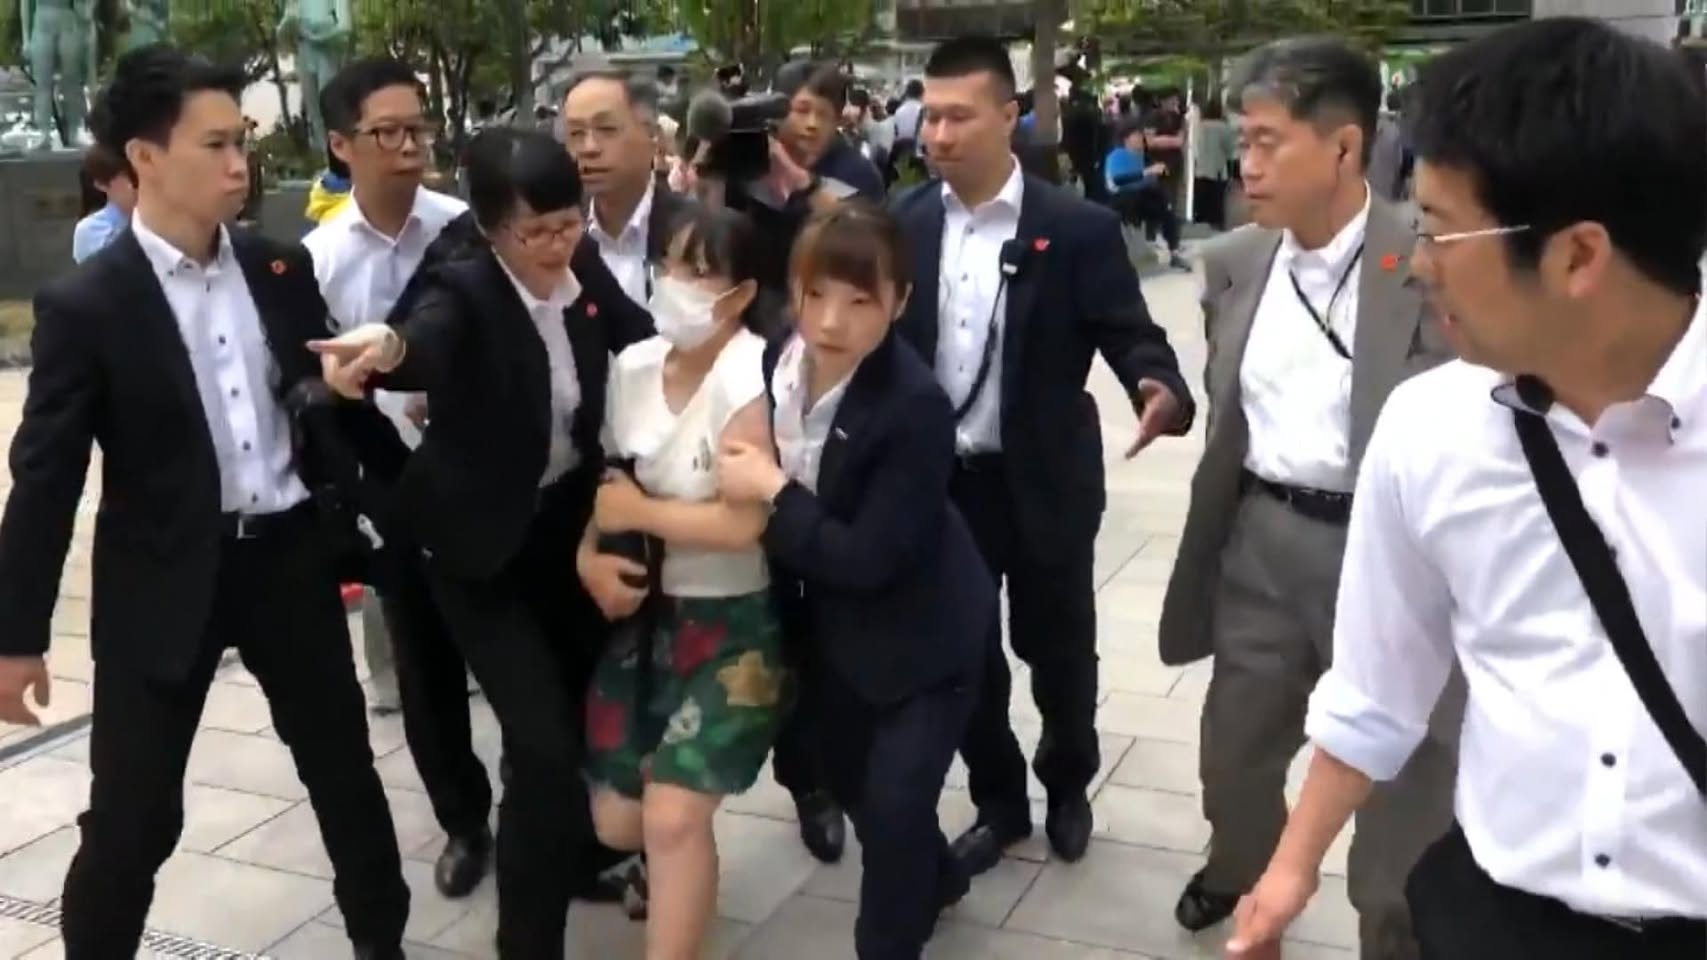
\includegraphics[width=\linewidth]{pictures/2024/01/20240113_002615_001.jpg}
\end{minipage}
\hfill
\begin{minipage}{0.48\linewidth}
\centering
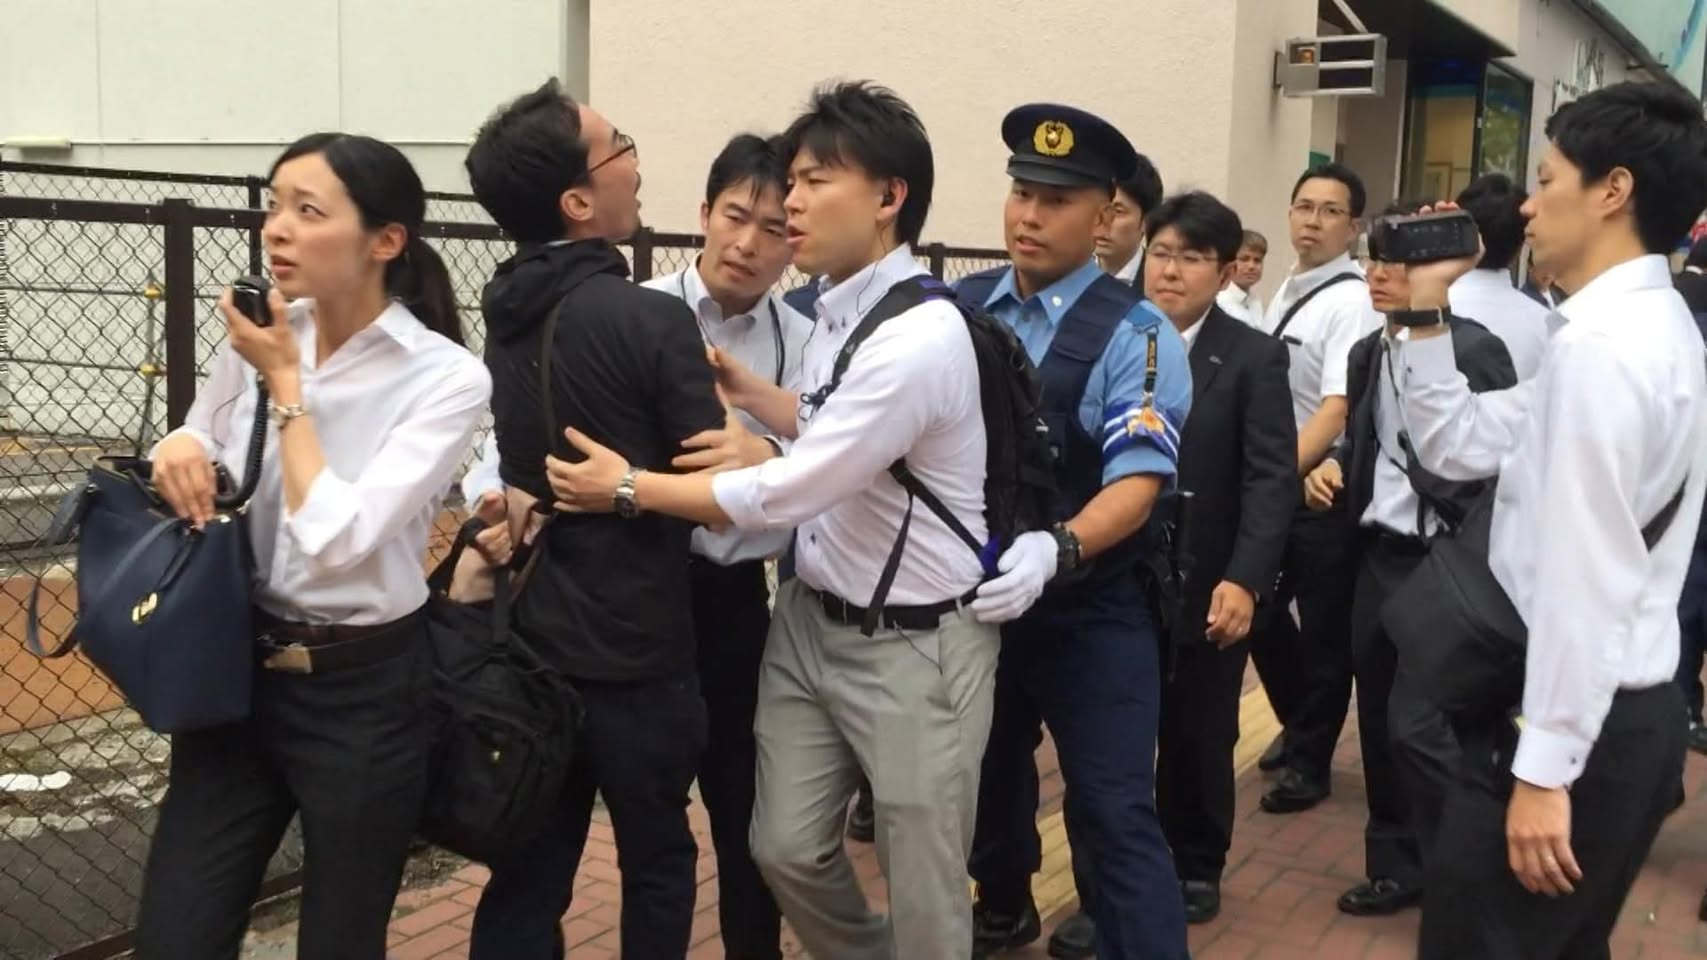
\includegraphics[width=\linewidth]{pictures/2024/01/20240113_002615_002.jpg}
\end{minipage}
\end{center}

\subsection*{2024年01月31日 17:59}
\addcontentsline{toc}{subsection}{2024年01月31日 17:59}

学生時代に \#バーンスタイン の \#マーラー シリーズ(レコードです)を全部手に入れていました。中でも2番アウフ.エルシュテーエンを何度も真剣に（陶酔して？）聞いていたと思います。そして特に第5楽章、ベライテ.ディッヒ！からの目くるめく合唱に興奮していた（時には涙も）記憶があります。当時の事を思い出してみると、若かったんだなと思います。今は（冷静そうな顔をして）「とてもボン.グーとは言えないよな」なんて言ってはみますけど、バーンスタインのこの様な姿を見ると大好きになります。マエストロの棒に合わせて、大きなドラを力一杯叩いて鳴り響かせたくなりますね。

\section{2月}

\subsection*{2024年02月01日 19:22}
\addcontentsline{toc}{subsection}{2024年02月01日 19:22}

今日は最後の班の実習でした。(工業高校2年生)

小信号増幅回路の特性を調べている所です。


「入力と出力の波形見比べて、どう？」

「潰れとるんやけど、、、逆さまになっとるなあ」

「それ、電気科の君なら何て言うの？」

「NOT!」「否定や！」

「うーん、そーう、、だねT君。でも、

もう少しアナログな話したいんだけど、、、」

「え〜ッと、位相が、、、」

「そうそうS君、そうなんだよね。

入力と出力で位相はどうなってる？」

「2分のπ、、、」

「えーー〜っ？、2分のパイいい〜？そうかなア？

よく見てよく見て。もっと単純な格好してるでしょ？」

「180度ズレとる」

「ソーオだよね。That‘s riiiiiiight !!!!

入力の谷の所で出力は山になってるでしょう。

（確かにNOTだねT君）

ところでN君、180度って何ラジアンだった？」


楽しい。こんなちょっとしたやり取りなんだけど、楽しい。

でも、もう今日のこの時間が最後だ。

\paragraph{写真}
\begin{center}
\begin{minipage}{0.48\linewidth}
\centering
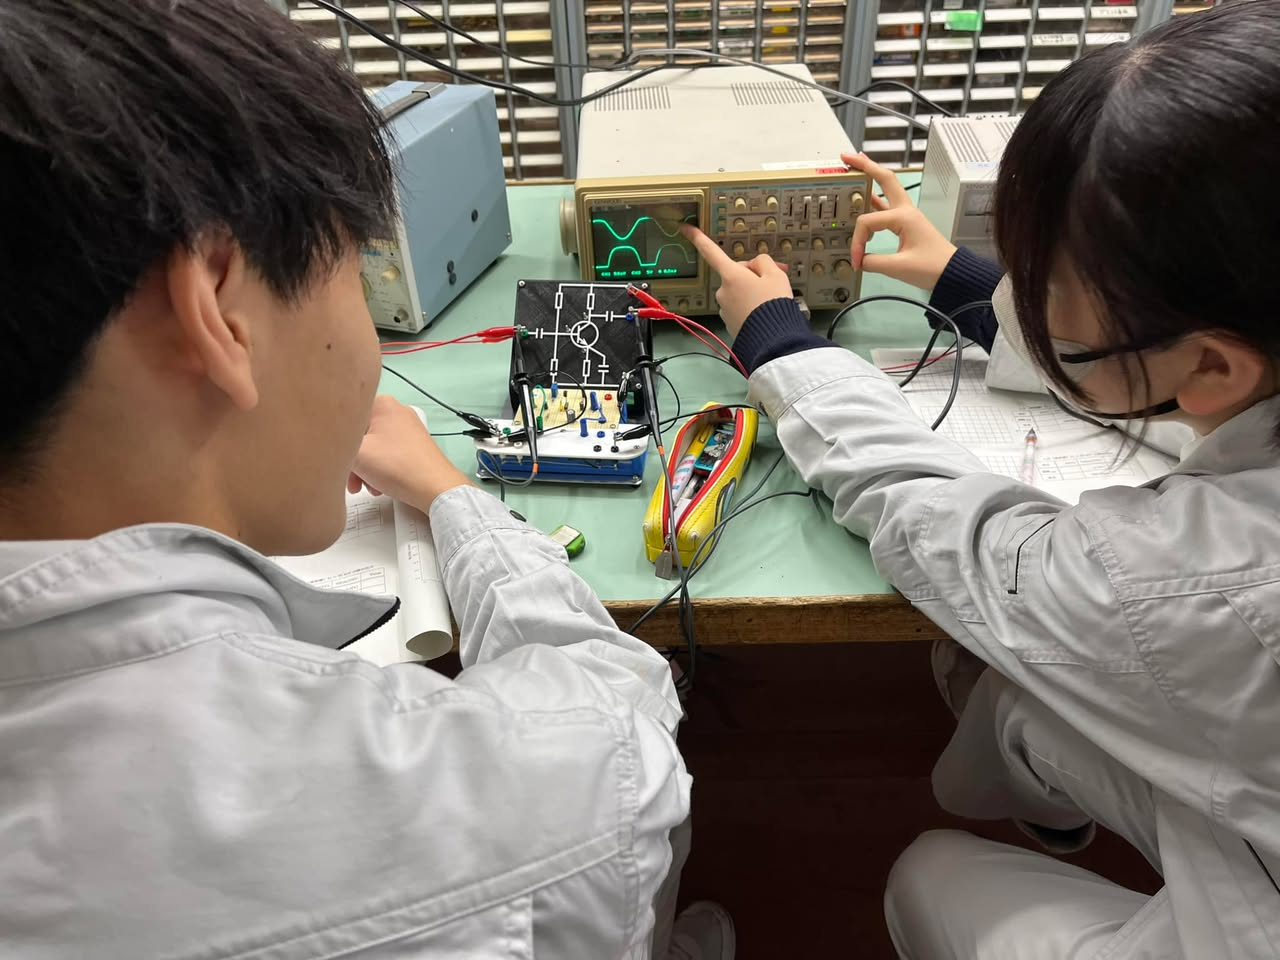
\includegraphics[width=\linewidth]{pictures/2024/02/20240201_192234_001.jpg}
\end{minipage}
\end{center}

\subsection*{2024年02月13日 19:35}
\addcontentsline{toc}{subsection}{2024年02月13日 19:35}

\url{https://www.pythonic-exam.com}




資格を取ろうと思いたった。

今年度いっぱいで高校の講師を辞める予定です。4月以降何もせずに過ごすのもどうかと思い、ネットでアルバイトを探してみた。新入社員教育を請け負っている会社で、試みに（単発ですが）C言語プログラミングのオンライン講師をやってみようという気になった。その会社の講師の方々のプロフィールを見ると、皆さん色々な資格を複数お持ちです。ところが（しがない）私はというと、教員免許（と普通自動車の免許）しか持ち合わせておりません。そこで、一発奮起して資格取得に挑戦してみようと思ったと言うわけです。


とりあえずターゲットに選んだ資格試験は(ここ数年気に入っているプログラム言語から)、「Python 3 エンジニア認定基礎試験」と「Python 3 エンジニア認定データ分析試験」の２つです。前者の試験の公式なテキストブックは「Pythonチュートリアル」で、後者の試験の公式テキストブックは「Pythonによるデータ分析の教科書」だとの事。どちらも70パーセントの正答率で合格になるらしい。手が届きそうな気はしているのですが、どうでしょう（思い上がりでしょうか）。さあて、合格できるかな？

\paragraph{写真}
\begin{center}
\begin{minipage}{0.48\linewidth}
\centering
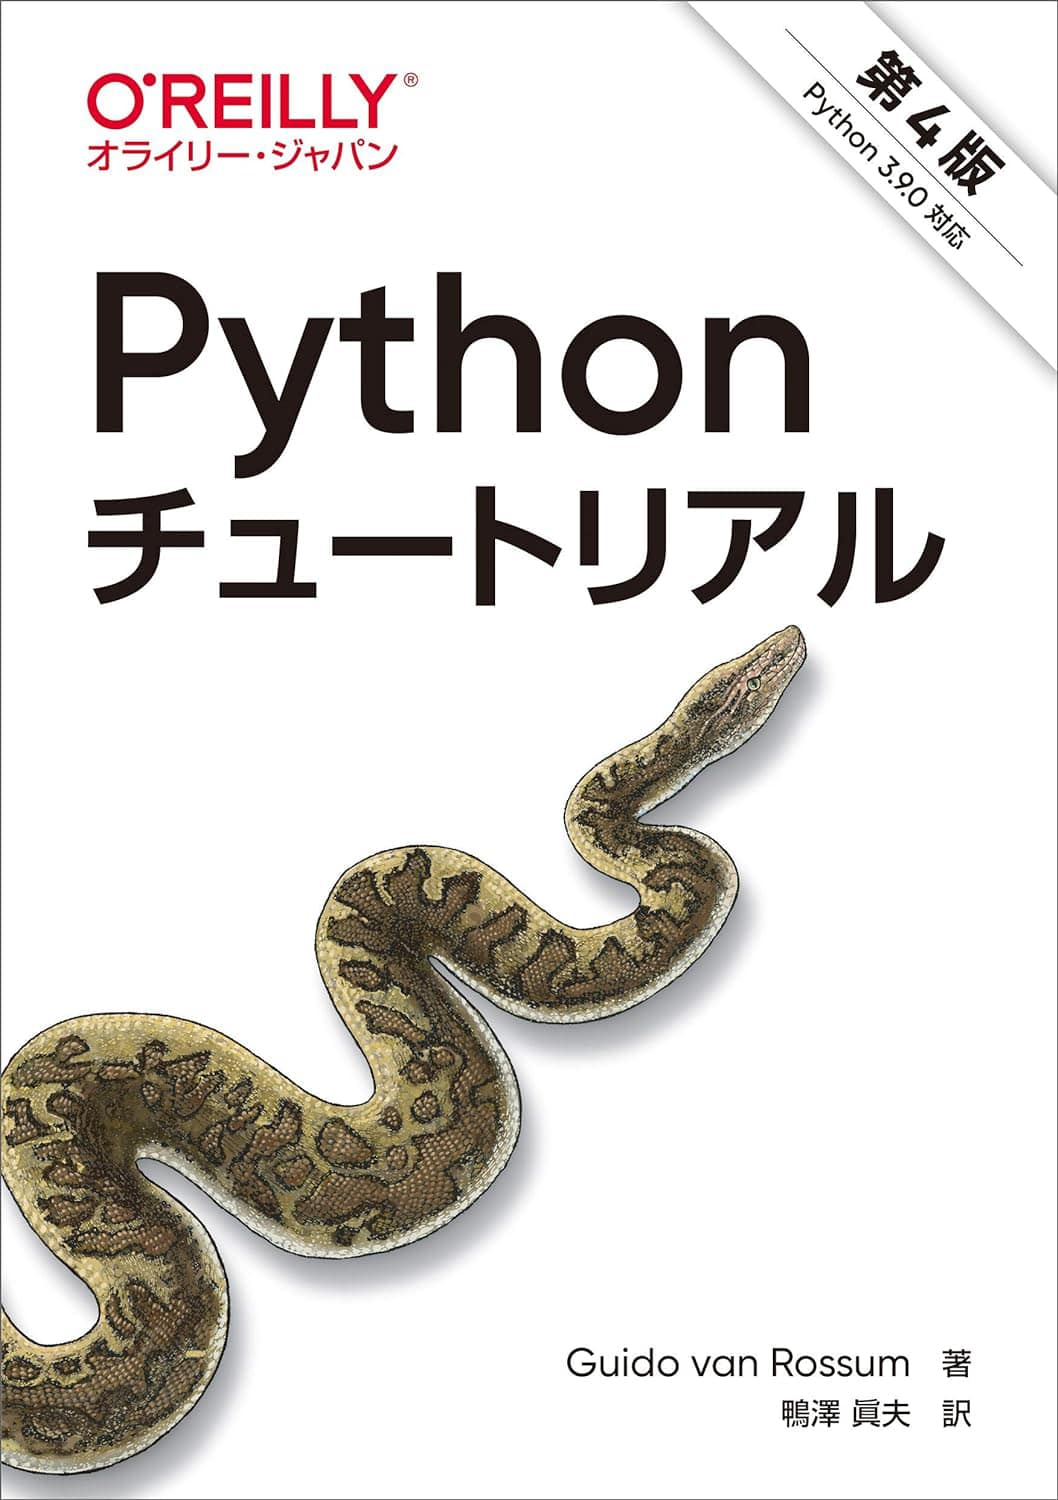
\includegraphics[width=\linewidth]{pictures/2024/02/20240213_193516_001.jpg}
\end{minipage}
\hfill
\begin{minipage}{0.48\linewidth}
\centering
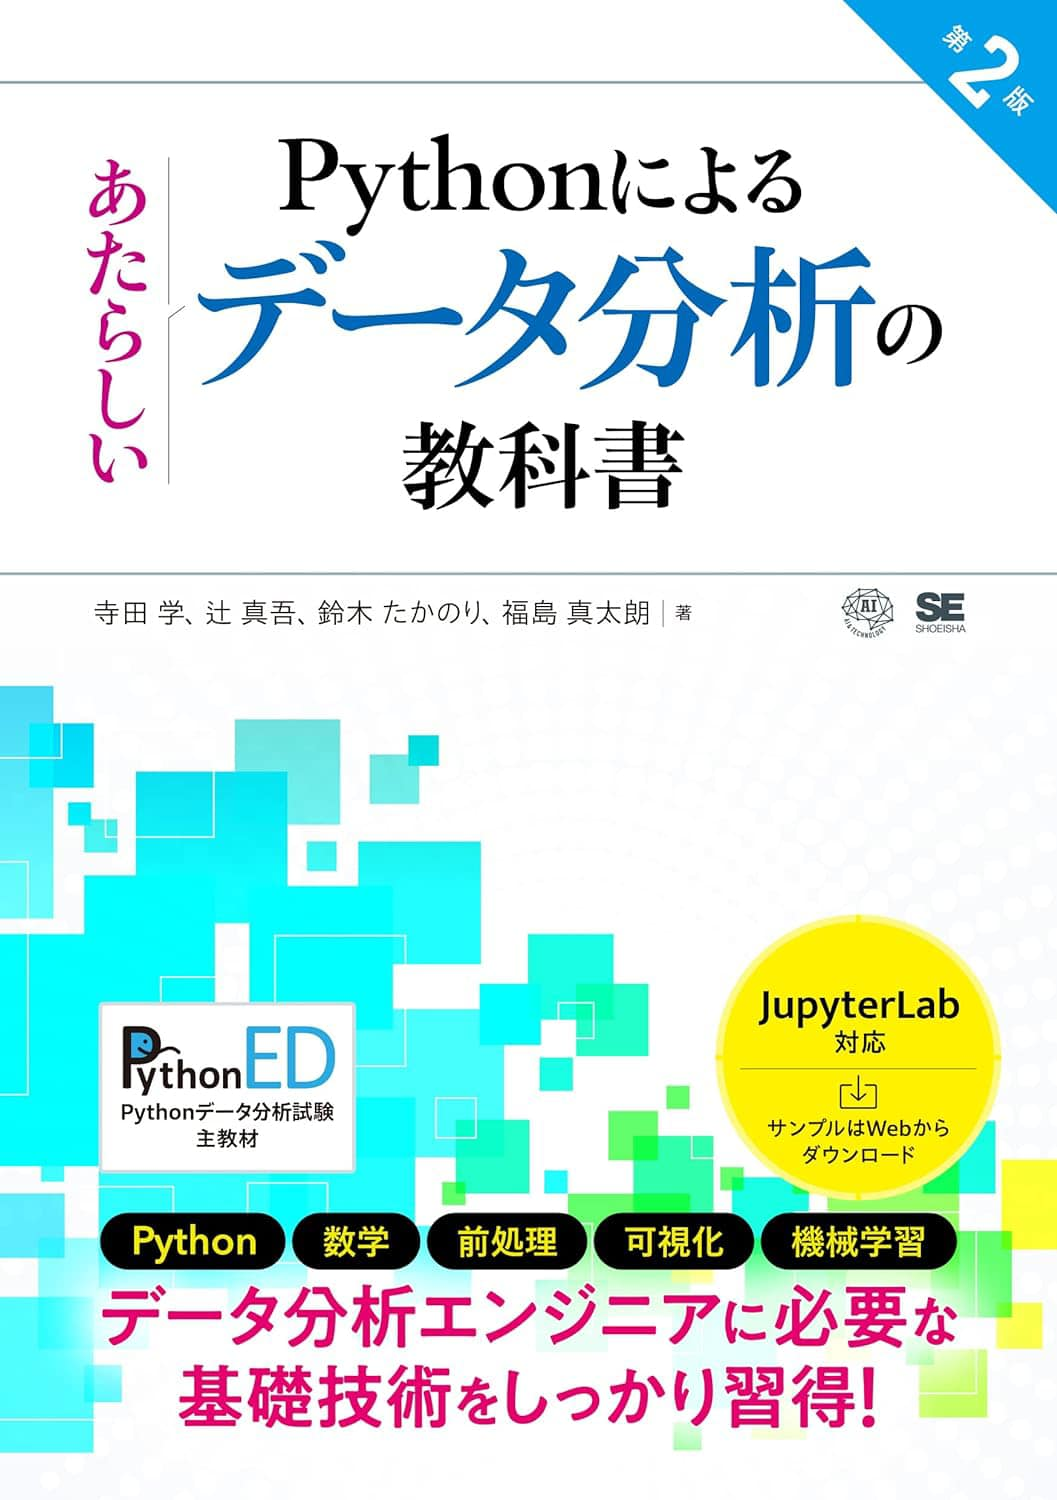
\includegraphics[width=\linewidth]{pictures/2024/02/20240213_193516_002.jpg}
\end{minipage}
\end{center}

\subsection*{2024年02月15日 19:19}
\addcontentsline{toc}{subsection}{2024年02月15日 19:19}

\url{https://x.com/tokoroten/status/1757797075633475735?s=20}




この高校の教科書ですが、完全にPythonが前提になっている。他のプログラム言語の選択肢はない。他の言語では、ゼロからライブラリを作ってかからないと実現できないわけだから、ありえない。


高校教員がこの教科書の内容を指導できる様になるためには、少なくとも「Python 3 エンジニア認定データ分析試験」の範囲（「Pythonによるあたらしいデータ分析の教科書」の後半、第4章のライブラリNumpy、pandas、Matplotlib、scikit-learn以降）はしっかり勉強しておく必要があるんじゃないかな。でも、それはきっと現実にはとても難しい事でしょうね。みんな日々のこまごました業務でとっても忙しいから。教科指導の事を考えて、勉強したり研究したりしている時間はなかなか出てこない（或いは最も後回しになる）でしょう、おそらく。


でもどうでしょうか、例えばscikit-learnで機械学習とか、或いはSQLをプログラムから発行するとか、大方の教員にとって初めて遭遇することのはず。実際にプログラムを書いて動かしながら勉強せざるを得ないと思うんだけど、、、そもそも、そのための環境から作らなきゃいけないし。（何かしらDBMSの動いている環境を用意しないとSQLの発行はできません。）「プログラムしてみたことは無いけど、教科書にはこうなるって書いてあることだし、、、何か、そういう様な事なんじゃないの？とにかく覚えといて、試験に出るよ。」みたいな、ヘナヘナ授業になりはしないか。生徒だけでなく、教員にとってもそんな授業時間は苦痛なだけです。こんな事は杞憂にすぎない事を願っています。

\paragraph{写真}
\begin{center}
\begin{minipage}{0.48\linewidth}
\centering
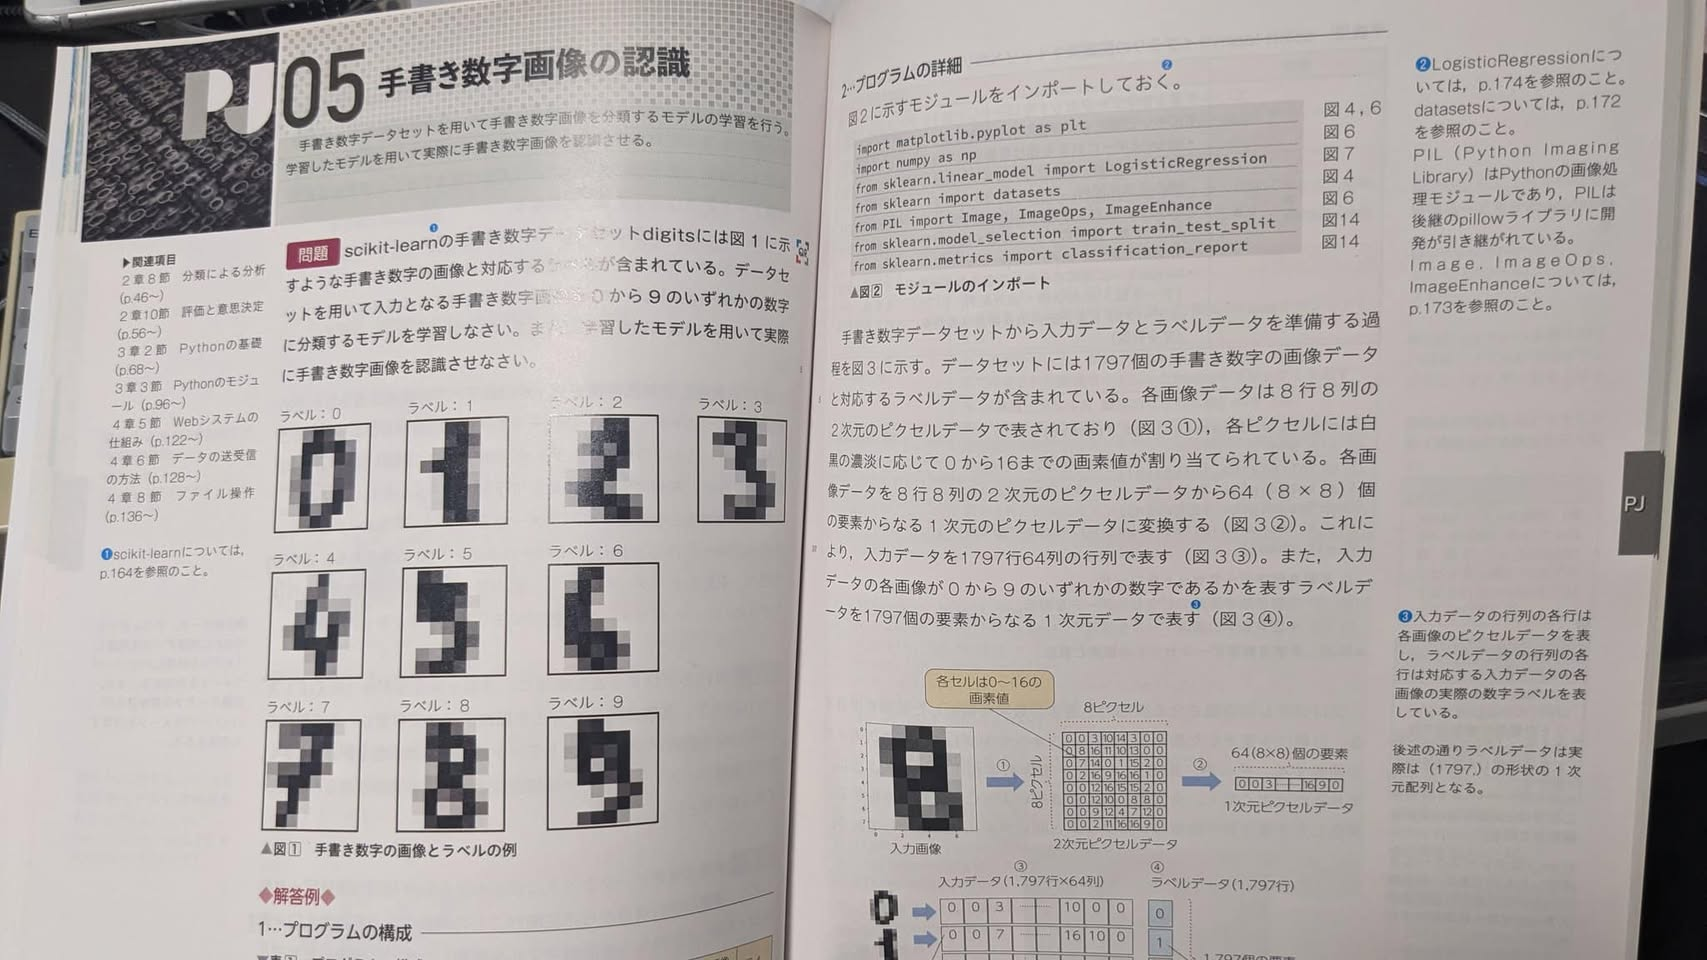
\includegraphics[width=\linewidth]{pictures/2024/02/20240215_191939_001.jpg}
\end{minipage}
\hfill
\begin{minipage}{0.48\linewidth}
\centering
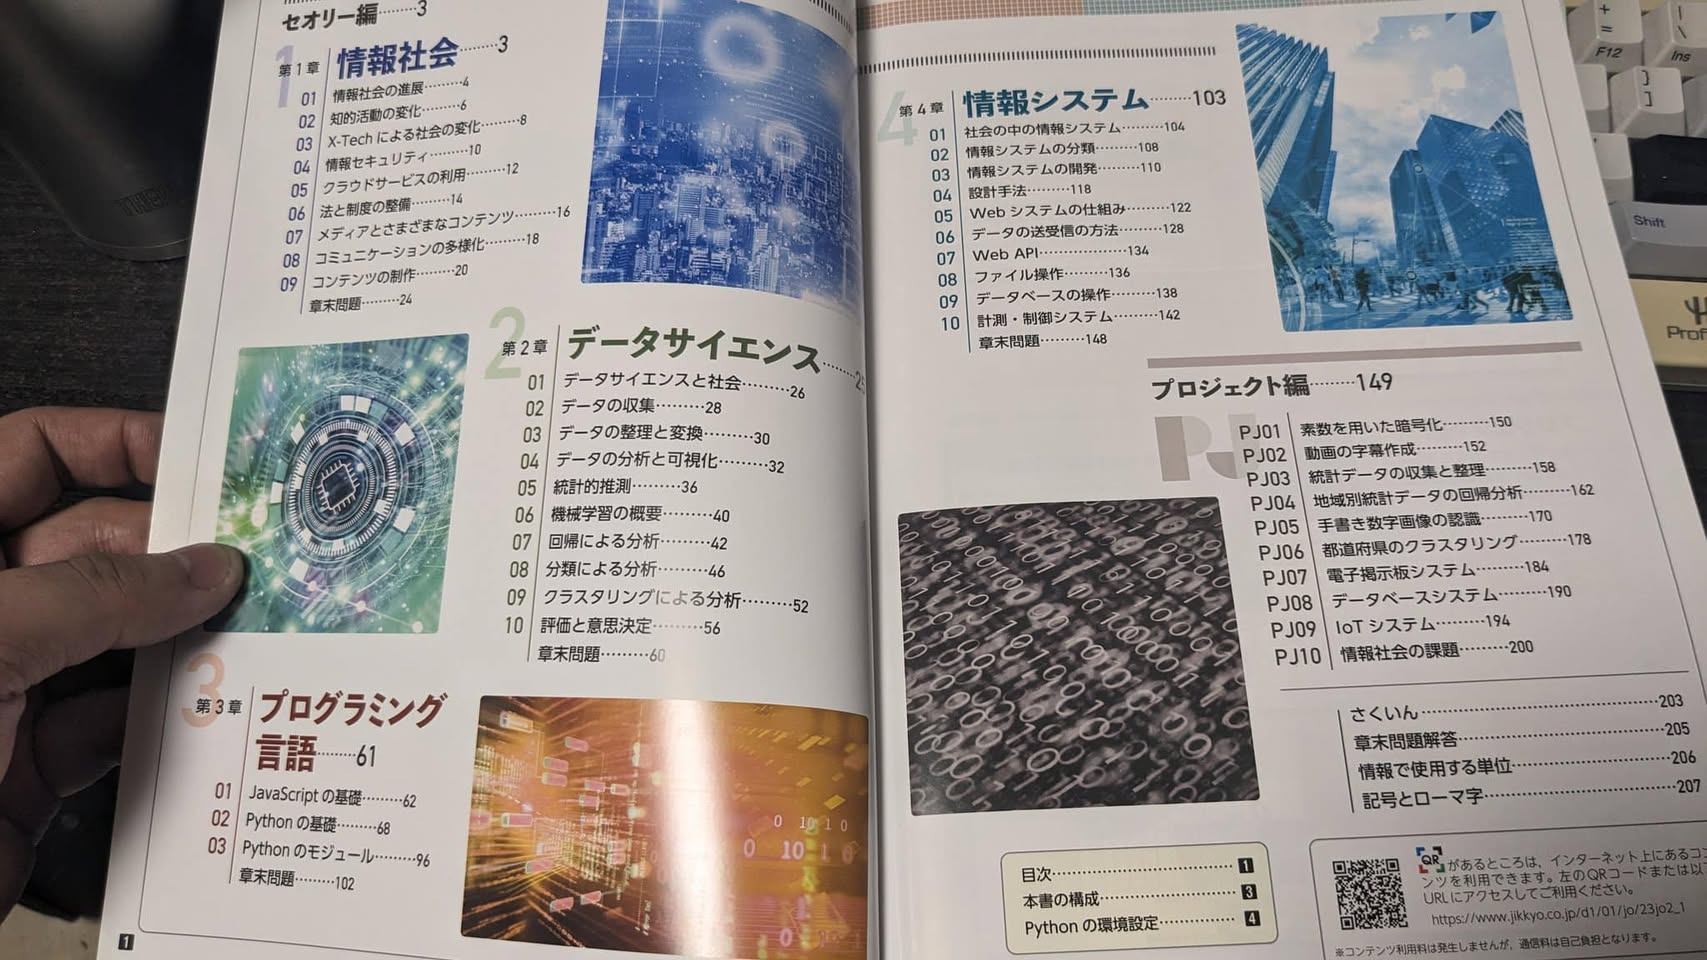
\includegraphics[width=\linewidth]{pictures/2024/02/20240215_191939_002.jpg}
\end{minipage}
\end{center}

\subsection*{2024年02月16日 04:11}
\addcontentsline{toc}{subsection}{2024年02月16日 04:11}

資格取得について、Pythonに続く次のターゲットを検討し始めた。しかし、これは、、、受験料が高いのでやめとこうと思い始めている。個人を対象としていないようだ。事業者が、スキルを持っている会社なんだと対外的に示すため、客観的指標として使われるものなのでしょうか。それにしても、本当にtoo expensive だ！


Linuxには、国際資格のLPICと、より実践的とされる日本版の資格LinuCの２つがあって、どちらの資格も試験レベル毎に２つの試験に合格する必要がある。レベル1の２つの試験（101試験、102試験）の合格が、レベル2の２つの試験（201試験、202試験）の受験資格になっている。つまり、レベル1から順に受けなさいということ。合否のラインは推定で65\%程。ただし、合格した資格の有意性は５年間とされている。


Oracle認定Javaプログラマの資格は、時代に対応して新しくなってきている様だ。最新（2023年12月以降）の資格はSE17（その前はSE11だった）らしい。Goldレベルの受験にはSilver資格を持っている事が前提だが、Silver資格とBronze資格に前提条件は無い。従って、SE17のSilver資格をとるのがよい。（Bronze資格はskipできる）合格ラインは65\%


どの資格も受験料がとても高いので、何度も挑戦して取得を目指すという類のものではない。受けるのならきちんと対策して一発合格にすべきものだろう。難易度が気になって問題集を探してみたが、JavaのSE17対応のものは2月21日発売予定みたいだ。（問題を解き始めたら受けてみたくなるかもしれない）

\paragraph{写真}
\begin{center}
\begin{minipage}{0.48\linewidth}
\centering

\includegraphics[width=\linewidth]{pictures/2024/02/20240216_041112_001.jpg}
\end{minipage}
\hfill
\begin{minipage}{0.48\linewidth}
\centering

\includegraphics[width=\linewidth]{pictures/2024/02/20240216_041112_002.jpg}
\end{minipage}
\end{center}

\subsection*{2024年02月17日 02:57}
\addcontentsline{toc}{subsection}{2024年02月17日 02:57}

Pythonの４つ目の資格試験が新しく始まるようだ。どんな内容なのか少し気になっている。


主教材とされている「Pythonデータ分析 実践ハンドブック 実務で使えるデータ加工のテクニック」（インプレス）の試し読みにアクセスしてみた。データサイエンティストとデータ分析エンジニアとの役割分担の様な事が書かれている。実はデータサイエンスについて数年前から注目していた。大学でも新しい学部やコースの様な形で新設されてきている様だ。データサイエンティストにとってPythonのスキルはある程度は必要だろう。しかし、プロフェッショナルなプログラマである必要はない。それはデータ分析エンジニアが担います、という事なのだろう。データ分析エンジニアというものを別に用意する事によって、数学的（或いは科学的、経済的、社会的などの）専門知識の持ち主である専門家としてのデータサイエンティストと、実務家としてのデータ分析エンジニアとの住み分けを計り、協力体制を作ろうという流れなのだなと理解した。

\paragraph{リンク}
\url{https://cloud.watch.impress.co.jp/docs/news/1569059.html}

\subsection*{2024年02月18日 06:32}
\addcontentsline{toc}{subsection}{2024年02月18日 06:32}

\url{https://m.facebook.com/story.php?story_fbid=7130496700367763&id=100002225117991}




最近「課題解決のための統計的な思考」に興味があります。

本を読みながら、時々入試データ処理の事を思い出しています。横軸と縦軸それぞれ何点満点だったっけ？少なくとも「正規化したデータ」の散布図上で線を引くとよかったのでは？正規化するならz変換するより最小最大正規化の方がピンと来るんじゃないかな？でも、正規化しても散布図の絵面って変わらないんじゃない？はじめに特徴量ごとのデータを持たせた表を作る必要があるね。いやいや、最初のデータ入力作業はこれまで通り Excelで行い、それをpandasで読み込んでDataFrameにすればPythonの世界に持ち込めるね。クラスタリングしてみるとどうなる？などなど。いろいろな事に思いを巡らせてはいるけど、これらを試してみる機会はもうありませんね。（失敗したら大変な事だから、それはそれでよかったよ。触らぬ神に祟りなし。クワバラ、くわばら。）

\paragraph{写真}
\begin{center}
\begin{minipage}{0.48\linewidth}
\centering
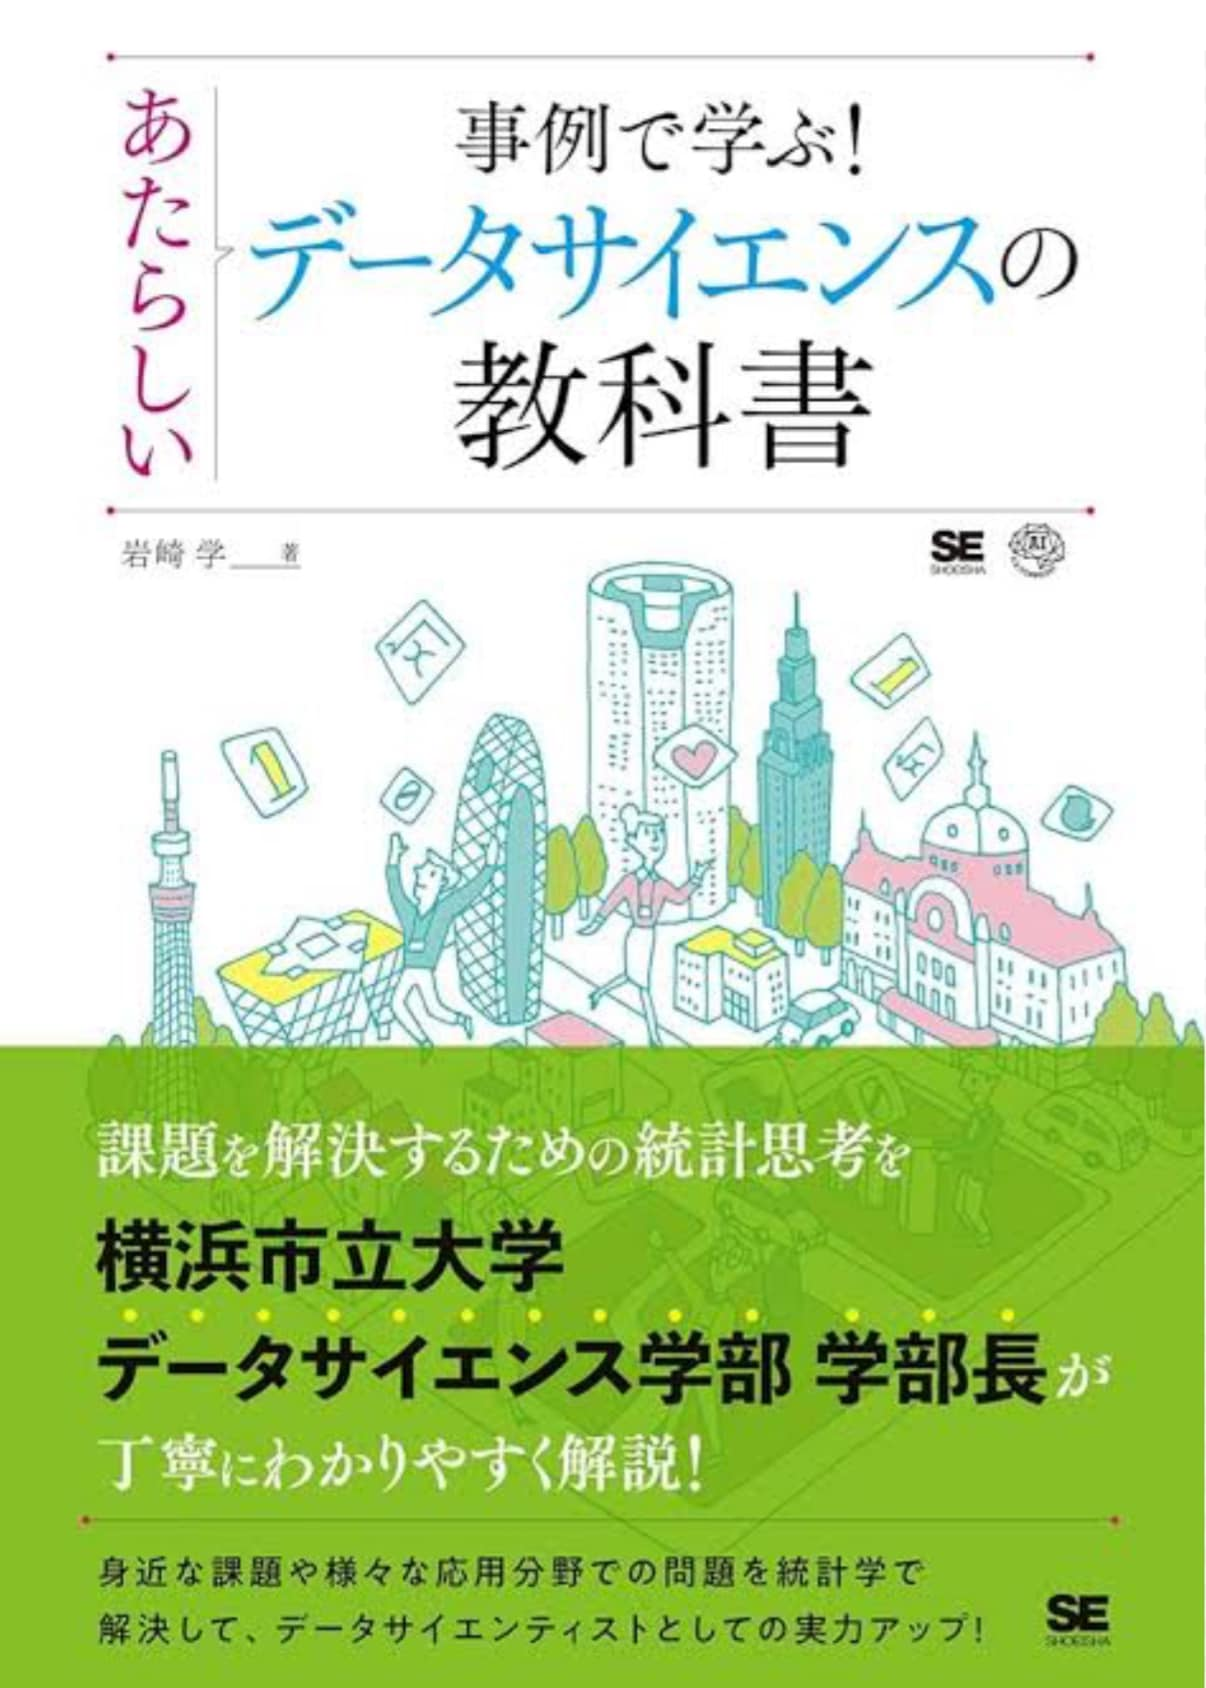
\includegraphics[width=\linewidth]{pictures/2024/02/20240218_063249_001.jpg}
\end{minipage}
\hfill
\begin{minipage}{0.48\linewidth}
\centering
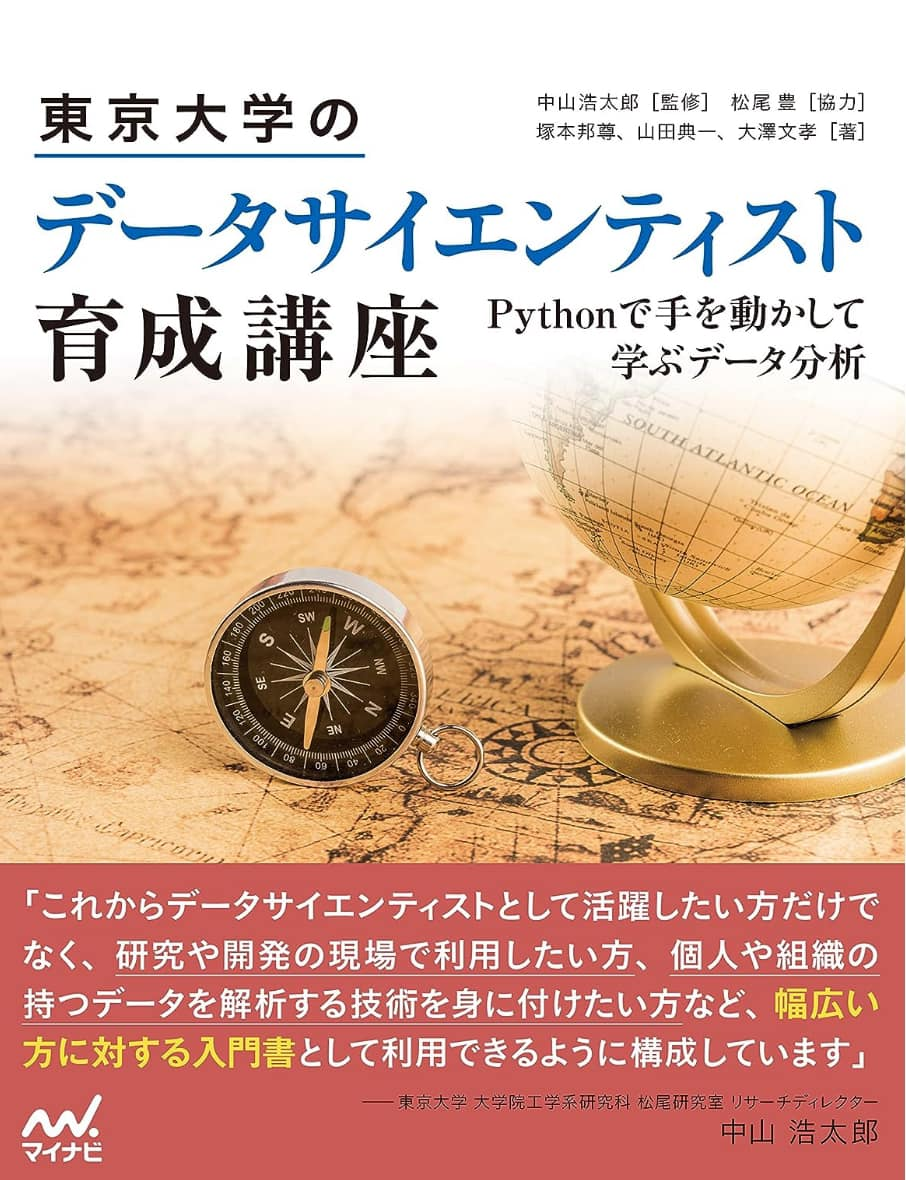
\includegraphics[width=\linewidth]{pictures/2024/02/20240218_063249_002.jpg}
\end{minipage}
\end{center}

\subsection*{2024年02月18日 14:34}
\addcontentsline{toc}{subsection}{2024年02月18日 14:34}

\url{https://video.twimg.com/ext_tw_video/1655447139353497600/pu/vid/320x568/PBp74pzfLezxCK1v.mp4?tag=12}




ほんとだー！

国防費やオリンピック、大阪万博は、予算無視、無条件で承認だが、それらよりずっと少ない予算規模の少子化対策、生活保護などの話題になった途端、予算の当てはどうするのという話になる。と言うことは即ち、予め為政者が決めた優先順位があって、それに従って判断されるので「少子化対策や生活保護は二の次」と言う事になる。更には「いつまで経っても」二の次に置かれているので、いつになっても決して対策される時は来ない。そんな事でいいのかな？

\paragraph{写真}
\begin{center}
\begin{minipage}{0.48\linewidth}
\centering
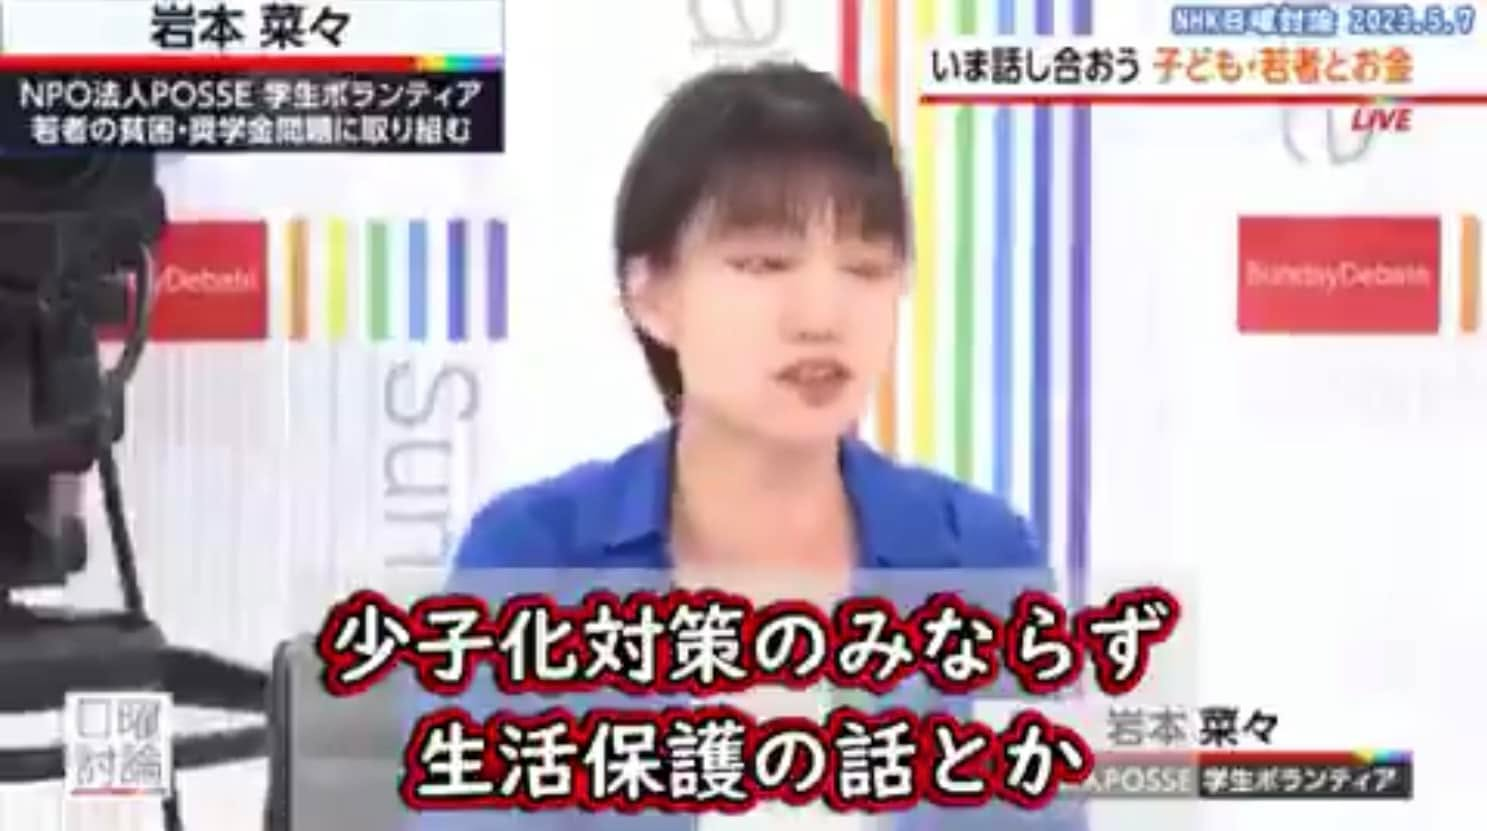
\includegraphics[width=\linewidth]{pictures/2024/02/20240218_143438_001.jpg}
\end{minipage}
\end{center}

\subsection*{2024年02月26日 08:17}
\addcontentsline{toc}{subsection}{2024年02月26日 08:17}

JupyterLabの環境下でPythonのデータ分析試験の対策をしていたら、JupyterLabが気に入ってきた。（Jupyterはプログラム言語のJulia、Python、Rが語源になっているとのこと）Rでも使えるようにしようと思った。（以下は、Macのターミナル上での話です）


（1）Pythonのvenv環境に入って

（2）Rを起動してRのプロンプト＞が出たら

（3）> install.packages('IRkernel')

（4）> IRkernel::installspec()

（5）> quit()  でRを抜けて


後はJupyterLabを起動したら添付の画面の通り、RのNotebookを選べるようになっていました。めでたしめでたし。（ただしこの環境が、Pythonのvenv環境に依存するものなのかどうか？新しいvenv 環境を作ってみれば分かることだけど、それはそのうち試してみる事にしよう。）

\paragraph{写真}
\begin{center}
\begin{minipage}{0.48\linewidth}
\centering
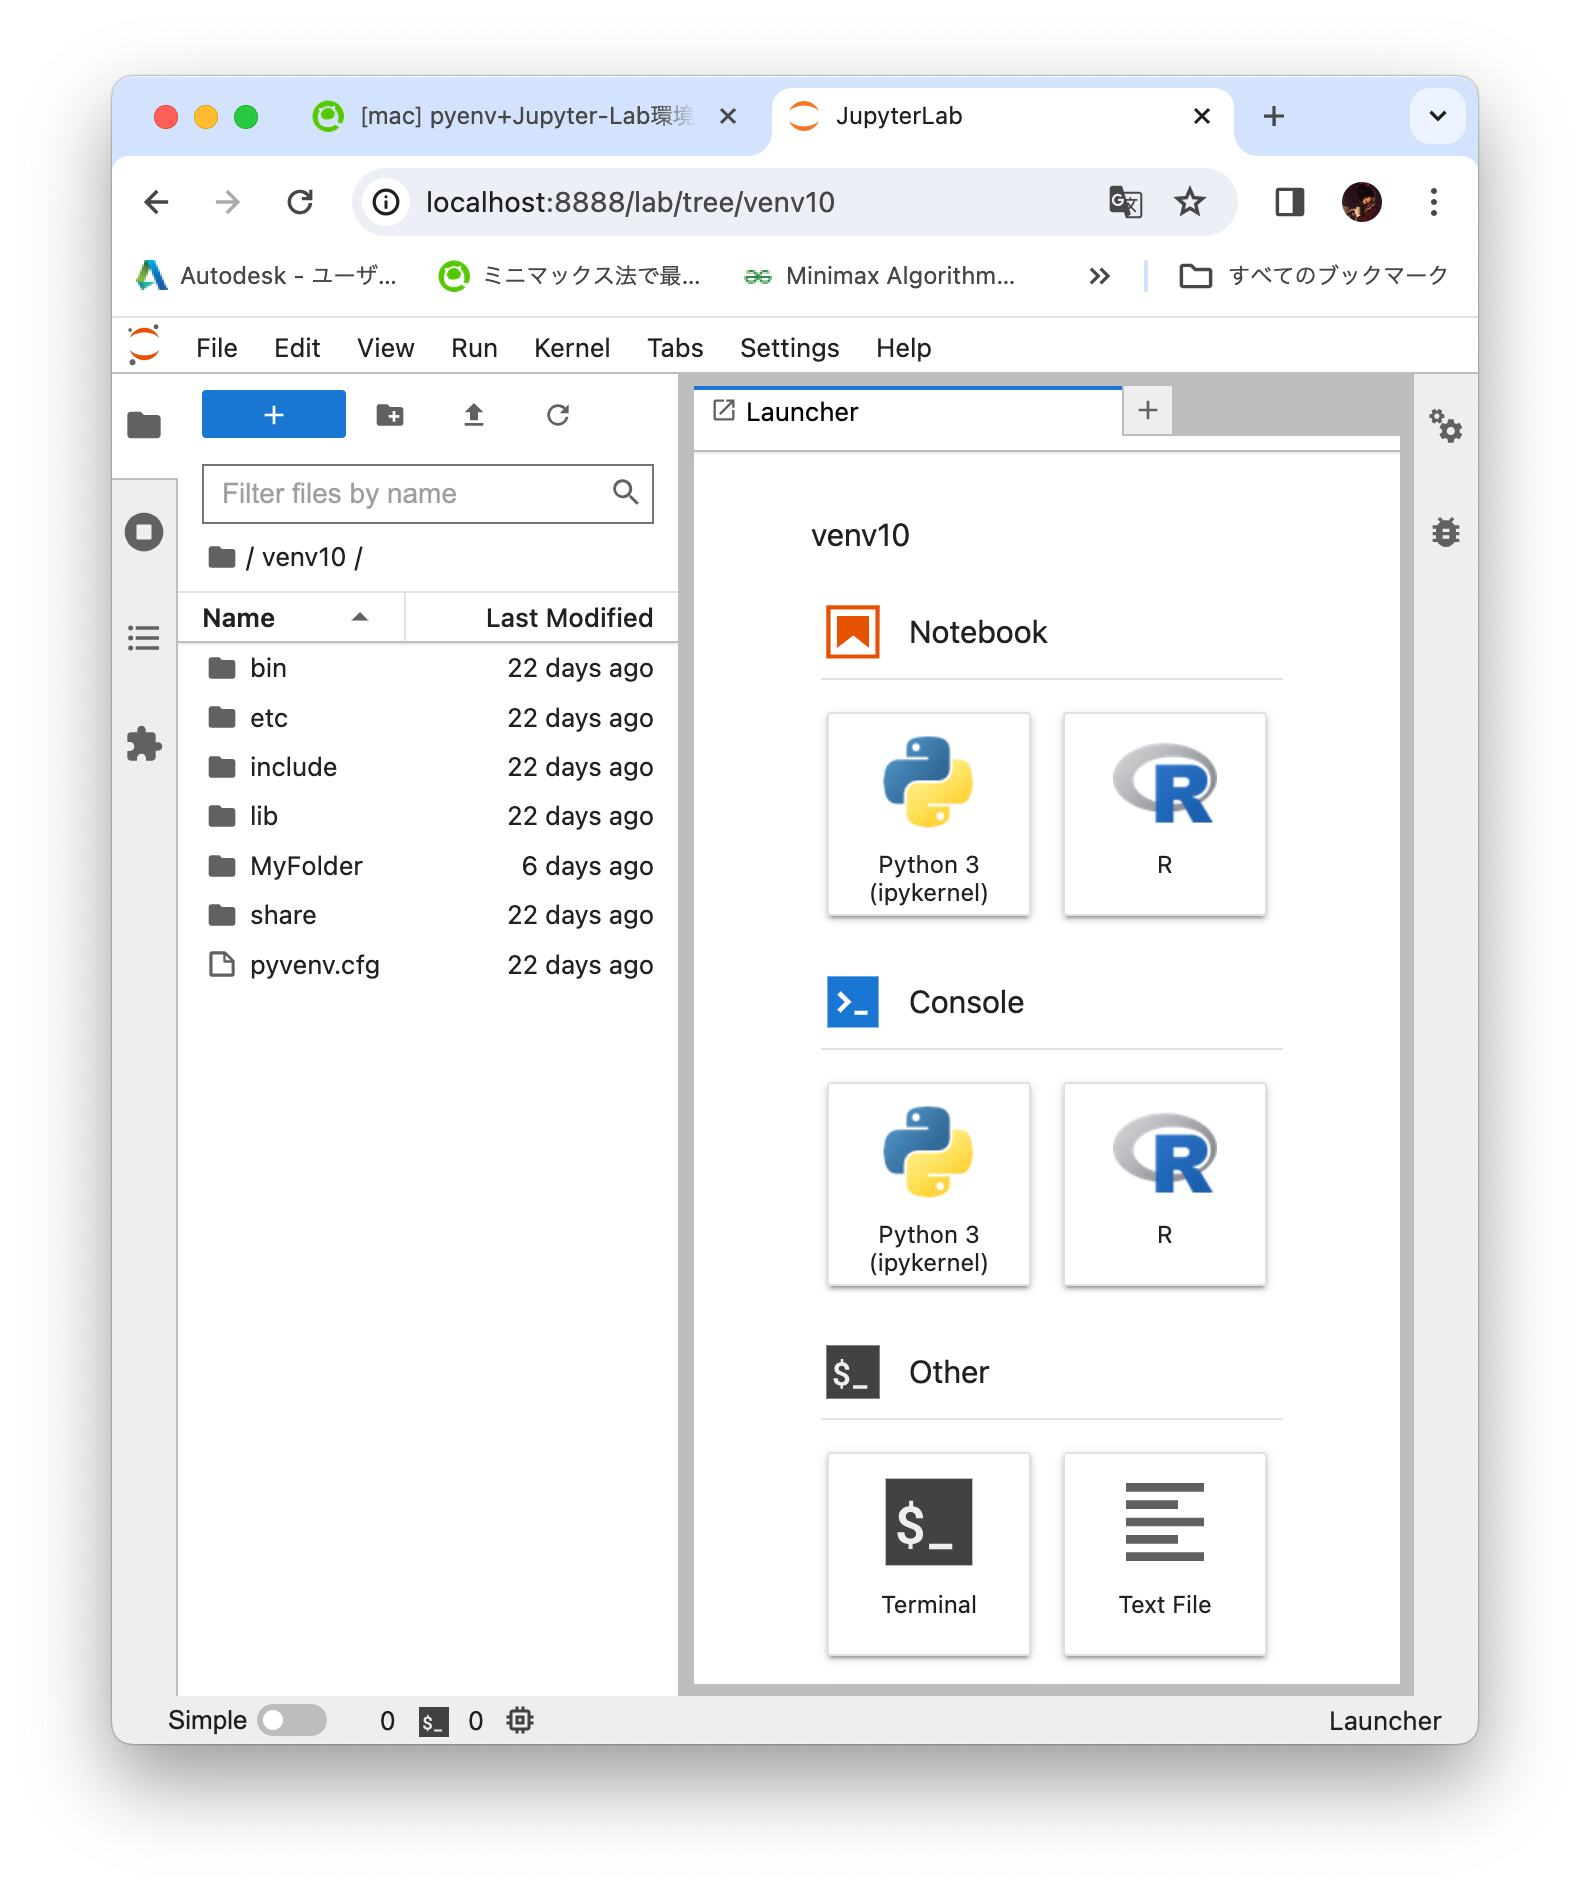
\includegraphics[width=\linewidth]{pictures/2024/02/20240226_081730_001.jpg}
\end{minipage}
\end{center}

\section{3月}

\subsection*{2024年03月10日 14:35}
\addcontentsline{toc}{subsection}{2024年03月10日 14:35}

\url{https://bookclub.kodansha.co.jp/product?item=0000349808}




ドキュメント編を読みました。（検証編は未だ手に入っていない）

運転中だった1号機と3号機、そして運転を停止していた4号機までも、順に水素爆発を起こした。2号機は原子炉格納容器の爆発までもが心配される中、（何故か）爆発を逃れている。格納容器と配管との接合部の溶融や容器上部のフランジとの繋ぎ目から、大量の放射線を含む蒸気が漏れ出していたため格納容器の爆発には至らなかったのだという。（漏れた事が幸いして爆発に至らなかったとは言え、そもそも漏れるという事自体問題だったはず。）なお、チェルノブイリ（チェルノービル）発電所の事故では原子炉が爆発している。もし2号機の原子炉格納容器が爆発していたら、チェルノービル同様、東京都を含む神奈川県にまで至る東日本一帯が居住不可になる事態が予想された。

どのプラントの場合も、原子炉冷却のため格納容器に注水しようとしていたが、そのためには、格納容器内の圧力（70気圧）を下げてからでないと、消防車（9気圧）による注水はできなかった。格納容器内の圧力を下げるためにベント（ウェットウェルやドライウェル）や、SR弁の開放などといった手立てを取ろうとしていたんだという事がわかる。更には、消防車からの注水も、格納容器に至るまでのプラントの経路が複雑に分岐しているため、原子炉内への注水に至る前段で分岐して漏水し、殆ど原子炉格納容器の冷却にまで至っていなかったらしい。

翻って能登の地震の際、運転を停止していたとはいえ、使用済み核燃料を水槽内に浸して貯蔵しているであろう北陸電力の志賀原子力発電所だが、地震後も原子炉の施設設備は健全であるという報告が上げられていたのだろうか、現政府には全く危機感がなかった（総理は政財界の皆さんとの新年会に出席していらした）事を思い出した。私たちは、13年前の福島の事を忘れてしまっていたのですね、きっと。

\paragraph{写真}
\begin{center}
\begin{minipage}{0.48\linewidth}
\centering
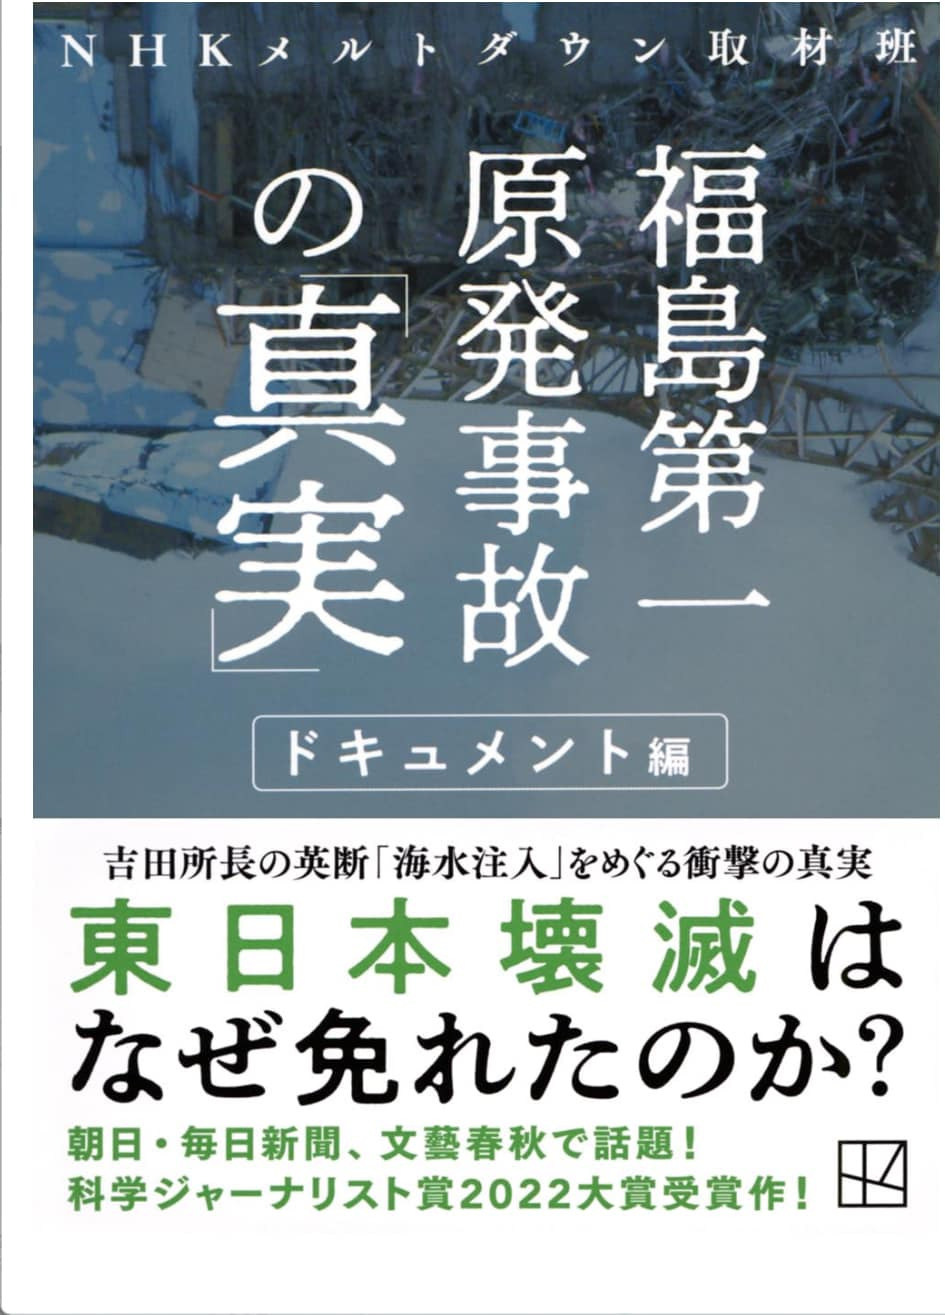
\includegraphics[width=\linewidth]{pictures/2024/03/20240310_143508_001.jpg}
\end{minipage}
\hfill
\begin{minipage}{0.48\linewidth}
\centering
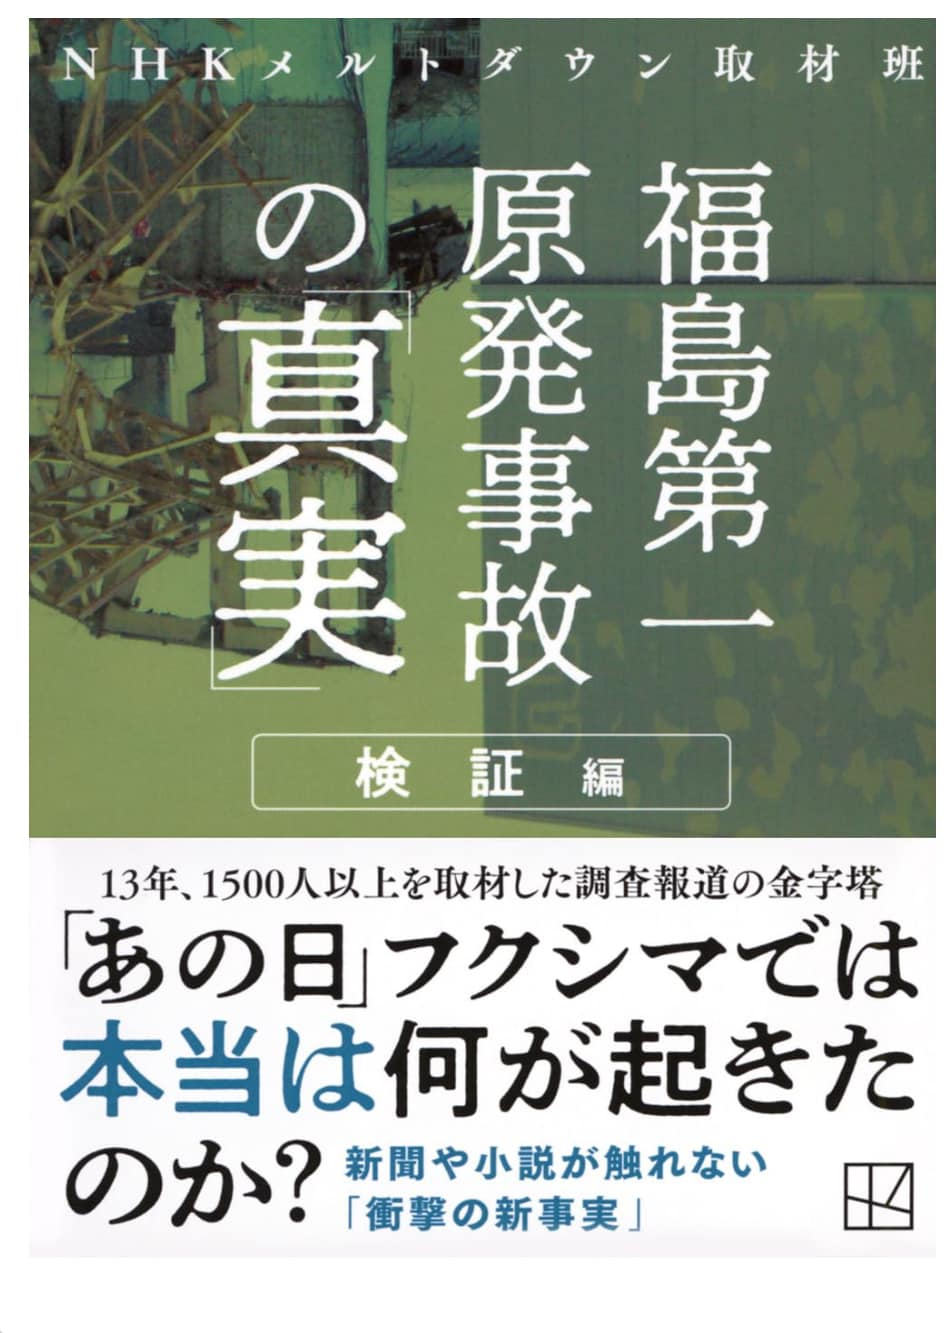
\includegraphics[width=\linewidth]{pictures/2024/03/20240310_143508_002.jpg}
\end{minipage}
\end{center}

\subsection*{2024年03月29日 18:04}
\addcontentsline{toc}{subsection}{2024年03月29日 18:04}

とても興味があります。

高校の時に世界史を選択して暗記モノに辟易としてしまい、歴史大嫌いになっていた私ですが、この歳になった今となっては、お話としてチンタラ読むのならOkです。

日本史なんかは、先ず外国の方の読者を期待しますし、日本人でも通訳を生業としていらして、日本を外国の方に紹介する機会などに（正確な情報が得られて）重宝するんじゃないかな。

無理やりの、Front-Squared-Back-Circled？-Shaped kofunをp.23で確認したくなってきました。The kofun has the shape of squared front with circled back. 「後ろに円形がくっついている四角い前の形の古墳」はどう？めちゃくちゃか？まさか、とは思うけど、zenpokoen-shaped kofunの類か？そんな事を考えていると、この本の表紙の絵柄、黒い影ですが、方形と円形が一部重なっていますね。（そのうちAmazonでポチっているかもしれない）


\#山川出版社 \#日本史 \#世界史 \#教科書

\paragraph{写真}
\begin{center}
\begin{minipage}{0.48\linewidth}
\centering

\includegraphics[width=\linewidth]{pictures/2024/03/20240329_180409_001.jpg}
\end{minipage}
\hfill
\begin{minipage}{0.48\linewidth}
\centering

\includegraphics[width=\linewidth]{pictures/2024/03/20240329_180409_002.jpg}
\end{minipage}
\end{center}

\subsection*{2024年03月31日 19:51}
\addcontentsline{toc}{subsection}{2024年03月31日 19:51}

英語版の詳説日本史を手に入れて（初めから順番に）読み？はじめた。でも、そもそも、初めから順番に（時代の流れに沿って）読み進めなきゃいけないのかな？これは。


読むのにとても疲れる？ので、、、、同社の日本語の教科書を入手する事にした。（やっぱりそうなったか、結局。）また同時に、図録と言うのも面白そうだったので購入してしまった。


最初から順番に読む必要などないのだ。興味のある所、時代や人物をつまみ食いすればよい。NHKの大河ドラマを見ていて、「え〜っと、あれは藤原の、、、誰だっけ」となれば、そのページ周辺を参照すればよいだけのこと。何よりも試験対策ではないのだから「覚えなくてよい」。このことは実に素晴らしいことだ。特に図録はカラーも綺麗だし、図や写真を眺めながら、気軽に短いキャプションを読んでいる感じで面白い。図録だけでも時代の流れなど、ある程度分かるものなのですね。分かりやすく出来てるなあ。一方で教科書の方を見ていると、漢字のルビが随所に入れられている（ルビがないととても読めそうにない固有名詞の類がたくさんある）ので、年寄りの目は点になりそうです。


それにしても受験生は大変だ。こんなに細かいたくさんのことを覚えなくちゃいけないものなのか。同情するしかないな。


\#山川出版 \#日本史 \#教科書

\paragraph{写真}
\begin{center}
\begin{minipage}{0.48\linewidth}
\centering
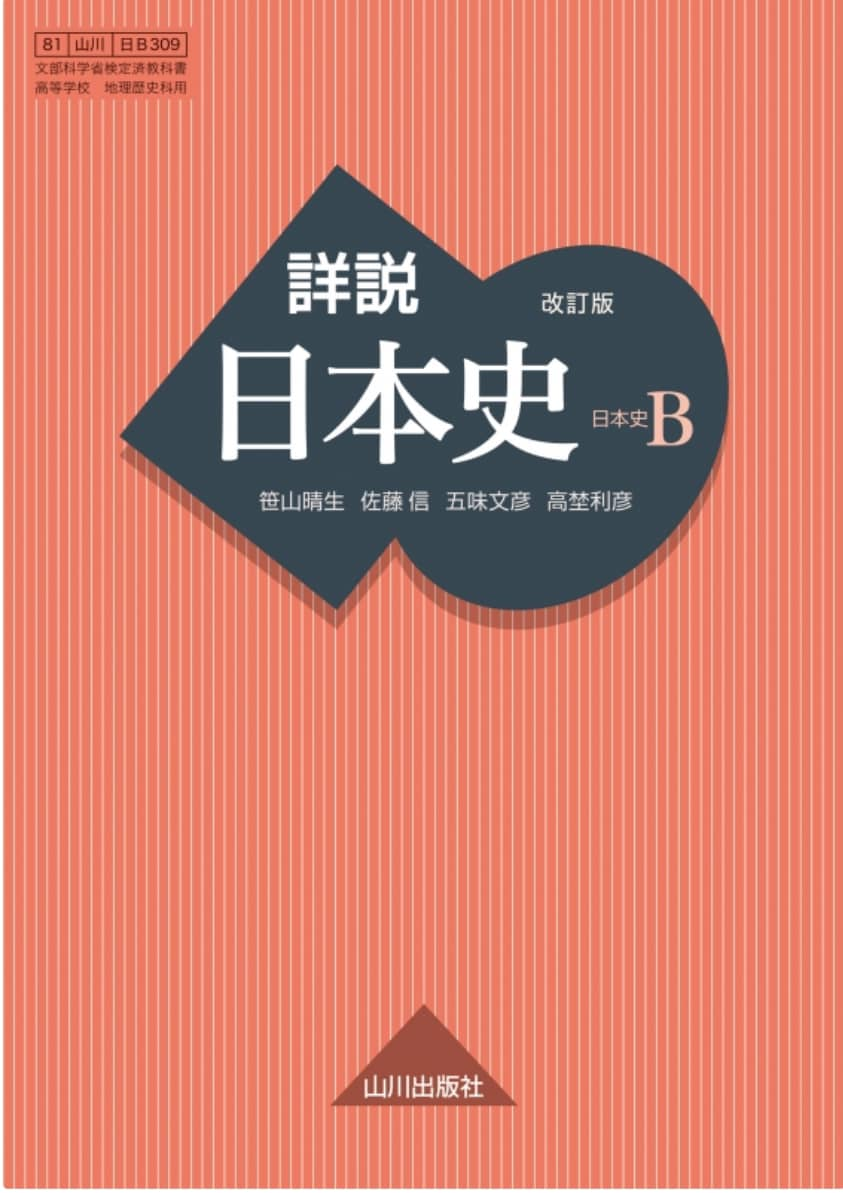
\includegraphics[width=\linewidth]{pictures/2024/03/20240331_195114_001.jpg}
\end{minipage}
\hfill
\begin{minipage}{0.48\linewidth}
\centering
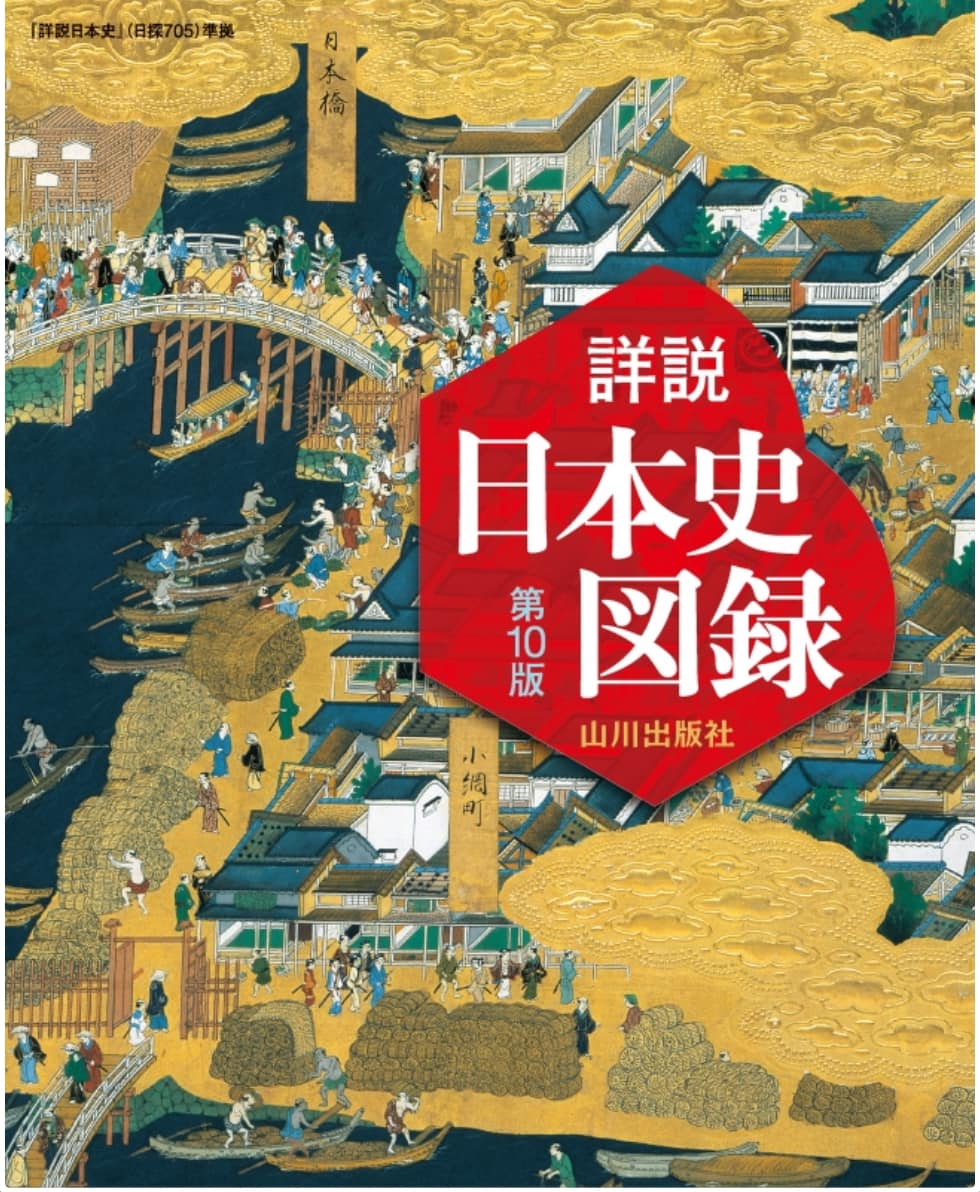
\includegraphics[width=\linewidth]{pictures/2024/03/20240331_195114_002.jpg}
\end{minipage}
\end{center}

\section{4月}

\subsection*{2024年04月10日 13:36}
\addcontentsline{toc}{subsection}{2024年04月10日 13:36}

\#金沢 は至る所、\#桜 でいっぱいです。（人もいっぱいですが）

（裏門がこんなに人気になるとは、お殿様も想像しなかったことでしょうね。）

\paragraph{写真}
\begin{center}
\begin{minipage}{0.48\linewidth}
\centering
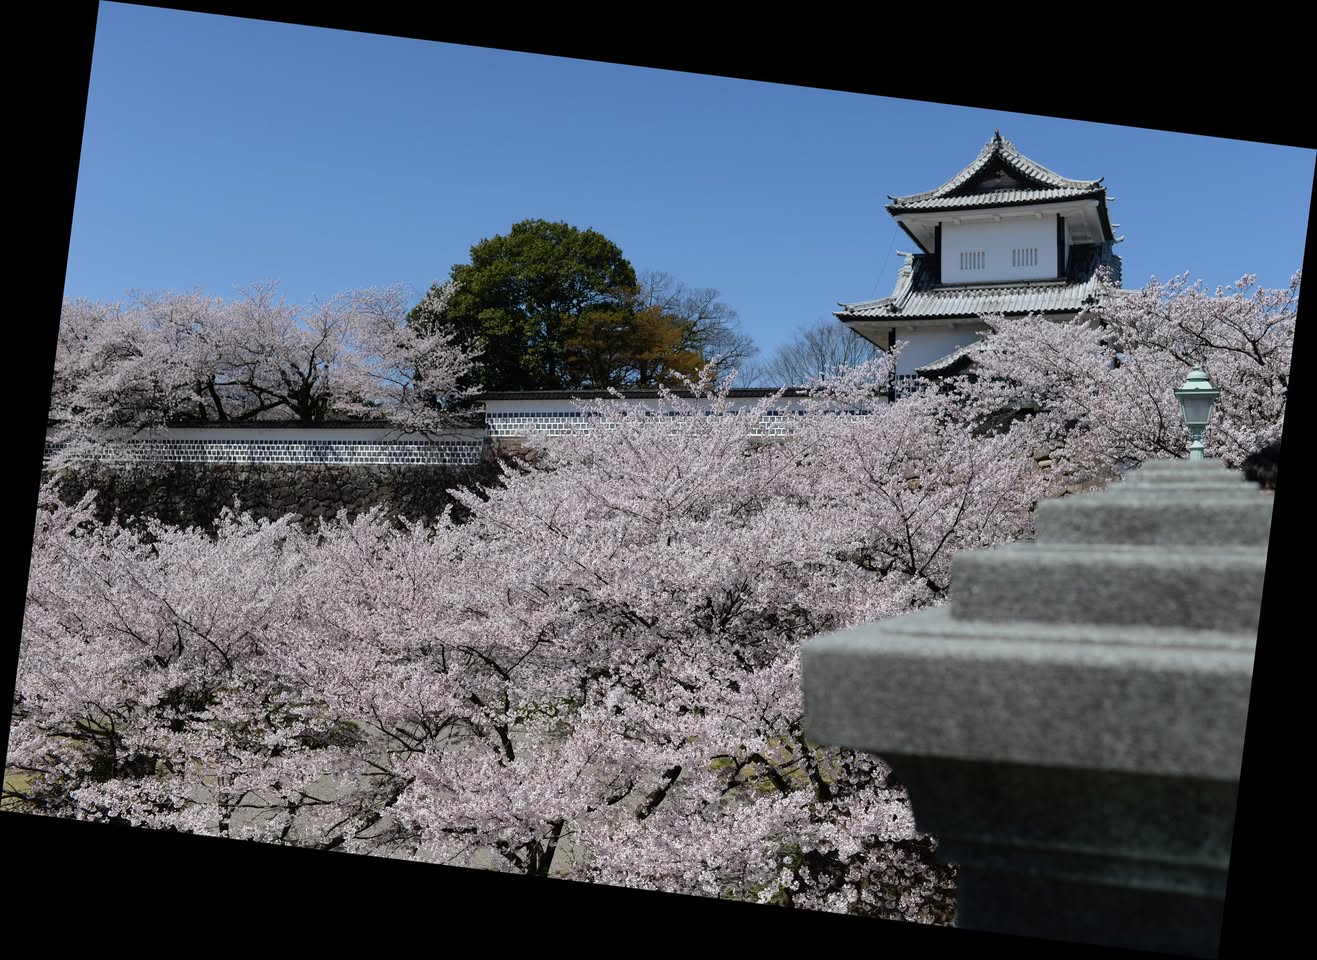
\includegraphics[width=\linewidth]{pictures/2024/04/20240410_133651_001.jpg}
\end{minipage}
\end{center}

\section{5月}

\subsection*{2024年05月01日 01:33}
\addcontentsline{toc}{subsection}{2024年05月01日 01:33}

\url{https://youtu.be/KHwsHXtVWks}

\begin{center}
\href{https://youtu.be/KHwsHXtVWks}{
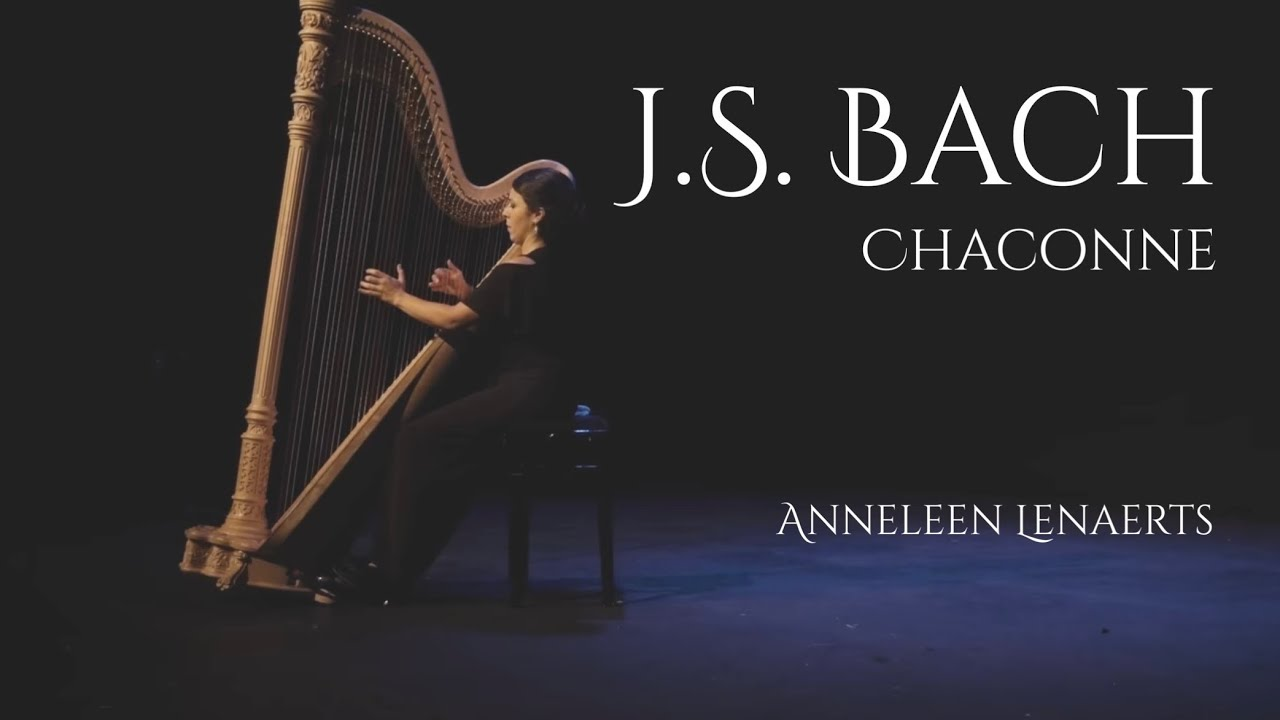
\includegraphics[width=0.48\linewidth]{pictures/youtube/2024/05/20240501_013357_youtube_001_KHwsHXtVWks.jpg}
}
\end{center}




美しい！

複数の声部が聞こえる（ポリフォニーって言うのかな)。あそこのアーティキュレーションはそんな風だったのか、という様な新しい発見がある。フレージングも新鮮に感じる（清少納言を清・少納言、択捉（え・とろふ）島と言うみたいな）部分がある。フレージングに合わせたアゴーギクの表現（というかルバート）がとっても素敵だ（私のテンポとピッタリ合っている気がする）。高音部でのダイヤモンドダストの様なppアルペジオからのディナーミクにも繊細さを感じる。そもそも分散和音がとても良い響きを聞かせてくれているのは、曲の出だしから既に感じられていたことだ。６弦ギターの演奏では聞こえていなかった音が随所に聞こえる様な気がする。ギターの弦の数がハープに比べて少ないからなのか？と思った直後、そもそも原曲は弦４本のバイオリン独奏曲だったことを思い出した。バイオリンという楽器も凄いことなのだが、作曲者大バッハも（言わずもがなだが）凄い！（結局ここに落ち着くのか）。「すごい」とか「うつくしい」とか、そんな感想しか思いつかない。


（ただ、実は曲の終わりの辺りで２箇所ほど数小節飛ばして演奏されている所がある？様な「気がする」。私の様な素人が「そんな気がした」というだけのことだが、編曲によって生じている違和感なのか、或いは私がこれまで聞いてきたものと演奏に使われている楽譜の版が異なっているのか、はたまた、、、演奏ミスの部分をビデオ編集時にカットしてごまかそうとした形跡なのか？）

\subsection*{2024年05月17日 20:20}
\addcontentsline{toc}{subsection}{2024年05月17日 20:20}

四月中頃から五月の中頃までの期間でしたが、新入社員を対象とした研修に、\#C言語 の \#オンライン講師 として加わりました。受講生は150人程。\#zoom による \#オンライン研修 なので、南は九州から北は北海道まで、全国の支店のフレッシュマンが受講した研修会でした。毎日の研修は業務ですから、9時から18時までキッチリ確保されています。ゴールデンウィークも当然の事ですが、カレンダー通りです。1時間毎に10分の休憩となっていますが、10分の休憩って思いの外短いんだなあという感想です。コーヒー入れてたら飲んでる時間がありませんから。そして、一日中zoomに自分が撮影されているとなると居眠りもできません。案外ハードだったという気がします。（受講者の方が大変なんだろうけど）


そもそもこれだけの人数を対象とするzoomによる研修って、本当に成り立つものなのか？最初は懐疑的に斜に構えていました。しかし、企画している会社の周到な準備の賜物なのか、十分に成り立つ研修形態なのだと分かりました。課題のプログラムを実際に入力して、動かしてもらいながら動作を確認しつつ進めていくのが主なスタイルでした。できた人はzoomの挙手の仕組みで人数を確認して進められていました。しかも、この研修は理解が及ばないで遅れがちな受講者に対しても、他の講師が（zoomのブレイクルームのしくみを使って）個別に対応して、（なるべく）落ちこぼれを出さない事を目指して運用されていました。（しかし、やっぱりC言語ではポインタが一つの越えるべき山場なんですよね）


一緒に関わった他の講師の方々とも、ティームとしてオンライン授業に取り組む事ができて、この年にして面白い新しい経験をする事ができたなあという感じです。終わったら、ちょっと寂しい様な気にもなりましたが、再び気楽な日々に戻るという事で、散歩にでも行くかなという気持ちでいますよ。

\subsection*{2024年05月18日 00:58}
\addcontentsline{toc}{subsection}{2024年05月18日 00:58}

\#金沢 は、\#犀川 と \#浅野川 の二つの川が流れていて、それぞれが \#河岸段丘 を削り出しており、二つの川に挟まれた部分が \#小立野台地 と呼ばれる高台になっています。このため、小立野台地に立つとそれぞれの川に向かって、両側に降りる「坂」が多いです。


さて、以下は最近（ここ１ヶ月ほど）私が「歩いて」みた坂道を、思いつくまま列挙してみました。少し健康になった様な気がしています。これらの坂がどこにあるかご存知でしょうか？歩いたことありますか？私の様な新参者にとっては、とても興味深い所です。


(１)\#紺屋坂

(２)\#廣坂

(３)\#兼六坂

(４)\#ハ坂

(５)\#旭坂（牛坂と勘違いしていた）途中 \#野坂 もあるらしい

(６)\#馬坂

(７)\#嫁坂

(８)\#新坂（\#小立野新坂、\#笠舞新坂 とも）

(９)\#白山坂

(１０)\#二十人坂

(１１)\#亀坂（ガメと濁って読みます）

(１２)\#鶴間坂（昔は \#牛坂 だったらしい）

(１３)\#大乗寺坂（お寺は野田山墓地辺りで、坂は \#本多の森 近く）

(１４)\#善光寺坂

(１５)\#木曽坂

(１６)\#天神坂（小立野トンネルができる前は、主要道路だった？）

(１７)\#あかり坂

(１８)\#暗がり坂

(１９)\#いもり坂（昔は \#宮守坂 (ミヤモリ坂)と読んでいたと思う）

(２０)\#甚右衛門坂

(２１)\#W坂 ( \#石伐坂 \#清立寺坂 \#吹屋坂 \#くの字坂 )


\#寺町 側から \#犀川 方向に降りてくる坂もあれこれある様だけど、（不吉な）W坂以外殆ど訪れていません。またネット上にはこれ以外のものも紹介されている様ですし、坂にまつわる文豪の話や歴史上の名前の由来など、面白いものがあったりするみたいなので楽しみは尽きません。

今日も天気がよさそうだし、どこの坂に行こうかな。

\section{6月}

\subsection*{2024年06月21日 21:19}
\addcontentsline{toc}{subsection}{2024年06月21日 21:19}

\url{https://x.com/sakura_med_dsci/status/1805442624939344001?s=61&t=5VtsOkpki6juEjPXsBq8hg}




p値について、昔から気になっていました。

仮説検定（主張したい事の逆を仮定して、その仮定を否定する）の話


リンク先の参照させて頂いた記事では、Rで試行されていたのですが、その記事を見ていて何となく分かった（？）ような「気がした」ので、お勉強だと思ってPythonでプログラムしてみた。


頭の中でイメージしているのは、それぞれ40人のA教室とB教室で、平均点50点、標準偏差10点の同じテストを実施。プログラムでは両方のクラスのテストの点数の「平均点の差」を求めるという事を10000回試行して、その（平均点の差の）分布を見ています。


ある先生があみ出した（画期的な）指導法をA教室で実施して確認テストをした所、A教室の平均点がB教室より2.5点良かったとします。その2.5点差ってその先生の指導法による効果があったからだと言っていいのか？


差がない（有意差無しの）両クラス（同じ学年から無作為に抽出された生徒たち）の間で同じテストを実施した場合でさえ、平均点の2.5点差って「よくある話」なんじゃないのかって言う事が、このシミュレーションによって定量的な値（確率）として知る事ができる。（今のシミュレーションの値では26.03％。4回に1回は、どちらかの教室の方が、平均点の差が2.5点より大きい値になる事が起こり得るんじゃないのか？）


それじゃあ何点以上の差があったら、その先生の指導法による効果が現れたと言っていいのか（A教室とB教室には「有意な差がない」を棄却する事ができるのか）を決めているのがp値だという事なのでしょうか。


正規分布で平均から2シグマ（標準偏差の2倍）以上離れた事が起こる確率が約0.05である事（今のシミュレーションでは2シグマ以上は4.73\%）と関連があるのか？不明だけど、p値としてp=0.05が選ばれる事が多いらしい。実験物理の世界では5シグマ以上離れていないと有意差が有るとは言わない慣習だとの事（厳しい！5シグマって何パーセント？）。教育の世界ではどういう値なのだろうか？（多分5\%（両側合わせて）でしょう）


A教室を指導した先生の指導法の効果が見られたと言いたい場合、今のシミュレーションでは、平均点でB教室に概ね4.5点以上の差（2シグマ離した値）をつけていれば、「たまたまじゃなかったんだね」と言ってあげられるという事かな。

或いはもう少し面倒くさい説明をするならば、

A教室に何ら特別な指導をしていない状況（帰無仮説）で、B教室に対して4.5点以上の平均点の差がついた。この事が起きる確率は2.5\%(5\%の半分)未満（=>小さい確率=>ほとんど起きない事）=>ところが実際にその差が生じているとしたら=>それはきっと最初の「仮説」が間違っていたから（従って帰無仮説を棄却する）=>A教室に何らかの特別な指導があったから生じた平均点の差なのかもしれない。これは「p値2.5\%(p=0.025)で有意差の判定をしました」という事か。


平均点の差がプラスの場合をA教室がB教室より平均点が良かった場合、マイナスなのが逆にB教室の方が良かった場合、と見れば、ヒストグラムの右に2シグマ以上離れた部分の頻度と、左に2シグマ以上離れた部分の頻度がそれぞれ2.5\%ずつ、両側で5\%と見ればいいのかな。


そう言えば、学生だった頃「品質管理」という科目の集中講義が夏にあった。その時に帰無仮説だとか、棄却するだとかの言葉に出会っているんだけど、聞いたことあるというだけで身についていなかったんですね。（学生時代の事って、そういう身についていない事ばっかりだったな）


\#有意差 \#p値 \#正規分布 \#棄却 \#帰無仮説 \#Python \#統計

\paragraph{写真}
\begin{center}
\begin{minipage}{0.48\linewidth}
\centering
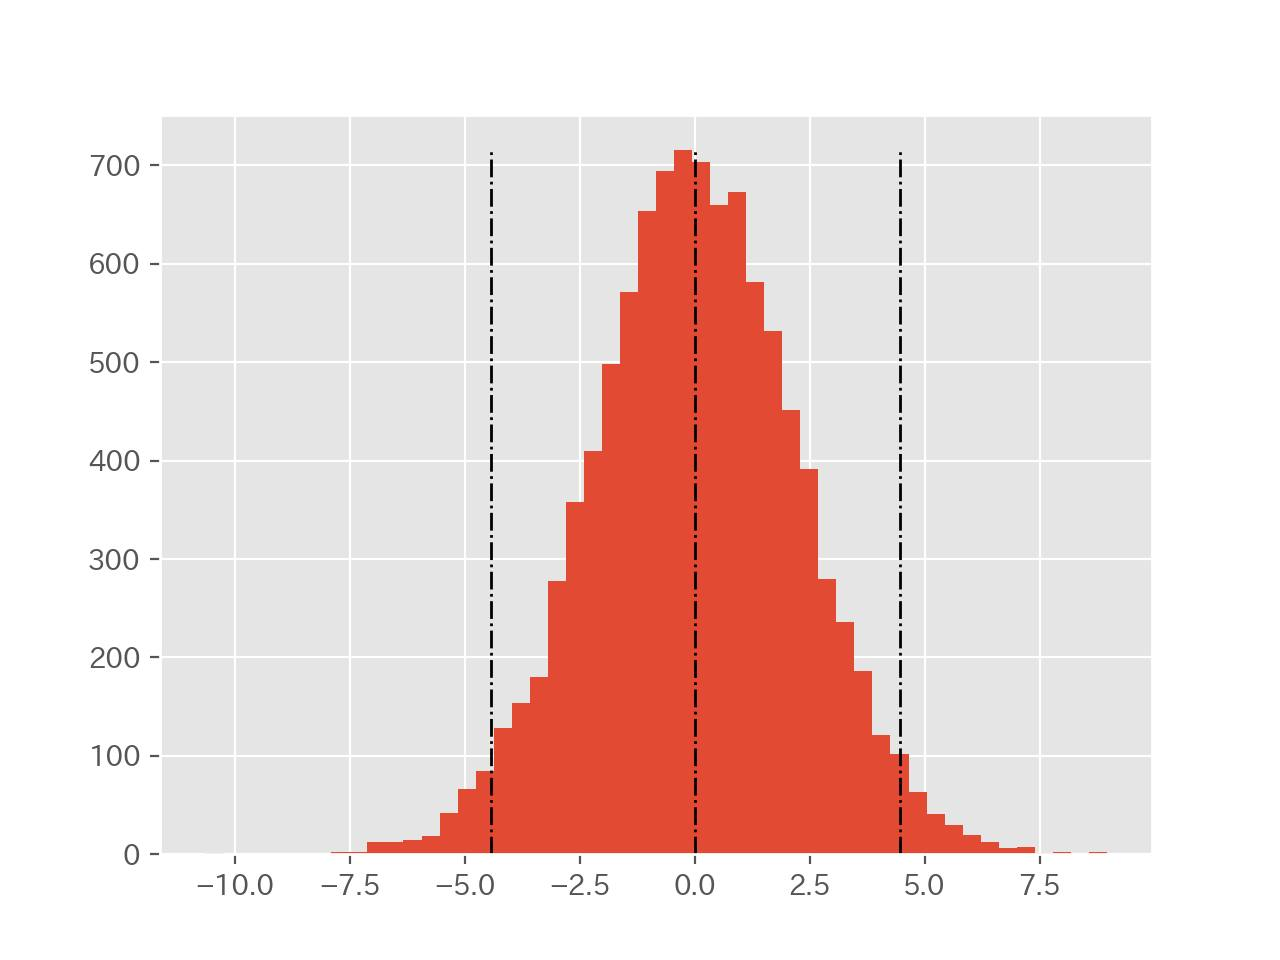
\includegraphics[width=\linewidth]{pictures/2024/06/20240621_211941_001.jpg}
\end{minipage}
\hfill
\begin{minipage}{0.48\linewidth}
\centering
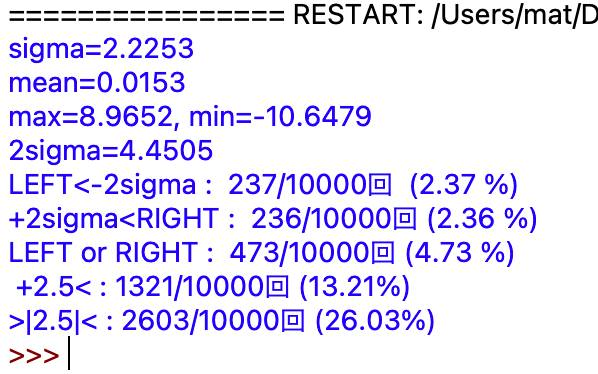
\includegraphics[width=\linewidth]{pictures/2024/06/20240621_211941_002.jpg}
\end{minipage}
\end{center}

\begin{center}
\begin{minipage}{0.48\linewidth}
\centering
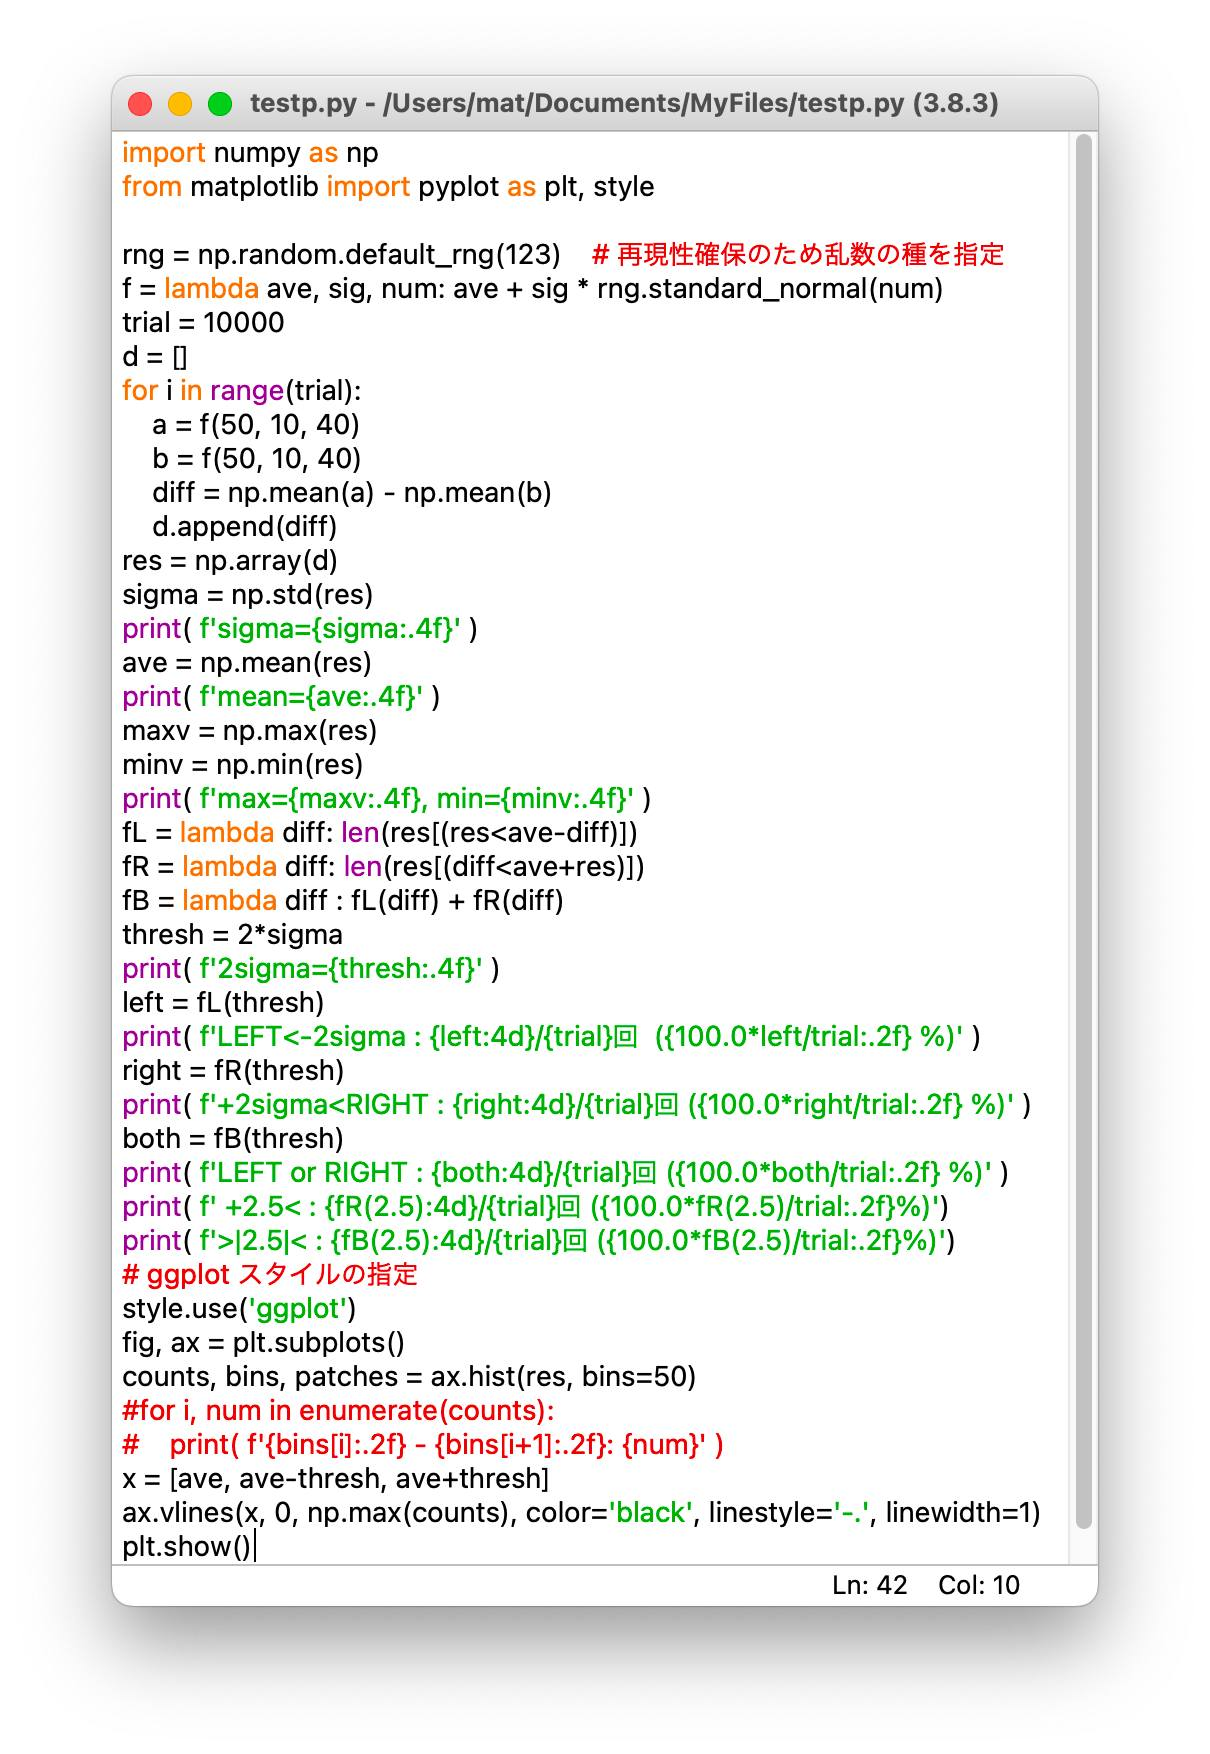
\includegraphics[width=\linewidth]{pictures/2024/06/20240621_211941_003.jpg}
\end{minipage}
\end{center}

\subsection*{2024年06月29日 04:09}
\addcontentsline{toc}{subsection}{2024年06月29日 04:09}

天気のいい日だったので、\#金沢 市 \#犀川 の散歩に出かけました。Apple Watchの記録によれば、約2時間半かけて距離7.4kmを歩いたようです。


\#大桑橋 から、\#犀川雪見橋、\#上菊橋、\#下菊橋、\#桜橋 と、順に 犀川 を川下に向かって歩きました。桜橋から更に川下に向けて \#犀川大橋 までは、\#室生犀星 が好んだ道として「\#犀星のみち」と名付けられている様ですが、体力的な理由から、桜橋までとしました。


大桑橋から \#犀川緑地 に入ると、芝生が植えられ、散策コースとして整備されています。途中、3羽の鴨？でしょうか？のんびり羽を休めているようでした。桜橋から \#寺町 に向かって登る \#W坂 の途中には、作家 \#井上靖 氏の「\#北の海」に、W坂に関する記述がある事が紹介されています。


W坂を登りきるとすぐ右手に \#本因寺 というお寺があって、ここのお寺には学生だった頃に宿泊したことがあります。本堂で雑魚寝だったと思いますが、朝になると、大きな声の読経が、木魚の音と一緒に鳴り響き、目覚ましになっていました。（1年生は木魚のすぐ近くに寝ていて、上級生は離れたところで寝ていた様な気がします。）

\paragraph{写真}
\begin{center}
\begin{minipage}{0.48\linewidth}
\centering
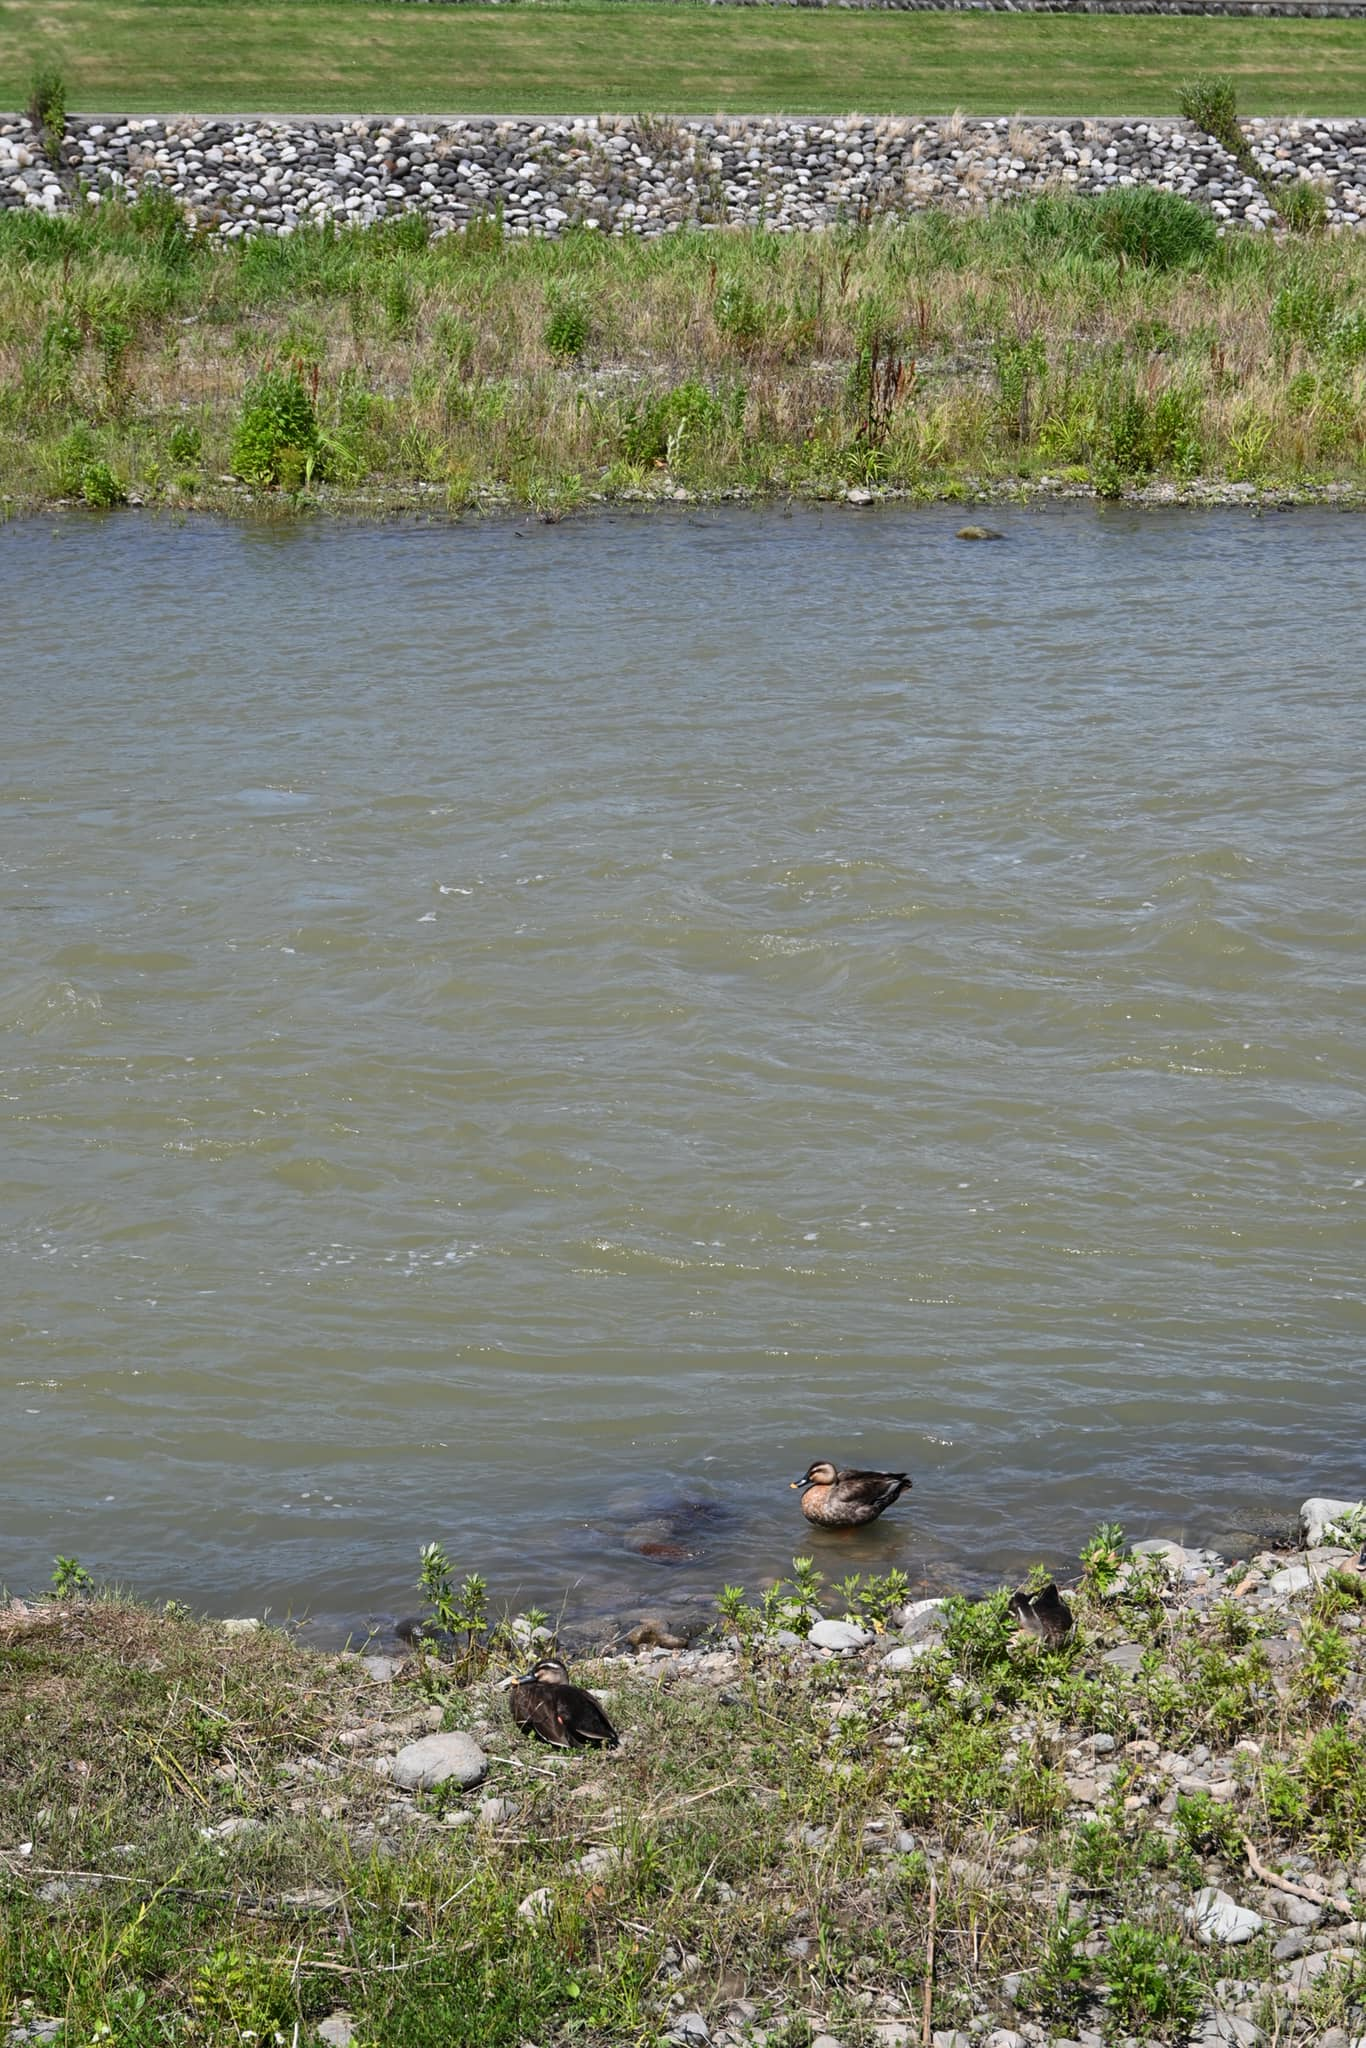
\includegraphics[width=\linewidth]{pictures/2024/06/20240629_040954_001.jpg}
\end{minipage}
\hfill
\begin{minipage}{0.48\linewidth}
\centering
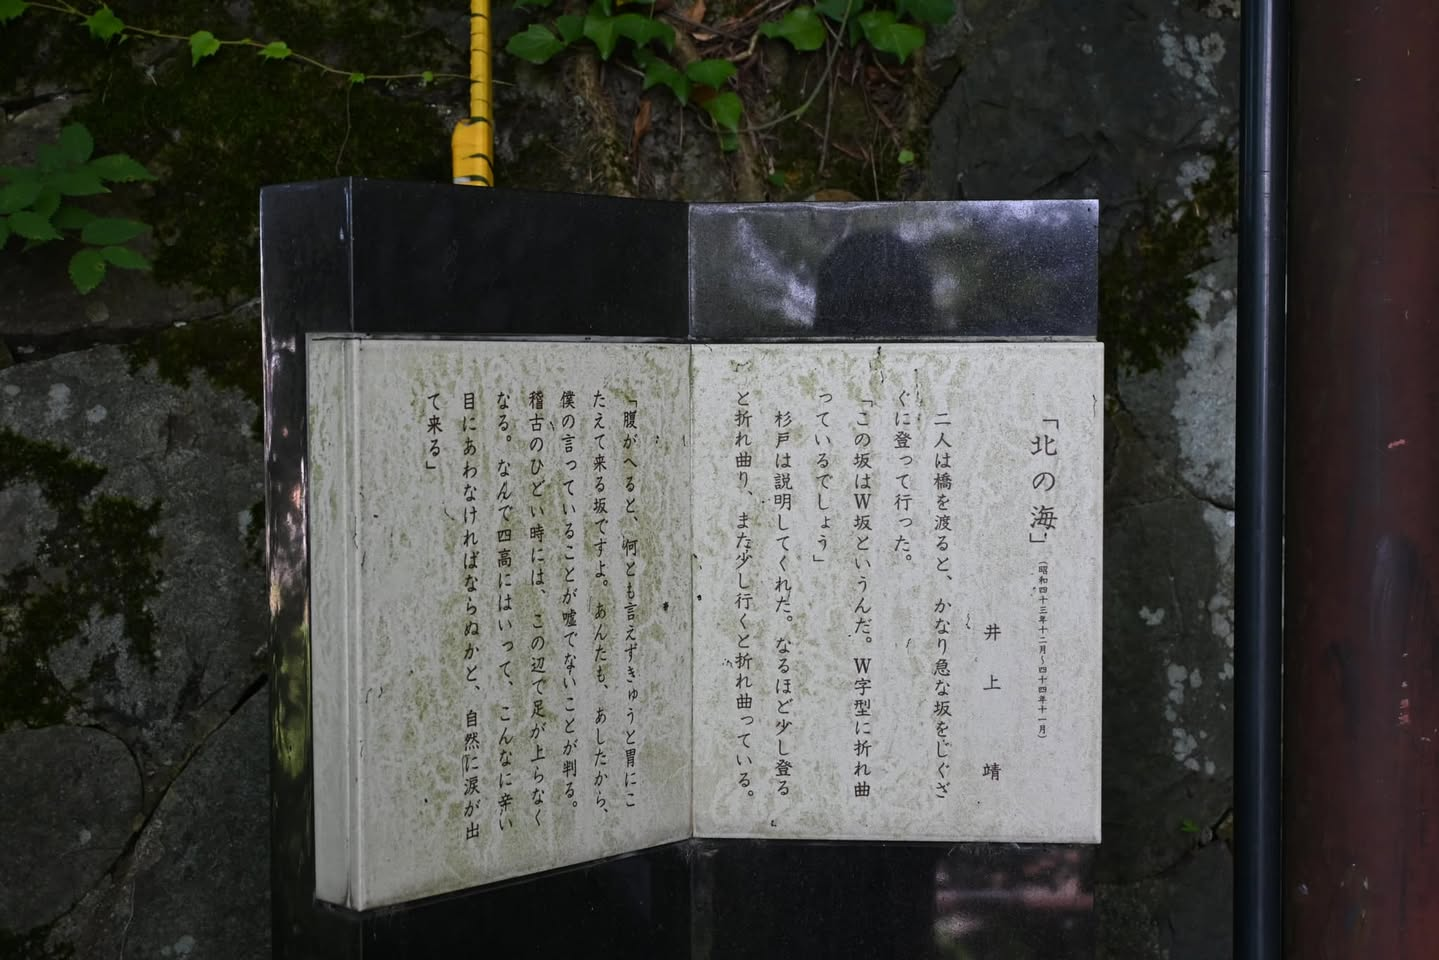
\includegraphics[width=\linewidth]{pictures/2024/06/20240629_040954_002.jpg}
\end{minipage}
\end{center}

\begin{center}
\begin{minipage}{0.48\linewidth}
\centering
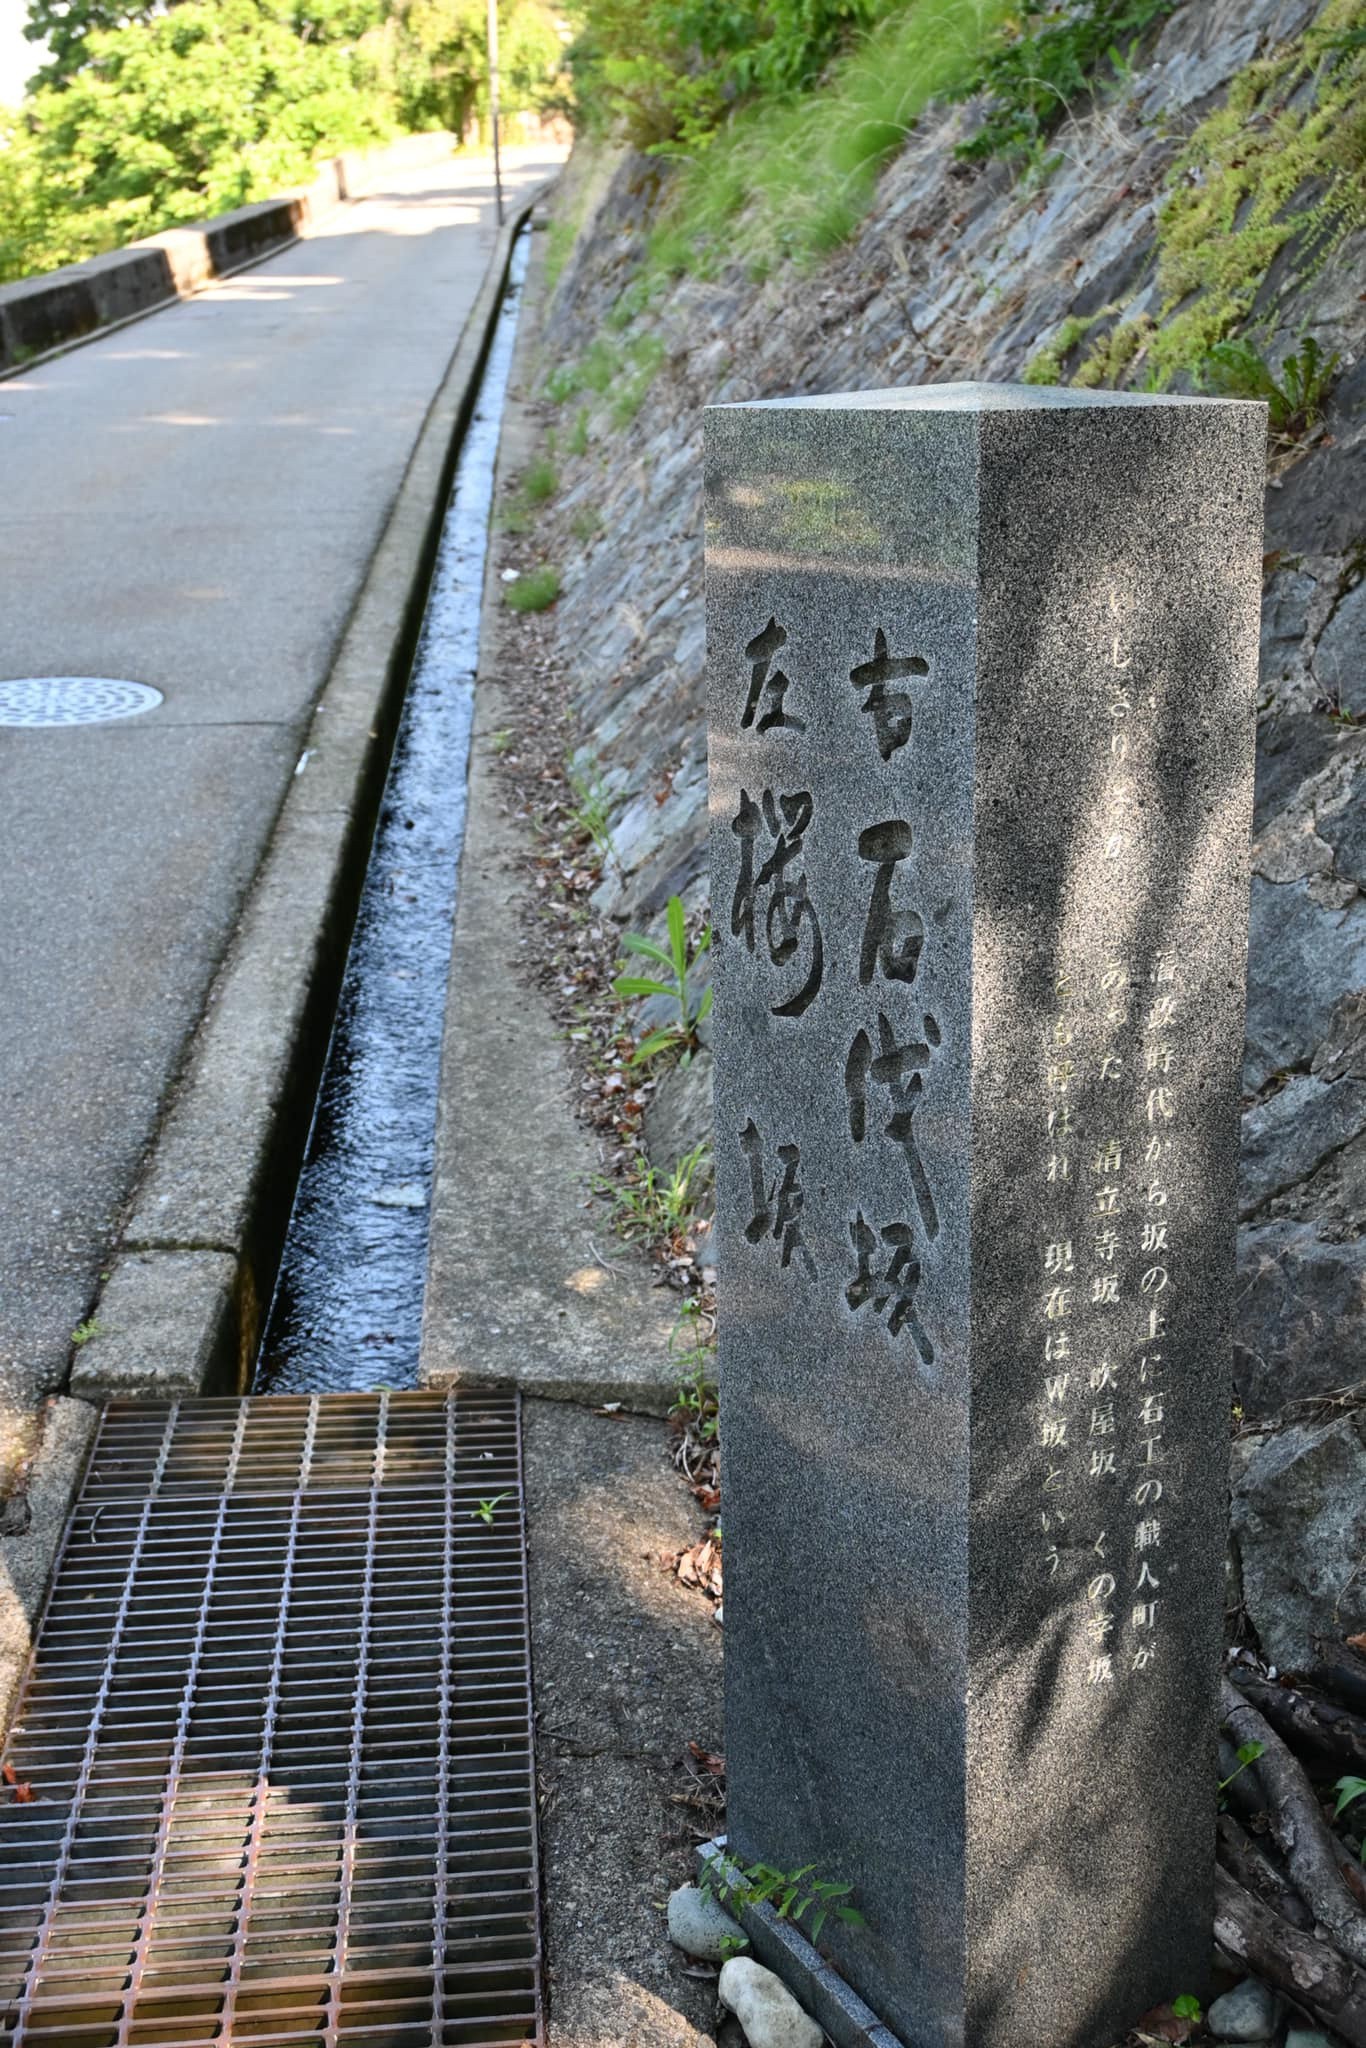
\includegraphics[width=\linewidth]{pictures/2024/06/20240629_040954_003.jpg}
\end{minipage}
\hfill
\begin{minipage}{0.48\linewidth}
\centering
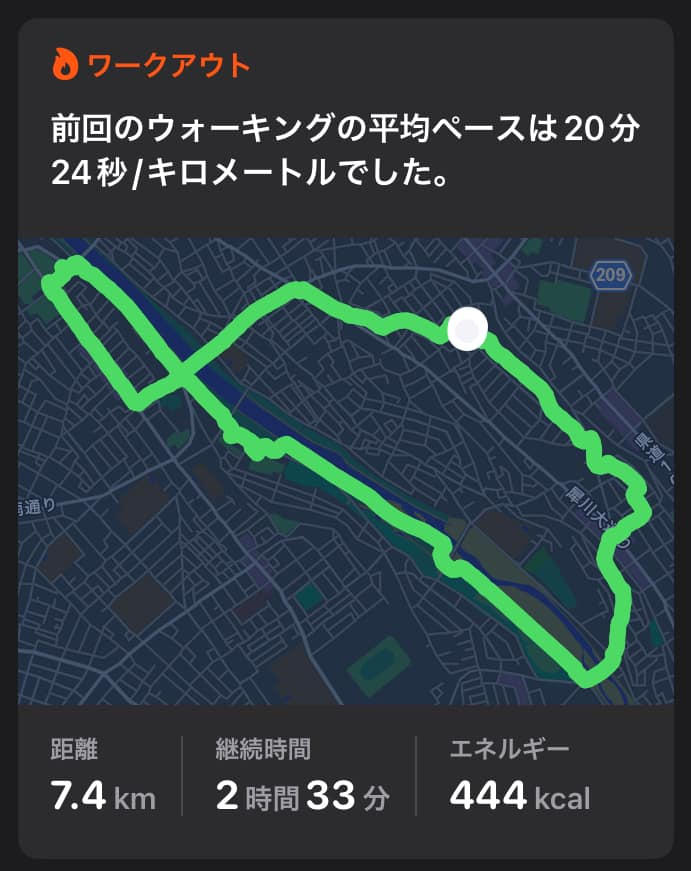
\includegraphics[width=\linewidth]{pictures/2024/06/20240629_040954_004.jpg}
\end{minipage}
\end{center}

\section{7月}

\subsection*{2024年07月02日 19:57}
\addcontentsline{toc}{subsection}{2024年07月02日 19:57}

\#金沢城 の \#玉泉院丸庭園 （廃藩時まで金沢城内のここ \#玉泉院丸 にあった庭園を再現したもの）で、庭園を整えていらっしゃる職人さんの姿です。背中に書かれた「\#兼六園」の文字！これをまとう事ができるのは石川県内に僅か７人。技術を持った職人として選ばれた方の証（あかし）なのだそうです。


\#玉泉院 は、\#織田信長 の五女で \#加賀藩 二代目藩主 \#前田利長 の正室。三代目藩主の \#前田利常 は、玉泉院の死後に、\#西の丸 と呼ばれていたこのエリアを玉泉院丸と改め、庭園を造ったとの事です。玉泉院の供養塔と言われる五輪塔がある \#玉泉寺 は \#寺町 に現存するが、今では寂れた寺になっている。


奥に見える \#三十間長屋 の下を \#宮守坂（陸軍第九師団司令部がお城にあった頃に作られた坂道）が右手方向に下っていて、その坂の手前が玉泉院丸庭園です。この庭園部分は、その昔（昔と言っても \#金沢大学 がお城にあった頃のこと）物凄く暗い荒れた林の中で、ボロのプレバブ小屋があった場所です（そこで合奏練習をした事もありました）。その荒れた林を切り開いて現在の観光用の庭園として整備されている訳ですが、そこに、お城だった頃の立派な石垣（縦長の短冊状の石も含めて）が広がっていたことは、全く知りませんでした。そもそも森の様な林の中だったので何も見えなかった（無頓着で気付かなかった）し。


なお、\#鼠多門 を入ってすぐの所に観光客のための「玉泉庵」という休憩所が設置され、そこで抹茶を頂きながらゆっくり玉泉院丸庭園を愛でる事ができるようになっています。（ただ私が行ったタイミングでは、多数の外国人旅行客が利用されており「貸切」との事でした）

\paragraph{写真}
\begin{center}
\begin{minipage}{0.48\linewidth}
\centering
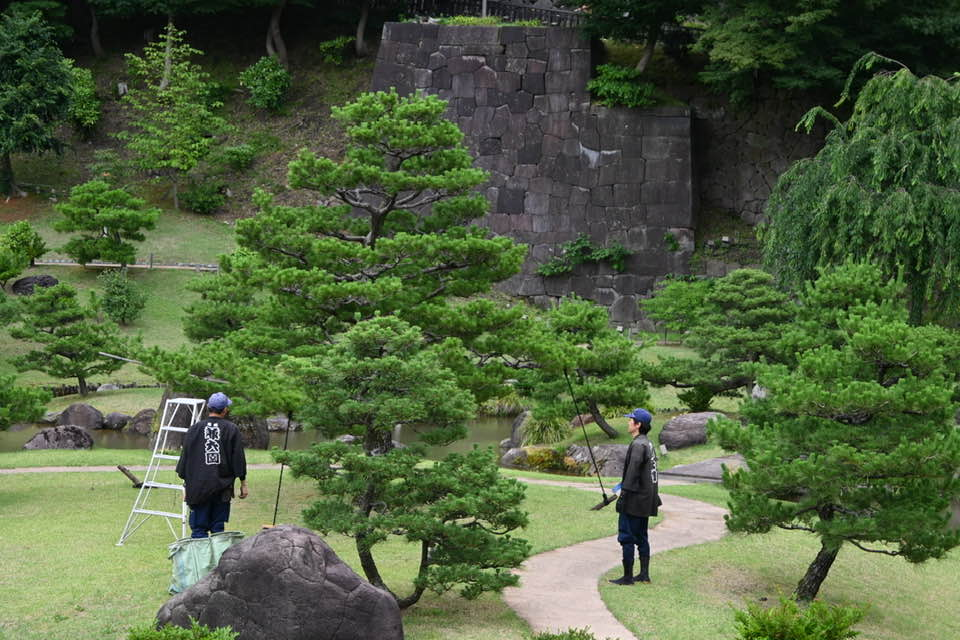
\includegraphics[width=\linewidth]{pictures/2024/07/20240702_195732_001.jpg}
\end{minipage}
\hfill
\begin{minipage}{0.48\linewidth}
\centering
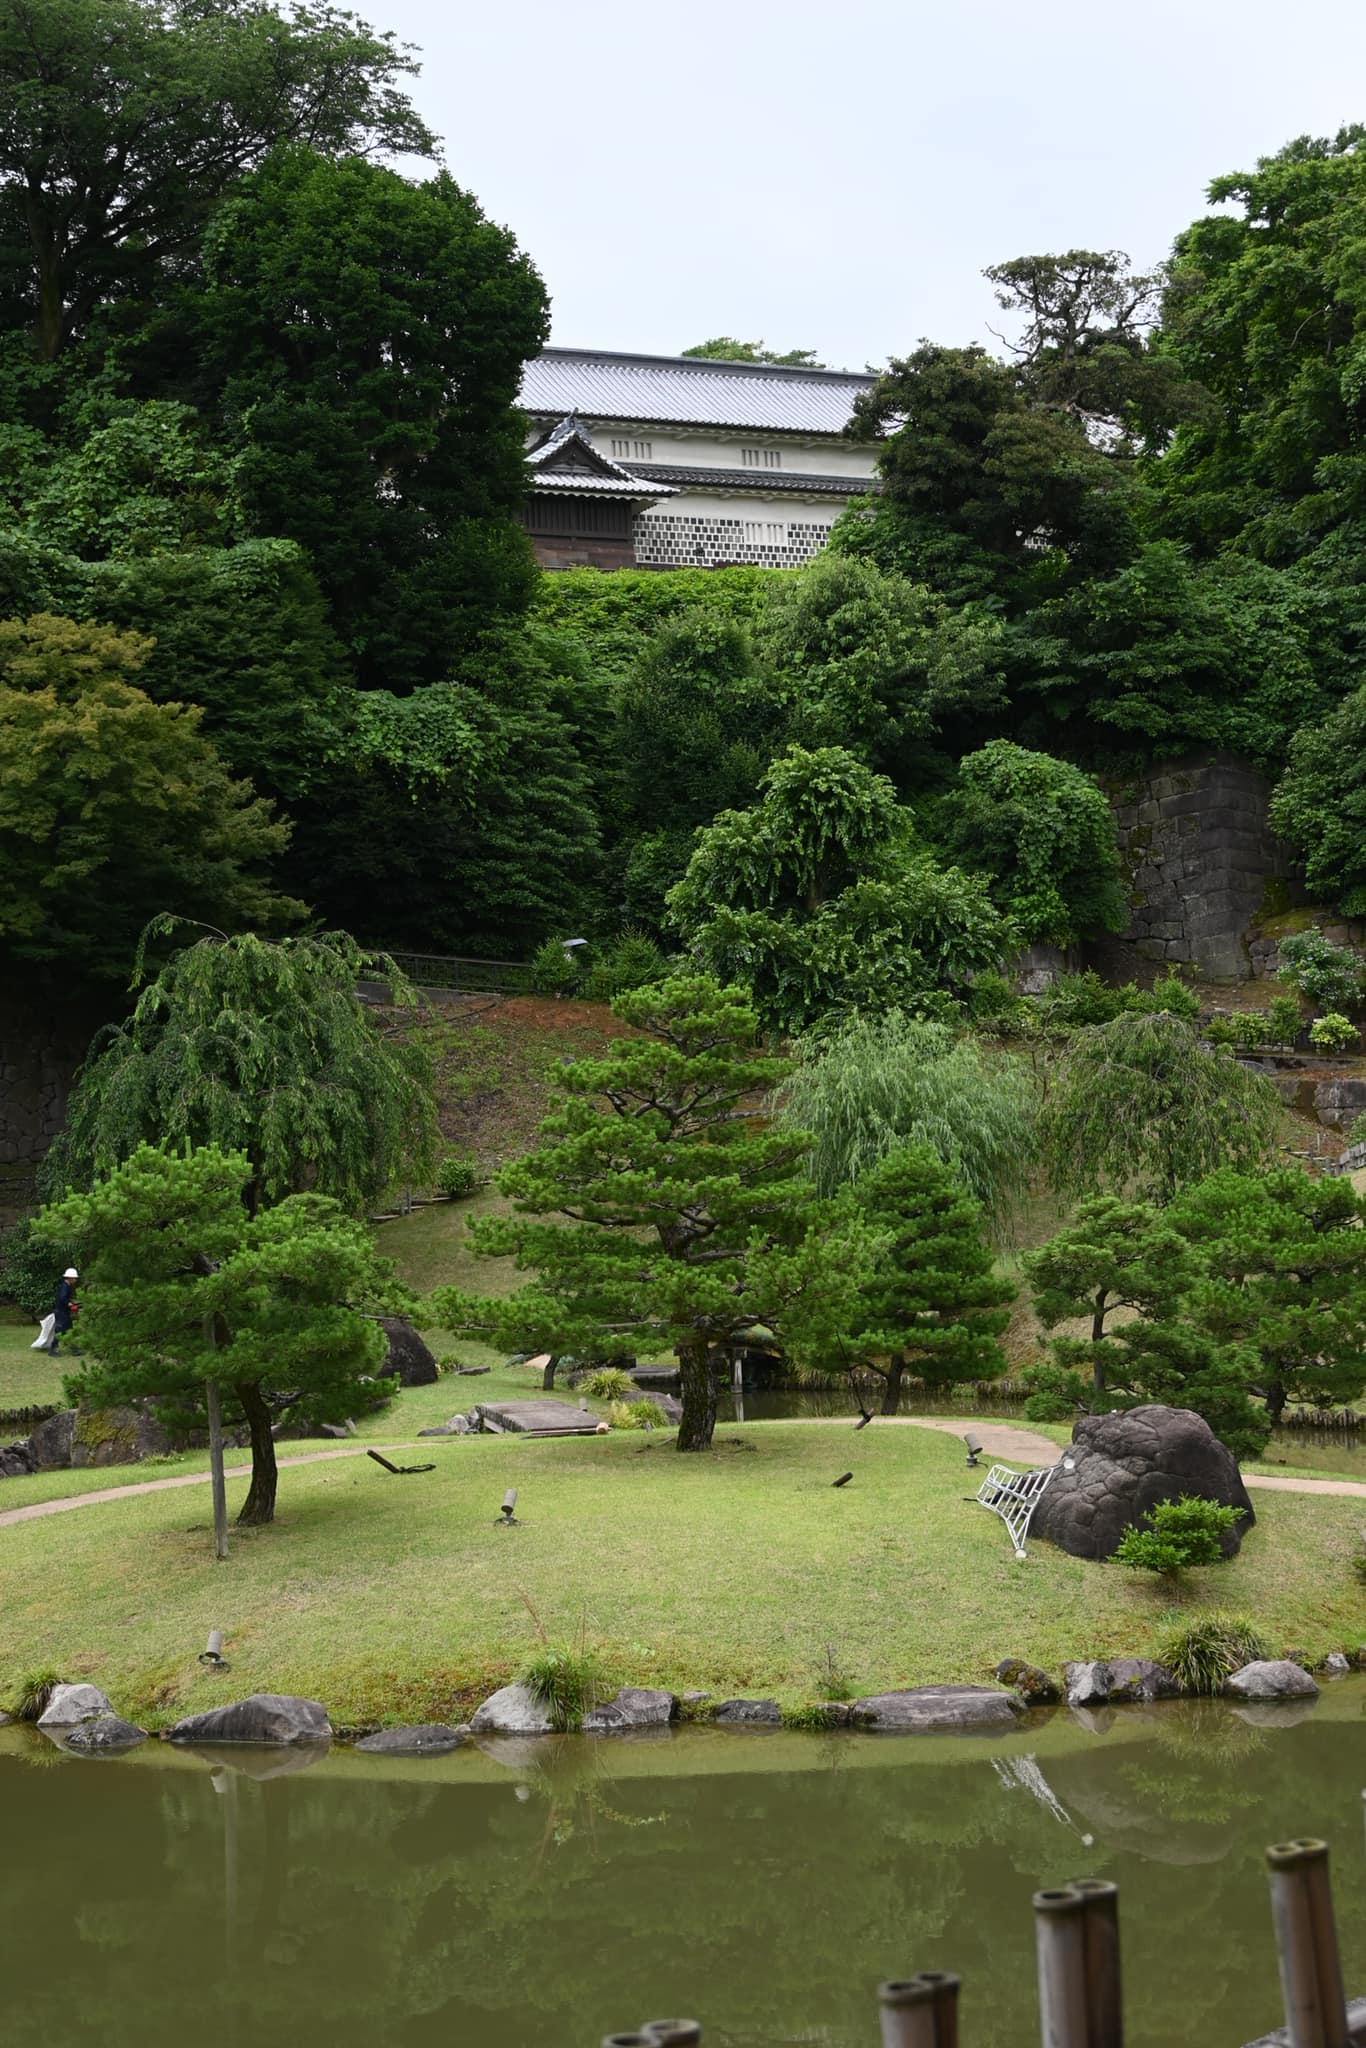
\includegraphics[width=\linewidth]{pictures/2024/07/20240702_195732_002.jpg}
\end{minipage}
\end{center}

\subsection*{2024年07月04日 01:34}
\addcontentsline{toc}{subsection}{2024年07月04日 01:34}

\url{https://m.facebook.com/story.php?story_fbid=7685108804906547&id=100002225117991}




p値について

Pythonでしたこと（上のリンク先）と同じことをRでも試してみた。

概ね同じ様な傾向を見せてくれていると思うけど、どうでしょう。

（値そのものがPythonの時と異なるのは、乱数の生成アルゴリズムとシードの両方或いはどちらか一方が異なっているから）

ところで、Rのシードはどうやって指定するのかな？（<-解決しました）


\#有意差 \#p値 \#正規分布 \#棄却 \#帰無仮説 \#統計 \#R

\paragraph{写真}
\begin{center}
\begin{minipage}{0.48\linewidth}
\centering
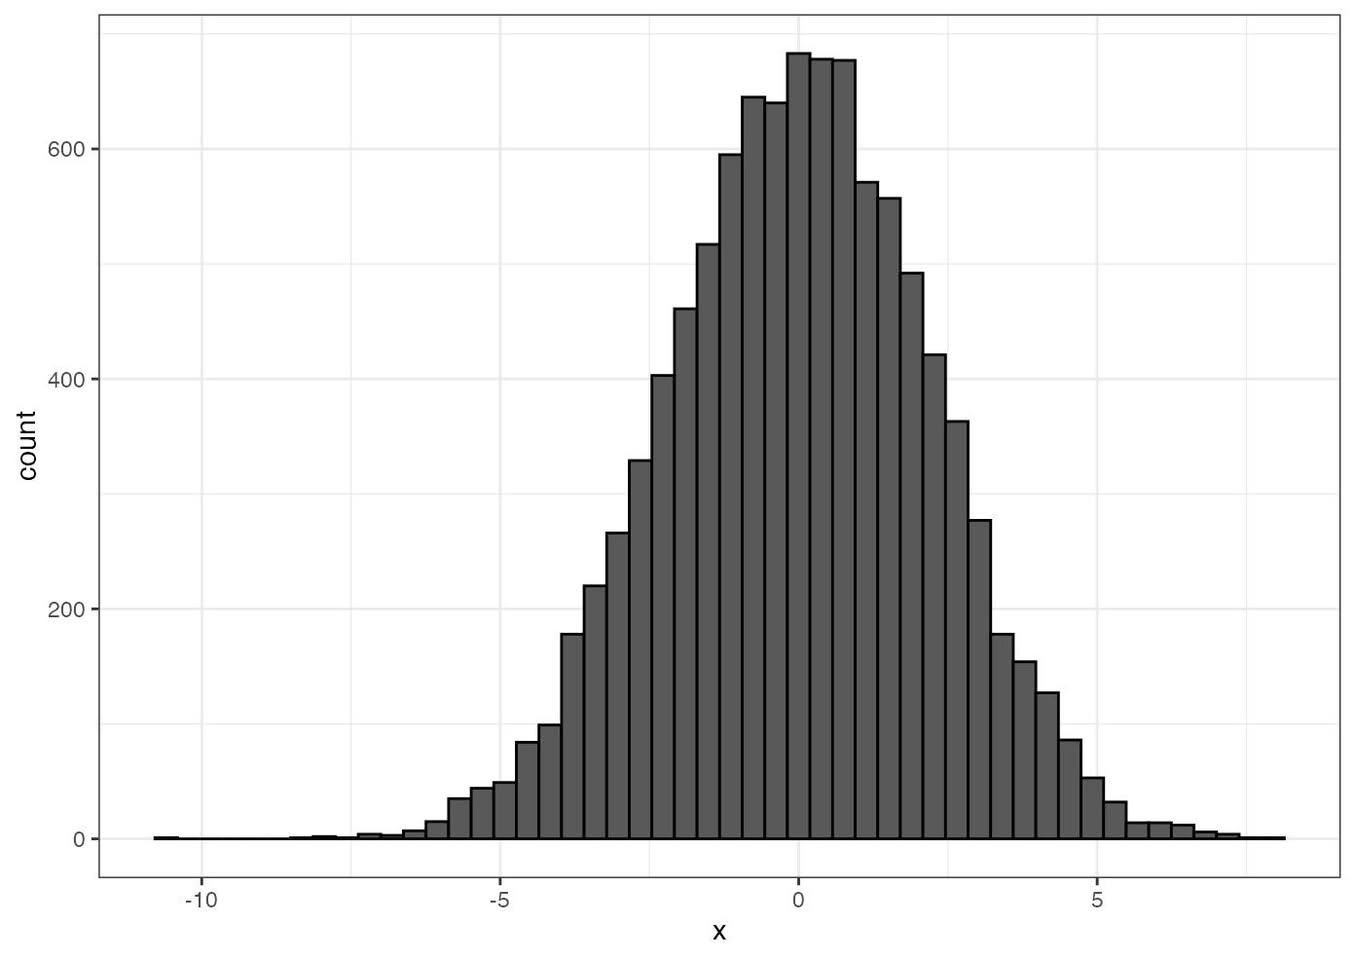
\includegraphics[width=\linewidth]{pictures/2024/07/20240704_013419_001.jpg}
\end{minipage}
\hfill
\begin{minipage}{0.48\linewidth}
\centering
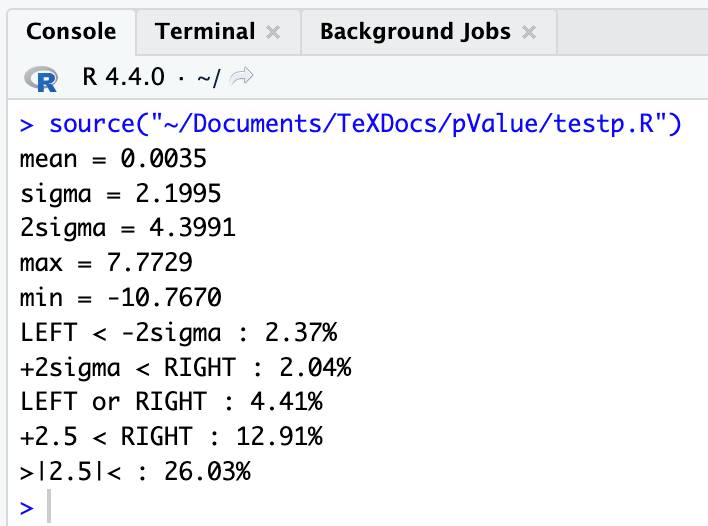
\includegraphics[width=\linewidth]{pictures/2024/07/20240704_013419_002.jpg}
\end{minipage}
\end{center}

\begin{center}
\begin{minipage}{0.48\linewidth}
\centering
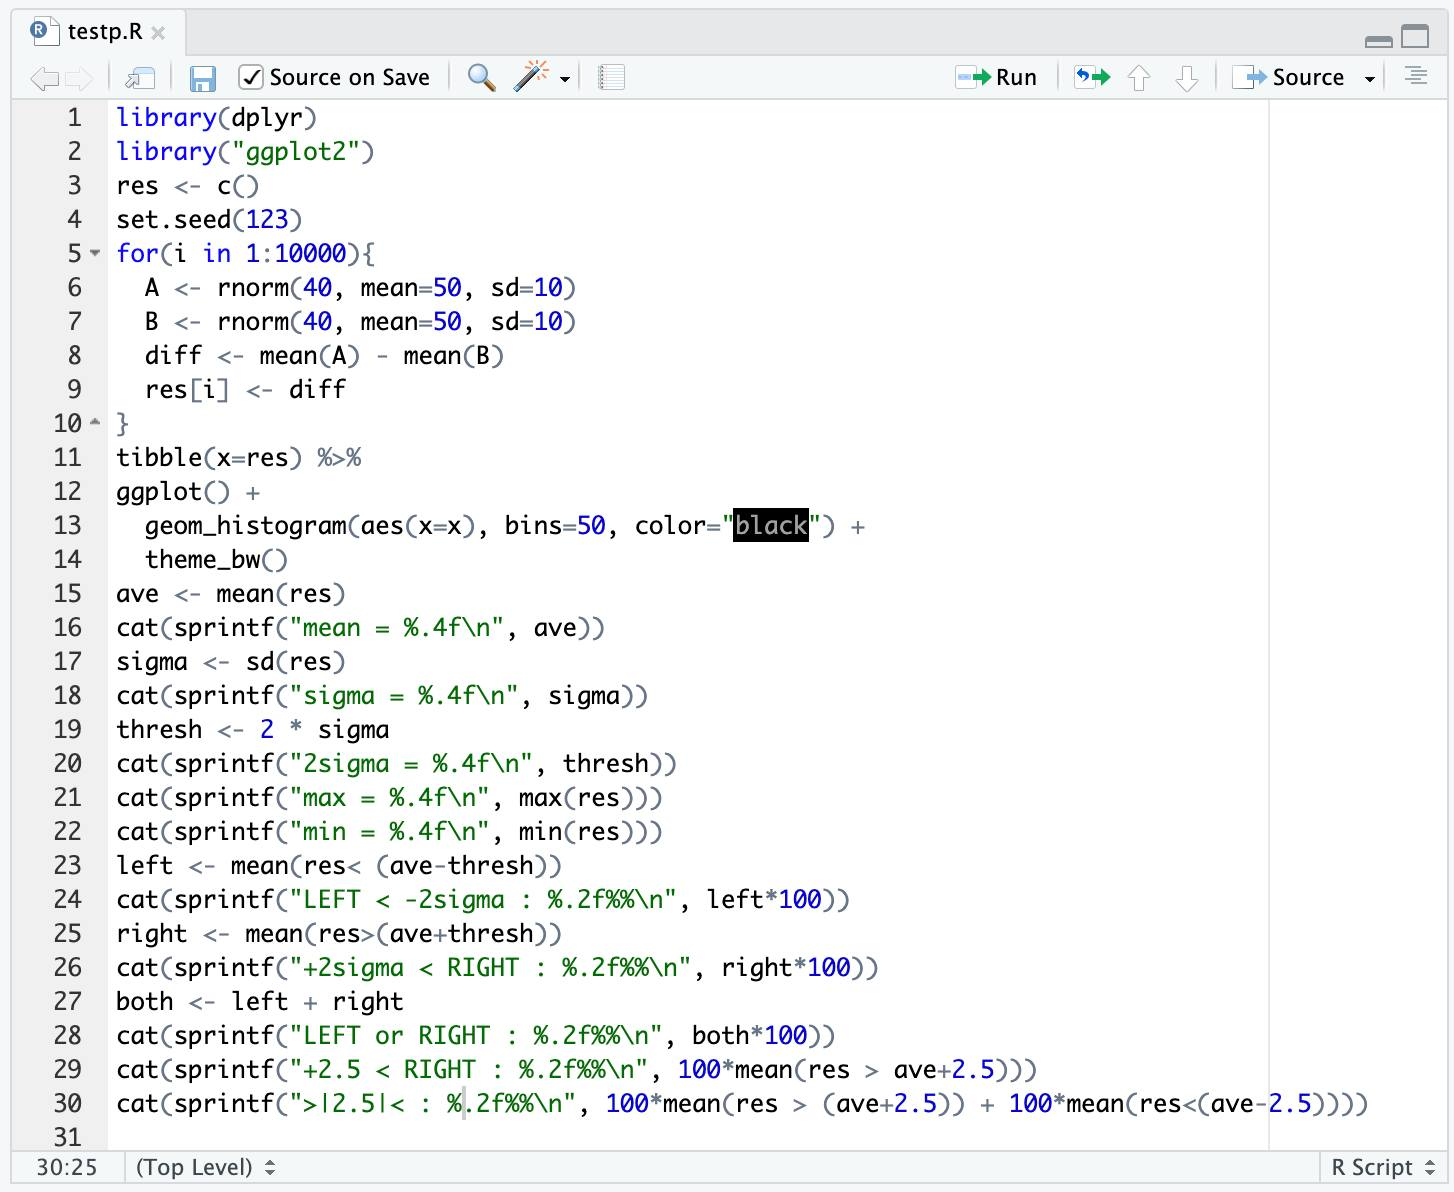
\includegraphics[width=\linewidth]{pictures/2024/07/20240704_013419_003.jpg}
\end{minipage}
\end{center}

\subsection*{2024年07月07日 19:42}
\addcontentsline{toc}{subsection}{2024年07月07日 19:42}

\url{https://m.facebook.com/story.php?story_fbid=26791557793776475&id=100000468522533}




人生の終わりに音楽がなっていてくれると素敵だと思う。何がいいだろうか？

フォーレのレクイエムでしょうか。(もう既にあの世にいってしまっているみたいです)モーツァルトのレクイエムでしょうか。（ラクリモサが終わったら、そこで静かに止めてほしい）いや、やはり大バッハでしょうか。神に捧げるのに恥ずかしくない曲をと生涯求めて止まなかった方ですから。すると、マタイ受難曲でしょうか。（と言いつつ、今まさに「憐れみたまえ」辺りがイヤホンから聞こえています）いや、そもそもどの曲も少々長すぎるかもしれません、、、

私が亡くなる時はBWV1034の第３楽章Andanteを枕もとで吹いてほしい、と以前、上の子にはお願いしていたんだけど覚えているだろうか。（手頃な長さですし）


などと弱気な事を考えていたところ、標記リンク先の記事を読んだ。「八十歳を自身のピーク」とは、芸の世界のプロフェッショナルは流石だと思います。自分のことを省みると、何をしたでもなく今日まで来たけれど、まだこの先十年ほどは生きているかもしれない、と思うようになりました。（トラベルソでBWV1034の第２楽章Allegroを納得してふけるようになれるだろうか。そのための練習時間は十分ありそうです。）（添付は私の愛聴盤の一つ）

\paragraph{写真}
\begin{center}
\begin{minipage}{0.48\linewidth}
\centering
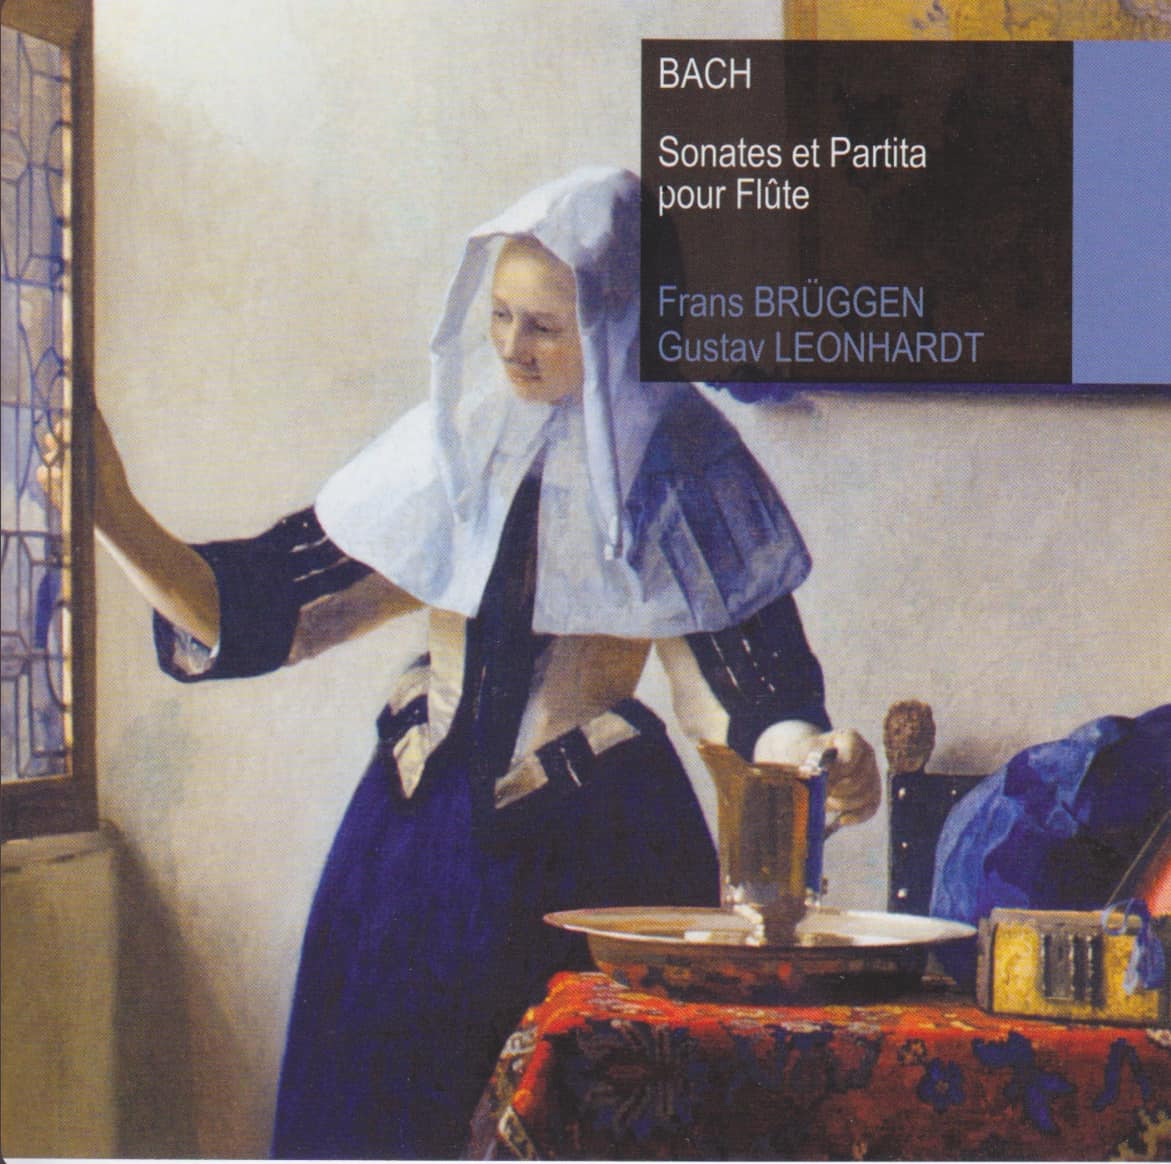
\includegraphics[width=\linewidth]{pictures/2024/07/20240707_194240_001.jpg}
\end{minipage}
\end{center}

\subsection*{2024年07月09日 01:03}
\addcontentsline{toc}{subsection}{2024年07月09日 01:03}

\url{https://x.com/shojihashimoto3/status/1810091468478103719?s=61&t=5VtsOkpki6juEjPXsBq8hg}




そう（熱は移動するエネルギーのこと）でしたか

「温度と熱を区別する必要がある」という事なのですね


熱は内から外へ移動したりするけど、温度は移動しない

温度は上がったり下がったりするけど、熱が発生したり消滅したりしたのではない


断熱圧縮は、断熱（外界との間で熱の移動がない）状態での圧縮（P→大）であり、温度Tは上がっても、それは熱が生じたのではない


摩擦で熱が発生したのではなくて、温度が上がった


ジュールの実験（水を攪拌したら、、）で、上昇したのは温度であって、熱が発生したのではない


運動エネルギーが熱エネルギーなるものに変わって、それが温度を上昇させるという考え方は普通に許されていた様な気がするんだけど、その考え方を許容しようとすると、熱力学の第二法則（温度差のなくなる方向に進む）がそれを許さないらしい。温度差がないと熱は移動しようがないし、熱の移動によって何らかの仕事をするという理解でしたが。（難しい話になってきた。もうこれでついていけてないわ。）


\url{https://www.jstage.jst.go.jp/article/butsuri1946/17/12/17_KJ00002736548/_article/-char/ja/}



（ここから切り抜いたけど、切り抜いちゃいけないんでしたっけ？同一性保持権？）

\paragraph{写真}
\begin{center}
\begin{minipage}{0.48\linewidth}
\centering
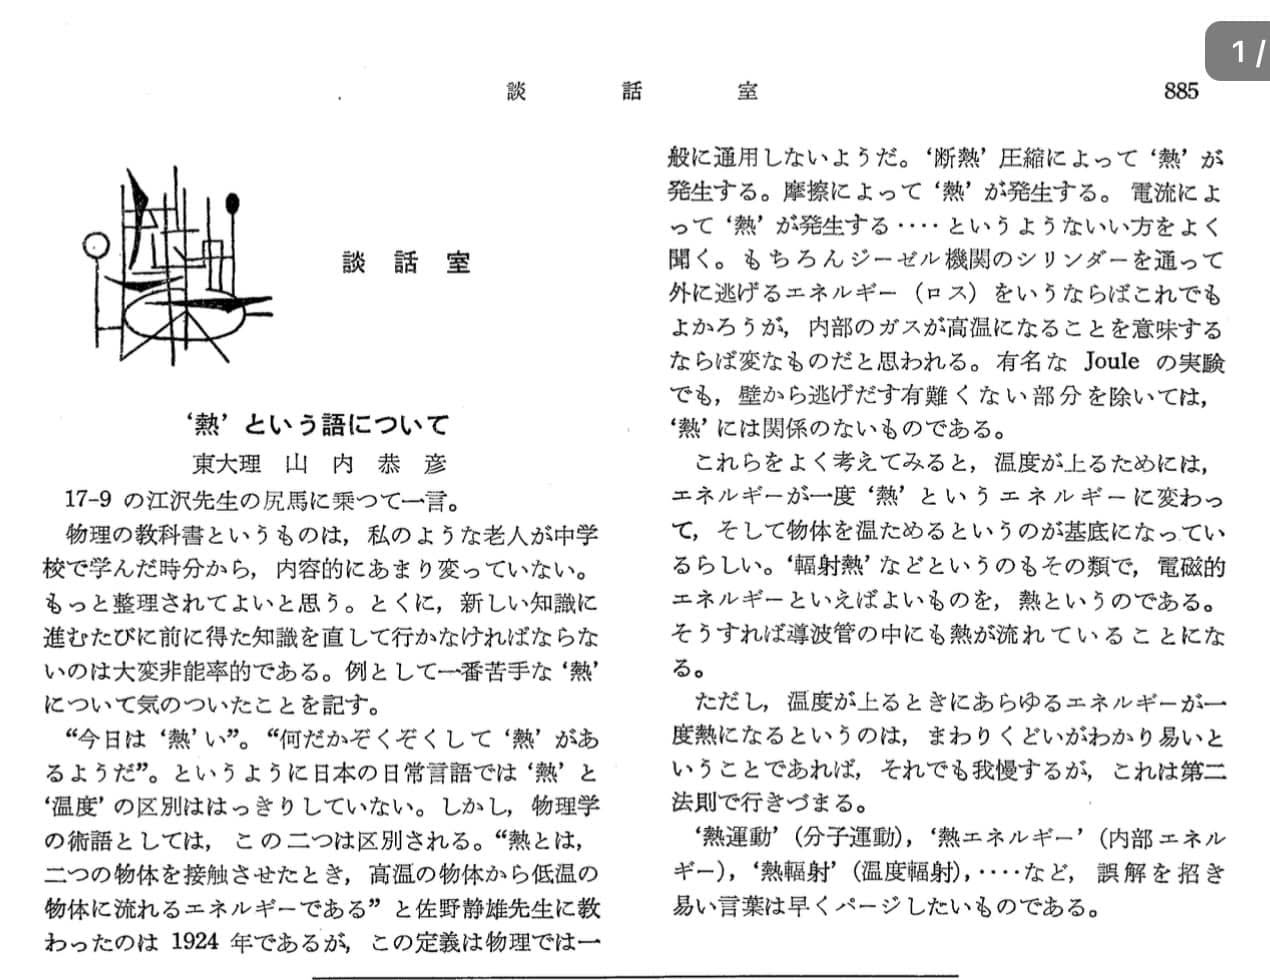
\includegraphics[width=\linewidth]{pictures/2024/07/20240709_010338_001.jpg}
\end{minipage}
\end{center}

\subsection*{2024年07月09日 14:40}
\addcontentsline{toc}{subsection}{2024年07月09日 14:40}

最近、英検二級や準一級が大学入試で利用されていると聞きます。立教大学や広島大学（難関の大学だという認識でいます）でも、英語検定の成績が入試に利用されているということです。私の時代には受験に関して英検は「out of 眼中」だったので、高校生が大学受験の対策として英検を受ける時代なのかと少し驚きでした。


高校生が準一級をとるのなら自分にも受かれるかもしれないと思って、対策本（添付画像の通り）を開いてみて愕然としました。とても歯が立つとは思えなかったからです。


でも「文単」はとてもよいですね。英文の長さは手頃ですし、取り上げられているトピックも興味深いものです。また、こんな言い回し、表現ができるのかという新しい発見が随所にあって、とても面白く読み進める事ができます。

また「英作文問題の完全制覇」ですが、(「文単」と違って)難しい単語や表現が使われているわけではありません。終始基本的な英文で記述されています。それにも関わらず本格的な難しいテーマについて論じることができている（これはすごい事）。感心してしまいます。この本を真面目に勉強したらきっと、英文で記述する力、作文する実践的な力を身につける事ができるんだろうなと思いました。

検定を受けなくても、いずれも読み物としてよい本でした。

\paragraph{写真}
\begin{center}
\begin{minipage}{0.48\linewidth}
\centering
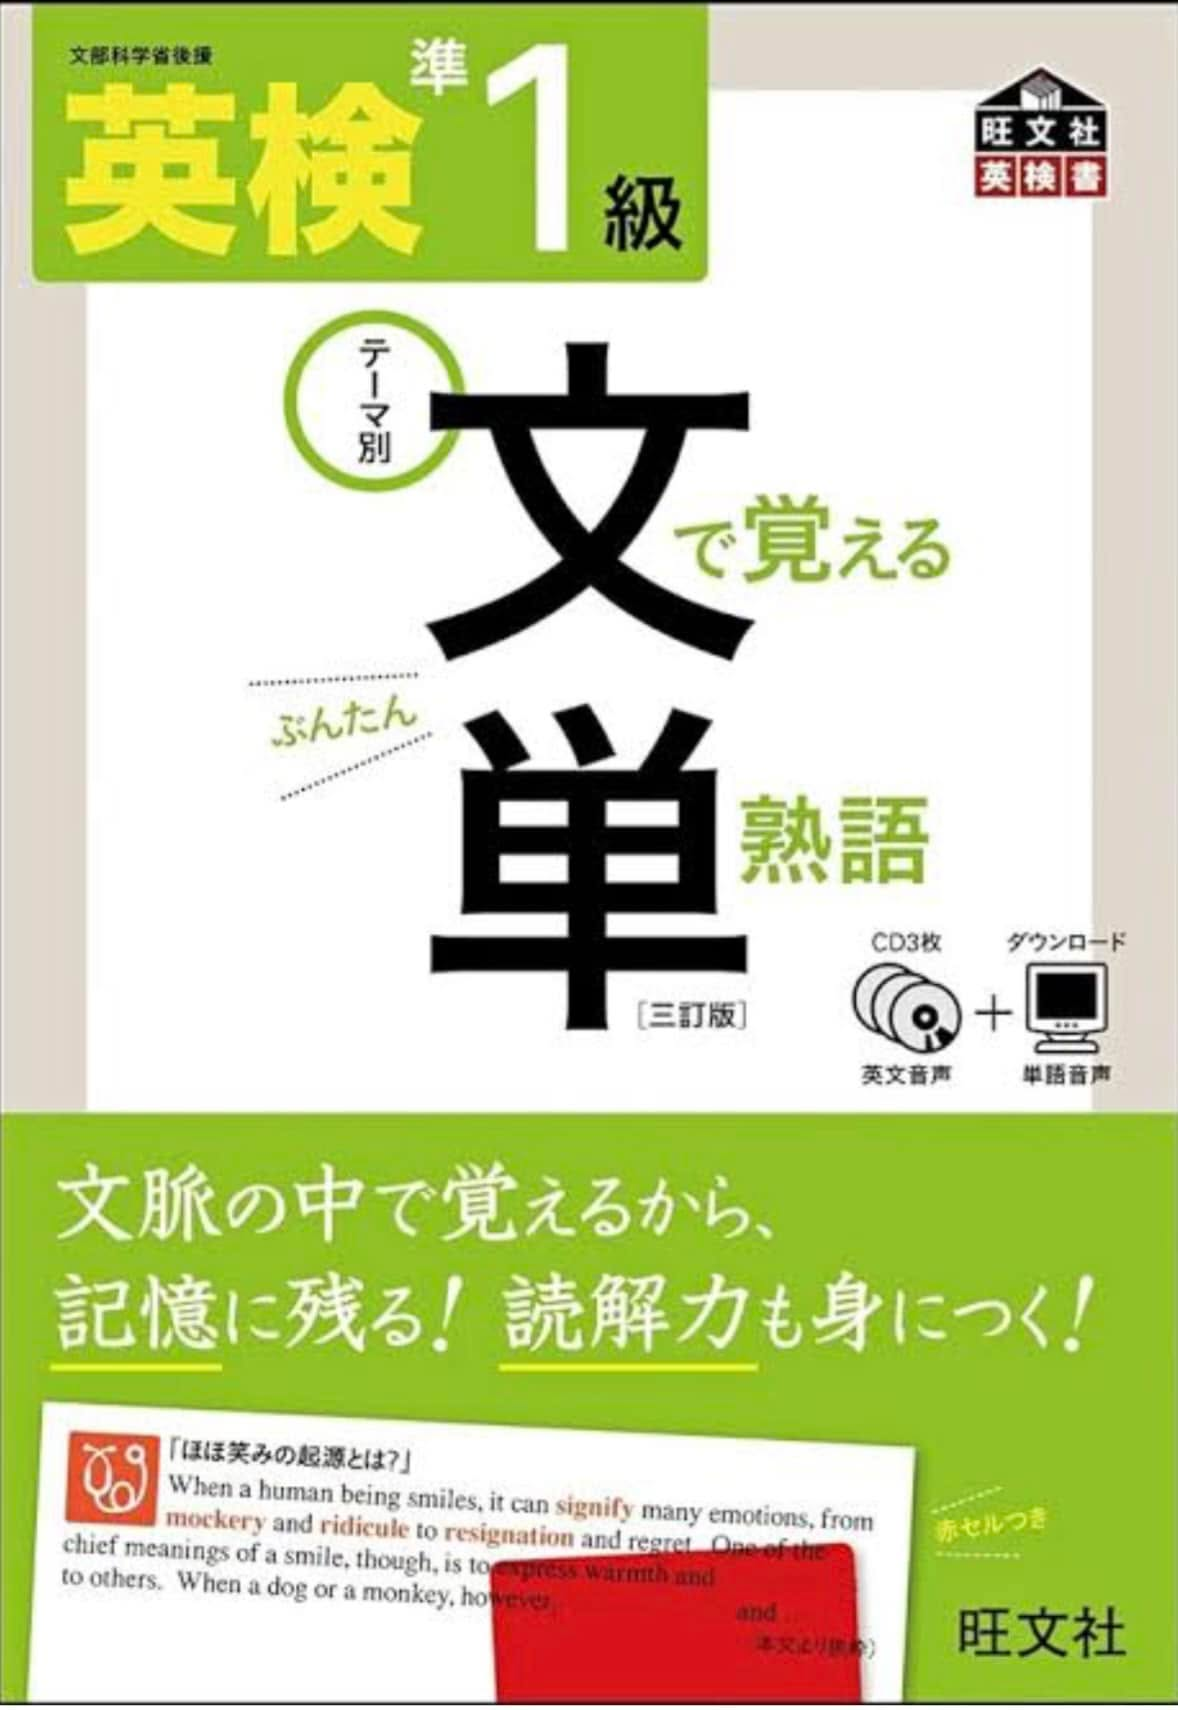
\includegraphics[width=\linewidth]{pictures/2024/07/20240709_144005_001.jpg}
\end{minipage}
\hfill
\begin{minipage}{0.48\linewidth}
\centering
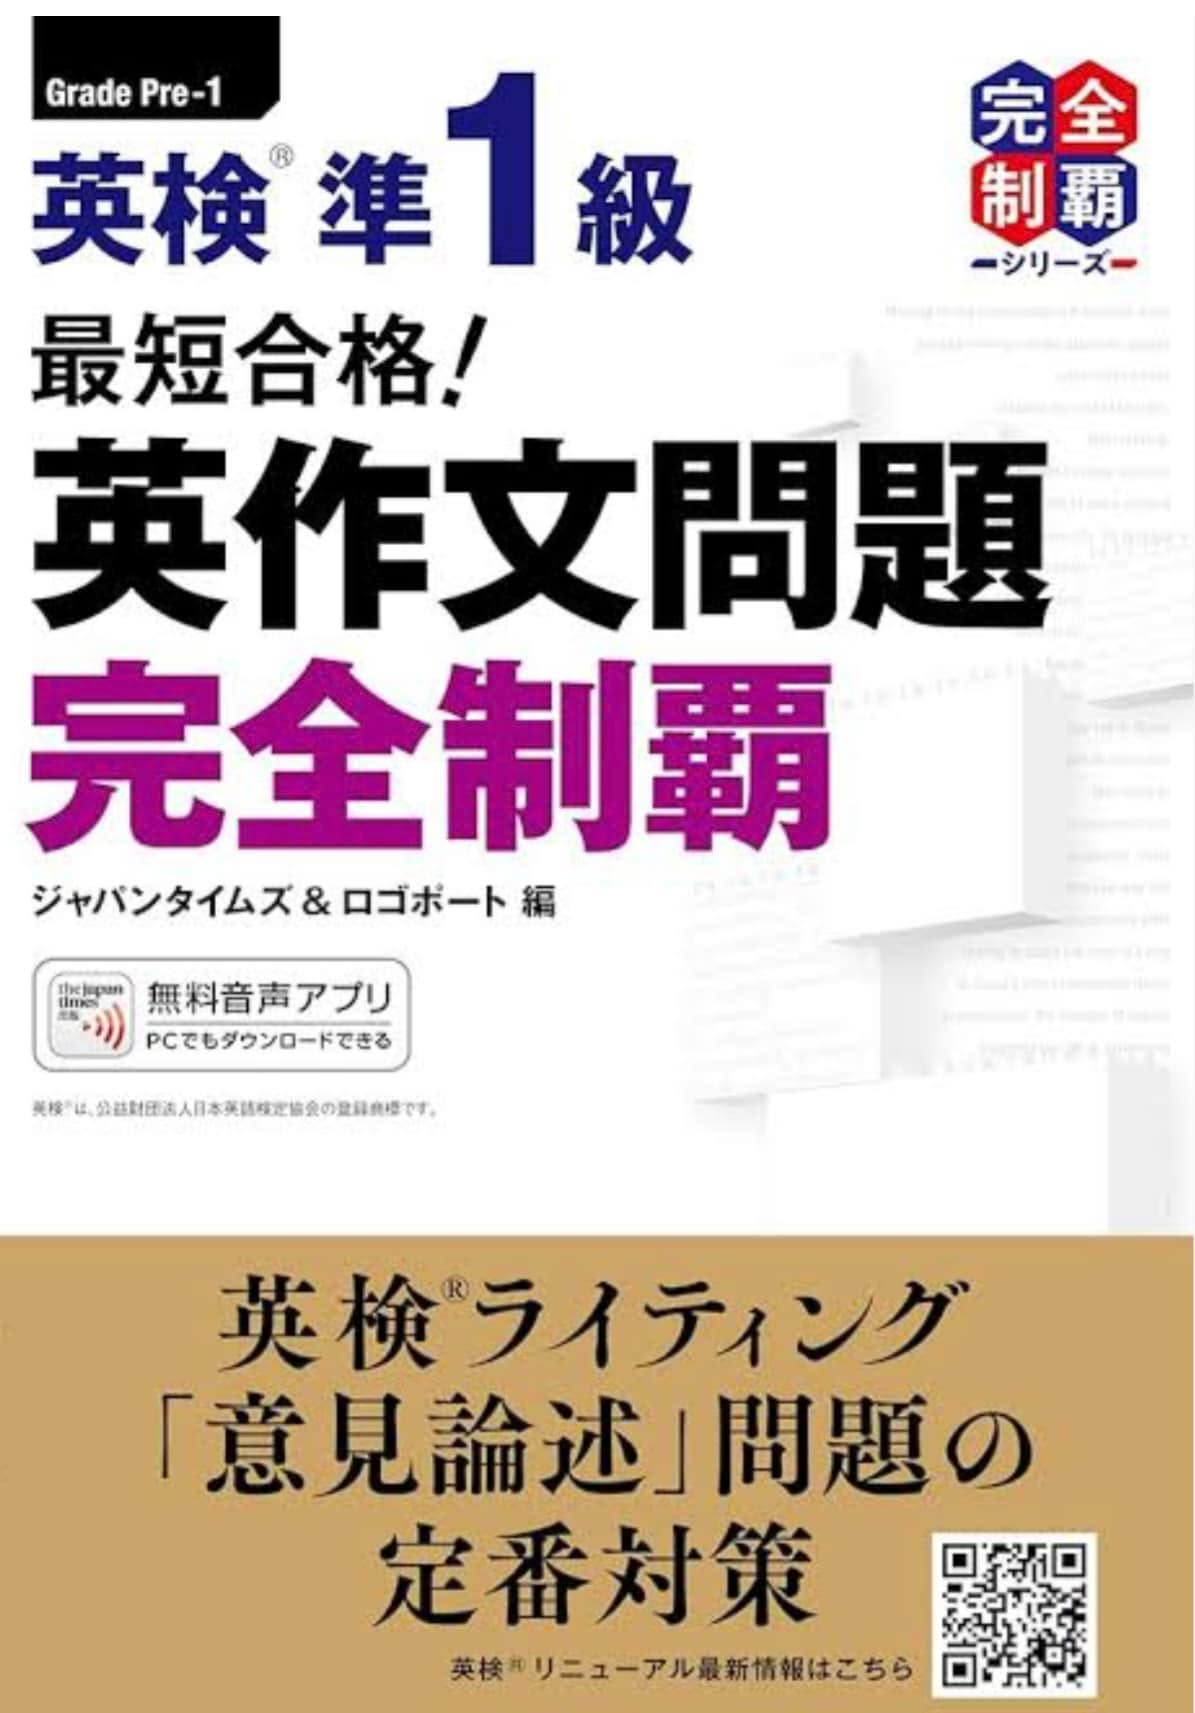
\includegraphics[width=\linewidth]{pictures/2024/07/20240709_144005_002.jpg}
\end{minipage}
\end{center}

\begin{center}
\begin{minipage}{0.48\linewidth}
\centering
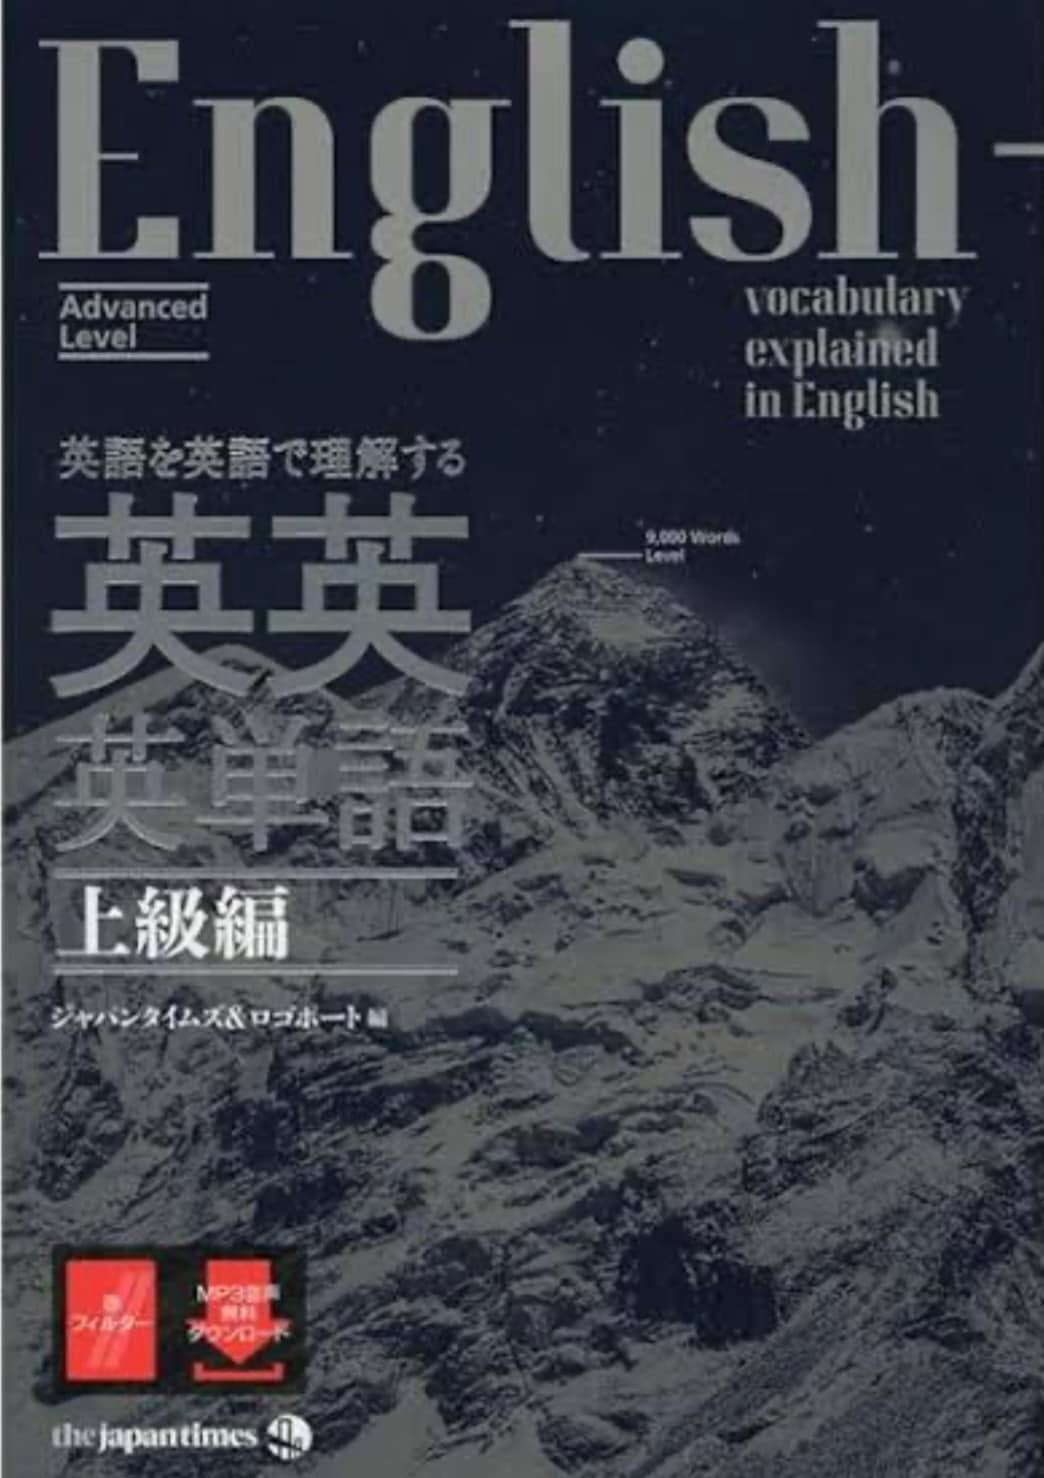
\includegraphics[width=\linewidth]{pictures/2024/07/20240709_144005_003.jpg}
\end{minipage}
\hfill
\begin{minipage}{0.48\linewidth}
\centering
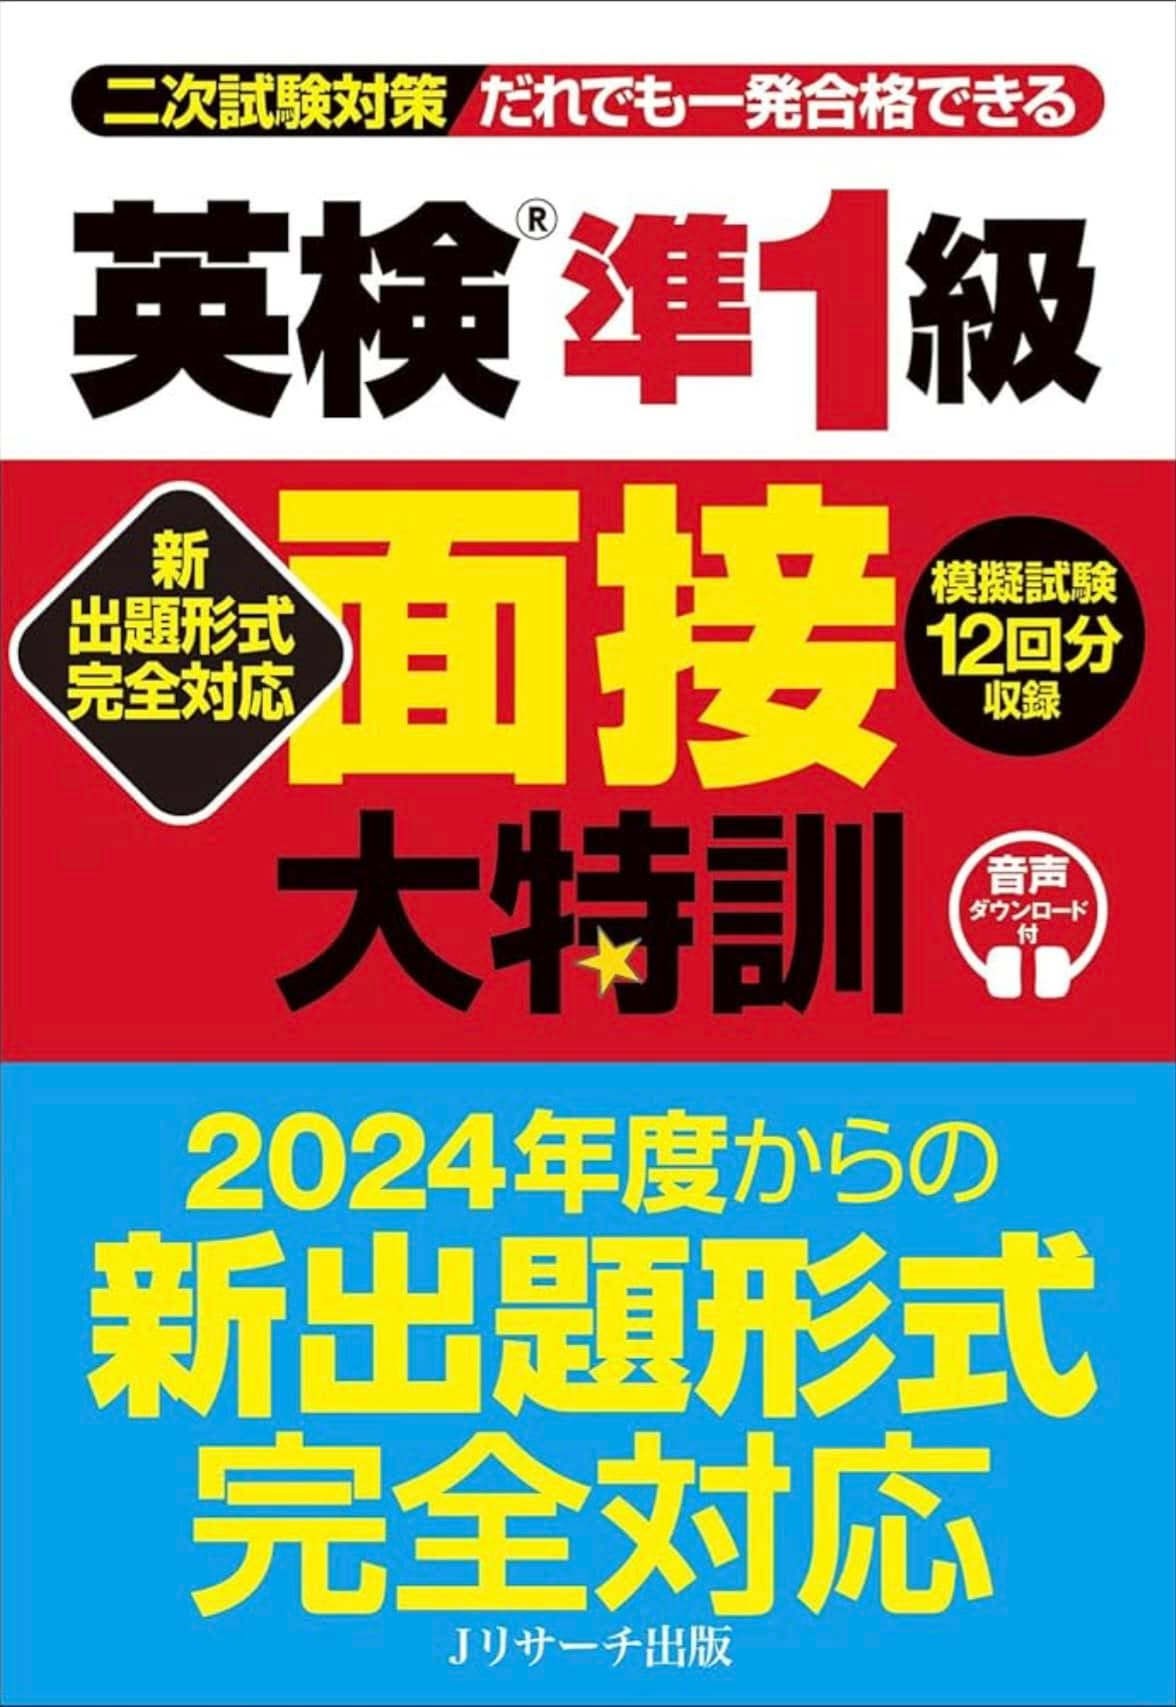
\includegraphics[width=\linewidth]{pictures/2024/07/20240709_144005_004.jpg}
\end{minipage}
\end{center}

\subsection*{2024年07月17日 01:23}
\addcontentsline{toc}{subsection}{2024年07月17日 01:23}

\url{https://youtu.be/xljWbyxOaH8}

\begin{center}
\href{https://youtu.be/xljWbyxOaH8}{
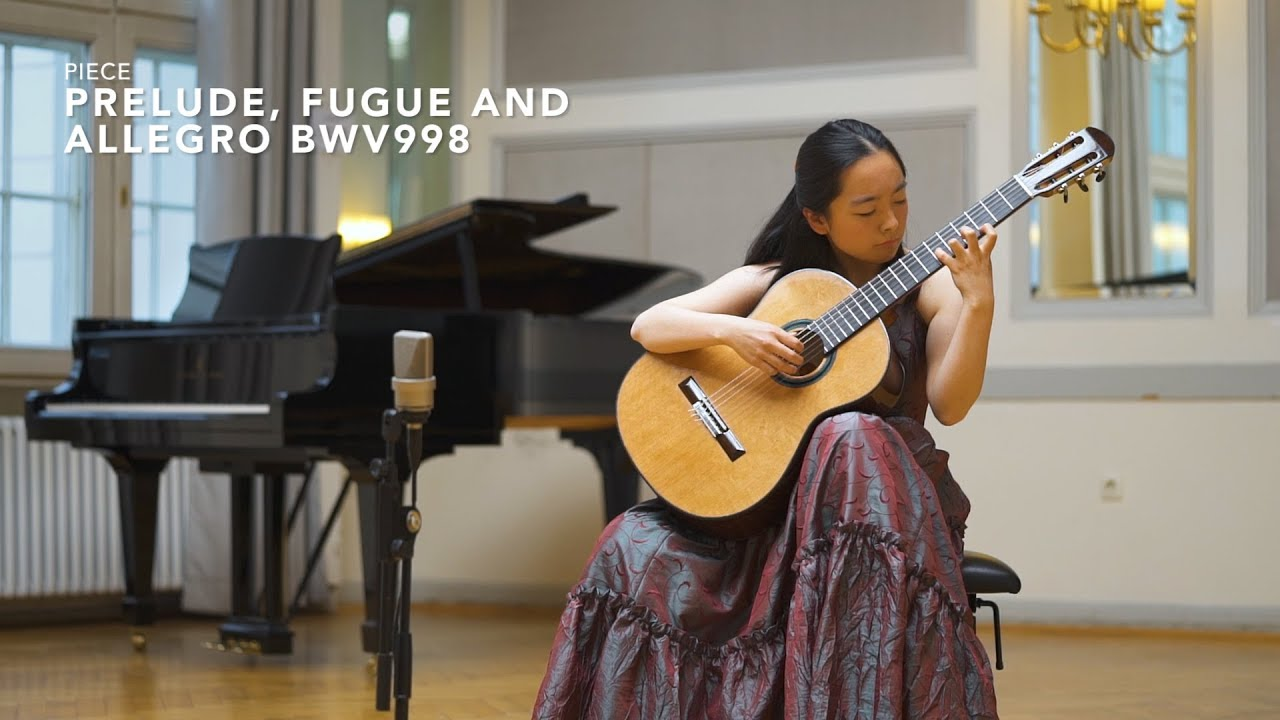
\includegraphics[width=0.48\linewidth]{pictures/youtube/2024/07/20240717_012321_youtube_001_xljWbyxOaH8.jpg}
}
\end{center}




大好きな曲です（この曲、人気ですね。自分でも弾けたらいいなあ）


J.S.Bachのライプツィヒ時代の作品。自筆譜が残されており、日本の上野学園大学が所蔵していた（最近閉校になっている。楽譜の行方は？）自筆譜には「リュート或いはチェンバロのための」という記述があるらしい。


お父上は演奏スキル世界一のあの方ですね、きっと。あの当時は確か、演奏旅行しながら同時に長崎大学の学生でいらっしゃいました。\#展覧会の絵 のギター編曲や、その演奏（not CD but）レコードのリリースがあった時には天才かと大騒ぎでした。演奏会に伺ったこともありました。サークルのメンバーで楽屋まで押しかけ、直接お話しを聞かせてもらったことも覚えています。


お父上譲りの確かな演奏技術をお持ちの上での \#Bach です。フレージング等がわざとらしくなく、しかししっかりと、自然な流れの中に（ごまかしなく）表現されている様な気がします。テンポ・ルバートがとても良い（あんばい）です。\#Prelude だけでなく \#Fugue、\#Allegro も続けて聞きたかったな。


\#山下愛陽 \#山下和仁 \#クラシックギター \#classicalguitar \#BWV998

\subsection*{2024年07月18日 16:58}
\addcontentsline{toc}{subsection}{2024年07月18日 16:58}

\paragraph{リンク}
\url{https://youtu.be/xljWbyxOaH8}

\begin{center}
\href{https://youtu.be/xljWbyxOaH8}{
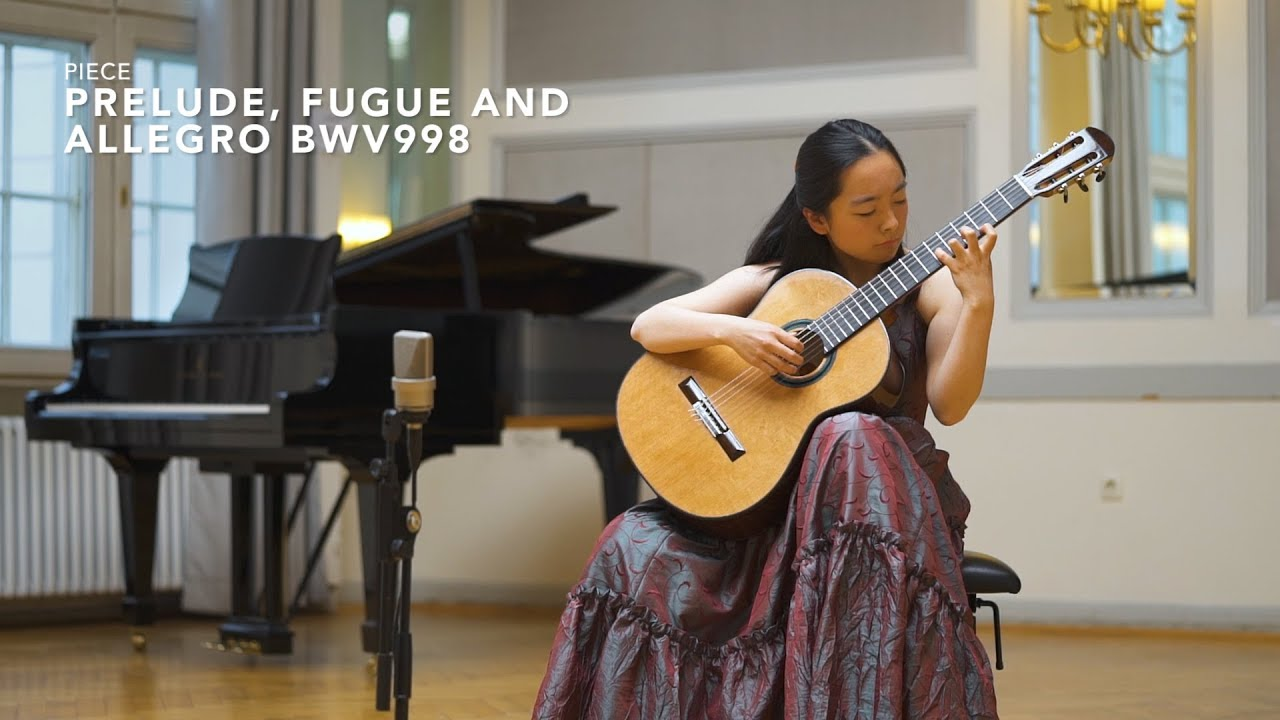
\includegraphics[width=0.48\linewidth]{pictures/youtube/2024/07/20240718_165845_youtube_001_xljWbyxOaH8.jpg}
}
\end{center}

\subsection*{2024年07月18日 21:26}
\addcontentsline{toc}{subsection}{2024年07月18日 21:26}

\paragraph{リンク}
\url{https://youtu.be/VEoOToX_PuE}

\begin{center}
\href{https://youtu.be/VEoOToX_PuE}{
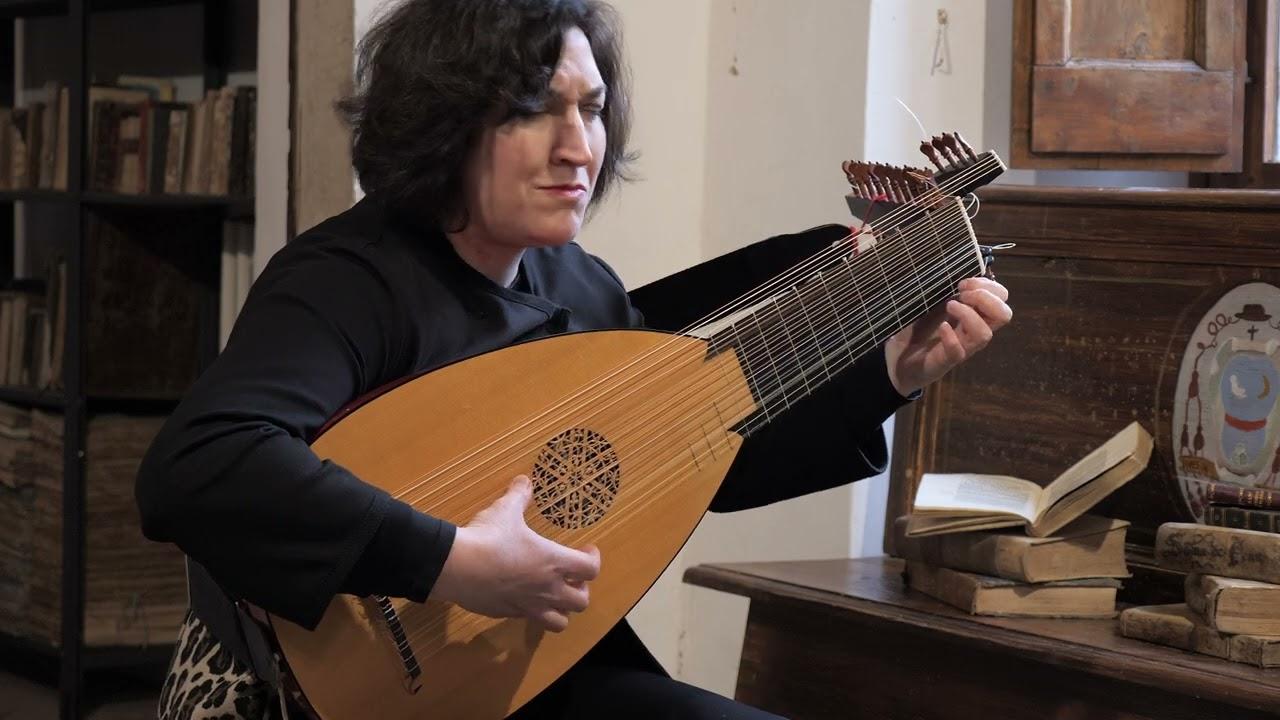
\includegraphics[width=0.48\linewidth]{pictures/youtube/2024/07/20240718_212622_youtube_001_VEoOToX_PuE.jpg}
}
\end{center}

\subsection*{2024年07月19日 13:13}
\addcontentsline{toc}{subsection}{2024年07月19日 13:13}

気になる

\paragraph{リンク}
\url{https://x.com/l_d_landau/status/1813889734378500266?s=12&t=5VtsOkpki6juEjPXsBq8hg}

\subsection*{2024年07月19日 15:37}
\addcontentsline{toc}{subsection}{2024年07月19日 15:37}

\paragraph{リンク}
\url{https://gendai.media/articles/-/133027}

\subsection*{2024年07月20日 21:02}
\addcontentsline{toc}{subsection}{2024年07月20日 21:02}

\url{https://youtu.be/rgTMg79b2qo}

\begin{center}
\href{https://youtu.be/rgTMg79b2qo}{
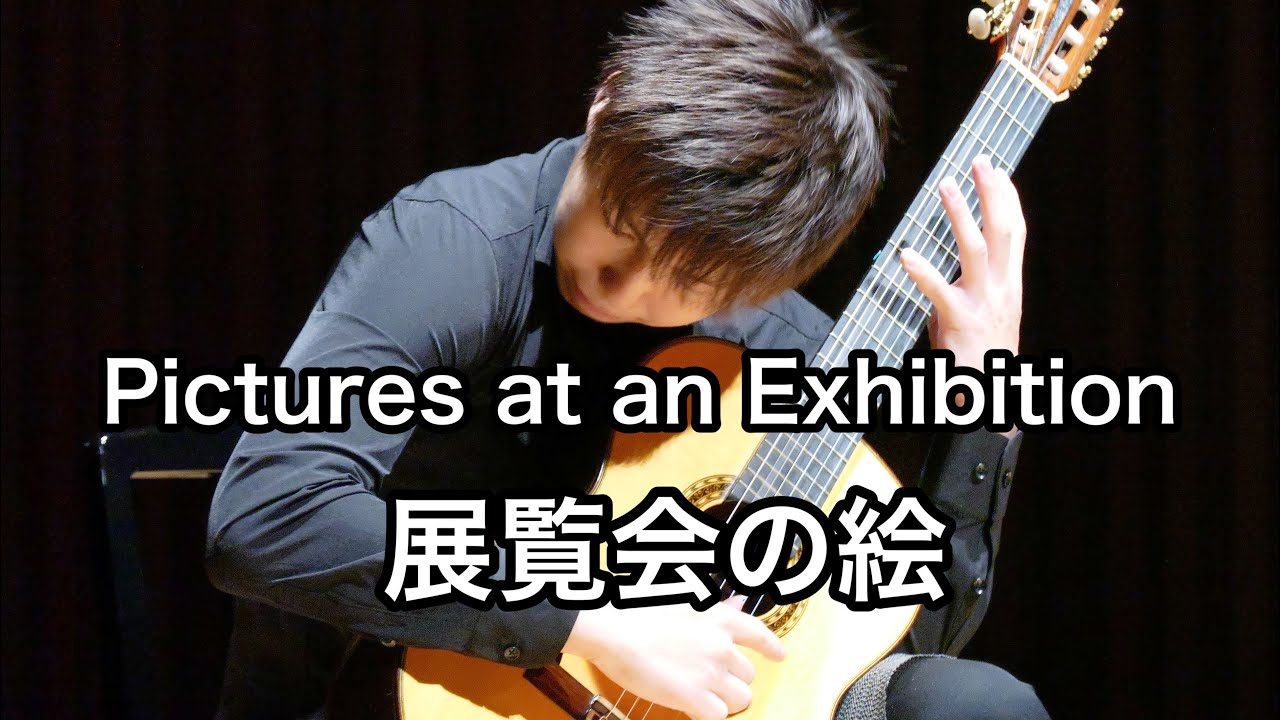
\includegraphics[width=0.48\linewidth]{pictures/youtube/2024/07/20240720_210242_youtube_001_rgTMg79b2qo.jpg}
}
\end{center}




\#編曲 者の \#山下和仁 氏以外で、これをこんなにも弾けた人がいたのか。


オーケストラの魔術師と呼ばれているラヴェルによるこの曲のオケ編も、もちろんたくさんの音色をオケで聞かせてくれるのですけれども、ギターって、ギター一本でこれ程にもたくさんの音色、音を表現出来るものなのですね。ギターの可能性を何十倍にも拡大した（編曲と）演奏ですね。


とにかく凄いってことに尽きる。

山下和仁氏が編曲して演奏したのも、ここで演奏している原田さんと同じ位の年齢だったんですね。編曲も演奏も若者であればこその挑戦なのかもしれない。


\#classicalguitar \#クラシックギター \#展覧会の絵

\subsection*{2024年07月20日 21:14}
\addcontentsline{toc}{subsection}{2024年07月20日 21:14}

\paragraph{リンク}
\url{https://youtu.be/DjOQ69JjTRo}

\begin{center}
\href{https://youtu.be/DjOQ69JjTRo}{
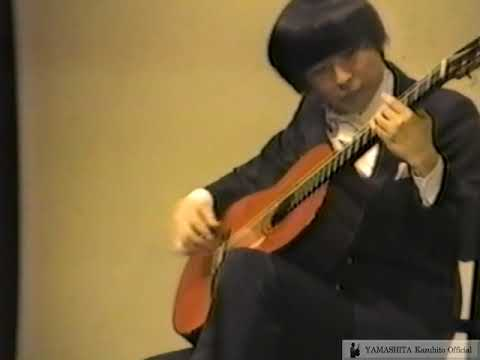
\includegraphics[width=0.48\linewidth]{pictures/youtube/2024/07/20240720_211420_youtube_001_DjOQ69JjTRo.jpg}
}
\end{center}

\subsection*{2024年07月20日 22:21}
\addcontentsline{toc}{subsection}{2024年07月20日 22:21}

⚫︎ \#RaspberryPiZero に臭気センサADRSZOD（\#TP401A）をかぶせ(\#I2C)て5分間隔で測定

⚫︎1日分の測定データは夜中にまとめて \#Googleクラウド（ストレージ）にアップロード

⚫︎別のPCではクラウドに蓄積したデータを読み込んでグラフを作図

⚫︎処理は \#shell と \#Python の組み合わせで実現

⚫︎ソースプログラム等処理の詳細（個人的備忘録）は以下に


\url{https://github.com/smat1957/RemoteSensorProject/blob/main/out/RemoteSensor.pdf}



\paragraph{写真}
\begin{center}
\begin{minipage}{0.48\linewidth}
\centering
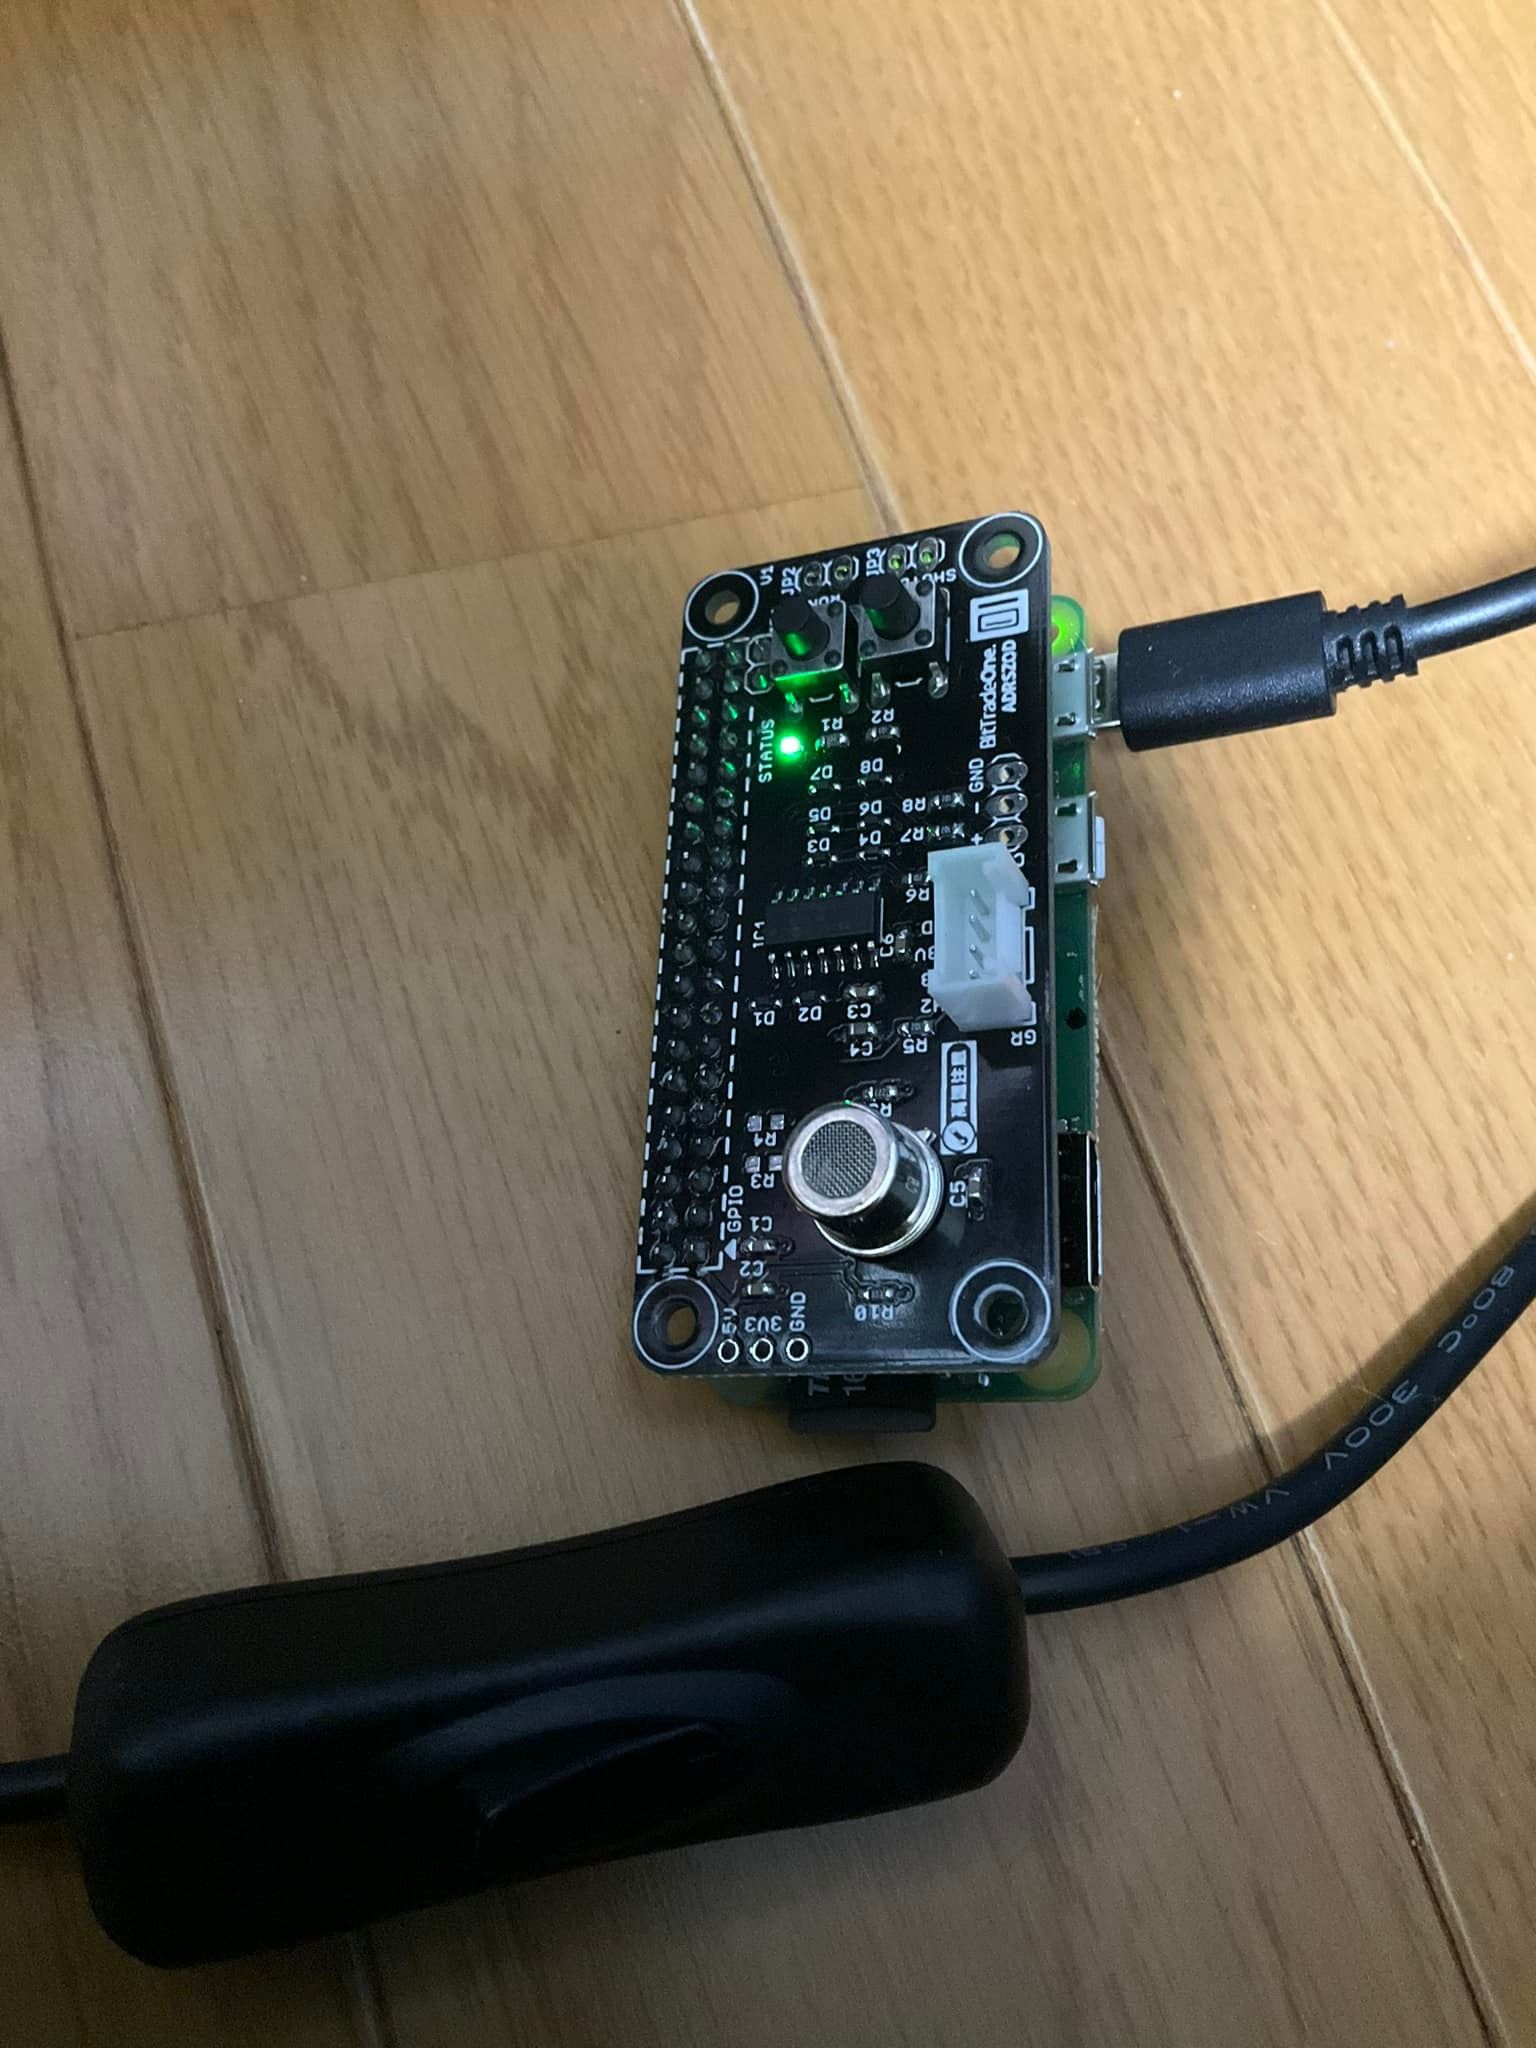
\includegraphics[width=\linewidth]{pictures/2024/07/20240720_222114_001.jpg}
\end{minipage}
\hfill
\begin{minipage}{0.48\linewidth}
\centering
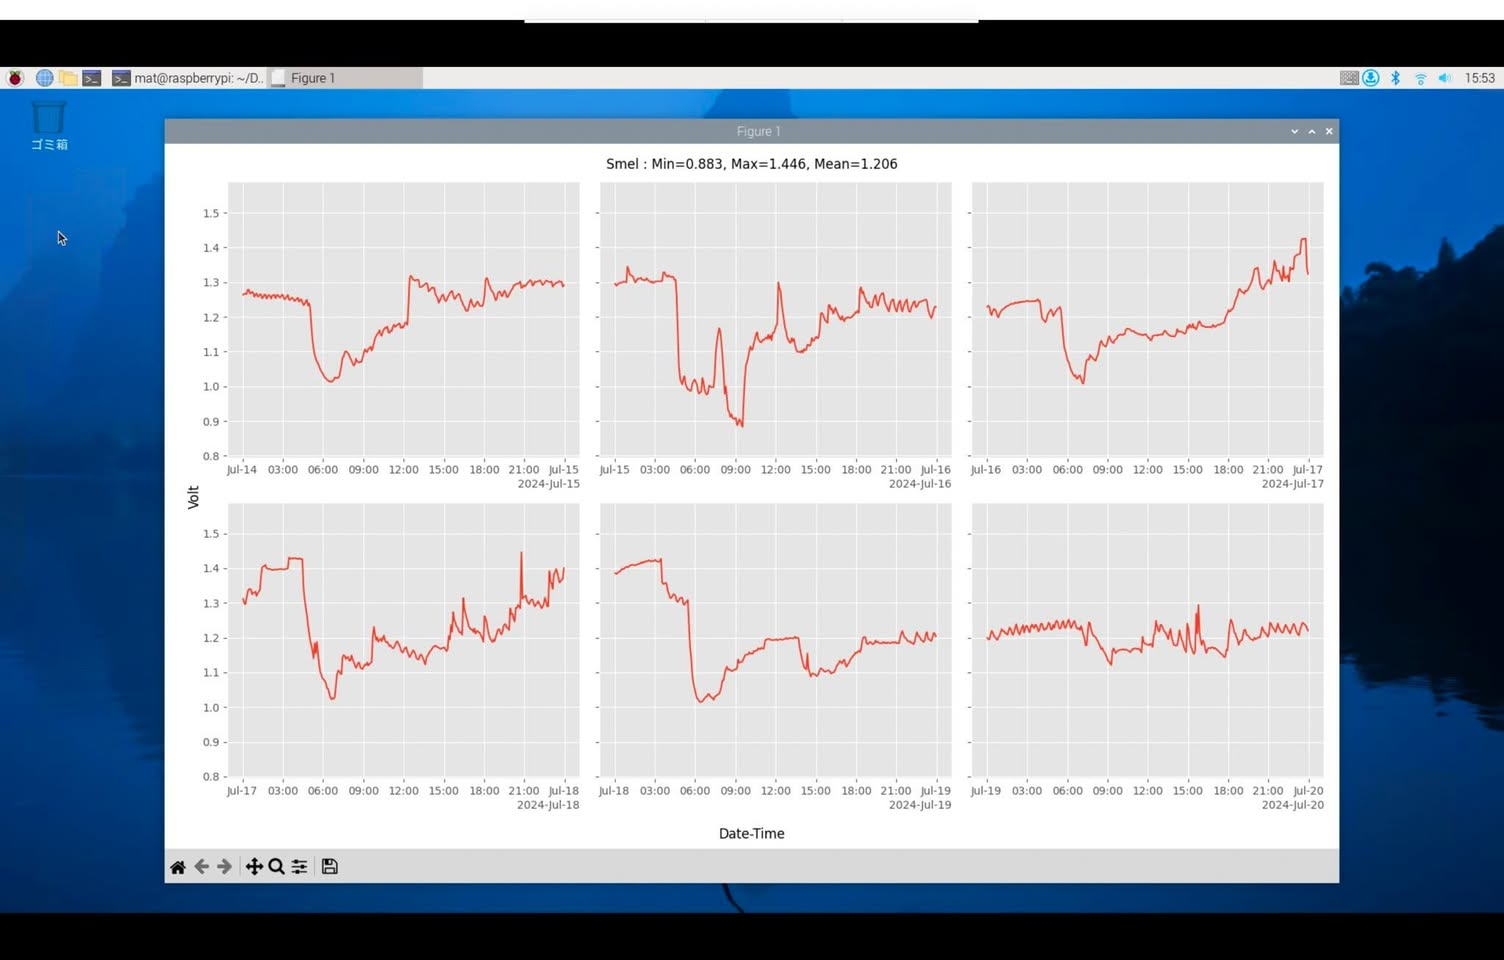
\includegraphics[width=\linewidth]{pictures/2024/07/20240720_222114_002.jpg}
\end{minipage}
\end{center}

\subsection*{2024年07月23日 04:06}
\addcontentsline{toc}{subsection}{2024年07月23日 04:06}

\paragraph{リンク}
\url{https://www.gyokusen-tei.com/}

\subsection*{2024年07月26日 15:43}
\addcontentsline{toc}{subsection}{2024年07月26日 15:43}

\#金沢城 の愛で方（私の場合）


今年になって何度か金沢城を訪れている。金沢城の愛で方は他のそれとは基本的に異なるのだと思う様になった。他の城の場合は大方のところ、天守が目的になっている事が多いのではないだろうか。「〇〇城に行ってきました」とは、「〇〇城の天守に登ってきました」と同義である事が多い様な気がする。（もちろん、お城に詳しい方の場合、今では何も建ってない様な山に登って、途中「ここには \#土塁 があった」などとの蘊蓄をお持ちの方もいらっしゃることは承知している）

そこで金沢城だが、ここには \#天守 がない。「あの辺りに \#本丸 があってそこに天守があった時代があったらしい」「本丸の天守は〇X櫓と〇△櫓と〇◻︎櫓に囲まれていたらしい」「\#櫓 というのは見張り台の様なものらしい」（櫓の中の様子は \#石川門 の中に入ってみるとその雰囲気がわかるかも）「この辺りは \#三の丸 らしい」「この辺り \#二の丸 にあった建造物の一部が再建される様だ」「\#玉泉院丸 は西の丸と呼ばれていたらしい」「\#西の丸 があるんだから、\#東の丸 というのも本丸の近くにあったらしい」などなど、、、、。ああであるらしい、こうである様だ、あそこはどうもそうだったらしいといった具合で、ああだこうだと想像を巡らせなければならない。つまり落ち着かないのだ。

これがもし天守があったなら、その天守に行って登って降りて、「金沢城に行ってきました」と、一発で落ち着く筈なのだが。そうならないのが金沢城だ。そういう事だから、「あそこはどんな風だったっけ」と、想像だけでは解決がつかなくなることもあって、確認を兼ねて何度もお城に出向かなければならなくなるのだ。

基本的に金沢城は鷹の目になって、その構造などを上から俯瞰的に眺めて理解したり、建物や城壁、石垣など、その美しさを遠目で見て愛でたりしても楽しめるお城なのだと思う様になった。


添付は、\#石川門 の中から \#兼六園 方向を見ています。初めて石川門の中に入りました。

\paragraph{写真}
\begin{center}
\begin{minipage}{0.48\linewidth}
\centering
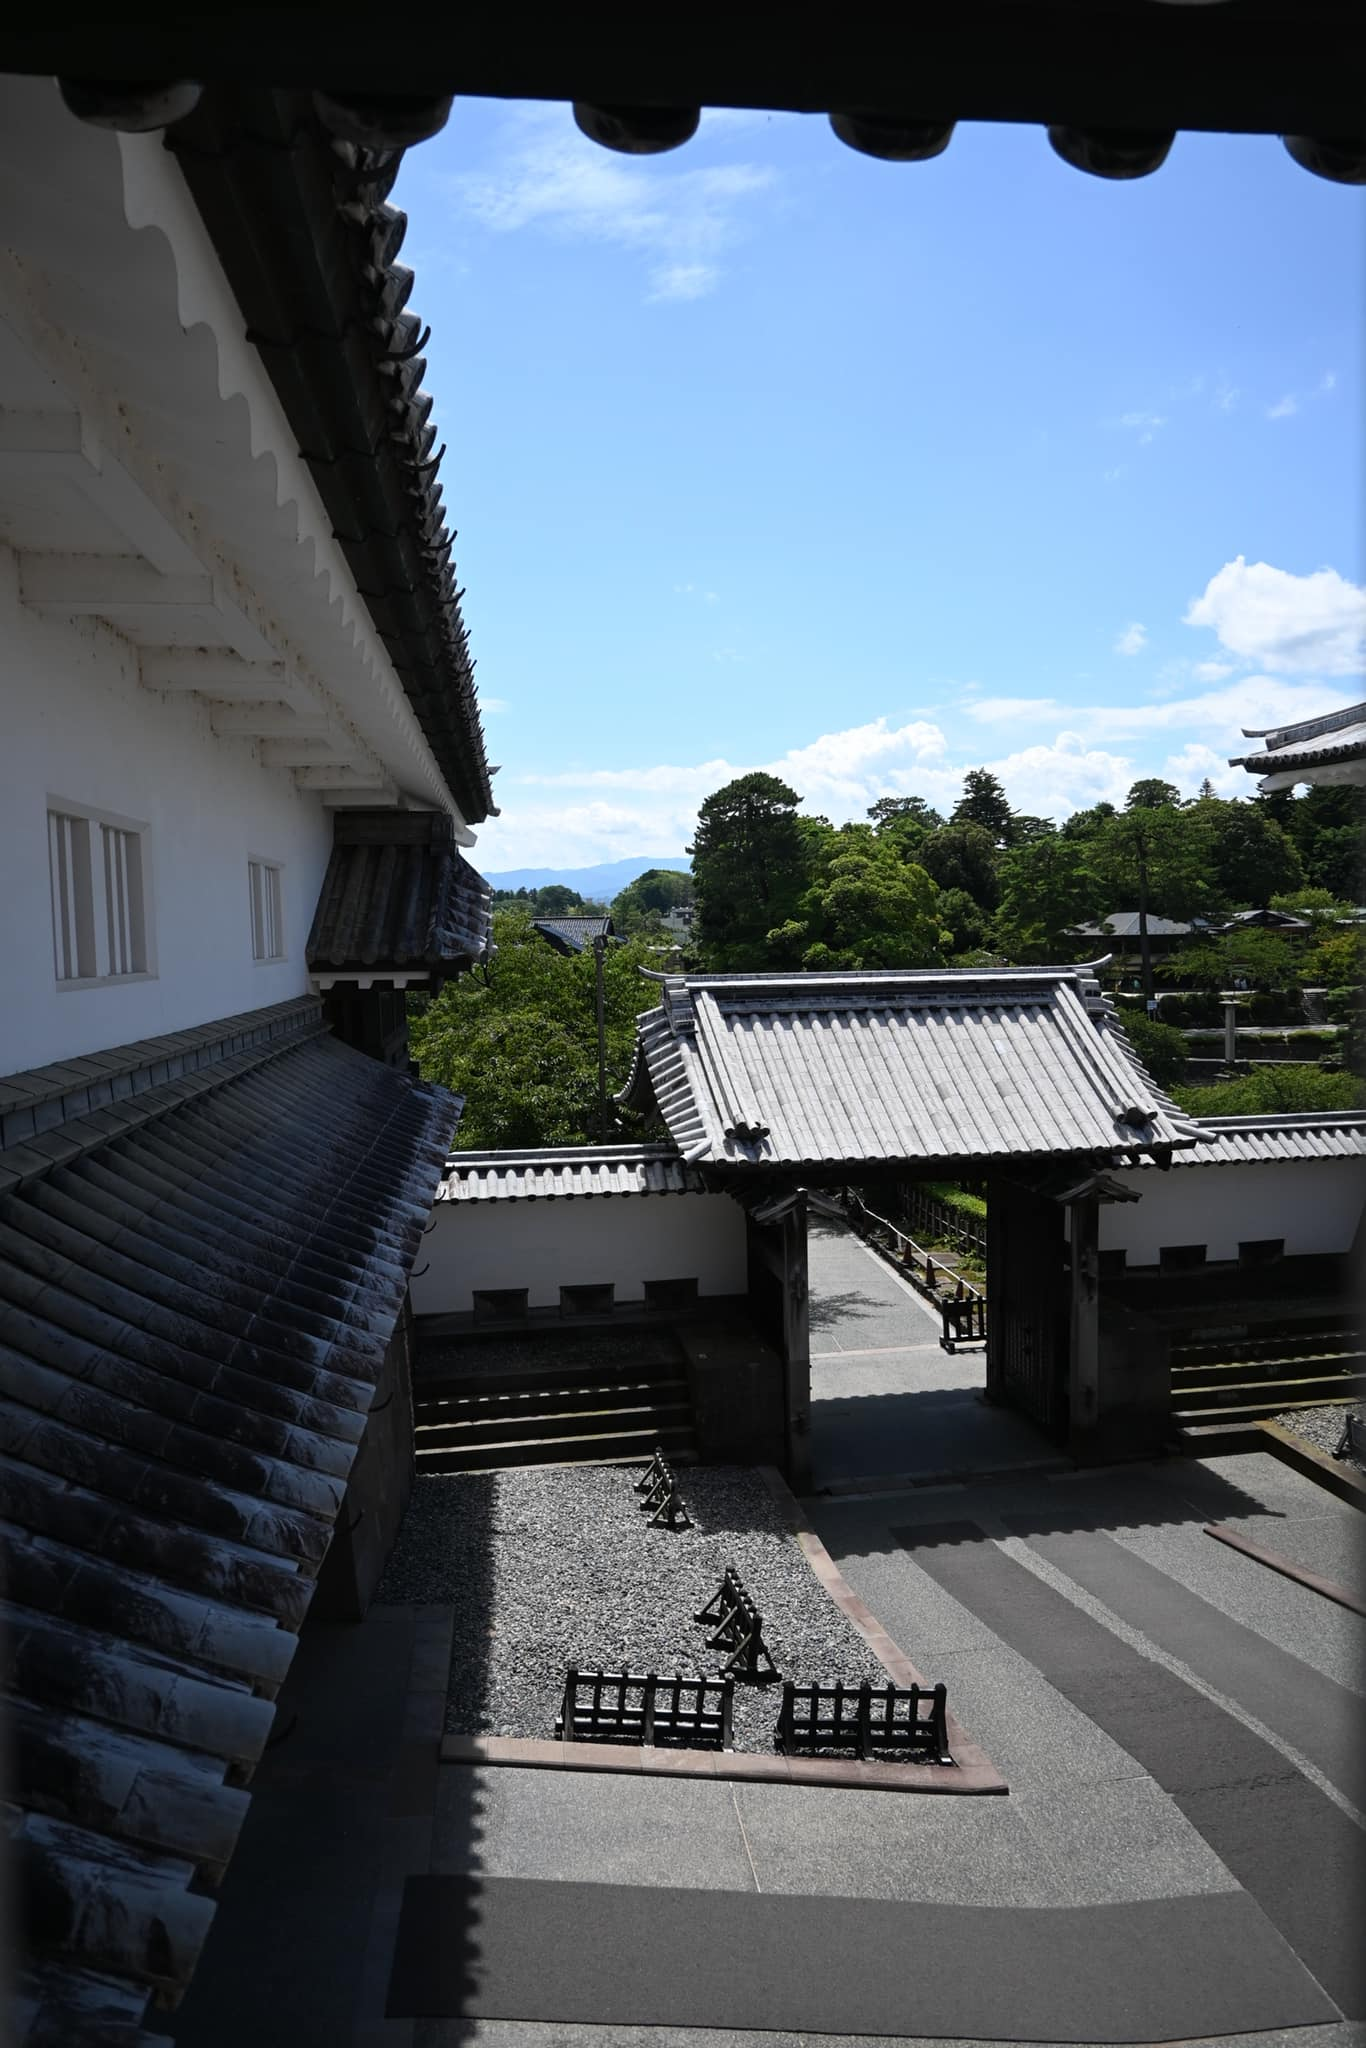
\includegraphics[width=\linewidth]{pictures/2024/07/20240726_154308_001.jpg}
\end{minipage}
\hfill
\begin{minipage}{0.48\linewidth}
\centering
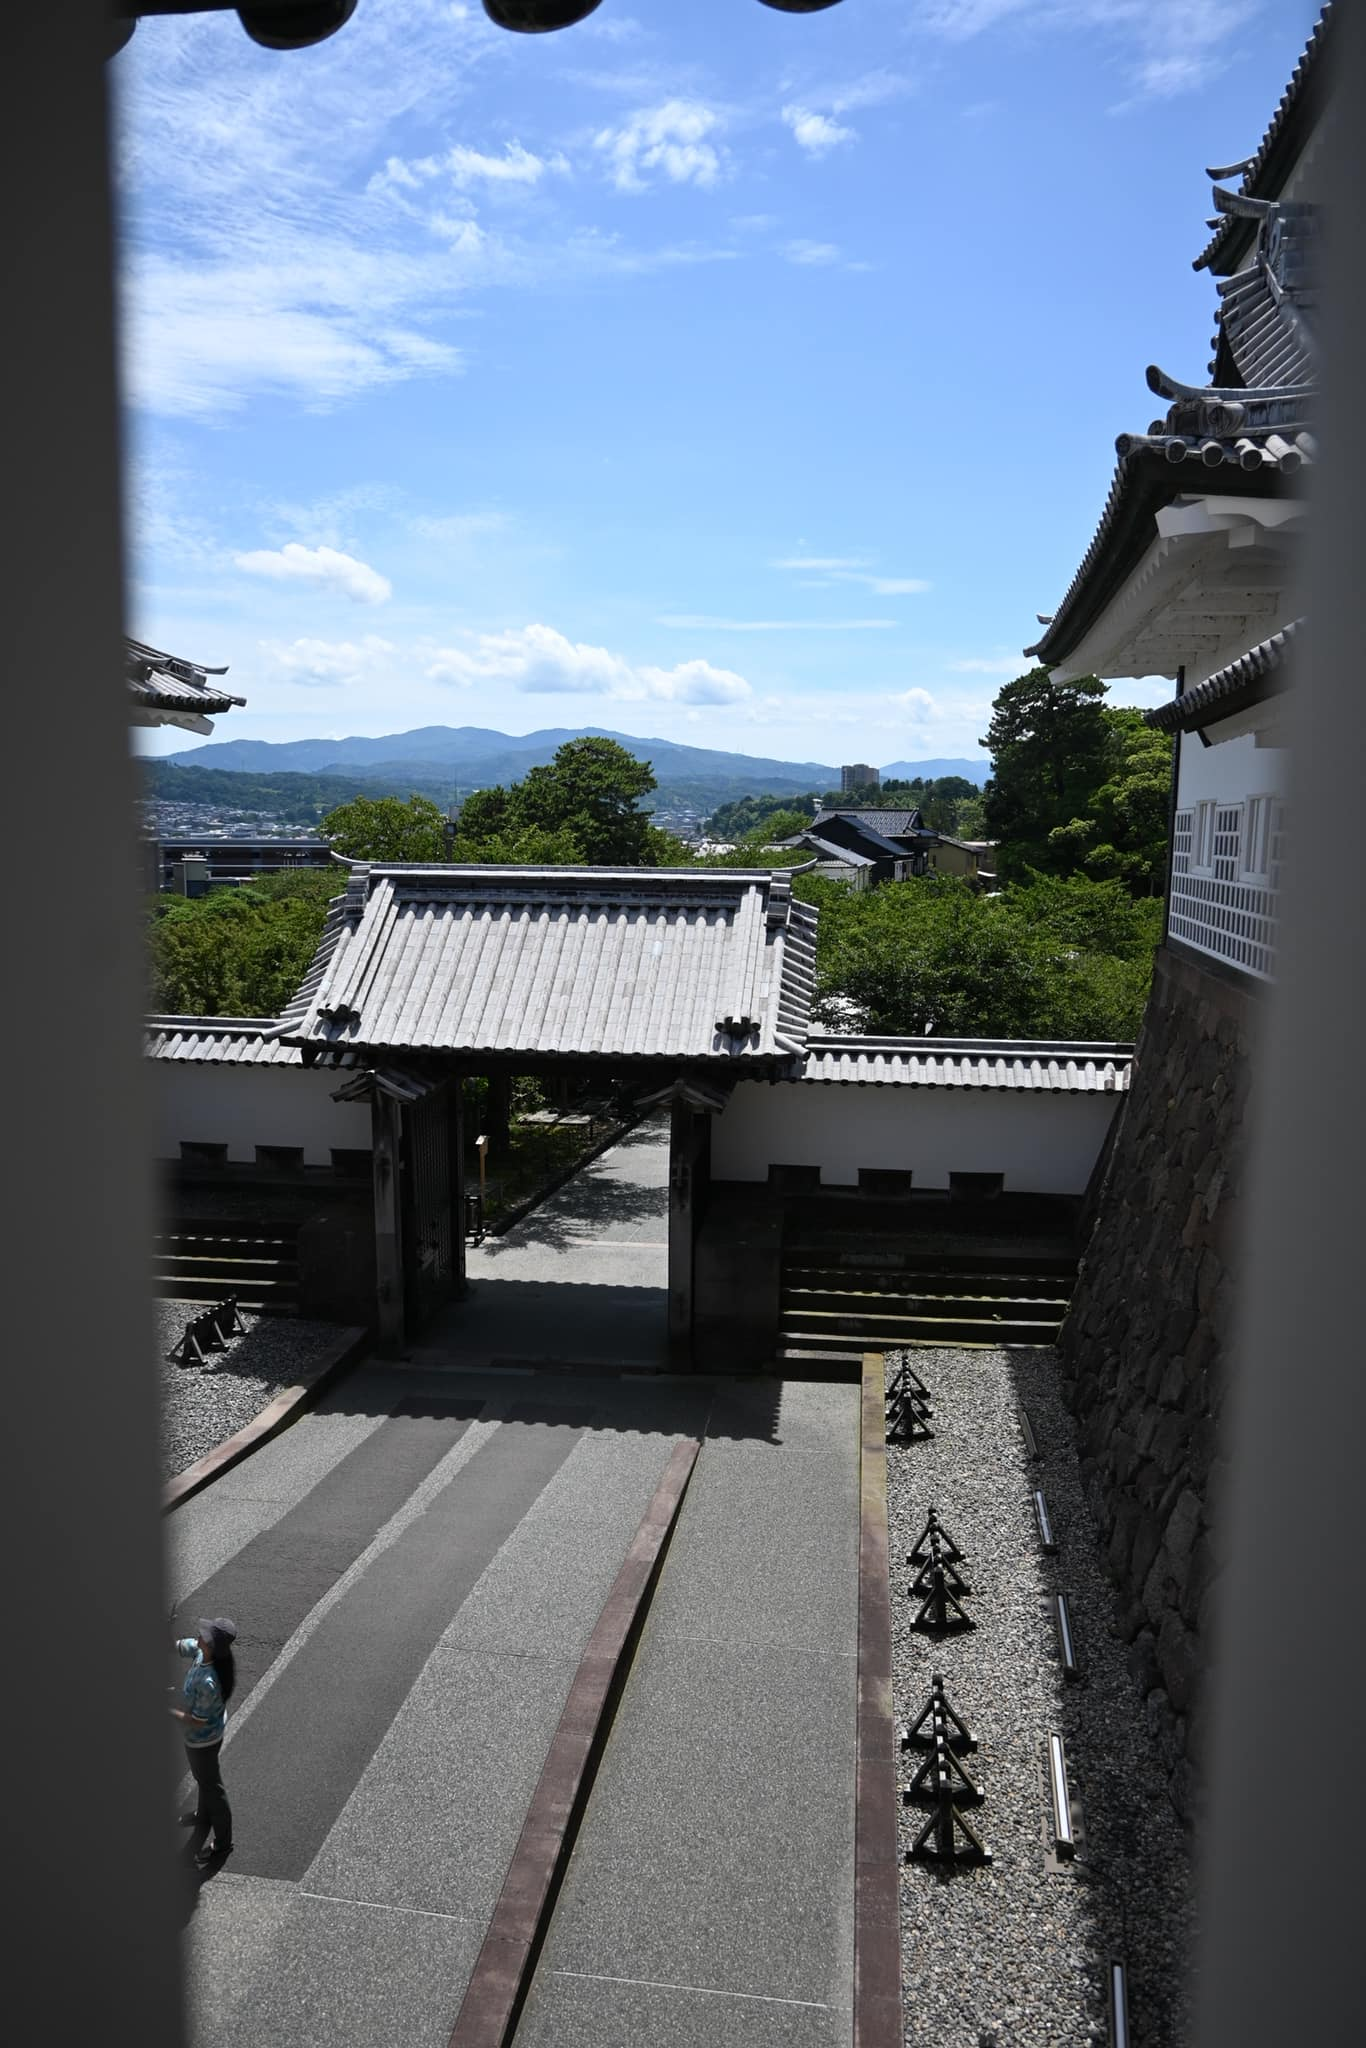
\includegraphics[width=\linewidth]{pictures/2024/07/20240726_154308_002.jpg}
\end{minipage}
\end{center}

\begin{center}
\begin{minipage}{0.48\linewidth}
\centering
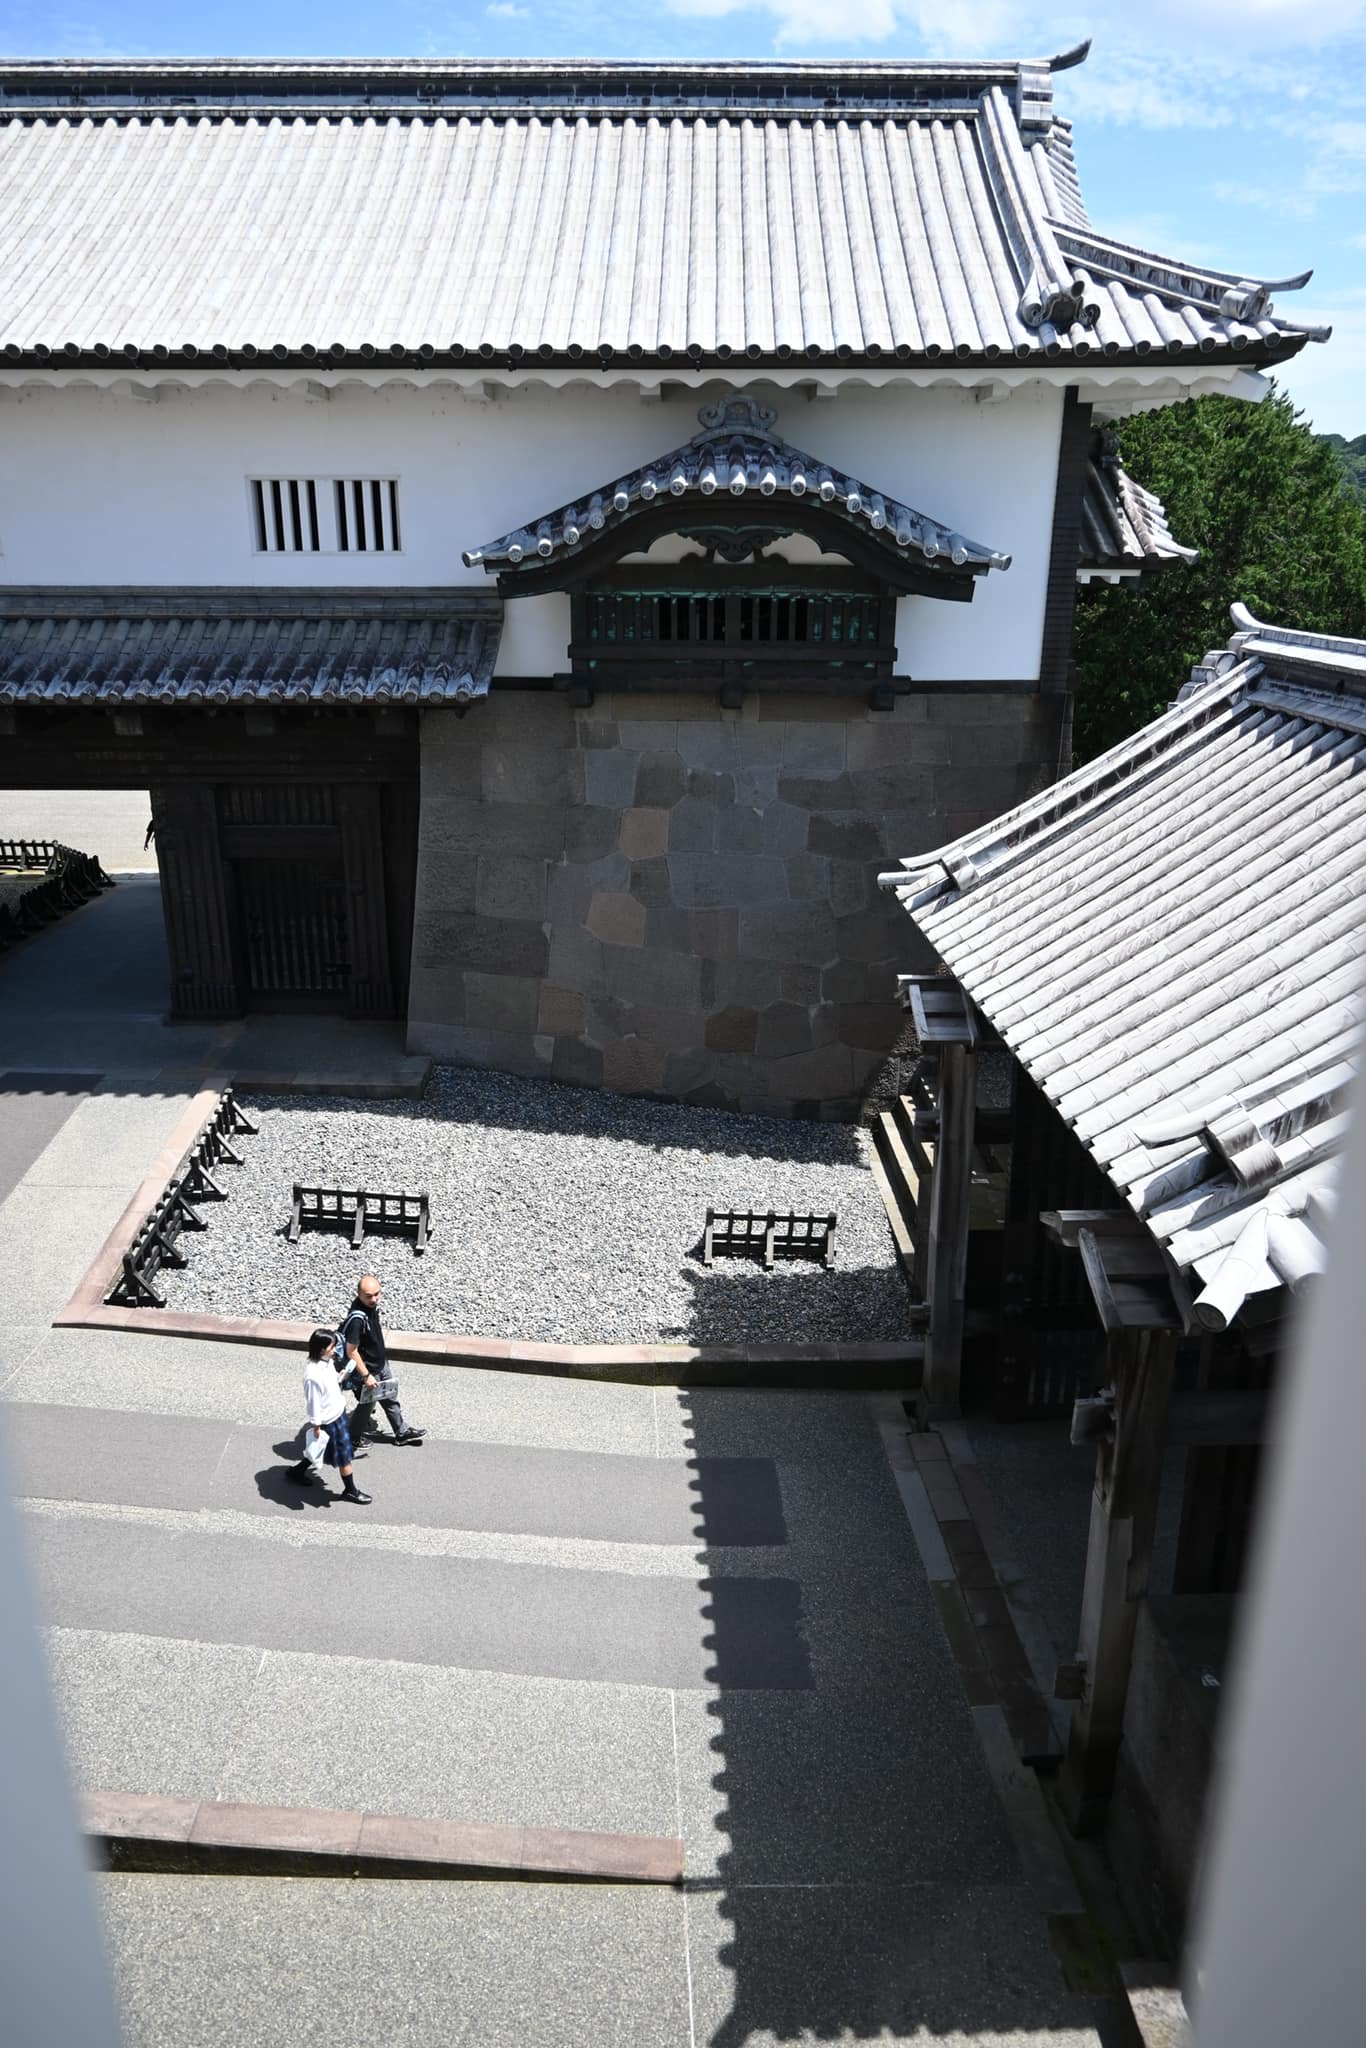
\includegraphics[width=\linewidth]{pictures/2024/07/20240726_154308_003.jpg}
\end{minipage}
\end{center}

\subsection*{2024年07月27日 03:35}
\addcontentsline{toc}{subsection}{2024年07月27日 03:35}

\#前田りり子 氏による  \#クヴァンツのフルート奏法を読む が今日から始まるので、聞いてみようかと思っている。\#zoom による \#オンライン講座 らしいのですが、自宅に居ながらにして受講できるのですからとっても便利。本当にそんな時代になったのですね。


「J.J. \#Quantz の \#フルート奏法」ですが、全部を読んでみたことはありません。しかし、\#トリルの運指 だけはこの本が頼りです。何せ、当時のトリルの趣味と言ったら、何となく音痴な音の並びでありながら、そのやや音痴な響きを楽しむ文化であったらしいのだから面白い。また、\#クヴァンツ が作った笛には一つ余分（？)な \#キー が付いている（レのシャープとミのフラットを吹き分けるという）。その運指もこの本によらなければならない。そもそも \#平均律 とそうでないものを音楽的に聞き分ける耳を、私が持っているかというと甚だ疑問なのですが。いろいろ興味深い話を聞けるのではないかと楽しみです。

\paragraph{写真}
\begin{center}
\begin{minipage}{0.48\linewidth}
\centering
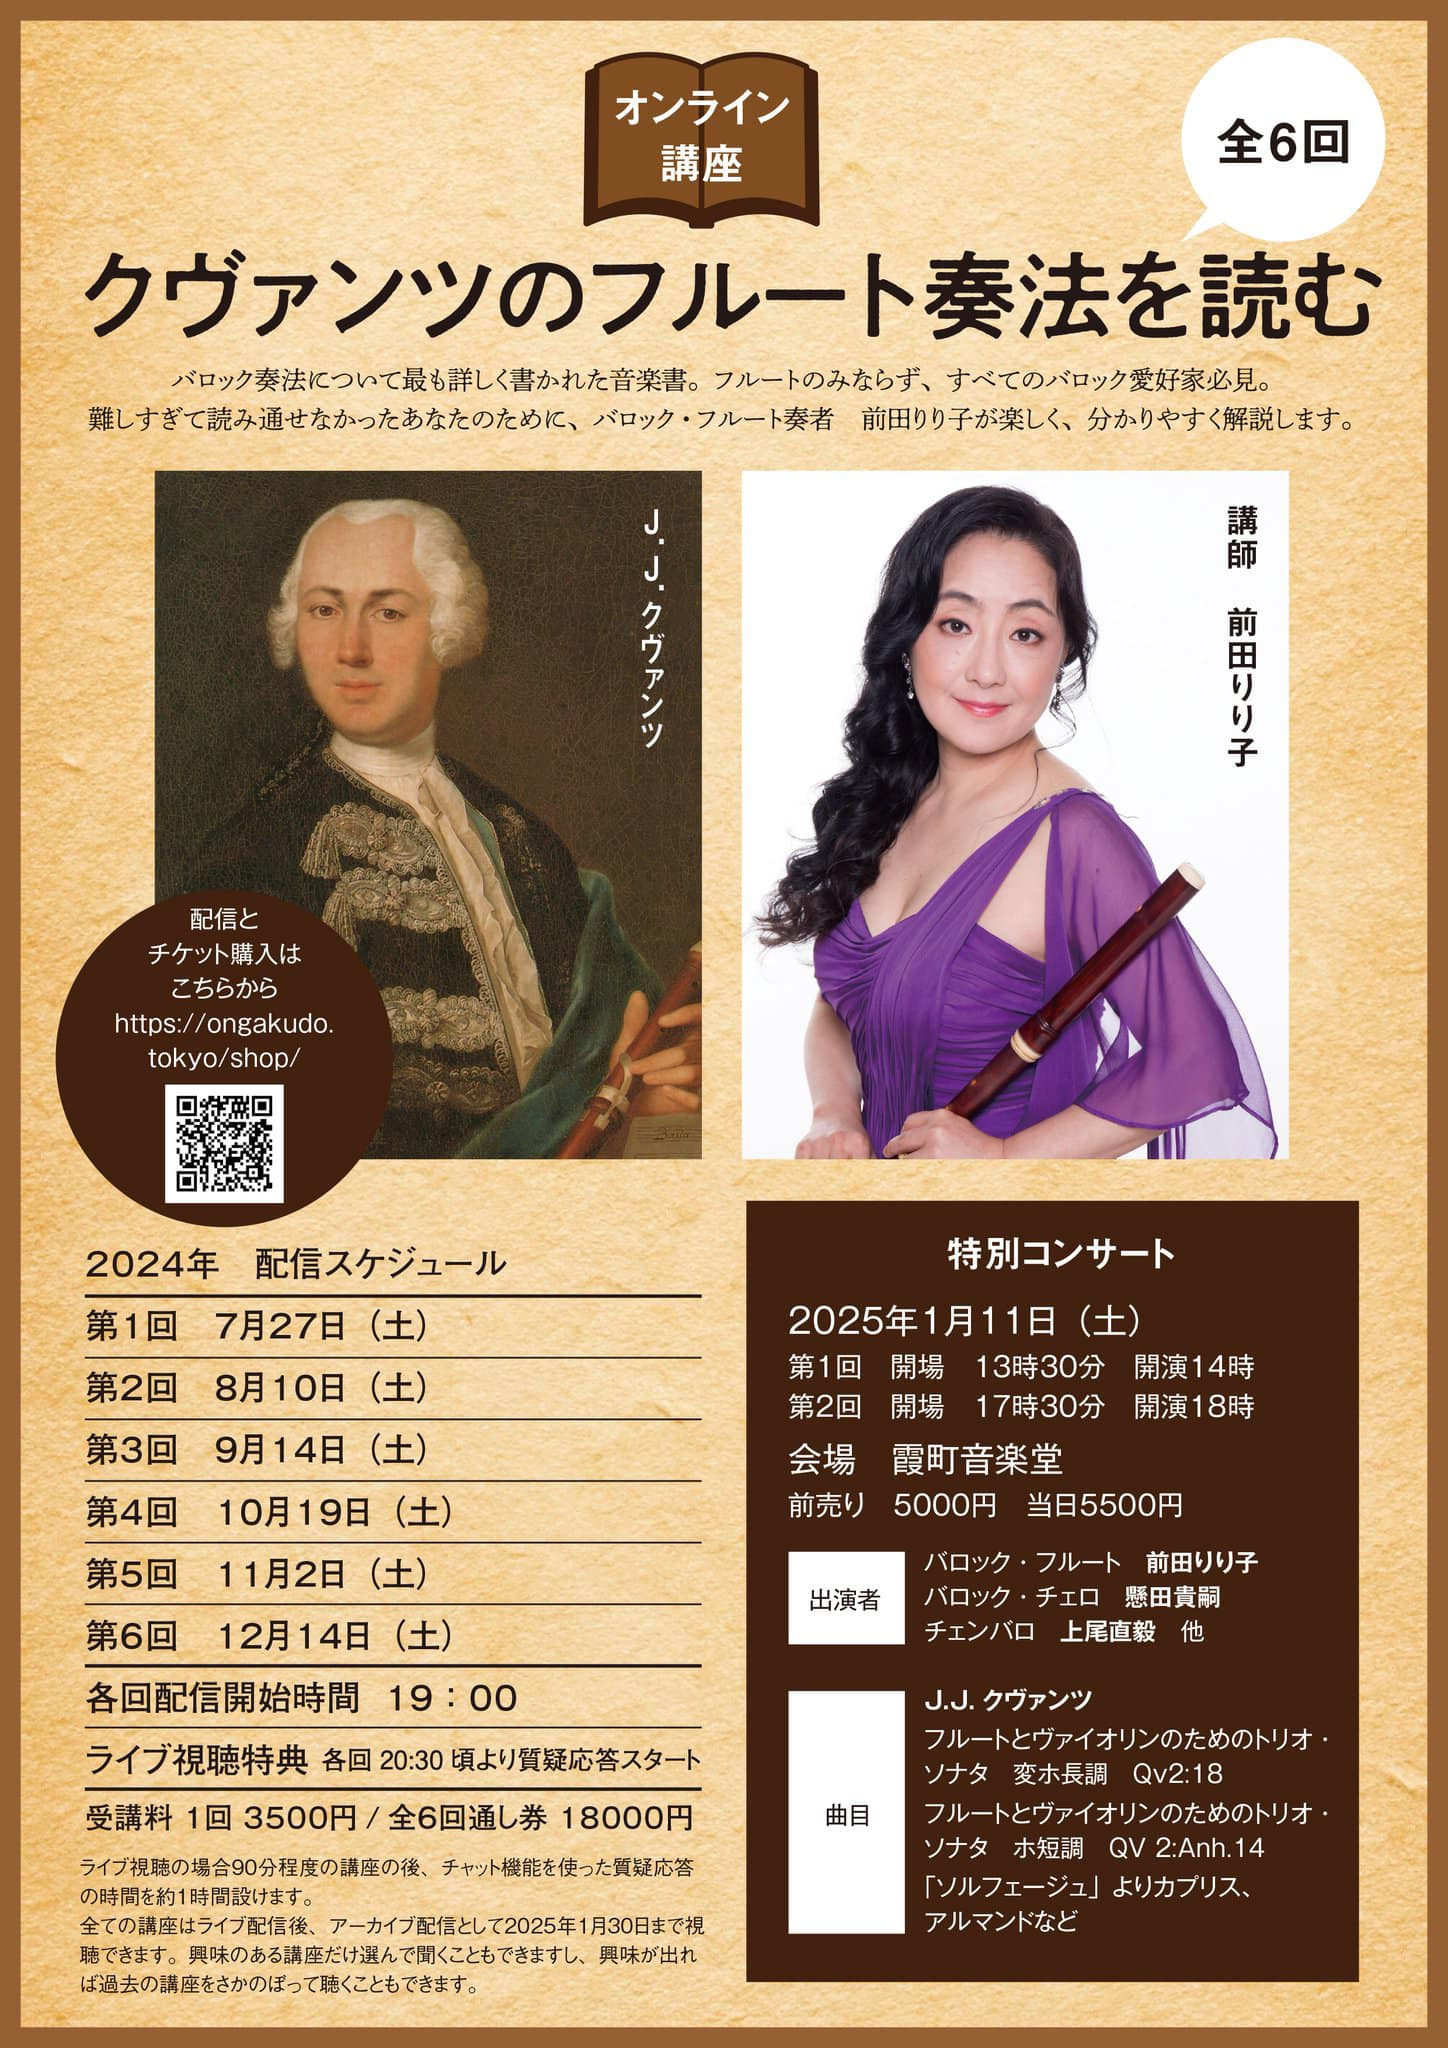
\includegraphics[width=\linewidth]{pictures/2024/07/20240727_033515_001.jpg}
\end{minipage}
\hfill
\begin{minipage}{0.48\linewidth}
\centering
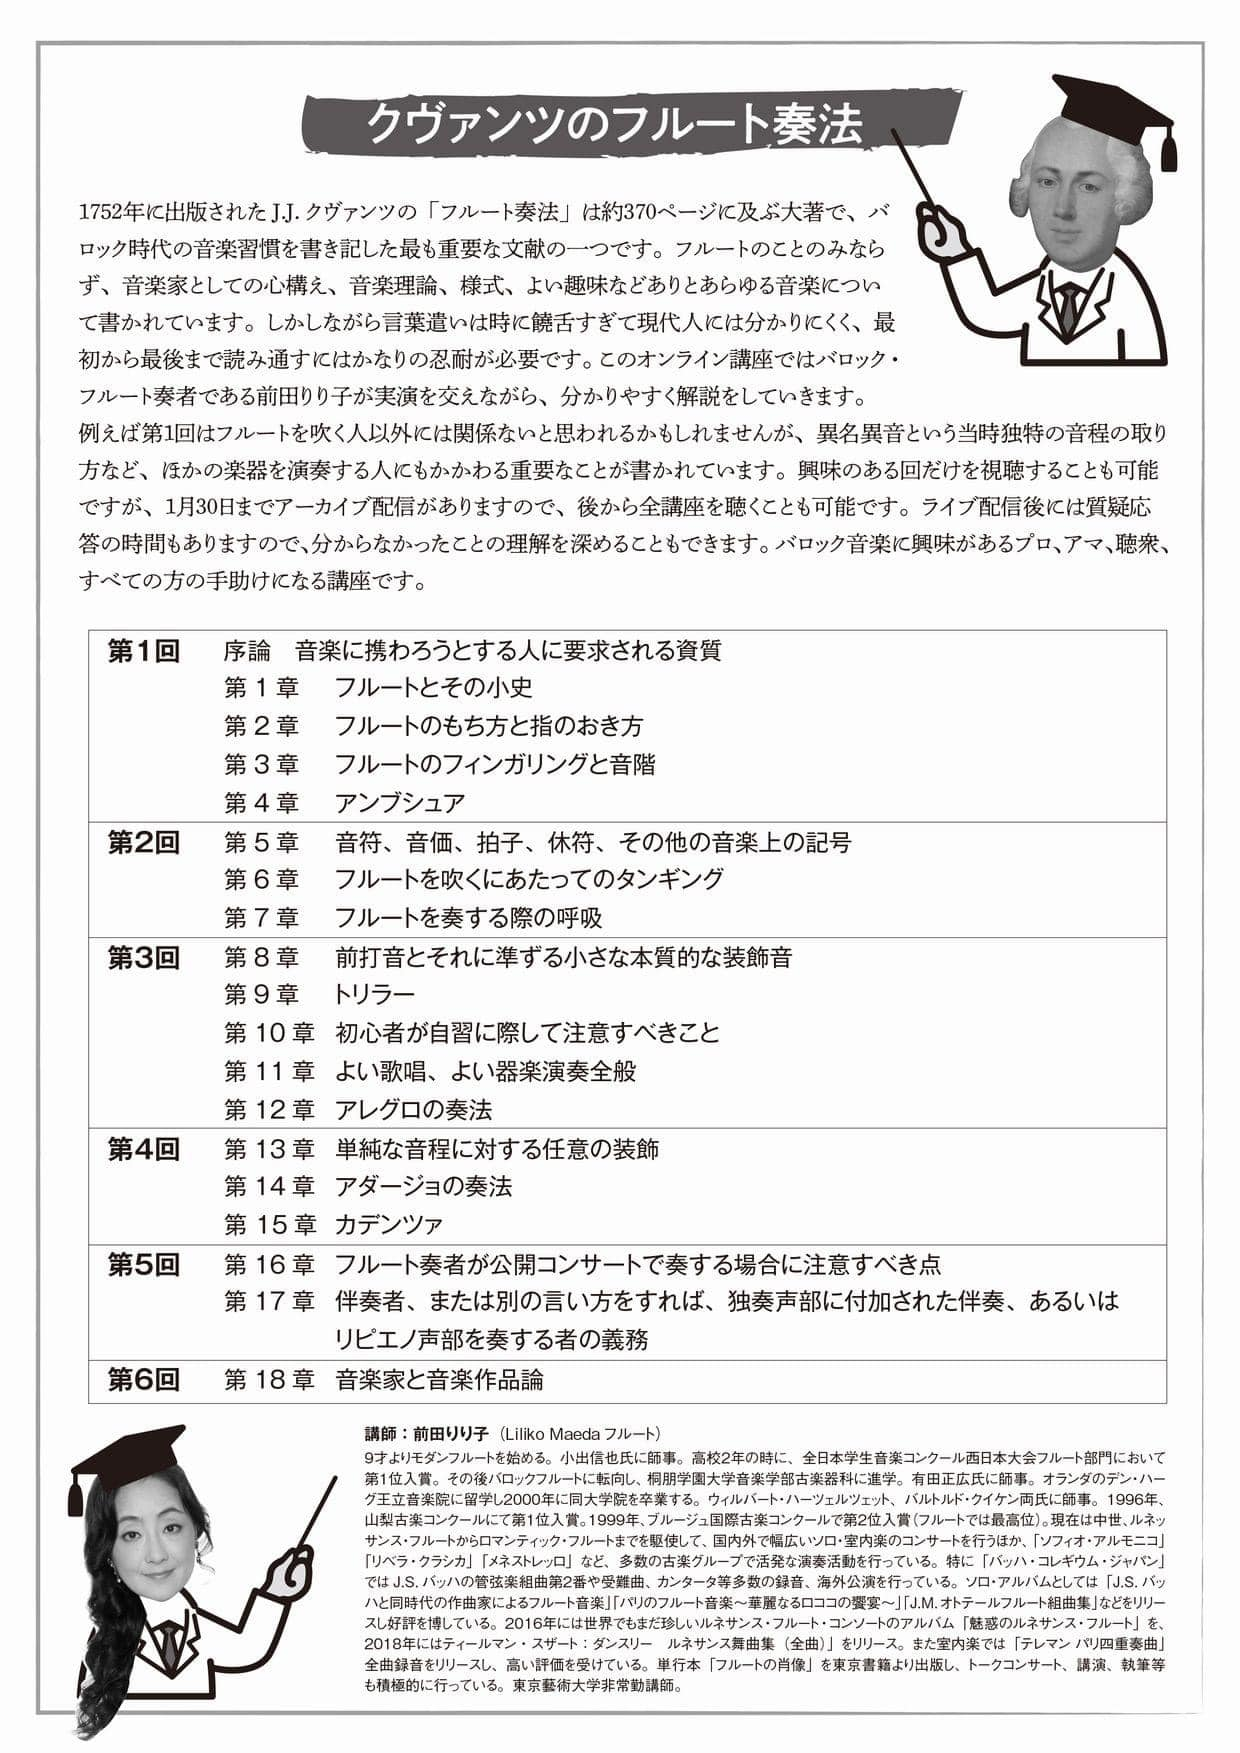
\includegraphics[width=\linewidth]{pictures/2024/07/20240727_033515_002.jpg}
\end{minipage}
\end{center}

\subsection*{2024年07月27日 23:31}
\addcontentsline{toc}{subsection}{2024年07月27日 23:31}

\url{https://www.facebook.com/photo.php?fbid=900497605450691&set=a.651711413662646&type=3}




\#フランス🇫🇷の \#オリンピック \#開会式 を見ていてつくづく感じた事があった。「自由」「平等」「博愛」が現実であるからこそ、「表現」は独創的、創造的になる事ができて、芸術の都は健在であると言う事ができるのだろうと。

マリーアントワネットの断頭台の演出然り、LGBTや人種等への偏見に対立する表現もそうだ。聖火リレーもフランス人に限っていなかったではないか。世界中のオリンピアンや表現者達が国境の隔てなく活動し、スポーツの祭典に集う喜びを表していた。何事であれ、自由に表現して発信できる環境がなければ創造的な仕事はできないのだと感じた。

雨の中、ピアノの上に落ちる雨粒が演出なんじゃないのかと思わせる様な モーリス \#ラヴェル の「\#水の戯れ」のピアノ演奏は実に素敵だった。フランスが誇る世界的な作曲家だ。演奏しているのも若者だったのが何だか嬉しかった。また、\#イマジン の静かな祈りと平和への願い、\#愛の讃歌 の熱唱など、心打たれる表現の数々だった。LEDで表現された（燃えていない）気球の \#聖火台 。派手な花火ではなく、静かにフェードアウトする開会式。そんな趣味の良さ、洗練された美しさの中にも、現代社会への様々なメッセージが込められた開会式だった。

一方、フランス🇫🇷の開会式のこれらの表現に対する日本の批判的な反応はとても残念だ。現在の日本は、様々なよく分からないものに対する忖度で身動きが取れなくなってしまっている。「断頭台の首が放送されてもいいのか」「LGBTへの偏見だと言ってしまって大丈夫か」など。表現や発信は、自由でもなければ平等でもない、もちろん友愛など考えられないほどギスギスした社会になってきている。息苦しい限りだ。「こんなこと言ったらXXに睨まれるんじゃないか」そんなことばっかり気にしていなくちゃいけないなんて。（どうって事ない年寄りの、たかだかこの程度のしょうもない記事の公開でさえ、躊躇してしまうのですから）

\subsection*{2024年07月30日 12:36}
\addcontentsline{toc}{subsection}{2024年07月30日 12:36}

学生の頃、中国から来ていた留学生に「中国ではマイクロコンピュータの事を微計算機と書くらしいね」と悪気無く（面白いねと言うニュアンスで）言ったんだけど、「日本だってCPU（Central Processing Unit）の事を中央処理装置って言うだろ」と真顔で返され、少し怯んだ事があった。


しかし、エントロピーでこの漢字を使う人はいるんだろうか？


\url{https://x.com/seimi_0501/status/1817960267126636889?s=61&t=5VtsOkpki6juEjPXsBq8hg}



\paragraph{写真}
\begin{center}
\begin{minipage}{0.48\linewidth}
\centering
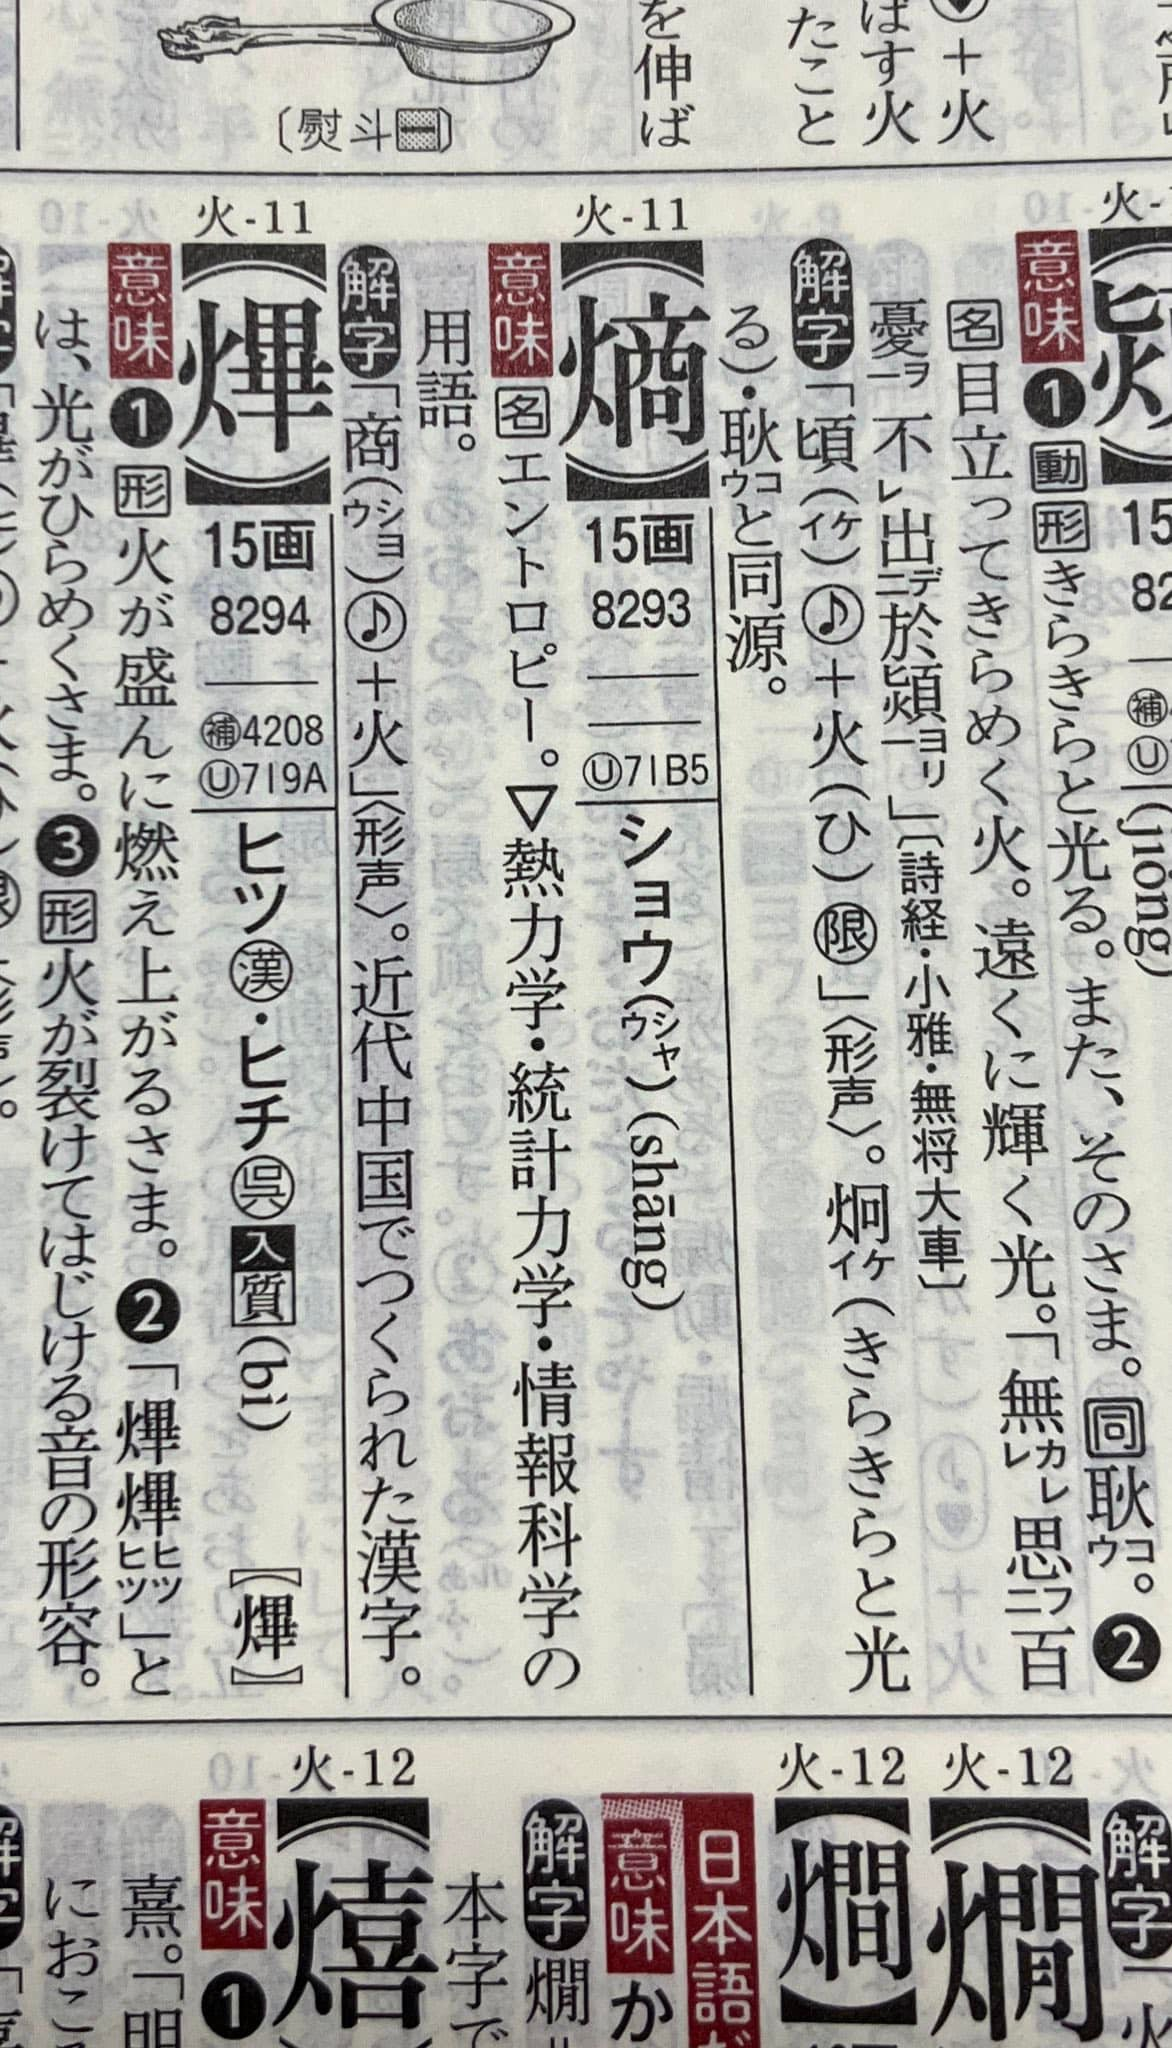
\includegraphics[width=\linewidth]{pictures/2024/07/20240730_123628_001.jpg}
\end{minipage}
\end{center}

\section{8月}

\subsection*{2024年08月03日 16:25}
\addcontentsline{toc}{subsection}{2024年08月03日 16:25}

「美しさに序列をつける」というのは奇妙な営みだ。

\url{https://x.com/haseryo_ME/status/1819526199888302158}




本当だ。言われてみれば、ちょっと奇妙な話だな。

音楽コンクール、絵画、書道、工芸などなど。それらに付けられる序列に対する客観的な根拠って何なんだろう。（「審査員の趣味」以上の根拠を示せるものなのだろうか？）見たり聴いたりした時に「胸を打たれる」様なことが起きる場合とそうでない場合があったとしても、それはその人の感情であって客観的とは思えないし、そもそも、皆んなが良いと思う作品って？即ち客観的に見て「よいもの」は、大概つまらないものである事が多い。（様な気がするだけ、かも知れないけど）ピカソやシャガール、モネなら「客観的」に良いものと言えるのか？客観性を求める事がそもそも誤りなんじゃないのか？しかし客観的でない視点によって付けられる序列が公にされ、その事に一喜一憂して、しかも多くの場合大多数が納得している様な気がするのは何故なのか？何らかの「権威の主観」による序列付けだからという事に過ぎないのか。

不毛なループに入り込んできている様な気がしてきた。（これは哲学だな）

\subsection*{2024年08月05日 03:27}
\addcontentsline{toc}{subsection}{2024年08月05日 03:27}

\paragraph{リンク}
\url{https://x.com/nhk_news/status/1819893272913100831}

\subsection*{2024年08月05日 22:07}
\addcontentsline{toc}{subsection}{2024年08月05日 22:07}

\#モーツァルト。アヴェ・ヴェルム・コルプス 素敵すぎる。


むかあーし（昔）の事だけど、ブラームスのドイツ・レクイエム（だったか？）のレコードを買ったら、後ろに、まるでアンコール曲の様にして収録されていた。短い曲だが、最後にこの曲を聞けば、心が慰められ穏やかになって、静かにレコードの針を収める事ができる。


コントラバスの合奏って一度も聞いた事なかったけど、こんな響きの中に浸っていたいものです。

（それにしても、「場所：Earth」とは、、、少し気になる）

\url{https://x.com/welovebassoh/status/1819989639723372998?s=61&t=5VtsOkpki6juEjPXsBq8hg}



\paragraph{写真}
\begin{center}
\begin{minipage}{0.48\linewidth}
\centering
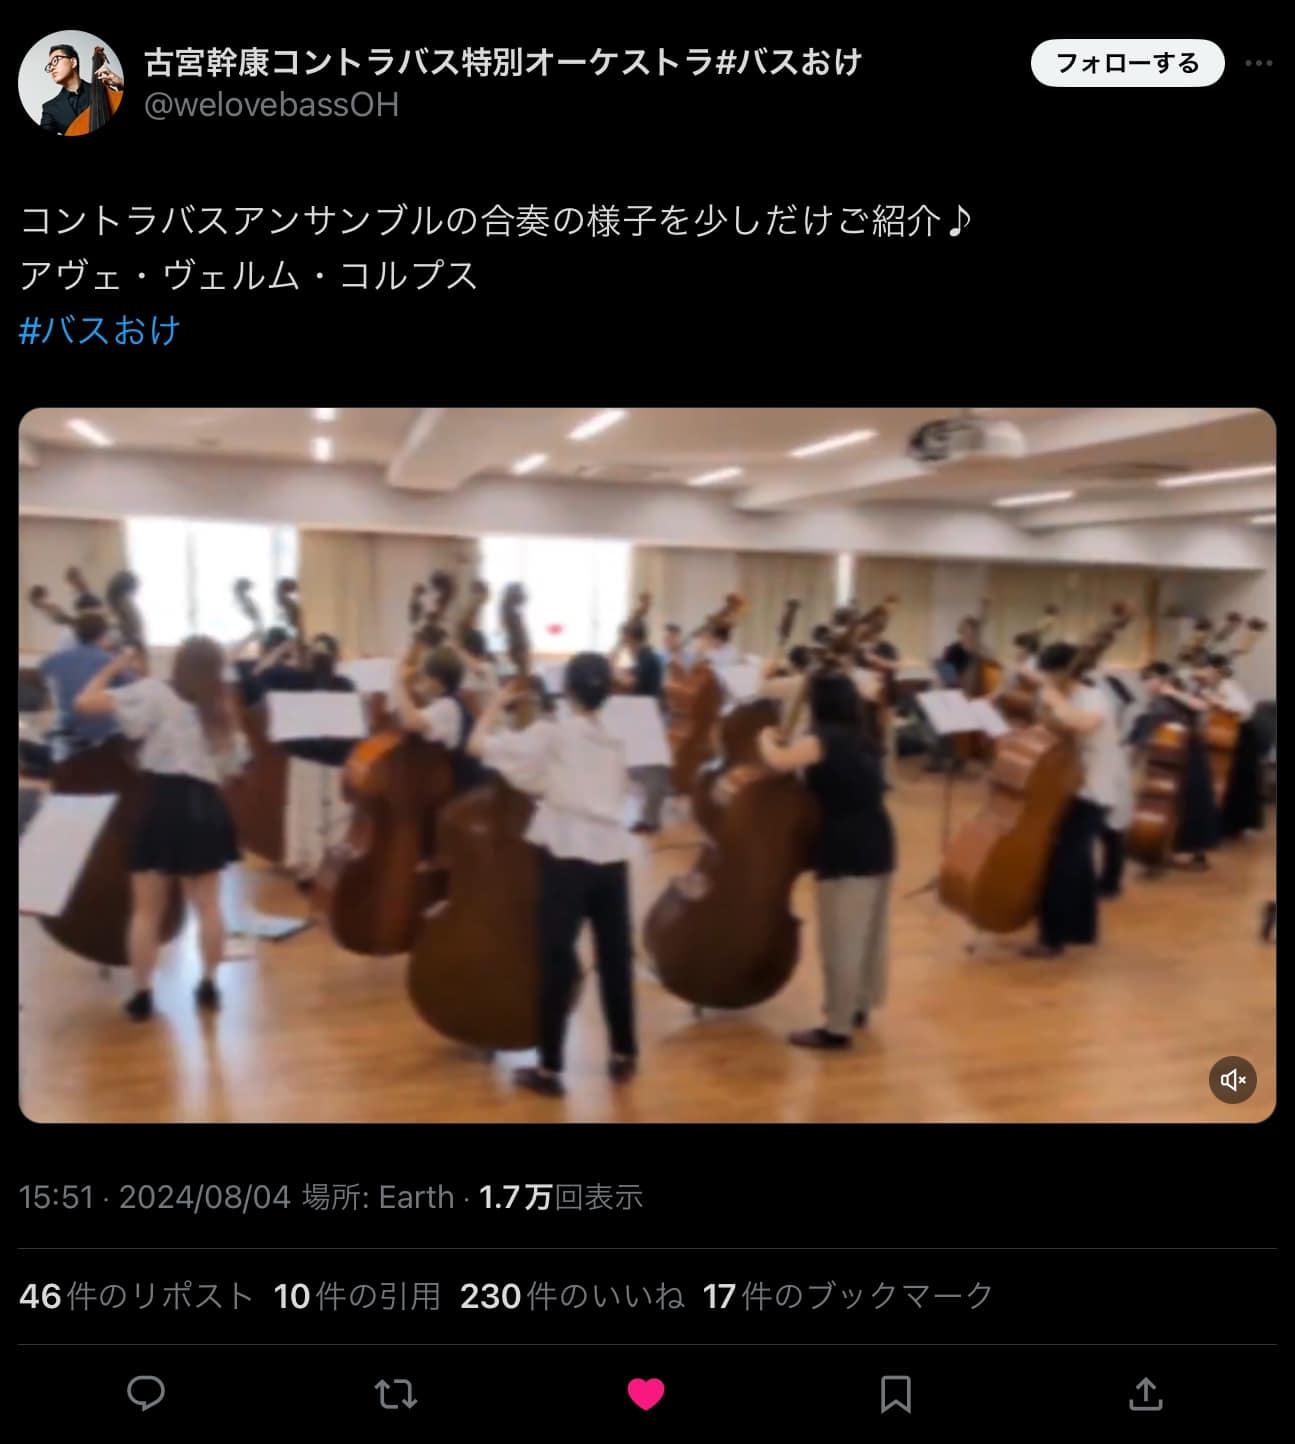
\includegraphics[width=\linewidth]{pictures/2024/08/20240805_220735_001.jpg}
\end{minipage}
\end{center}

\subsection*{2024年08月06日 17:25}
\addcontentsline{toc}{subsection}{2024年08月06日 17:25}

\url{https://m.facebook.com/groups/pythonclcoding/permalink/2292975087716093/}




興味深い。

そう言えばmatplotlibでもグラフのタイトルなどでTeXの記述を使えた。

さらにTeXのソースを生成してくれたらもっと嬉しい。

\paragraph{写真}
\begin{center}
\begin{minipage}{0.48\linewidth}
\centering
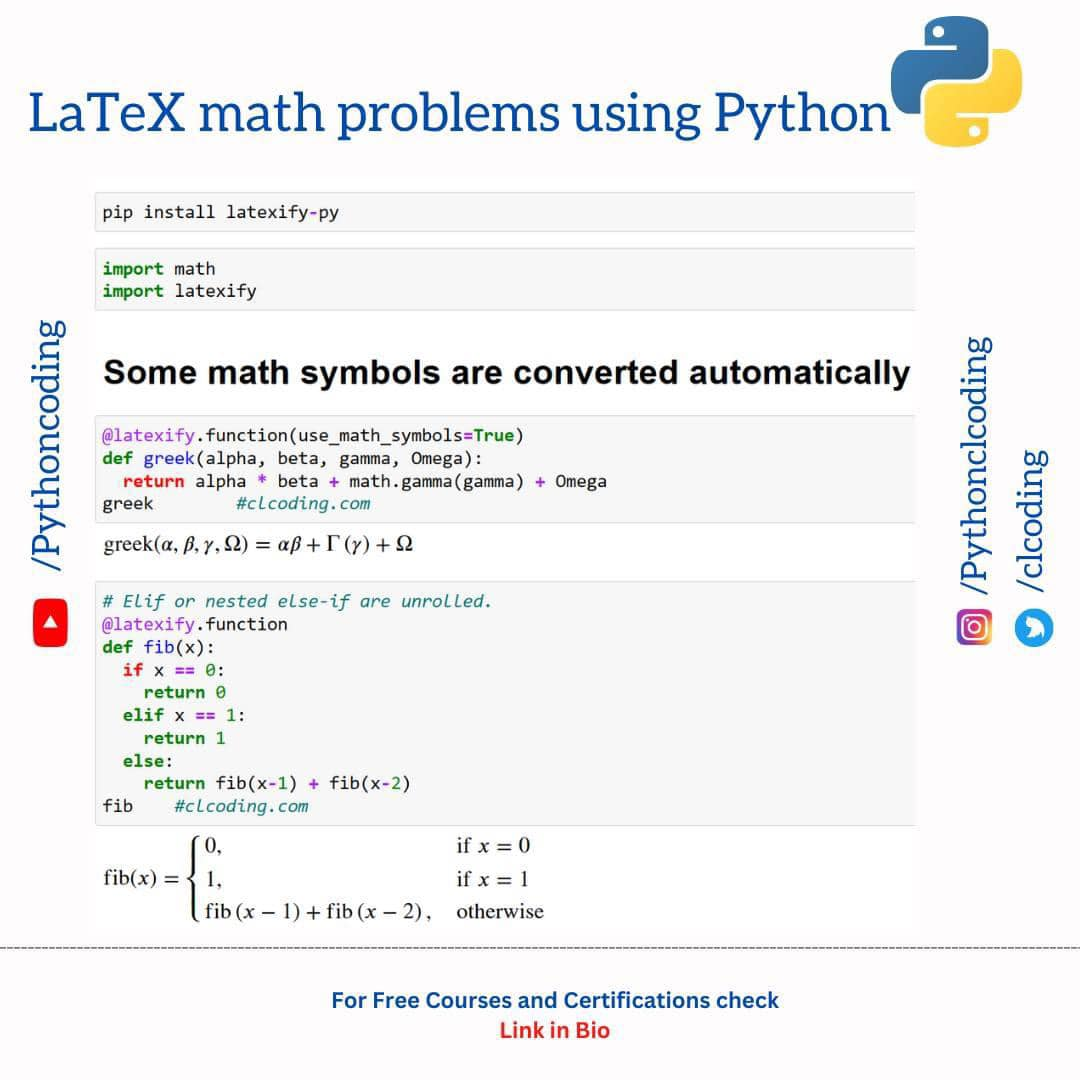
\includegraphics[width=\linewidth]{pictures/2024/08/20240806_172515_001.jpg}
\end{minipage}
\end{center}

\subsection*{2024年08月09日 07:18}
\addcontentsline{toc}{subsection}{2024年08月09日 07:18}

\#井上ひさし 氏の「\#母と暮せば」。今日（8/9）の「\#天声人語」では \#山田洋次 監督による映画に言及しているが、氏の志は舞台（\#こまつ座）でも引き継がれている。


The tragedies of August 6 and 9 were not inevitable or fated. We humans could have avoided the atomic bombings. Because those terrible tragedies were planned and carried out by human beings.

\paragraph{写真}
\begin{center}
\begin{minipage}{0.48\linewidth}
\centering
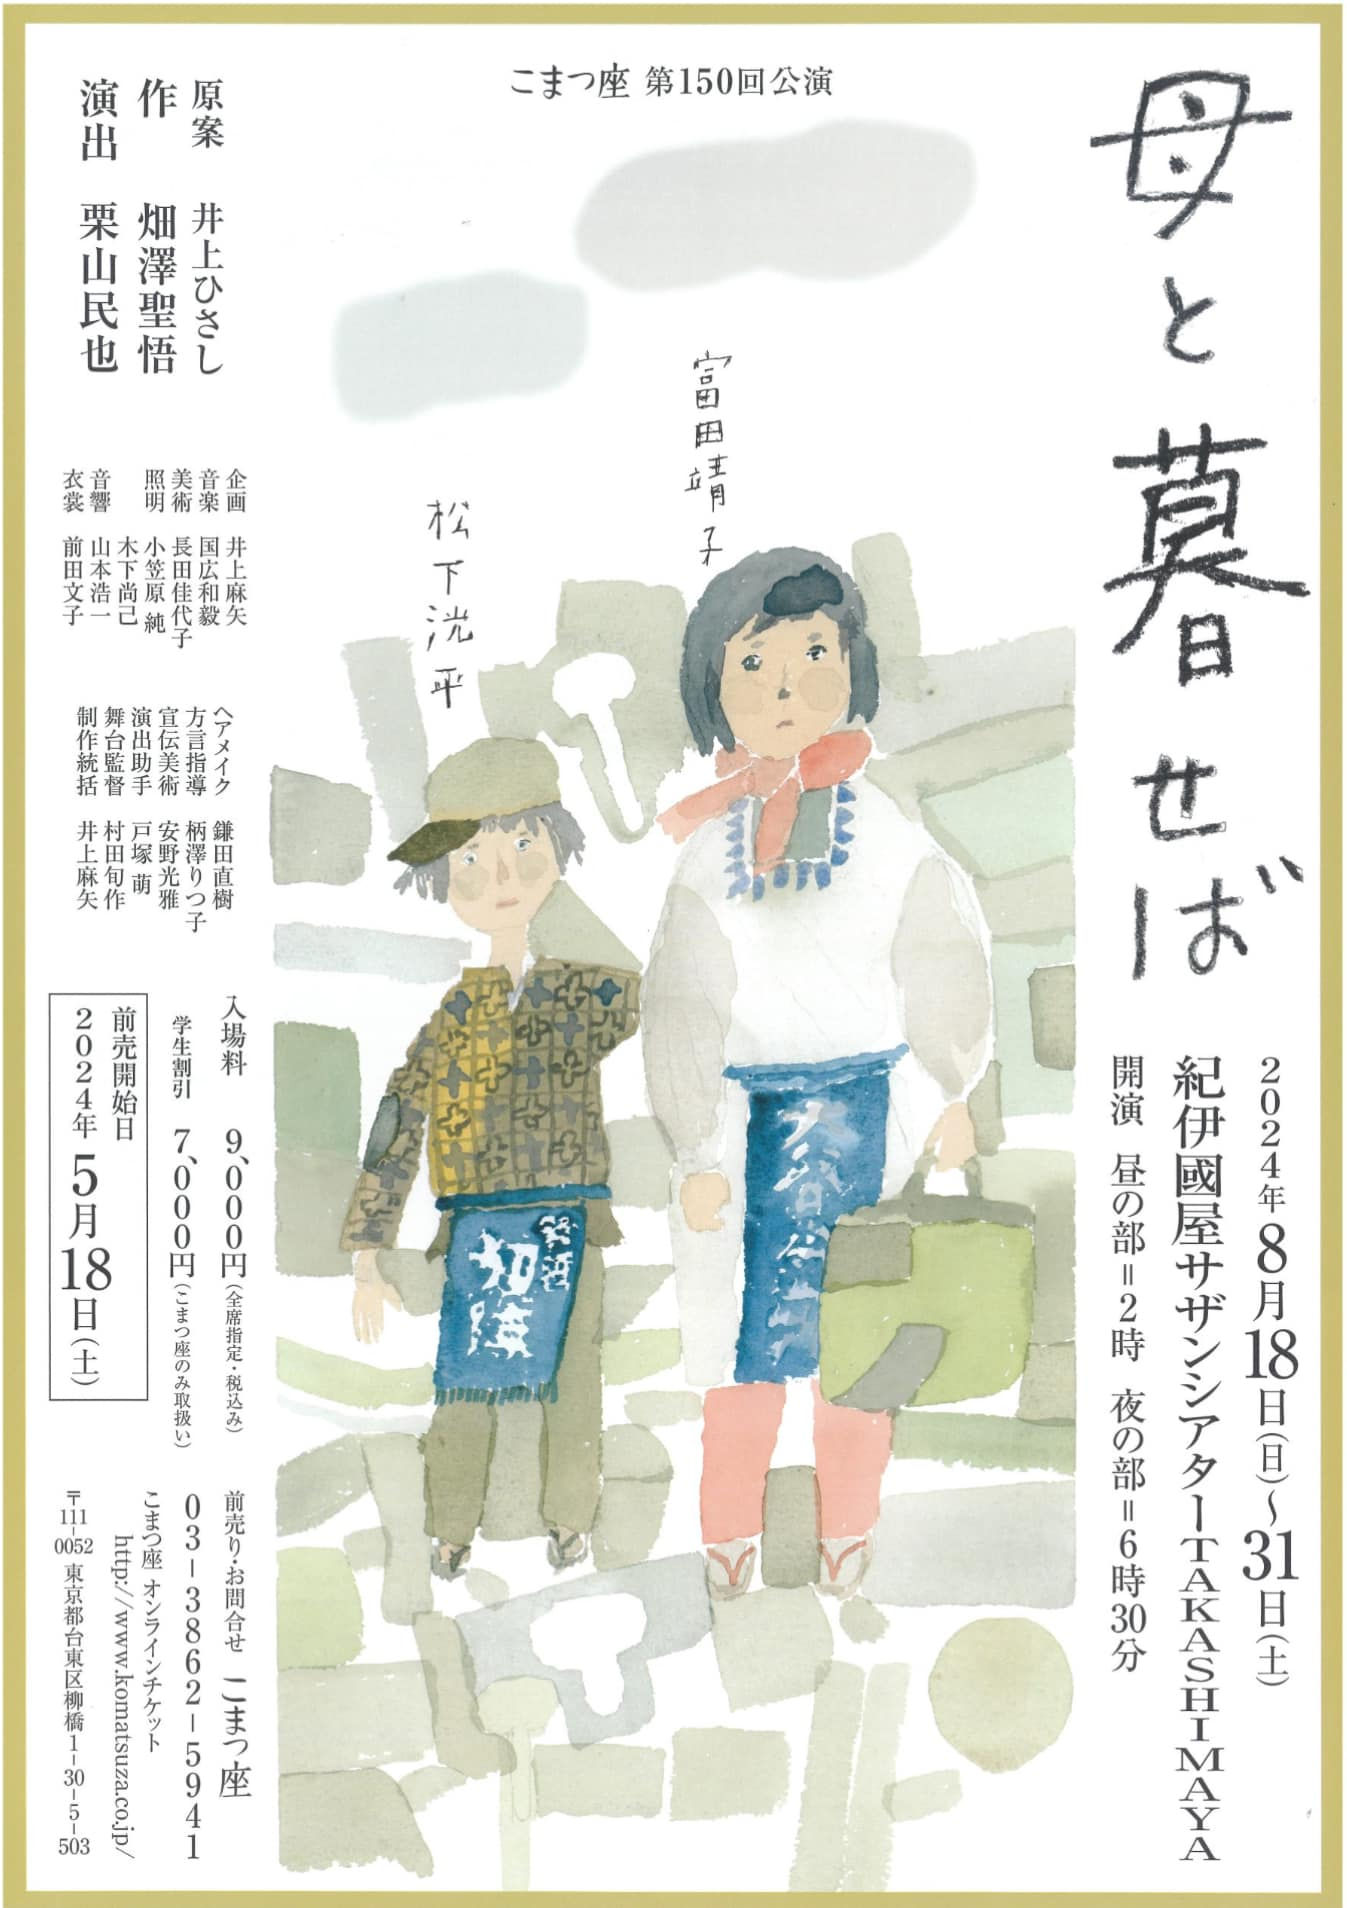
\includegraphics[width=\linewidth]{pictures/2024/08/20240809_071802_001.jpg}
\end{minipage}
\end{center}

\subsection*{2024年08月09日 09:44}
\addcontentsline{toc}{subsection}{2024年08月09日 09:44}

\url{https://www.yomiuri.co.jp/pluralphoto/20240803-OYTAI50010/}




「インターハイのバレーボールで高校生審判、記録係」こういうのはすごく嬉しい。こうあるべきなんだと思う。


むかーし（昔）から強く疑問に思っている事は「ブラスバンドの指揮者をなぜ生徒にやらせないのか」という事です。曲作りが教員による生徒への押しつけの様になっているのではないか？本来なら生徒が享受するべき「曲作り」に関する学びを、教員が指揮者の立場を占有することによって、生徒から奪ってしまっているのではないのか？そもそも「曲作り」は生徒に委ねるのが望ましいのではないかと考えているのです。

理想を言えば、指揮者の生徒を中心としてメンバで話し合って、曲のイメージを共有したり、表現を自分たちで納得して決めていくようになると良いと思います。でも、それはとても難しいことで、教員が「決めて指示して（強制して）」進めた方が効率良いことなのでしょうね。

それでも、やっぱり生徒自身が曲作りをする「方向に導いていく」ことはできないものでしょうか。仮にその事によって結果として比較的完成度の低い演奏になったとしても、です。あそこはああすれば良かった、あの時こうしていたら良かった。こういう事が足りていなかったんだ、そんな表現もあったのか。そういった事に気づかざるを得なくなった時、その時こそ、音楽の表現、曲作りに関する学びを獲得するタイミングなのではないかと思うのです。

先生に言われた通り（盲目的？）に指を動かす訓練（演奏？）をしていたとして、生徒の視点は極めて近視眼的であり、曲全体の「曲作り」関して、ああしたら、こうしたらという視点は持ち得ないことでしょう。「先生に言われた通りに、厳しい毎日の練習や訓練に耐えてきました」ではなくて、「自分たちでゼロから曲を作りあげてきたんだ」という、そんな気にさせる事は出来ないものでしょうか。

吹奏楽コンクールで、次の学校もその次の学校も「生徒が」指揮台に上がってきて、若い爽やかな曲作りを響かせる。(テンポが速かったり、ディナーミク、アゴーギクが大袈裟だったり。そんなことって、普通だったら起きるものなんじゃないの？)そんな個性的な表現を聞きたいと思うのは私だけなのでしょうか。（おじさんおばさん（教員）が指揮台の上で意気がって棒を振っていて、CDのコピーみたいな演奏が次々と行われていくのって、どうなんだろうか？)

現実（現場）から目を背けているかもしれません。自分が考える理想だけを言い放っているのかもしれません。（せいぜい年寄りの独り言に過ぎないとして聞き流してほしい所です）

\paragraph{写真}
\begin{center}
\begin{minipage}{0.48\linewidth}
\centering
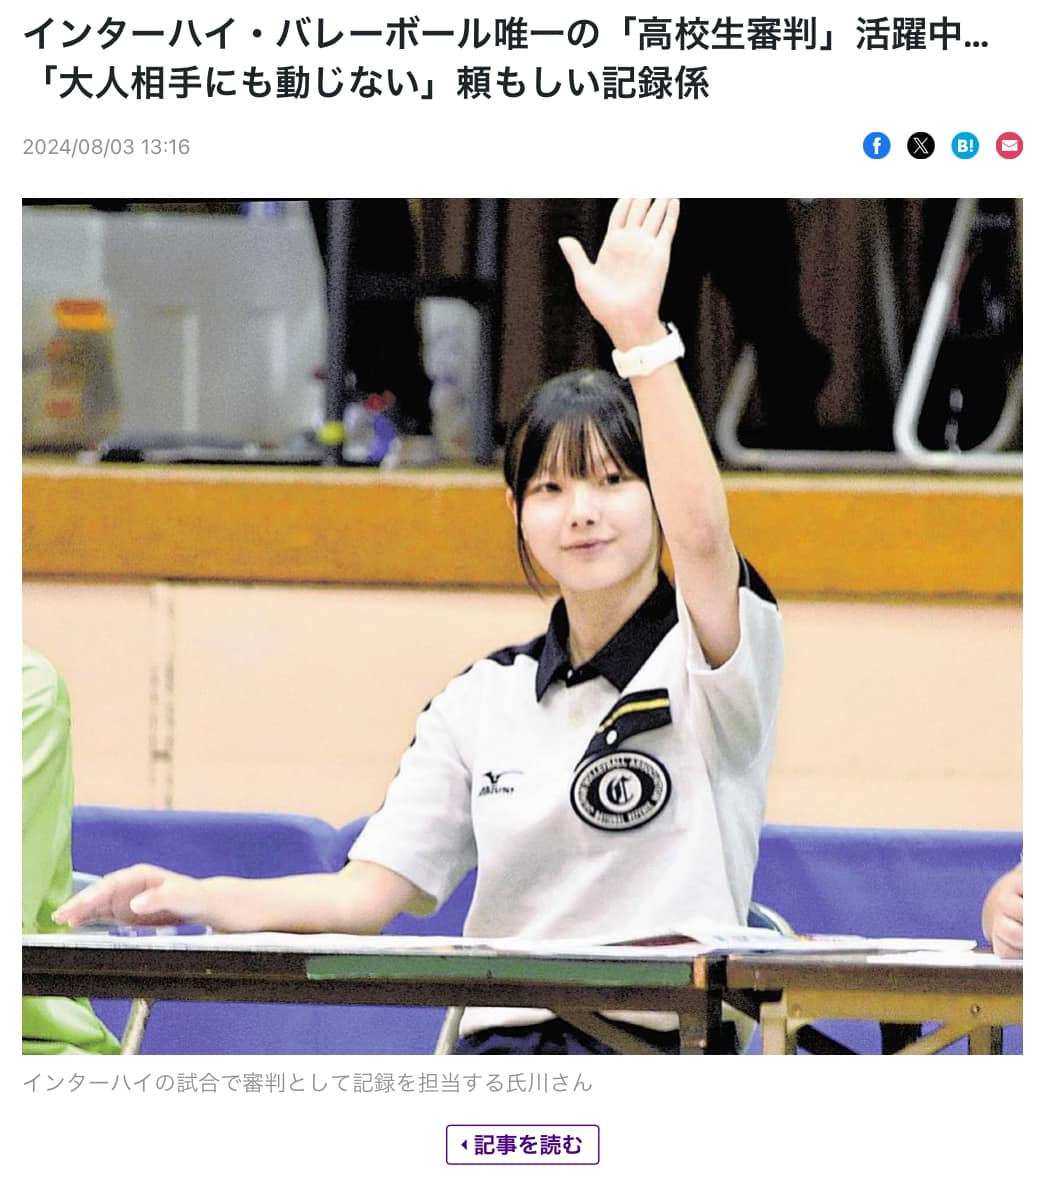
\includegraphics[width=\linewidth]{pictures/2024/08/20240809_094445_001.jpg}
\end{minipage}
\end{center}

\subsection*{2024年08月10日 19:00}
\addcontentsline{toc}{subsection}{2024年08月10日 19:00}

\url{https://m.facebook.com/story.php?story_fbid=1182866802781219&id=100031737316033}




今日（8/10）の第二回を聴講しました。


(１)

ト音記号、フランス式では第一線がG（第二線がGなのはイタリア式）

(２)

4分の4拍子のCマークと、縦棒の入っているCマーク。速さの違いにもなっていて、同じ楽譜が全く違ったニュアンスの曲になる。

(３)

Handel G-dur の2楽章を例に話されていた、タンギングによるアーティキュレーションの話は最高に面白かった。この曲を以前演奏した時に「どう切ったらいい？」と少しだけ試行錯誤してみていた事を思い出しました。できればHandelのe-mol（HWV359b）の2楽章もアーティキュレーションの説明あると嬉しいんだけどなぁ。

(４)

例えばタンギングを、t r t t r t なんてしたら、それだけで「スラー+スタッカート」をイメージしてしまう。おおよそ、「タンギング＝アーティキュレーション」というと言い過ぎなのだろうか？アーティキュレーションを「歌って」いると、それがタンギングになっている（笛の音に結びついている）としたら、つまり「歌う様に笛を吹いている」状況になっているわけで、何だか素敵な楽器だなぁという気がする。

(５)

アウフタクトの後の小節の頭の急降下「たわみ」の話も面白かった（有田先生はナイキのマークみたいなとおっしゃった事がありました）J.S.Bachの無伴奏の出だしの所の例も興味深いものでした。


＃前田りり子 \#トラヴェルソ \#Quantz \#クヴァンツ \#フルート奏法


⚪︎第一回目の聴講

\url{https://m.facebook.com/story.php?story_fbid=7876849065732519&id=100002225117991}



\subsection*{2024年08月13日 19:53}
\addcontentsline{toc}{subsection}{2024年08月13日 19:53}

\url{https://youtu.be/-b1nq3425oM}

\begin{center}
\href{https://youtu.be/-b1nq3425oM}{
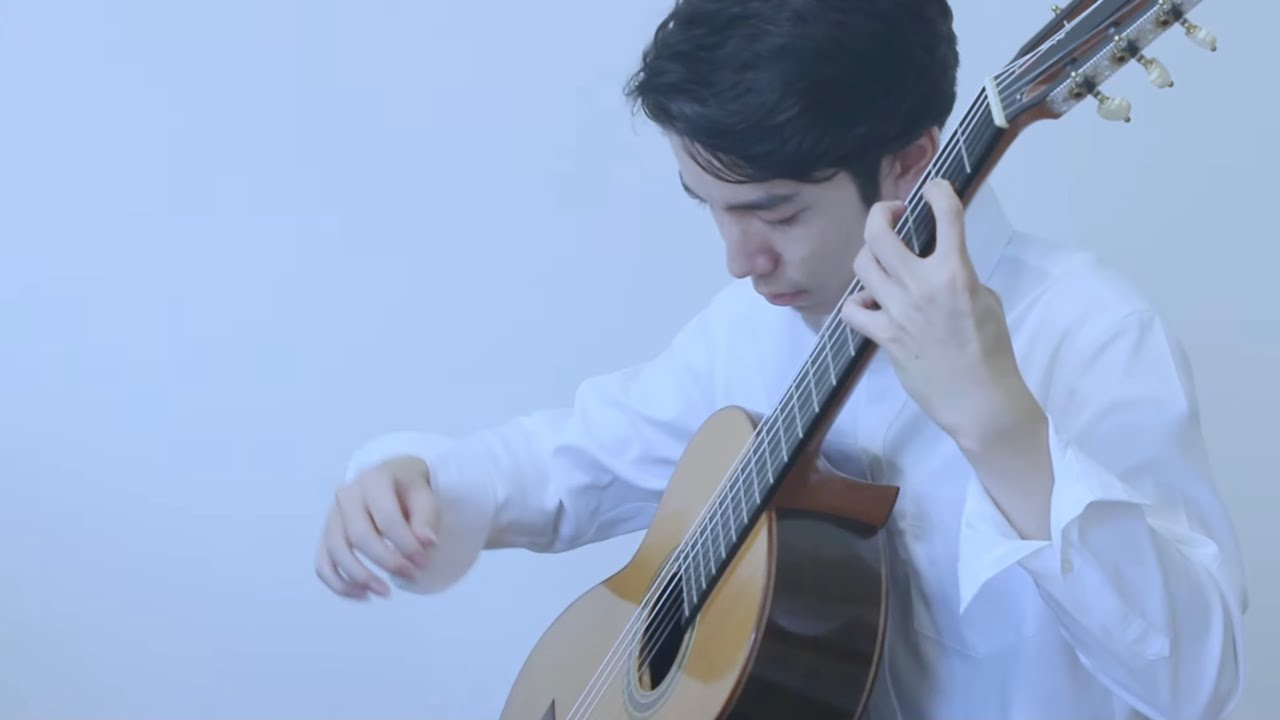
\includegraphics[width=0.48\linewidth]{pictures/youtube/2024/08/20240813_195308_youtube_001_-b1nq3425oM.jpg}
}
\end{center}



「\#波の盆」


\#武満徹：作曲

\#鈴木大介：ギター編曲

\#岡本拓也：演奏


昭和の映画音楽にも大きな足跡を残した武満徹です

ユダヤをルーツとする人には、マーラーに強い共感を覚える方がいると聞きます（例えば、レナード・バーンスタイン）

一方、武満のサウンドに何とも言えない郷愁の様な気持ちを感じてしまうのは、（日本人の）私だけでしょうか？

\subsection*{2024年08月15日 14:00}
\addcontentsline{toc}{subsection}{2024年08月15日 14:00}

江戸時代には \#金沢城 と \#兼六園 を結ぶ土手の橋であった \#石川橋 は、橋の下の広坂側を \#百間堀 、兼六園下交差点側を \#白鳥堀 と呼ぶ水堀だったそうです｡（

\url{https://www.siro-niwa.com/_wp/3391/}

）


\#石川県立歴史博物館 および \#加賀本多博物館 の裏手（殆ど職員駐車場になっている様だが）には、平成七年に建て替えられる以前の石川橋の一部（残骸？）が置かれているのを発見！してしまいました。（添付写真の通り。展示してあると言うより、隅っこに置いてあるという雰囲気。）現在の石川橋の親柱には「平成七年三月架」となっていますが、この残骸には「明治四十四年三月架」となっています。


「石川橋の高欄」というプレートには、「城下町金沢が近代化する際に、旧城下の中心部を横断する都市計画道路の敷設に際して建設された石川橋の一部である。この百間堀開削道路は、明治44年（1911年）6月開通。幅6間、延長317間、路肩部に公園を付随した近代的な道路で、その間に石川門と兼六園を結ぶ幅30尺の陸橋（石川橋）が設けられた。同陸橋は、石川県における鉄筋コンクリート建造物の初期の事例でもあり、街灯の意匠などに明治期の特徴をよく残している。」と書かれています。


この橋が平成七年に建て替えられる前までは、1911年（明治四十四年）に作られた鉄筋コンクリート製の橋というのは、琵琶湖疏水の橋（1903年製）に次ぐ、日本で２番目の古さだったとの事です。

\url{https://m.facebook.com/story.php?story_fbid=998254088759437&id=100057245658757}



\paragraph{写真}
\begin{center}
\begin{minipage}{0.48\linewidth}
\centering
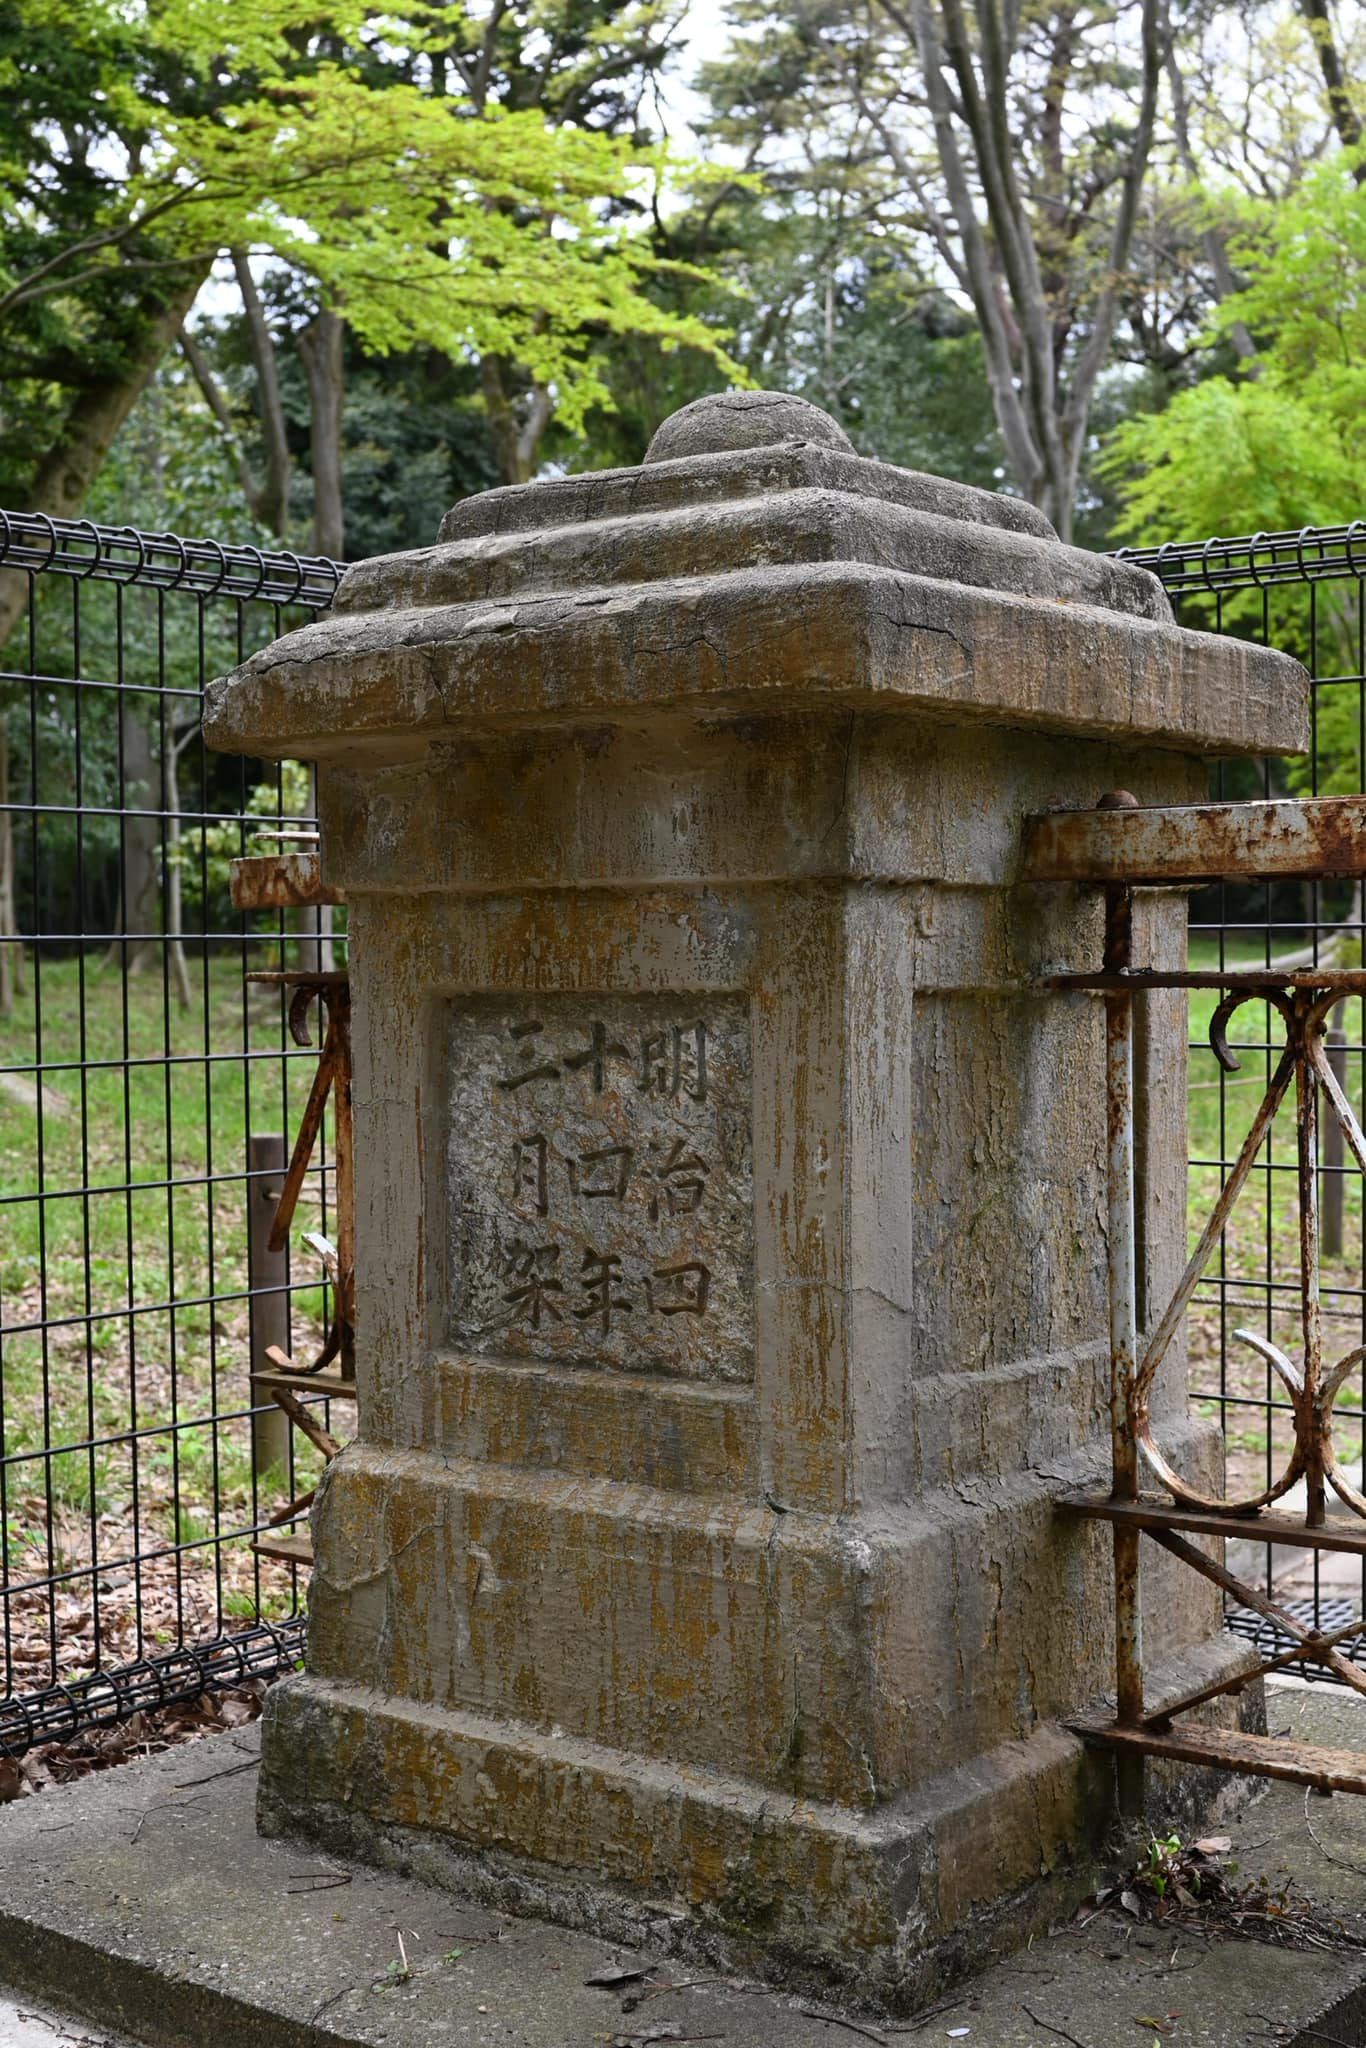
\includegraphics[width=\linewidth]{pictures/2024/08/20240815_140010_001.jpg}
\end{minipage}
\hfill
\begin{minipage}{0.48\linewidth}
\centering
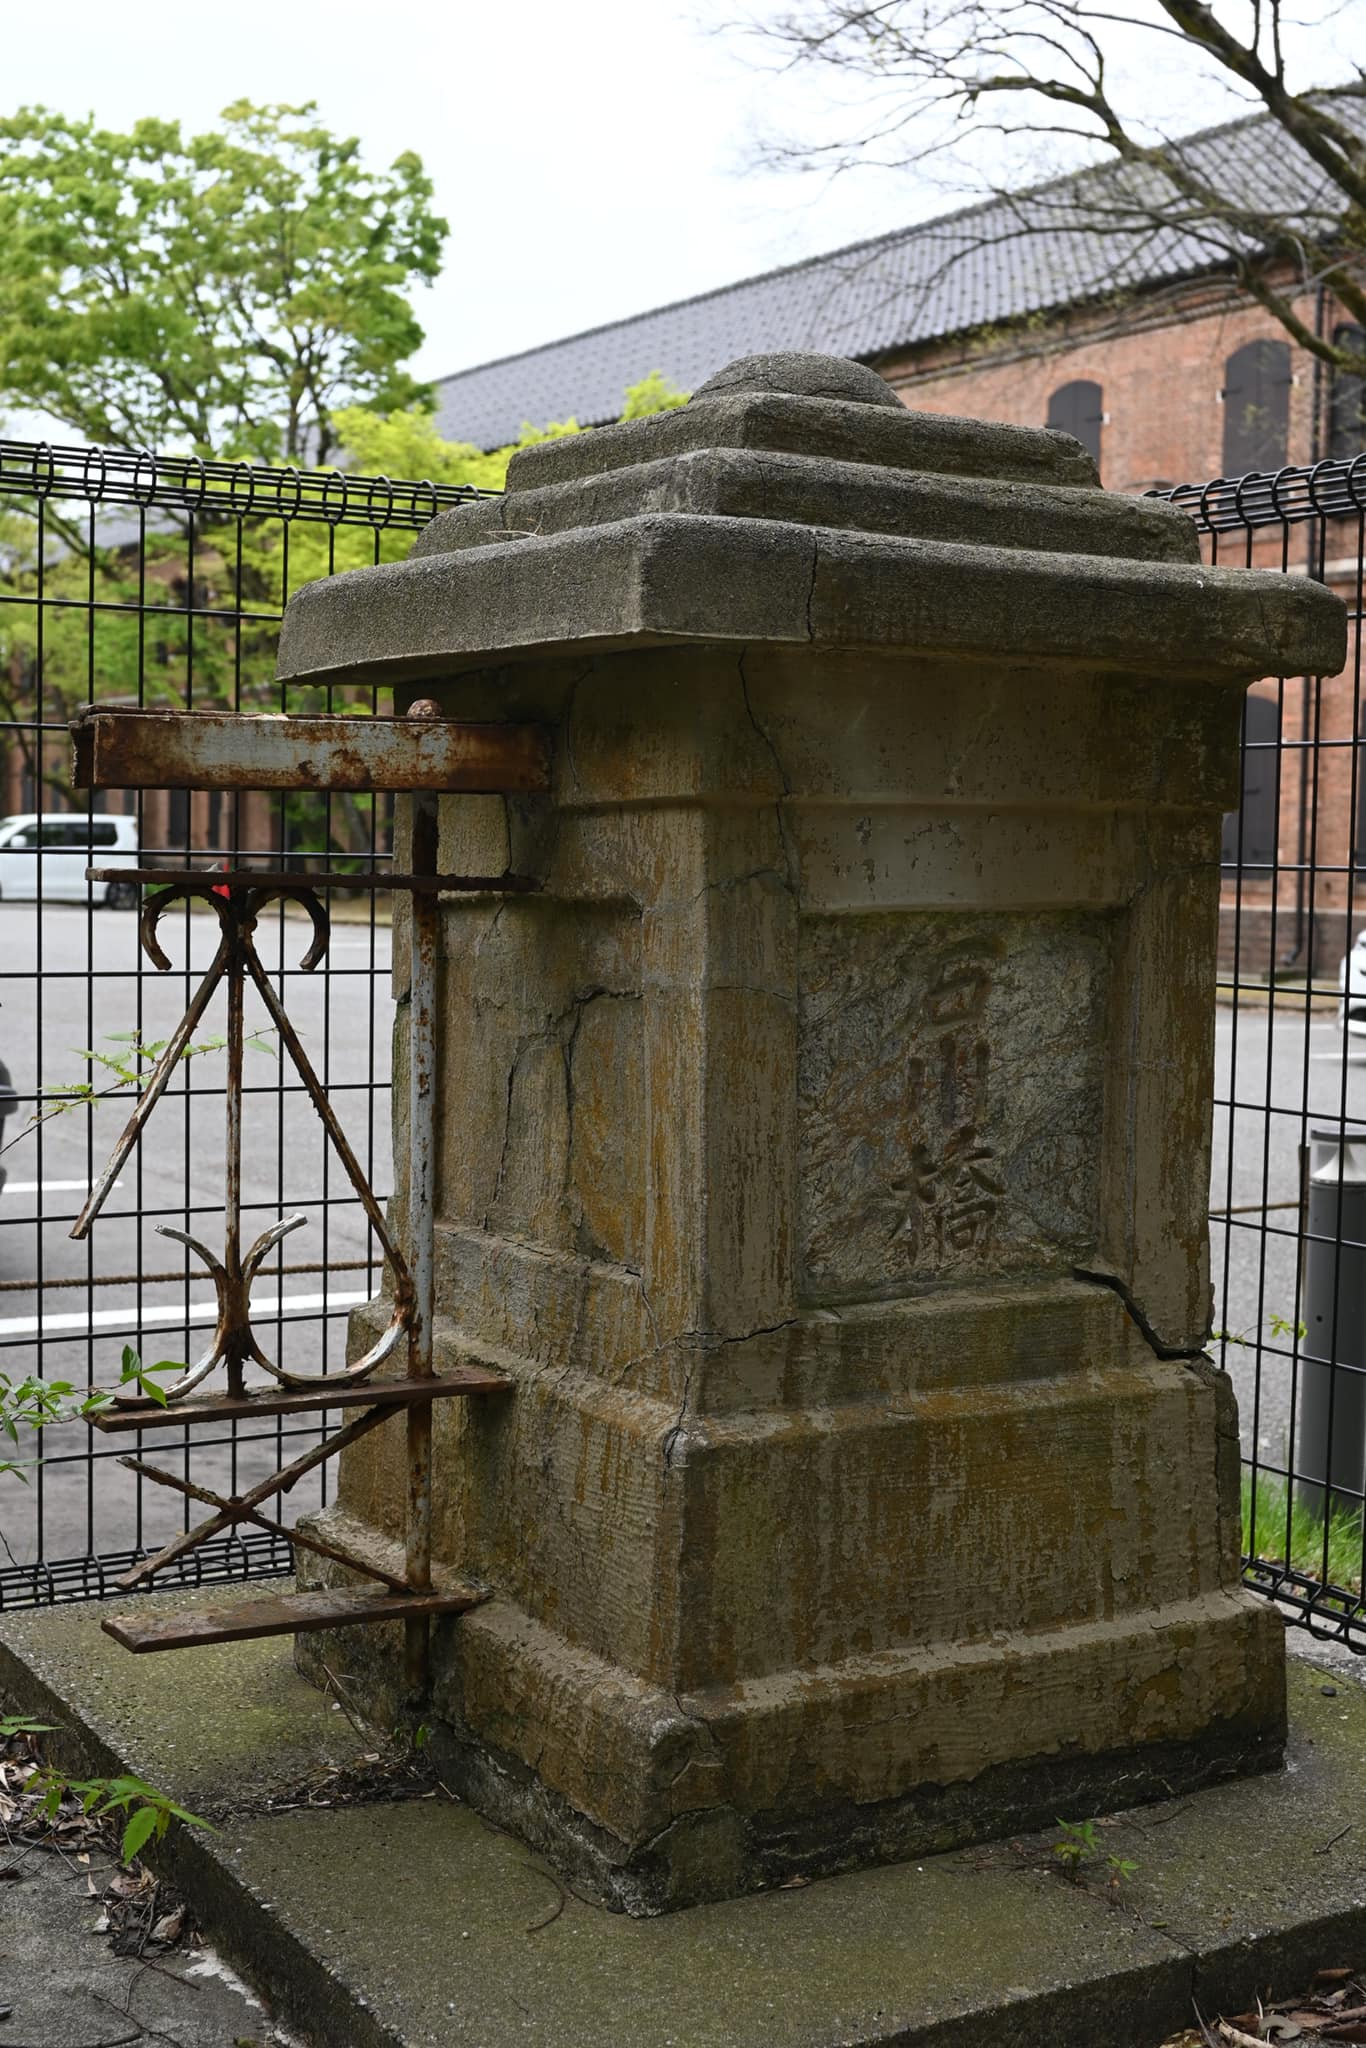
\includegraphics[width=\linewidth]{pictures/2024/08/20240815_140010_002.jpg}
\end{minipage}
\end{center}

\begin{center}
\begin{minipage}{0.48\linewidth}
\centering
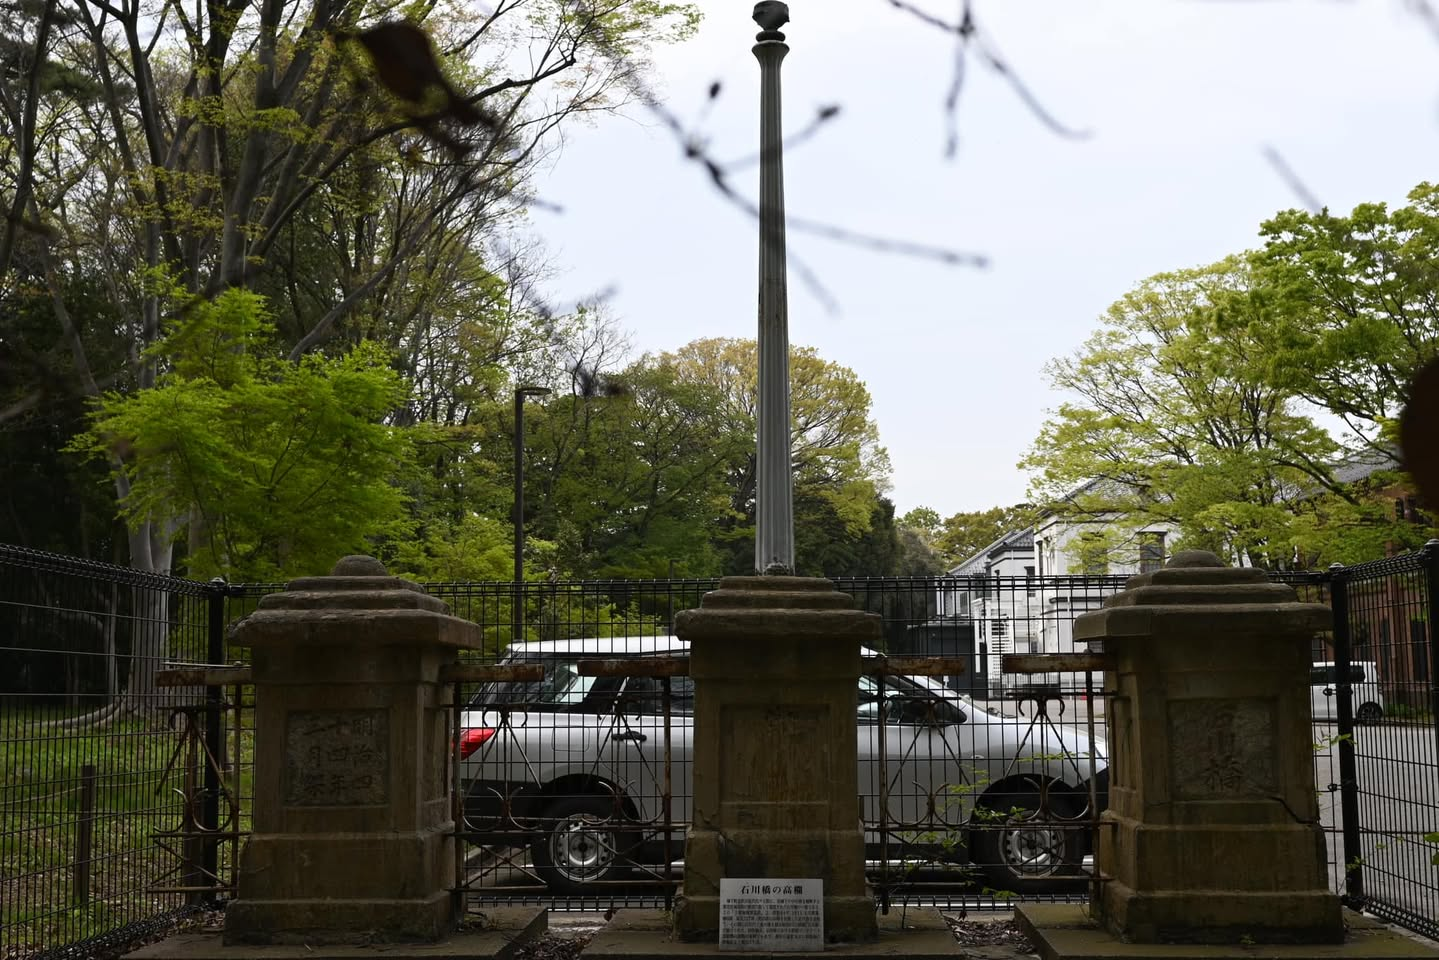
\includegraphics[width=\linewidth]{pictures/2024/08/20240815_140010_003.jpg}
\end{minipage}
\end{center}

\subsection*{2024年08月17日 09:49}
\addcontentsline{toc}{subsection}{2024年08月17日 09:49}

\paragraph{リンク}
\url{https://x.com/haseryo_ME/status/1819526199888302158}

\subsection*{2024年08月17日 17:11}
\addcontentsline{toc}{subsection}{2024年08月17日 17:11}

ラヴェルやドビュッシーの歌曲（メロディー）を天才 \#矢野顕子 氏が「英語で」歌っている。ピアノ伴奏は \#高橋悠治 氏。フランス語でなくても大丈夫。むしろ楽曲に新たな価値が追加された格好だ。歌にどんどん引き込まれる。本当に天才の所業（歌唱）と言う他ないよ。（シューベルトのリート、\#谷川俊太郎 作詞で高橋悠治作曲の歌曲も入っている。矢野顕子氏はシンガーソングライターだが、このアルバムでは歌い手に徹している様だ）


🎧lnk.to/u9xjcnNh

\paragraph{写真}
\begin{center}
\begin{minipage}{0.48\linewidth}
\centering
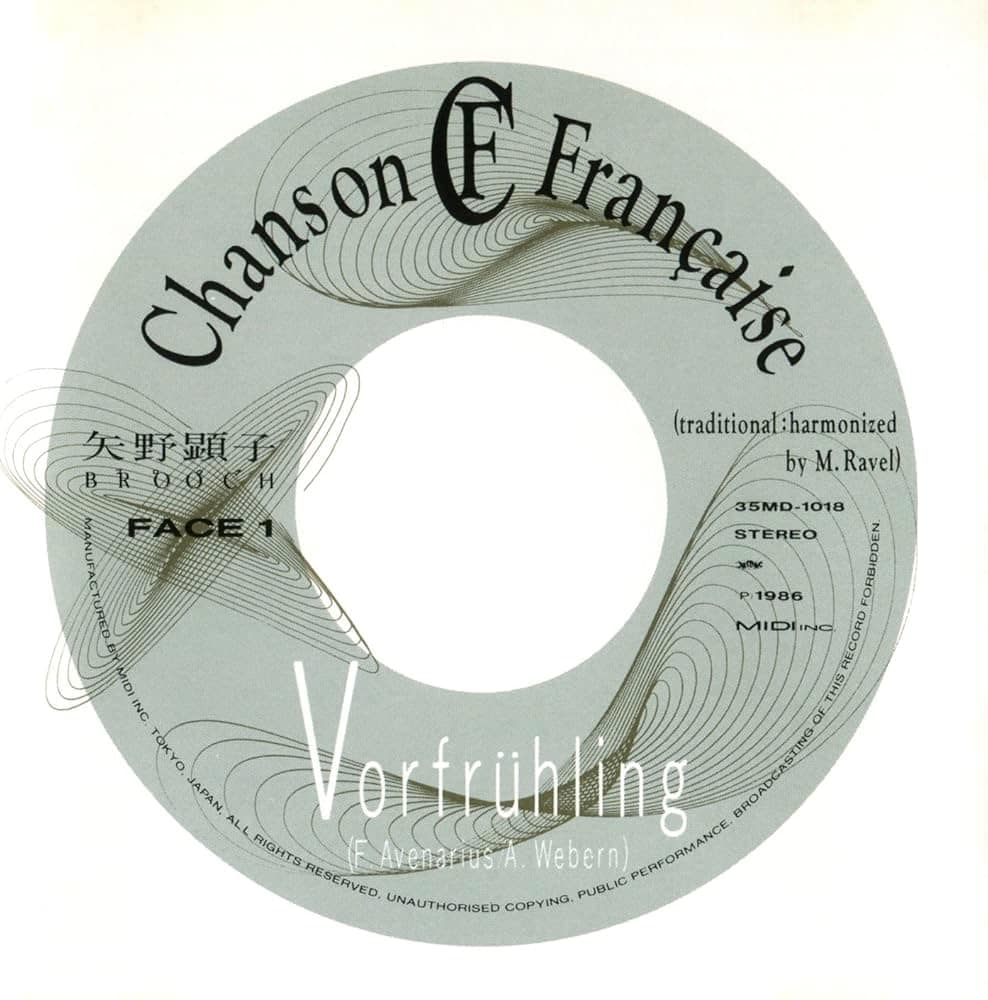
\includegraphics[width=\linewidth]{pictures/2024/08/20240817_171113_001.jpg}
\end{minipage}
\end{center}

\subsection*{2024年08月20日 07:01}
\addcontentsline{toc}{subsection}{2024年08月20日 07:01}

\paragraph{リンク}
\url{https://kanazawasaka.com/column/tsurumazaka-yurai-01.html}

\subsection*{2024年08月23日 02:46}
\addcontentsline{toc}{subsection}{2024年08月23日 02:46}

\paragraph{リンク}
\url{https://ameblo.jp/kanazawa-saihakken/entry-11113106101.html}

\subsection*{2024年08月23日 09:06}
\addcontentsline{toc}{subsection}{2024年08月23日 09:06}

応援中: 金沢 ―トップファンに認定されました！🎉

（「金沢」さんが発信されている情報のファンの一人である、という様な意味か。）

\paragraph{写真}
\begin{center}
\begin{minipage}{0.48\linewidth}
\centering
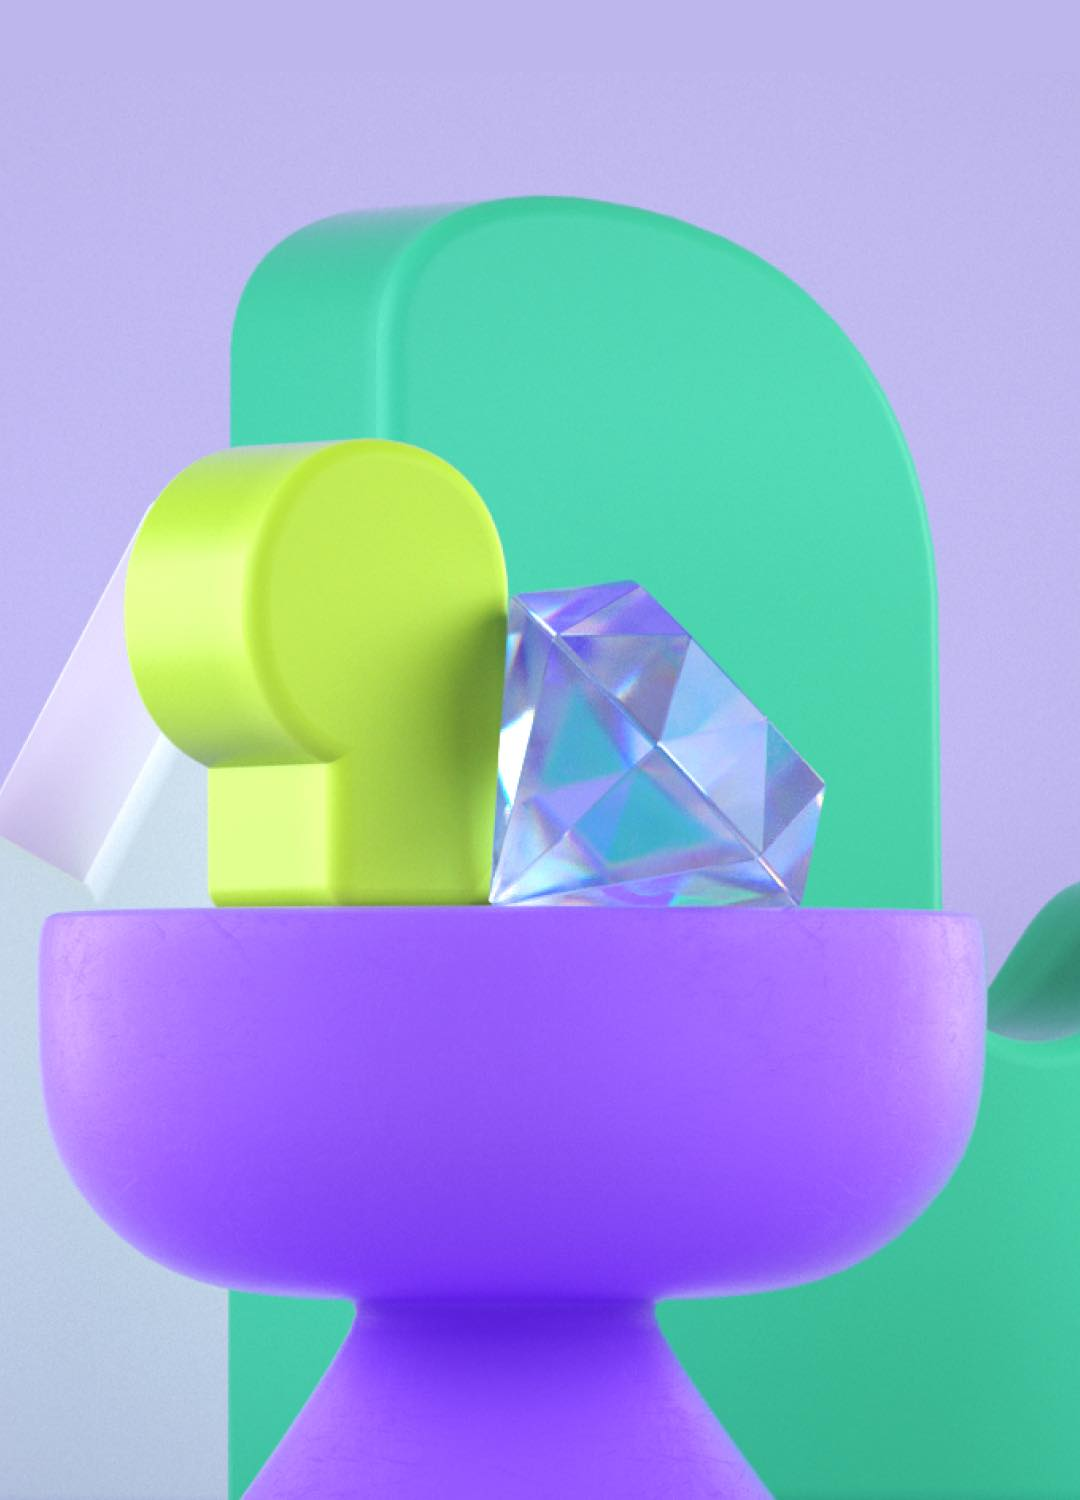
\includegraphics[width=\linewidth]{pictures/2024/08/20240823_090618_001.jpg}
\end{minipage}
\end{center}

\subsection*{2024年08月23日 11:01}
\addcontentsline{toc}{subsection}{2024年08月23日 11:01}

応援中: Frans Brüggen ―ライジングファンに認定されました！🎉

\paragraph{写真}
\begin{center}
\begin{minipage}{0.48\linewidth}
\centering
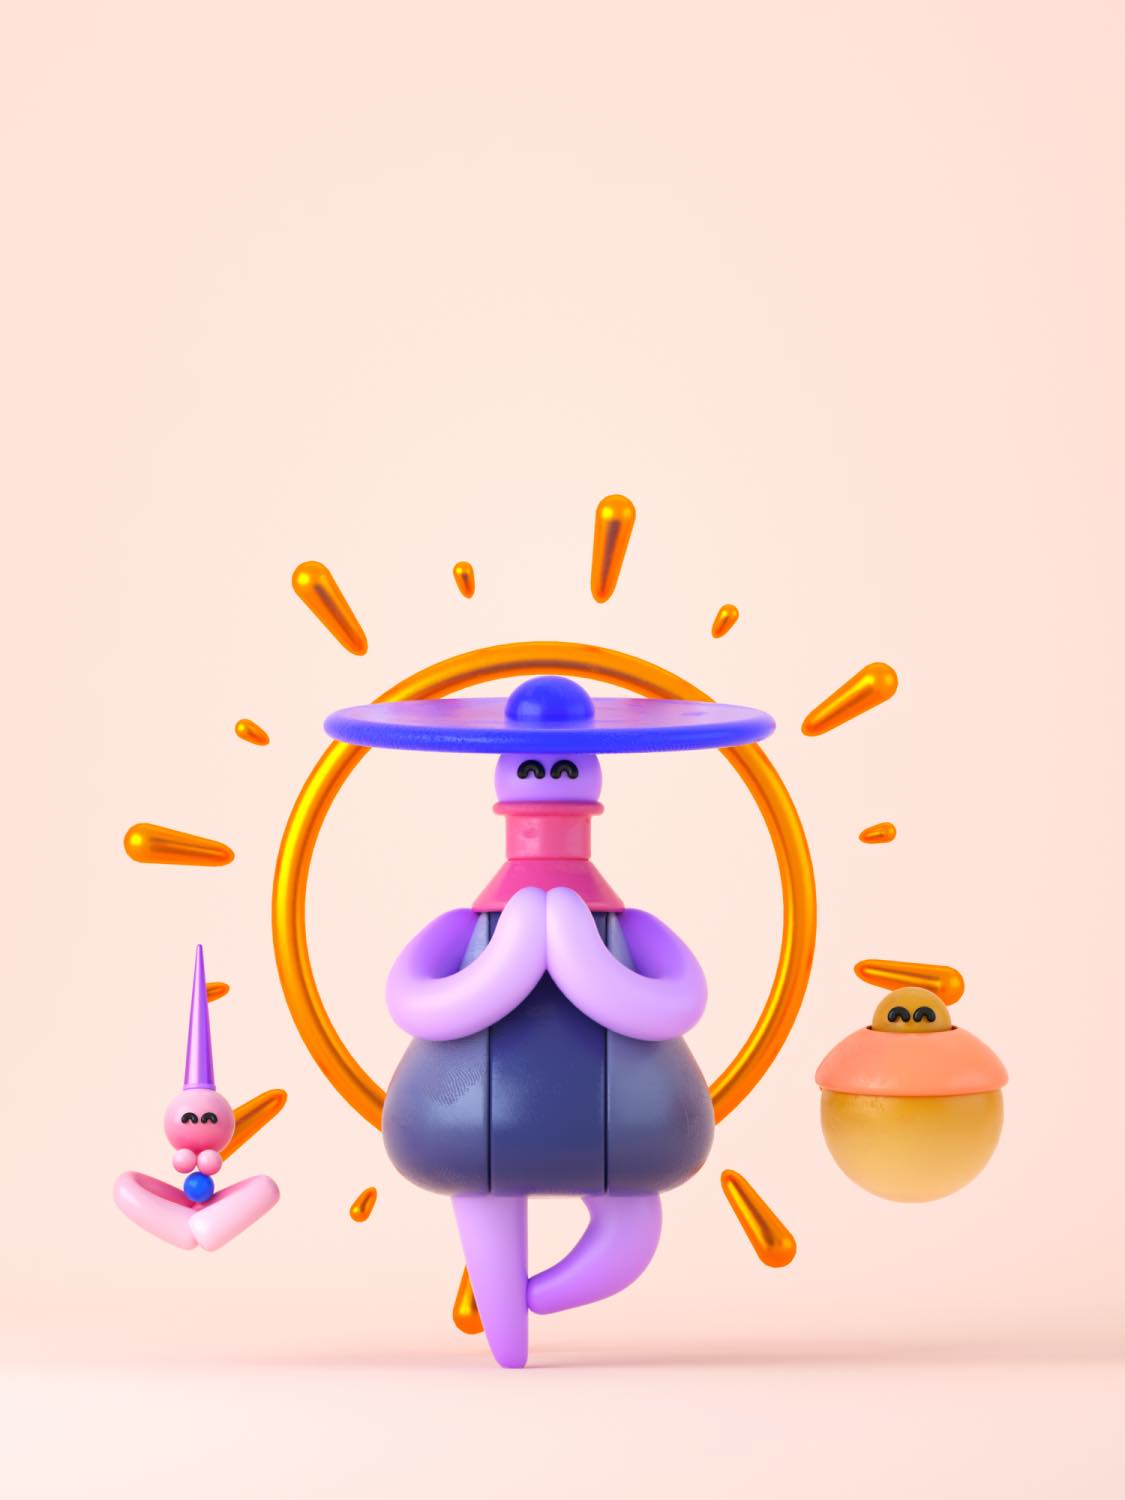
\includegraphics[width=\linewidth]{pictures/2024/08/20240823_110121_001.jpg}
\end{minipage}
\end{center}

\subsection*{2024年08月25日 08:59}
\addcontentsline{toc}{subsection}{2024年08月25日 08:59}

\paragraph{リンク}
\url{https://www3.nhk.or.jp/sapporo-news/20240820/7000069204.html}

\subsection*{2024年08月25日 18:58}
\addcontentsline{toc}{subsection}{2024年08月25日 18:58}

\url{https://fb.watch/uaKsj5bs-C/}




大地の歌Das Lied von der Erde（The Song of the Earth）のラストだ。


弦のユニゾンcresc..<<<<…その後dim.>

一本の絹糸の様に張りつめる緊張！そのままためておいて。。。。。

（ここでバーンスタインがクリスタ.ルートヴィヒに「入れ」のアインザッツ！）

そしてっ、


「ディー．リーベ．エールデ（Die liebe Erde） …」

…….

「ewig, ewig, …., ewig, ewig, ….」ひたすらdim. >>>>….


ああ、美しい大地は永遠に続いていく。。。

（エーヴィッヒ、〜エーヴィッヒが頭の中で鳴り続ける）


と言う事で。酒だ酒だ！お酒を飲もおっと。

（「酒持って来い！」などとは言えない。）

Laßt mich betrunken sein!

Dunkel ist das Leben, ist der Tod!

\subsection*{2024年08月26日 20:55}
\addcontentsline{toc}{subsection}{2024年08月26日 20:55}

\paragraph{リンク}
\url{https://4skills.im-kobetu.com/}

\subsection*{2024年08月27日 18:14}
\addcontentsline{toc}{subsection}{2024年08月27日 18:14}

\paragraph{リンク}
\url{https://youtu.be/p_RkX25i1PE}

\begin{center}
\href{https://youtu.be/p_RkX25i1PE}{
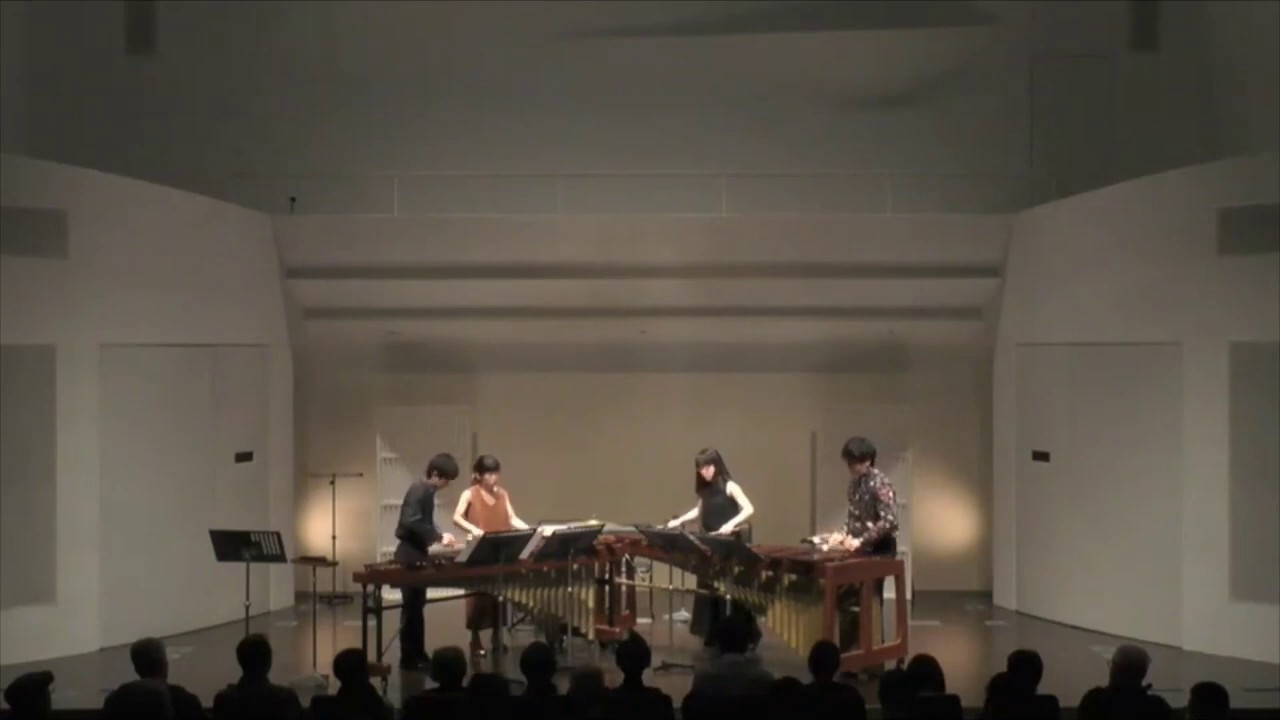
\includegraphics[width=0.48\linewidth]{pictures/youtube/2024/08/20240827_181450_youtube_001_p_RkX25i1PE.jpg}
}
\end{center}

\subsection*{2024年08月27日 23:16}
\addcontentsline{toc}{subsection}{2024年08月27日 23:16}

\paragraph{リンク}
\url{https://youtu.be/gDKCK_6WLTg}

\begin{center}
\href{https://youtu.be/gDKCK_6WLTg}{
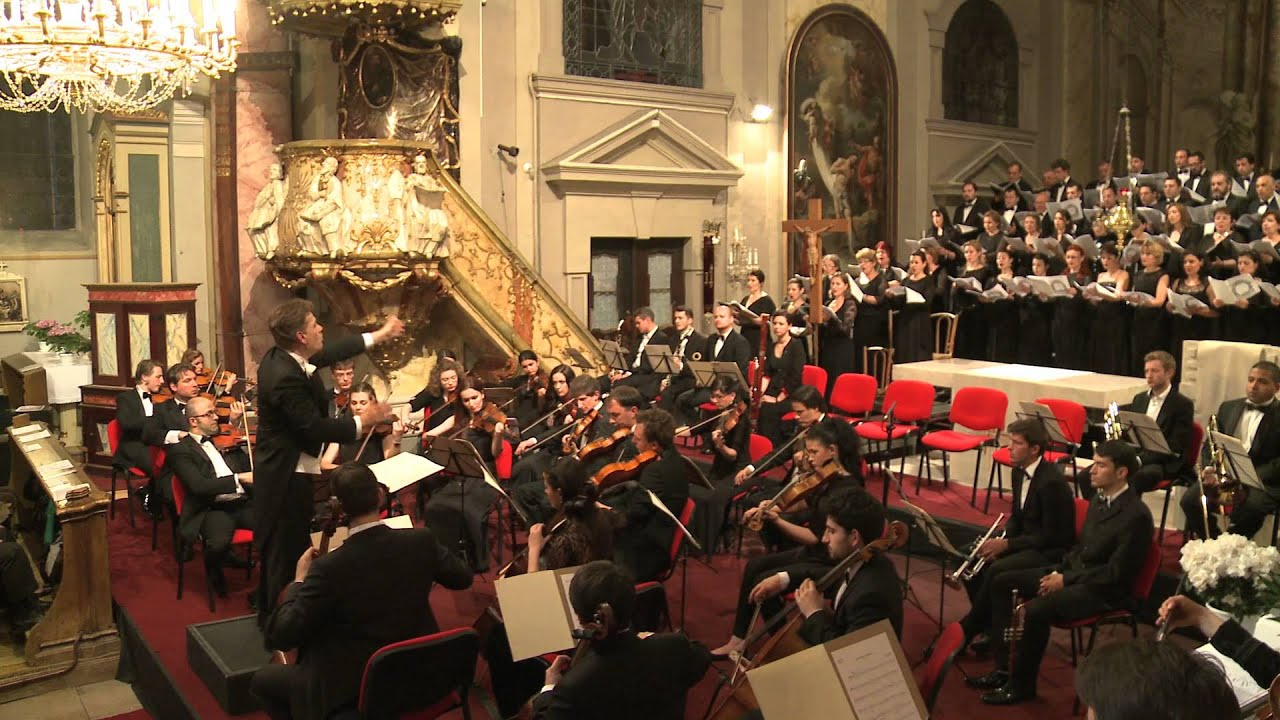
\includegraphics[width=0.48\linewidth]{pictures/youtube/2024/08/20240827_231610_youtube_001_gDKCK_6WLTg.jpg}
}
\end{center}

\subsection*{2024年08月28日 00:27}
\addcontentsline{toc}{subsection}{2024年08月28日 00:27}

\paragraph{リンク}
\url{https://youtu.be/2A7uHLyzqUY}

\begin{center}
\href{https://youtu.be/2A7uHLyzqUY}{
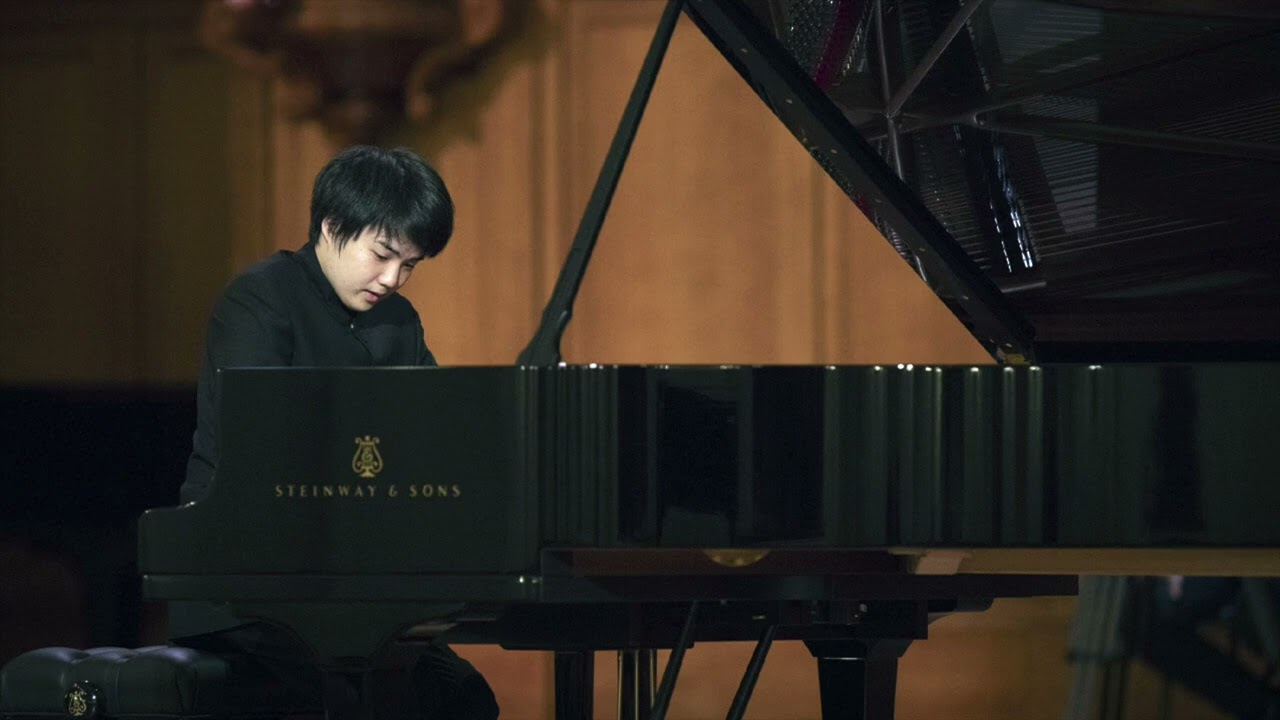
\includegraphics[width=0.48\linewidth]{pictures/youtube/2024/08/20240828_002725_youtube_001_2A7uHLyzqUY.jpg}
}
\end{center}

\subsection*{2024年08月28日 17:42}
\addcontentsline{toc}{subsection}{2024年08月28日 17:42}

\#石川県立図書館 が移転したのは2022年7月、\#金沢美術工芸大学 が移転したのが2023年10月だということです。今では、図書館と美術工芸大学の間を道路が貫いて旭坂につながり、坂を下りると田上、杜の里、\#金沢大学 の角間キャンパスにまで至ることのできる便利な道が通っています。


さて、2024年8月の現在なのですが、Google mapを見ると、県立図書館も金沢美大もまだ写っていません。その代わりに、何と、元その場所にあった \#金沢大学工学部 の建屋を撤去した跡地が写っていて、貫通道路が上から書き込まれています。今の姿は（新しい写真だったならば）道路の右側に金沢美大、左側に県立図書館があるはずなんですね。


現在の県立図書館に行こうとして、工学部の門のあった辺りに立つと、風景は全く変わってしまっているのに（奇妙なことに）昔の工学部があった頃の雰囲気を感じ（思い出し）ます。門を入るとロータリーになっていたんですね（航空写真にはそんな模様が見えています）また、各科の建屋に至る通路がはっきり写っています。この辺りに電気科の建屋、この辺りは精密の建屋、後ろには化工の建屋があったかな。正面は食堂で、その後ろには機械科だったか。入って右手（今は金沢美大）には、計算機センターがあって、そこへカードの箱を抱えて通っていました。この航空写真を見ていて、そんな夏の日、特に計算機センターの窓の外の夕方の日差し、カードにパンチ穴を空けて（入力して）いた時、ラインプリンタから計算結果が出てくるのを待っていた時、ナドナドを思い出しました。（歳とったな）

\paragraph{写真}
\begin{center}
\begin{minipage}{0.48\linewidth}
\centering
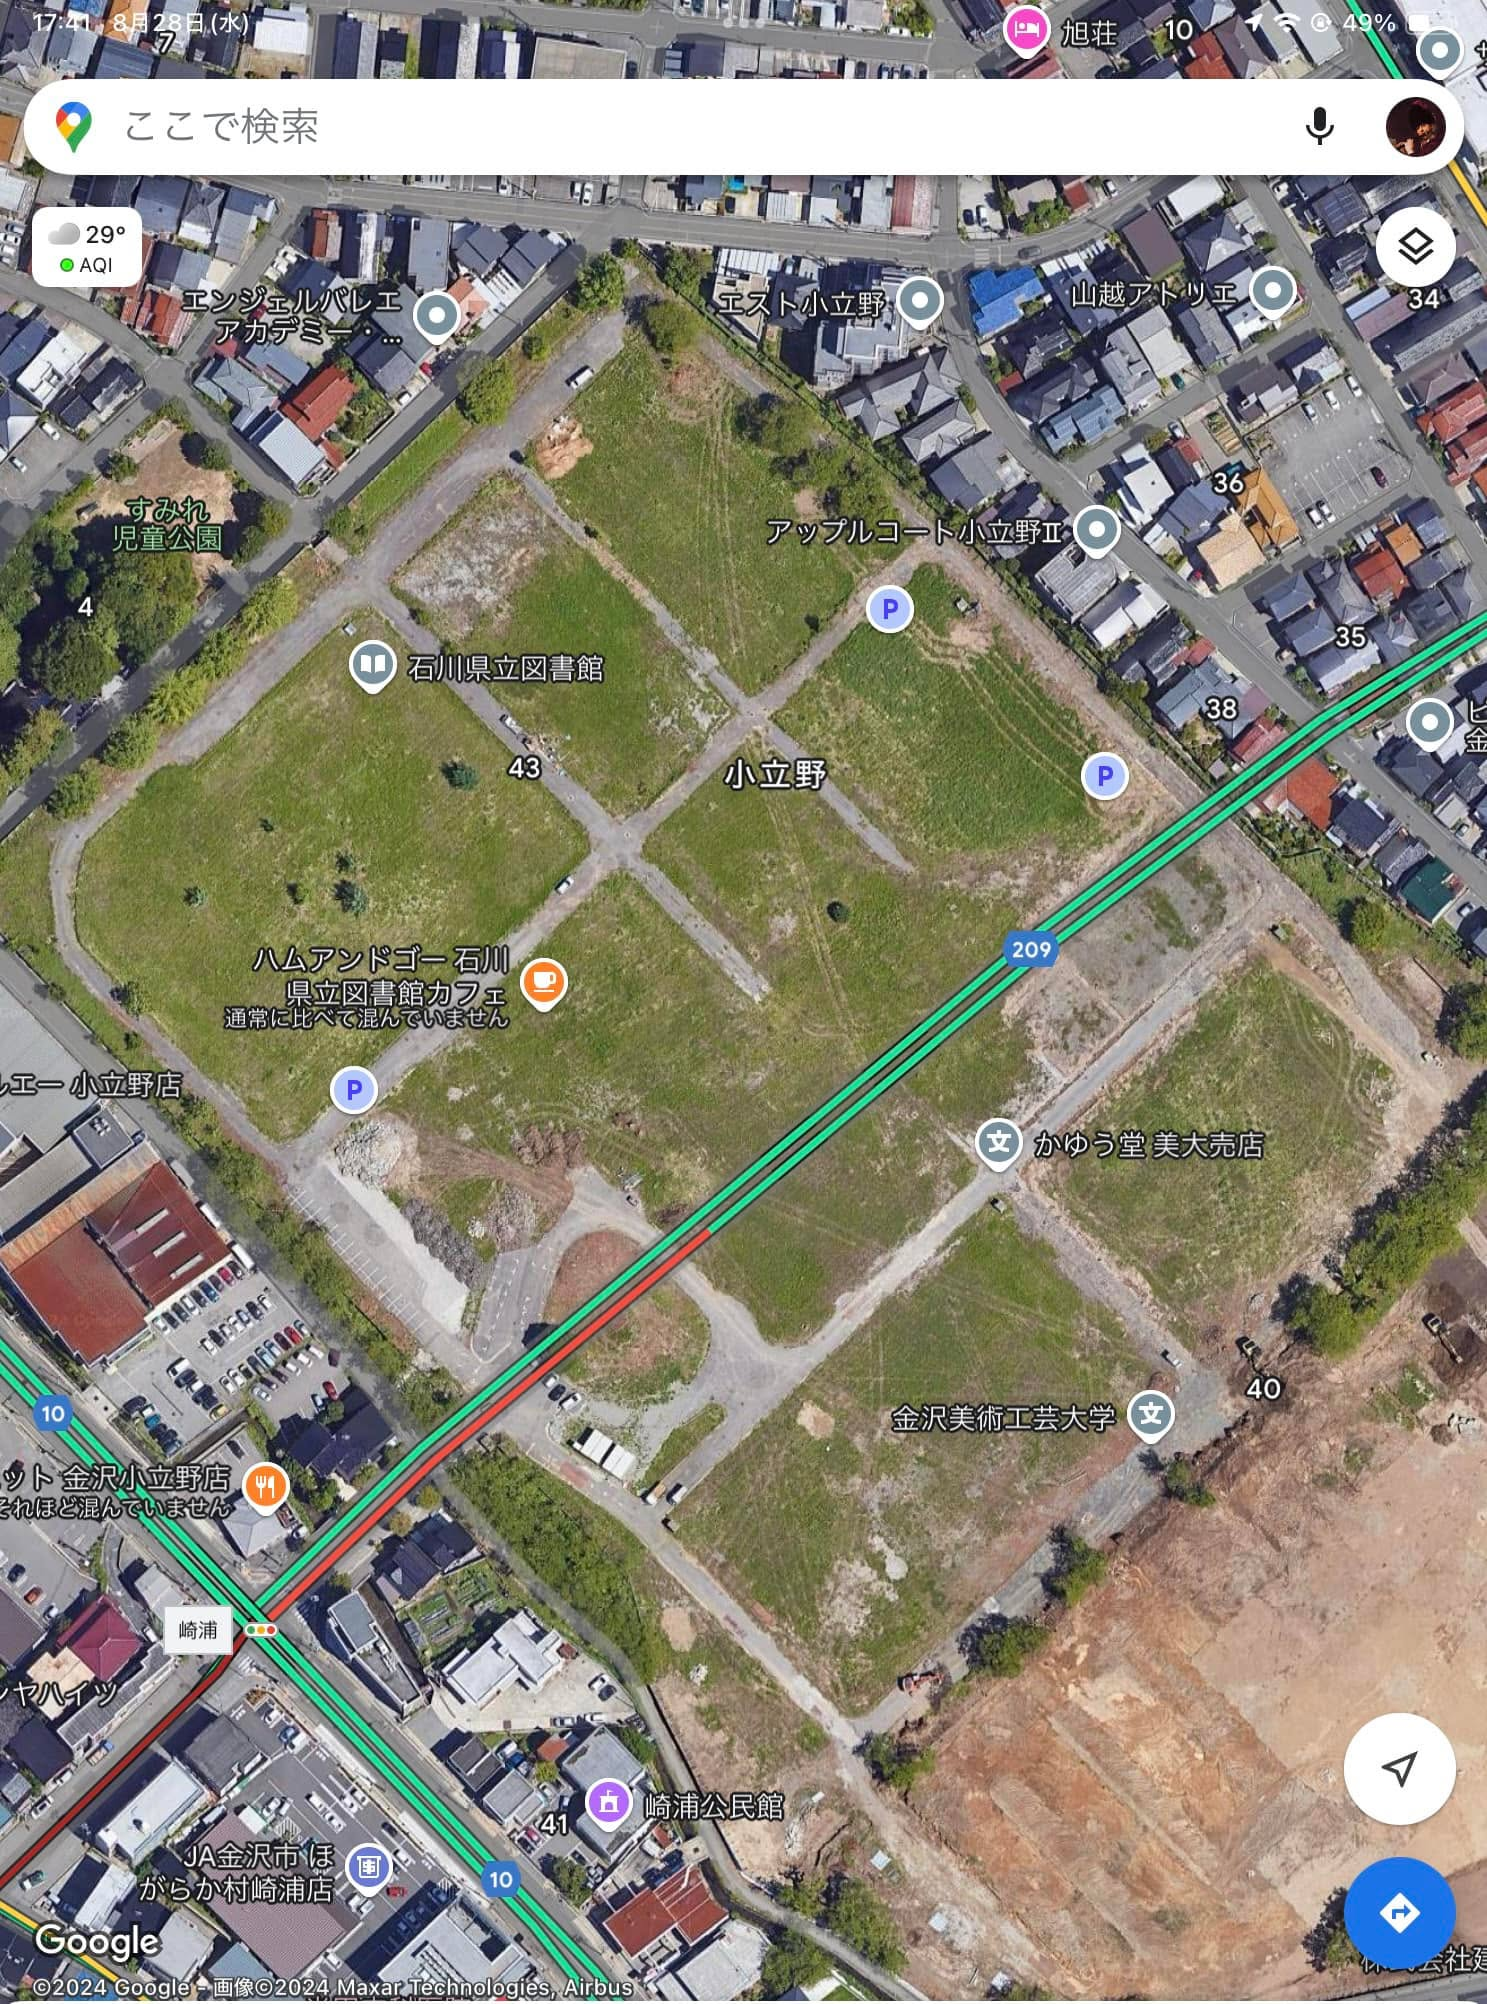
\includegraphics[width=\linewidth]{pictures/2024/08/20240828_174234_001.jpg}
\end{minipage}
\end{center}

\subsection*{2024年08月30日 00:28}
\addcontentsline{toc}{subsection}{2024年08月30日 00:28}

\paragraph{リンク}
\url{https://youtu.be/FjL3xrMgvsw}

\begin{center}
\href{https://youtu.be/FjL3xrMgvsw}{
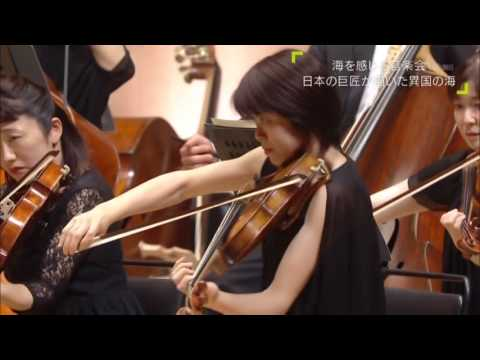
\includegraphics[width=0.48\linewidth]{pictures/youtube/2024/08/20240830_002834_youtube_001_FjL3xrMgvsw.jpg}
}
\end{center}

\subsection*{2024年08月31日 17:03}
\addcontentsline{toc}{subsection}{2024年08月31日 17:03}

\#全国学生大茶会2024 (\#学茶金沢)の第⑤会場に参加してきた。


会場の \#松声庵 は樹々の緑も雨で濡れて苔生す庭とともにとても落ち着いた佇まい。正客は「1780年創業 金沢漆器」の能作の方だった様で、松声庵の事や掛け軸の事、茶道具のことなど色々とお話しくださり、とても興味深く伺いました。

また、\#平安女学院大学 の学生さんたちも、綺麗な着物を着てもてなして下さり、そしてベトナムやらカンボジアやらフランスやらの茶碗でお茶をいれて下さいました。さすが \#国際観光学部 の皆さんですね。大学の講義でもこうしたお茶などの日本文化も学ばれているとのことでした。（指導されている先生がまた素晴らしい（厳しい）方なんだと正客さんが話していらっしゃいました）

平安女学院大学さんは昨年度もこのイベントに応募されたそうですが、抽選でもれてしまい参加できなかったそうです。（一昨年は参加されていたとか）会場の数が限られているせいでしょうか。素晴らしいお手前を次回もまた披露して頂けると嬉しいことです。


正直なところ、この様なお茶会は初めてだったので、少々緊張しました。（ひたすら前の人の真似をしていましたよ）

\paragraph{写真}
\begin{center}
\begin{minipage}{0.48\linewidth}
\centering
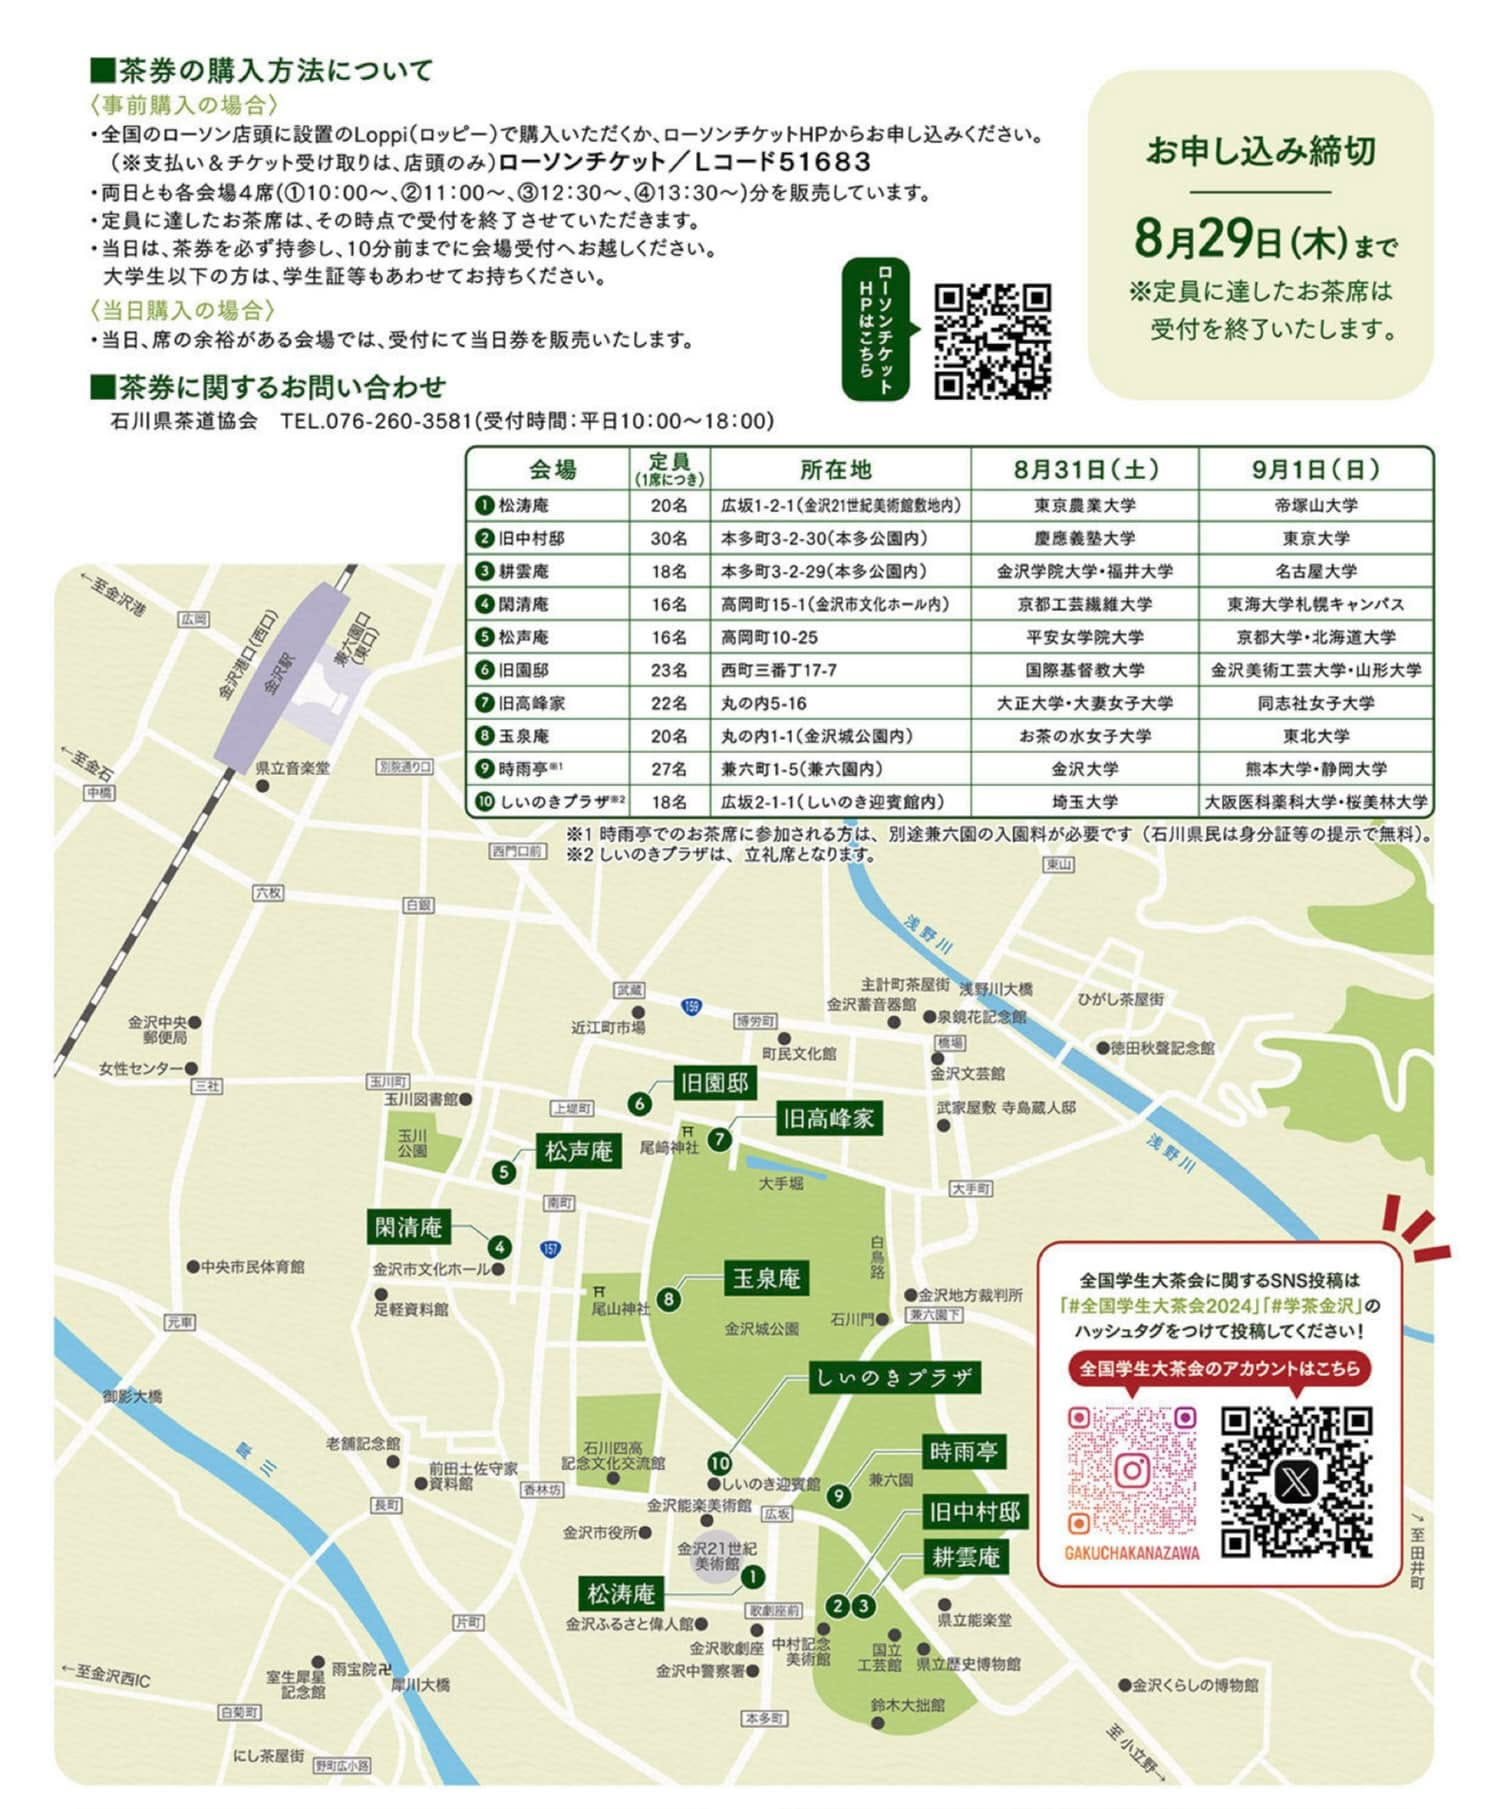
\includegraphics[width=\linewidth]{pictures/2024/08/20240831_170358_001.jpg}
\end{minipage}
\hfill
\begin{minipage}{0.48\linewidth}
\centering
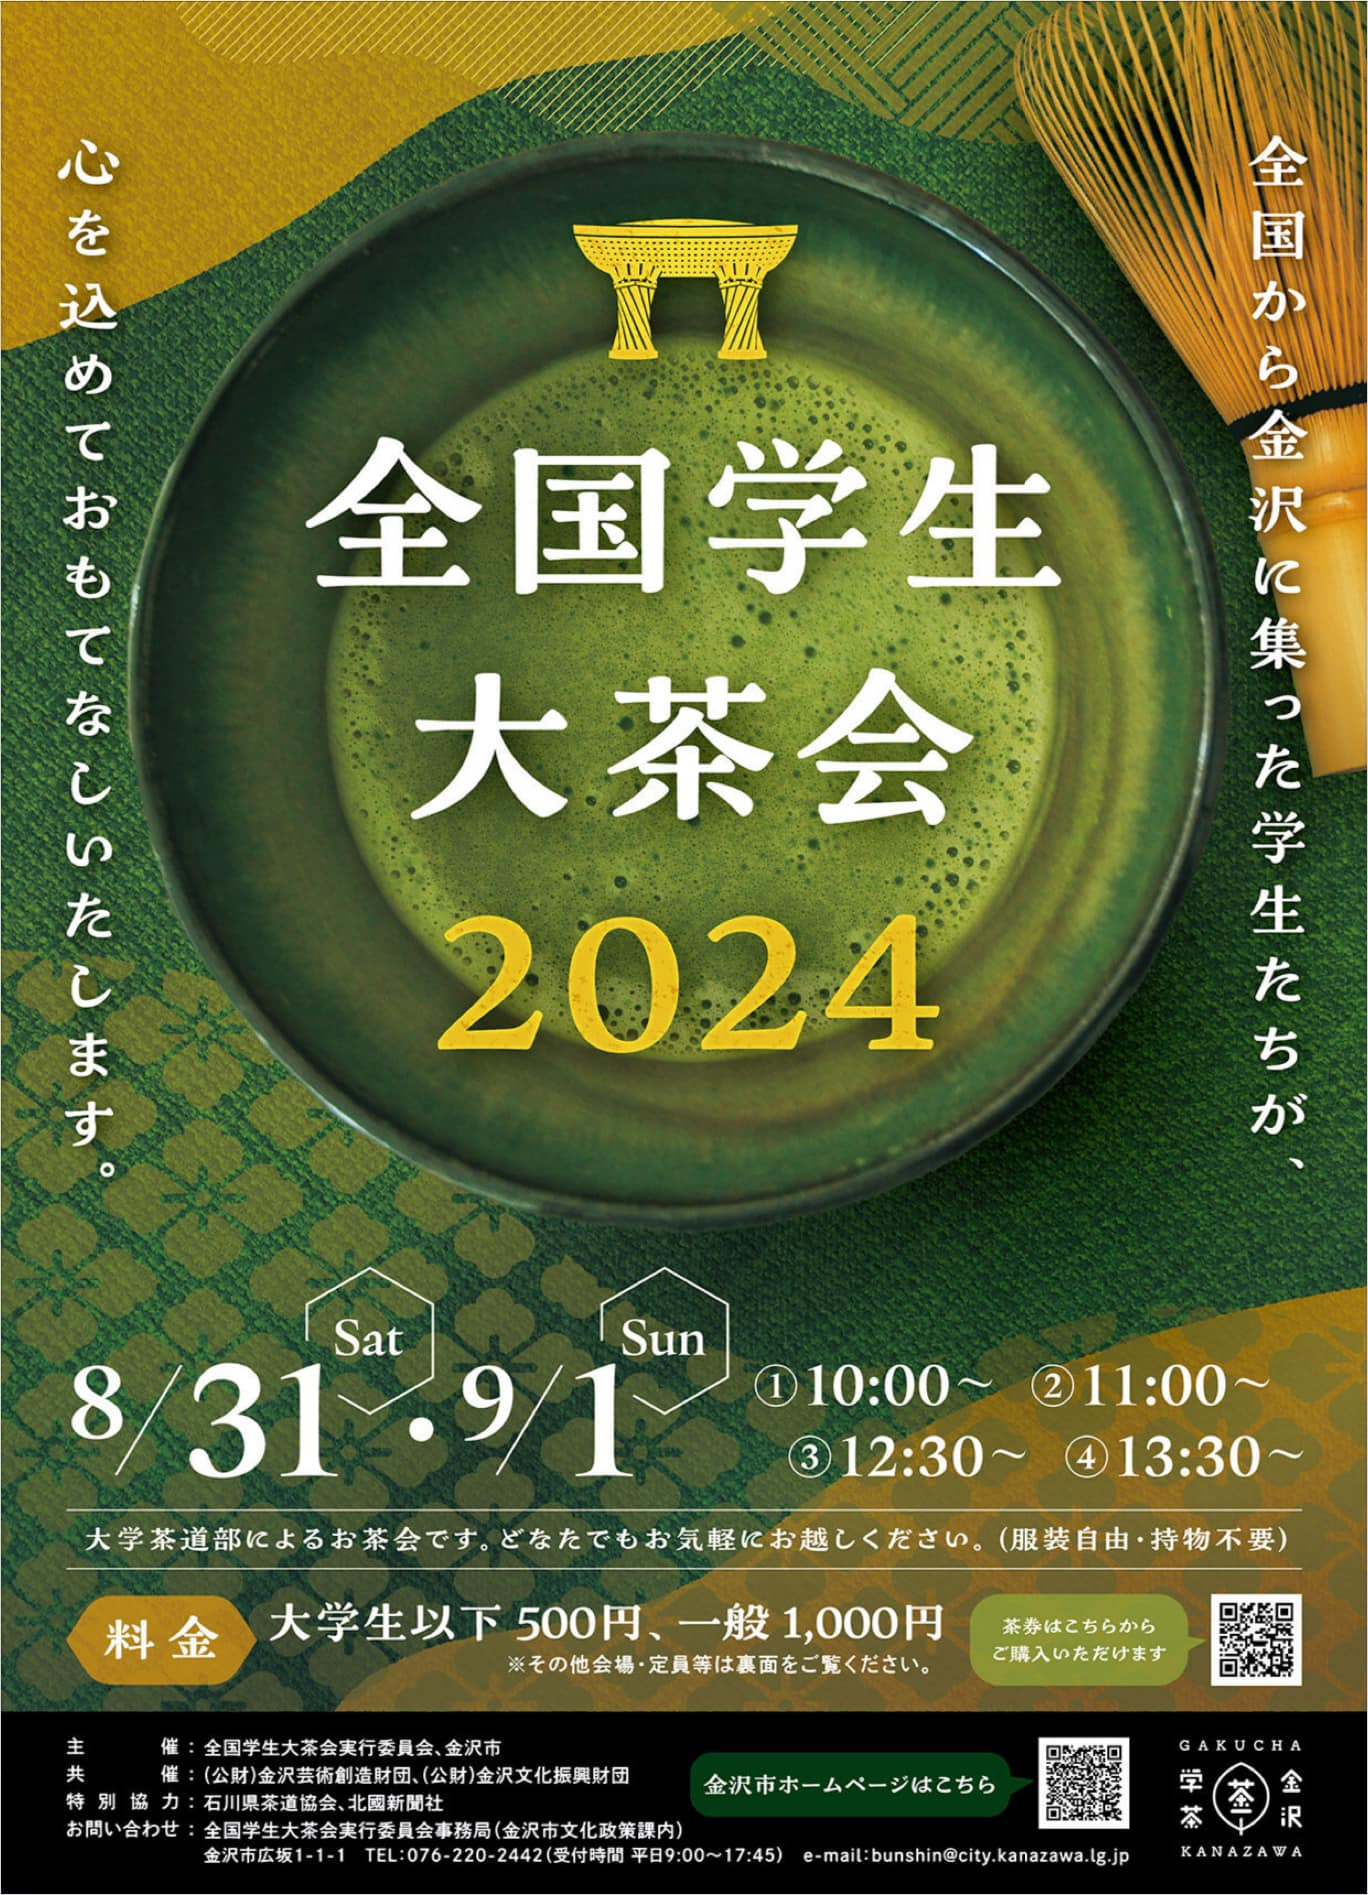
\includegraphics[width=\linewidth]{pictures/2024/08/20240831_170358_002.jpg}
\end{minipage}
\end{center}

\section{9月}

\subsection*{2024年09月03日 09:00}
\addcontentsline{toc}{subsection}{2024年09月03日 09:00}

\paragraph{リンク}
\url{https://youtu.be/9aHo3kkgmLs}

\begin{center}
\href{https://youtu.be/9aHo3kkgmLs}{
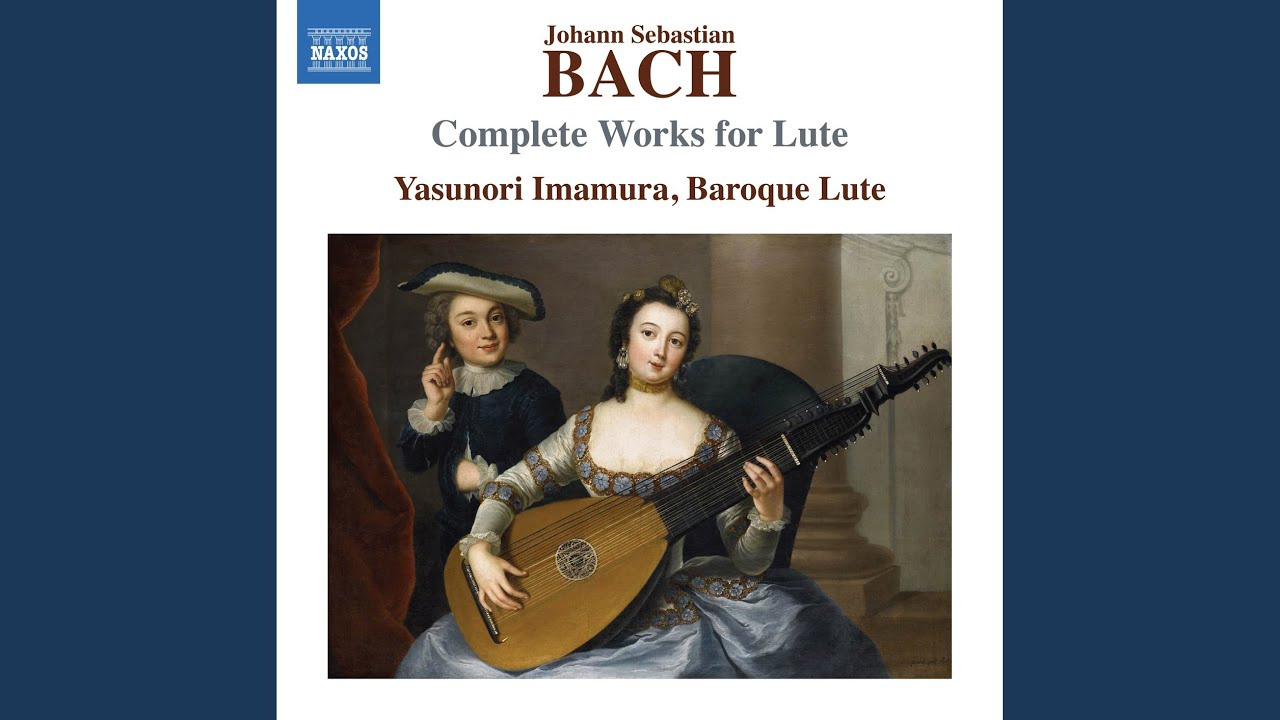
\includegraphics[width=0.48\linewidth]{pictures/youtube/2024/09/20240903_090020_youtube_001_9aHo3kkgmLs.jpg}
}
\end{center}

\subsection*{2024年09月07日 06:40}
\addcontentsline{toc}{subsection}{2024年09月07日 06:40}

\url{https://m.facebook.com/groups/771018526696066/permalink/1942960002835240/}




ここのグループを時々覗くことがある。


「運動の第二法則を証明せよ」と言うスレに対するコメントを見ていたところ、「これは法則なので証明できません」とか「自然界の法則として広く受け入れられていることだ」或いは「定義から明らかなものを命令形で問うのは失礼だ」などのコメントがあった。（クワバラクワバラ）


先ず、「法則なので。。」や「定義から明らか」などで一括してしまうのは、物理の愛好家らしからぬ所業？と言わざるを得ません。私個人としては、確かに「証明せよ」には違和感がありましたが（問の答えにはなっていないかもしれないけど）あれこれ考え、思いを巡らせたことがありました。直接コメントするのは怖い？ので、ここで独り言を言うことにしようと思います。


一つ目に思ったことは、「力が加わっていないと等速直線運動する」と言う高校物理の入り口で聞く台詞です。あの時「何で直線運動なんだろう」とか「何で等速なんだろう」と疑問に思ったまま時間が過ぎて行った事を思い出しました。

後にファインマンの力学を斜め読みしていた時に「なるほど」と印象に残った箇所がありました。それは「向きを変えたり加速減速させようとするなら、何らかの力が必要になる」という記述です。つまり、右に向かわせたいなら右へ引っ張らなくちゃいけないとか、加速させたいなら押してやらなきゃいけないという、本当に普通のことを言っていたんですね。逆を考えると、力が加わってないなら、向きも変わらないし加速減速もしない、つまり等速直線運動しているという事になります。お月さんも国際宇宙ステーションも、地球に向けて引っ張る力をかけ続けなかったら、真っ直ぐ直線運動で宇宙の彼方へ飛んで行ってしまうものなんですよね。


実はこの事は、第二法則の式に書かれている事を言葉で言っているのと同じです。つまり「力が加わっていない、即ちF＝0」の場合、運動方程式を見ると、（質量mは定数>0）の下で dv/dt=0とならざるを得ず、微分してゼロという事は「vは定数」だという事、つまり等速運動だと言っている事になります。さらにベクトル量としての力の向きは（加）速度の向きと平行（大きさはスカラm倍）だと第二法則の式は言っています。そんな訳で運動の第二法則の式は「力が加わっていないと等速直線運動する」となるのでした。（じゃあ慣性の法則はどうなる？）


二つ目に思ったことは、いわゆる解析力学で導入される変分原理をスタート点に認めることにすれば、ラグランジアンL=T−Uに対するEular-Lagrange equation から、第二法則の運動方程式を導き出せたという事です。変分原理（最小作用の原理とかHamiltonの原理とかとの区別についての理解は曖昧なんだけど）を黙って認める事が必要だという意味では、単に問題を置き換えたに過ぎないという事なのでしょうか？（Hamiltonianでもニュートンを定式化してましたよね）

\subsection*{2024年09月12日 09:34}
\addcontentsline{toc}{subsection}{2024年09月12日 09:34}

応援中: Lucie Horsch ―ライジングファンに認定されました！🎉

\paragraph{写真}
\begin{center}
\begin{minipage}{0.48\linewidth}
\centering
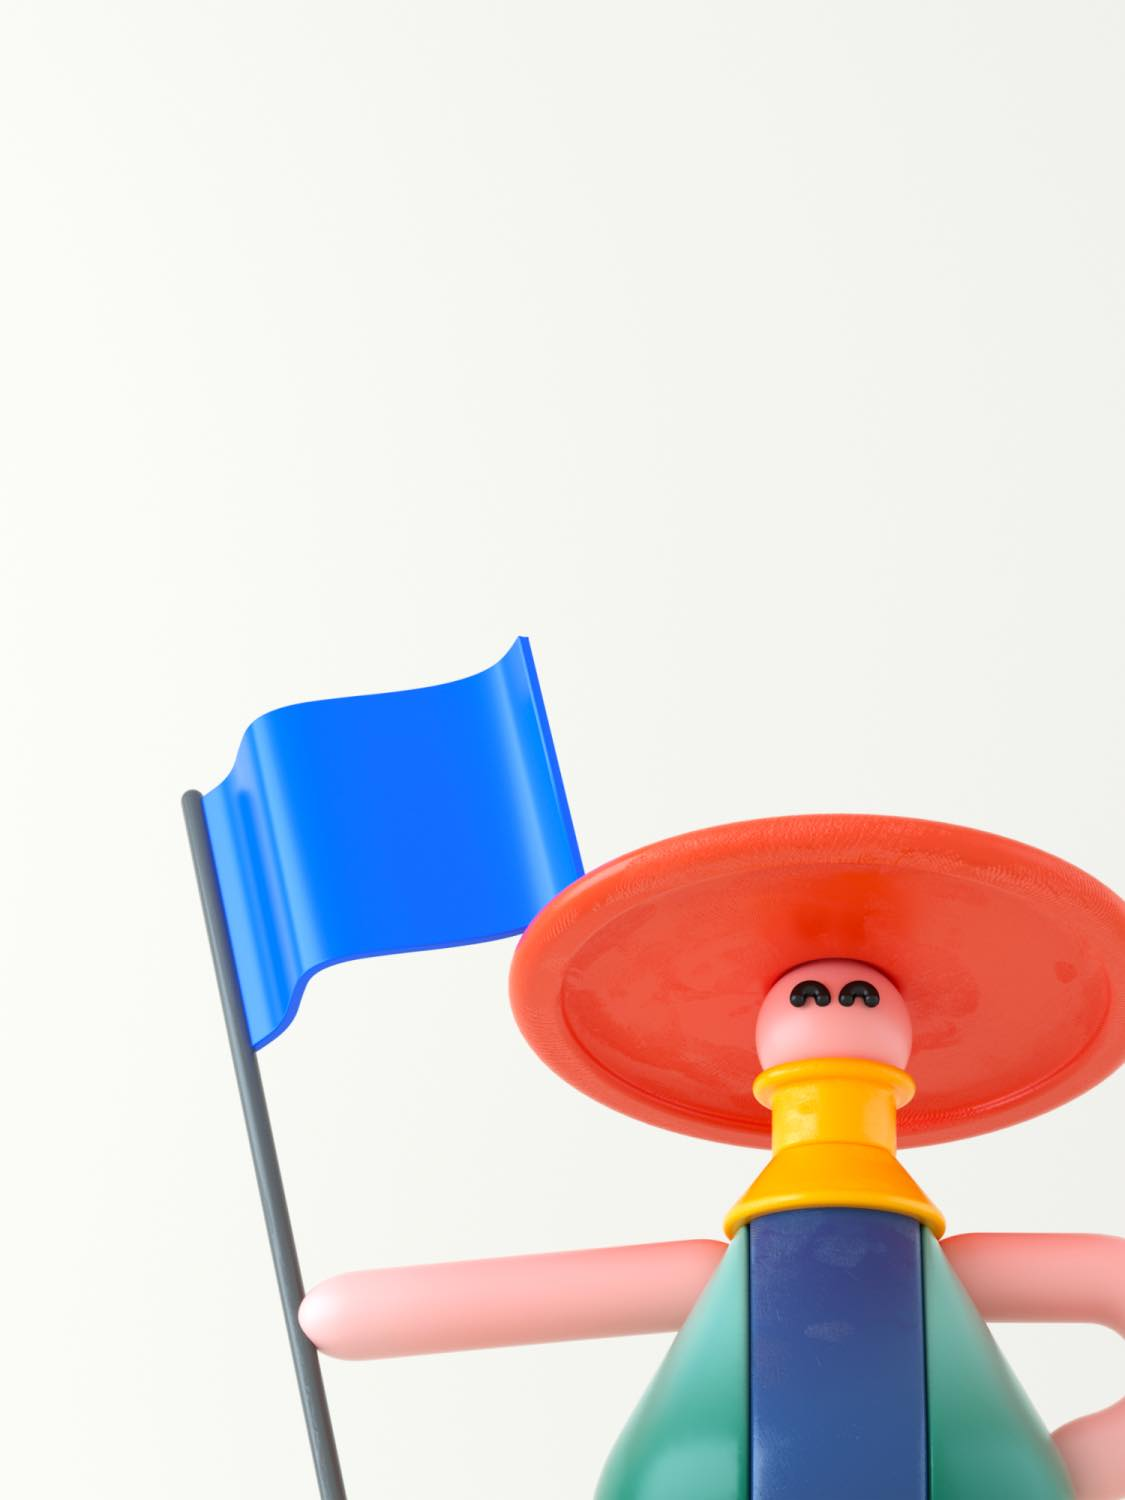
\includegraphics[width=\linewidth]{pictures/2024/09/20240912_093447_001.jpg}
\end{minipage}
\end{center}

\subsection*{2024年09月12日 11:00}
\addcontentsline{toc}{subsection}{2024年09月12日 11:00}

以前から津波対策について思っていることがある。


ノイズキャンセリングに対応したイヤフォンやヘッドフォンが普及している。その原理はつまり、マイクで取り込んだノイズの波形の位相を反転させた波形（音）をスピーカから発して、ノイズと合成された波形が平坦になる事を狙っている（のでしょう、おそらく）。


一方で、大掛かりなプールなどで波を発生させたり、サーフィン用のビッグwaveを発生させたりする事は、ある程度出来るようです。あとは発生させる波の位相や波長を思い通り制御する必要はあると思いますし、発生させる波の規模（振幅）も、現状では津波に比べて全く非力なのかもしれません。


気を取り直して、「津波に対してノイズキャンセリングと同様の仕組み」は出来ないものでしょうか。


(１)イヤホンのマイクの音を解析するよりも、ずっと時間的な余裕のあるケースが多いような気がする

(２)完全に波高を潰せなくても、多少低く出来る可能性はないのか

(３)津波そのものと同規模の波を作って対向させるエネルギは大きすぎる。あり得ない。しかし小規模の波で、複数回の対策波を複数箇所から連続して（時間間隔=>位相をコントロールして）発射して波高を抑えていく事はできそうな気がする

(４)津波の対策波を複数発射させる場合、全体として制御された動作にしないと、逆に余計な波を作ってしまったり、逆に誤って位相が合ってしまうと振幅が足し算になってしまう可能性があるので要注意だ

(５)防波堤を静的な受身の防波堤ではなくて、動的な動きが可能な防波堤にできると、もっと色々対策できるんじゃないのかなぁ。そもそも津波到着時に、防波堤の位置を津波の波長の1／4の距離だけ移動させたらどうなる？津波到着時にそのタイミングで振幅分だけ水面（防波堤に沿った海底）を下げたらどうなる？（防波堤に可動部分を作ったりなんかしてたら、あっという間に壊れちゃうかも）


誰か既に研究している人いるのかな？土木工学あたりで。

\subsection*{2024年09月13日 05:58}
\addcontentsline{toc}{subsection}{2024年09月13日 05:58}

疑問に感じていた事なのですが、解析力学に出てくる次の様な（なんとなく重要そうな）「原理」の数々、(１)変分原理、(２)最小作用の原理、(３)Hamiltonの原理、(４)仮想仕事の原理、まだ何かありましたっけ？ダランベール？未定乗数法？そうだ（５）極小原理、なんてのもあった様な気がします。


そもそも、これらの間の違いとはいったい何なんでしょう？それぞれの項にある式を追いかけたり例題を解いたりするのに精一杯で、俯瞰的に見えていませんでした。正直に言うと、「どれも似た様なことを言っている」様な気がしてなりません。それなのに、それら似た様な「原理」なるものが「次から次へ」と現れてくるので、頭の中は全くもって整理できていないのです。できれば(１)「だけ」で一括して（統一して）欲しいくらいです。（少なくとも(２)と(３)はどうも同じ事柄を指しているらしいし、それだけで十分らしい）


解析力学で勉強した事は、LagrangianによってもHamiltonianによっても古典的なニュートン力学を記述できるよって事でした。それらの基礎となる理論的背景として変分法（の類い）があるよ「という感じ」だったと思います。いずれ解析力学の全体を俯瞰して、この「もやもや」をハッキリさせたいものです。

\subsection*{2024年09月16日 00:48}
\addcontentsline{toc}{subsection}{2024年09月16日 00:48}

\url{https://m.facebook.com/story.php?story_fbid=1205638727170693&id=100031737316033}




第３回を聴講した。

長かった〜。19時開始で終わったのは22時を過ぎていた？各章の区切りで休憩にすればいいのにと思ったりしました。講師の前田りり子氏は（録画とは言え）本当に元気な方なんだな。録画が終了した後にはzoomで質疑応答ですから。


（１）アポジャツーラ（ローマ字打ちでtu はツになってしまう）のルールが初耳だった。

（２）フリードリヒ大王の時代に、大バッハは既に過去の人になっていたんですね。モーツァルト的音楽に既に向かおうとしていた。そう言えば、大バッハの息子の曲、エマニュエルではなくて誰でしたっけ、モーツァルトっぽい曲だったのを聞いたことがあります。

（３）大バッハは対位法的な曲を書いてきたけど、だんだんモーツァルト的な音楽（旋律と伴奏）が好まれる時代になりつつあった。大バッハが書いて献呈した「音楽の捧げ物」ですけど、フリードリヒ大王もクヴァンツも開いて見る事はなかったし演奏する事もなかった（かもしれない）と聞いてショックでした。また、「王のテーマ」も以前クヴァンツが何処かで書いていたものかも？と言うのも、何だか年寄りの大バッハを小馬鹿にした様な当時の雰囲気が感じられて悲しくなるな。

（４）前打音に長い（8分音符）ものと短い（16分音符）ものがあって、演奏法の違いがよく分かりました。大バッハのフルートソナタの例がわかりやすかった。

(５)ヘンデルのフルートソナタのゆっくりの楽章（例えばe-moll HWV359bの３楽章Adagio）で、複雑な装飾を施して演奏されているのを聞いたことがある。楽譜はとってもシンプルなのに、こんなに複雑な装飾を施されたら、その通り（超シンプルな楽譜の通り）に吹く気にはとてもなれませんよ。当時の作曲家は曲の骨格だけを楽譜にして、基本的に演奏者が装飾を付けて演奏していた。（大バッハのゆっくりした楽章でもいろいろ装飾付けた演奏ありますもんね。例えばチェロ組曲六番のSarabande など）

(６)クープランは楽譜に装飾を力一杯書いていた。作曲者の性格か？

(７)トリルは上からと信じていたけど、下からの場合もあったのか。


＃前田りり子 \#トラヴェルソ \#Quantz \#クヴァンツ \#フルート奏法


⚪︎第一回目の聴講

\url{https://m.facebook.com/story.php?story_fbid=7876849065732519&id=100002225117991}




⚪︎第二回目の聴講

\url{https://m.facebook.com/story.php?story_fbid=1182866802781219&id=100031737316033}



\subsection*{2024年09月22日 19:49}
\addcontentsline{toc}{subsection}{2024年09月22日 19:49}

\#金沢城 の石垣の石ですが、

①\#戸室山（現金沢大学の裏辺りの山か？）から \#戸室石 を切出し

②\#下田上橋 橋詰 辺りで、\#浅野川 に竹籠を敷いた上を戸室石を渡し

③\#野坂 を通って \#小立野台地 まで石を引き上げて

④台地上を（現石引通りを）金沢城まで曳いてきて、石垣に組み上げた

という事の様です。


今日（9/22）(雨や嵐の合間を縫って）「\#御山まつり」がありました

(１)\#金沢神社（兼六園の横にある神社）の神様が御神輿で今日一日石引界隈を巡られました

(２)石引一丁目の交差点にある下馬地蔵を起点として、\#石引通り を戸室石を曳く催しが行われました

(３)周辺の中高大学の音楽系サークルの演奏やダンスなどが披露されました


石引一丁目の \#下馬地蔵 前から、石が曳き始められるのを見ていると、「野坂」の所在の確認に出かけたくなりました。（小雨の中でしたが）

石川県立図書館と美術工芸大学の間を突っ切っている道路から旭坂を下ります。遠くに戸室山と思われる山も見えています。旭坂を降り切ると、ちょうど浅野川の下田上橋（しもたがみばし）の橋詰（はしづめ）に（三叉路の信号に）至ります。そこに「野坂」について記述された標識があります。その記述にある様に、実際の「野坂」の上り口は、その標識から旭坂を150m程登った辺りにあるとの事。行って見ると、雑草に隠れそうになっている「野坂の登り口」と書かれた標識を発見しました。深い雑草に埋もれていて、しかもかなり急そうな坂の様子でしたので、おそらくは、小立野台地まで石を持ち上げるというのは、かなり大変な事だっただろうと推察します。現在はとても人が登れる様な状態に整備されていない（蛇や熊に出会えそう）そんな坂の様相でした。

\paragraph{写真}
\begin{center}
\begin{minipage}{0.48\linewidth}
\centering
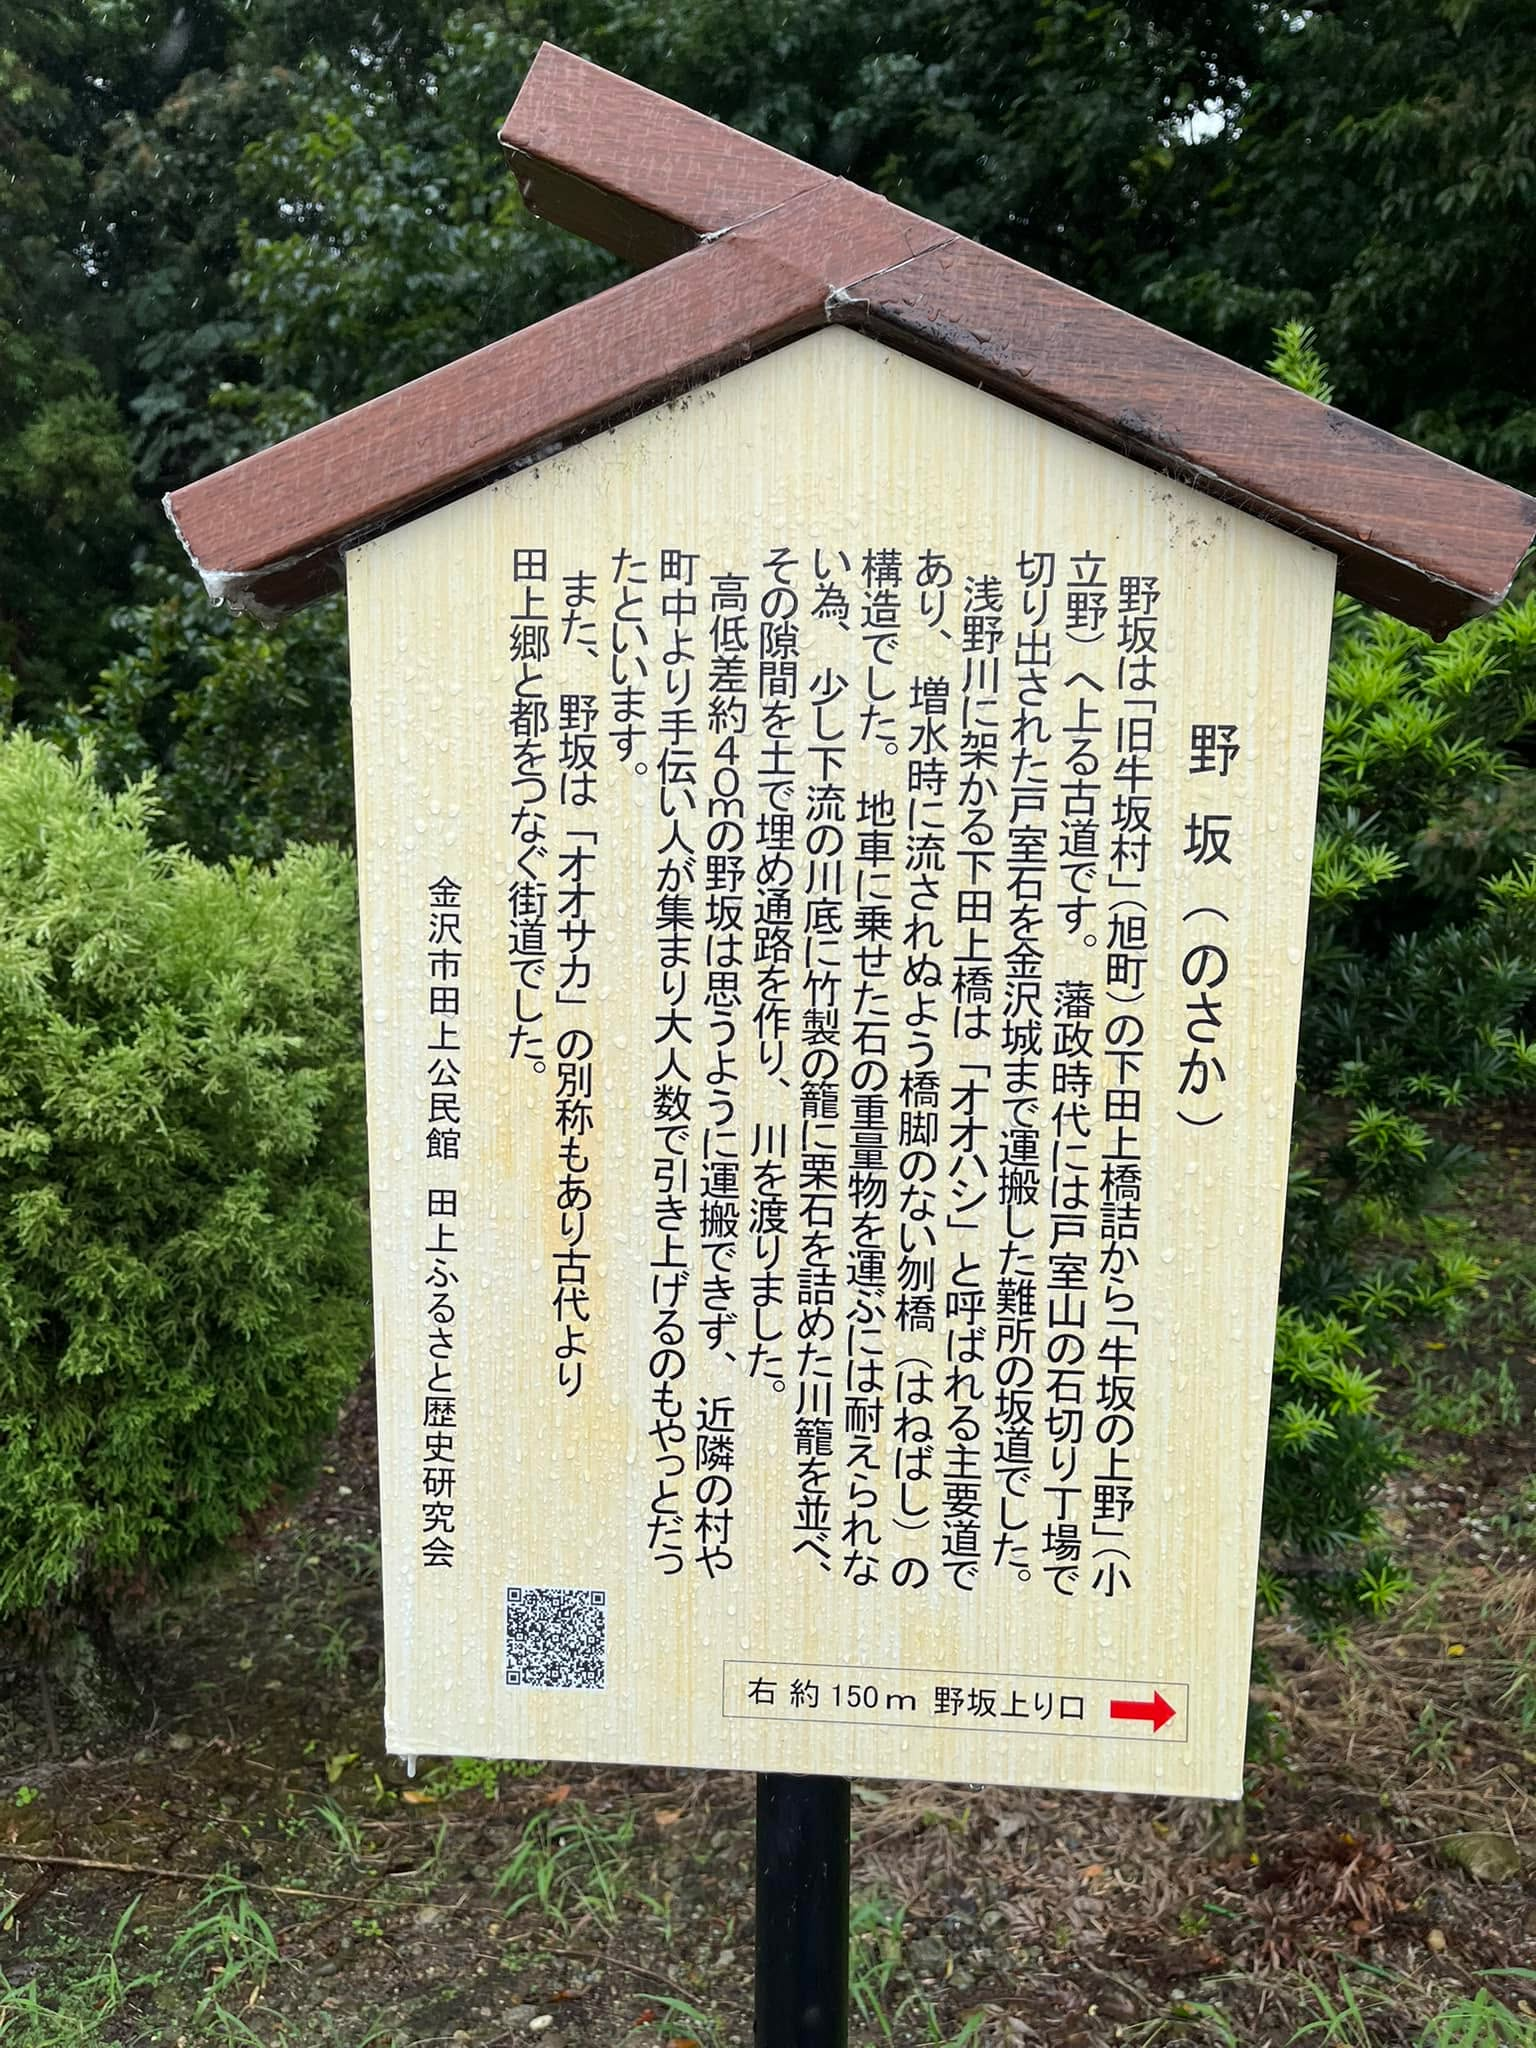
\includegraphics[width=\linewidth]{pictures/2024/09/20240922_194920_001.jpg}
\end{minipage}
\hfill
\begin{minipage}{0.48\linewidth}
\centering
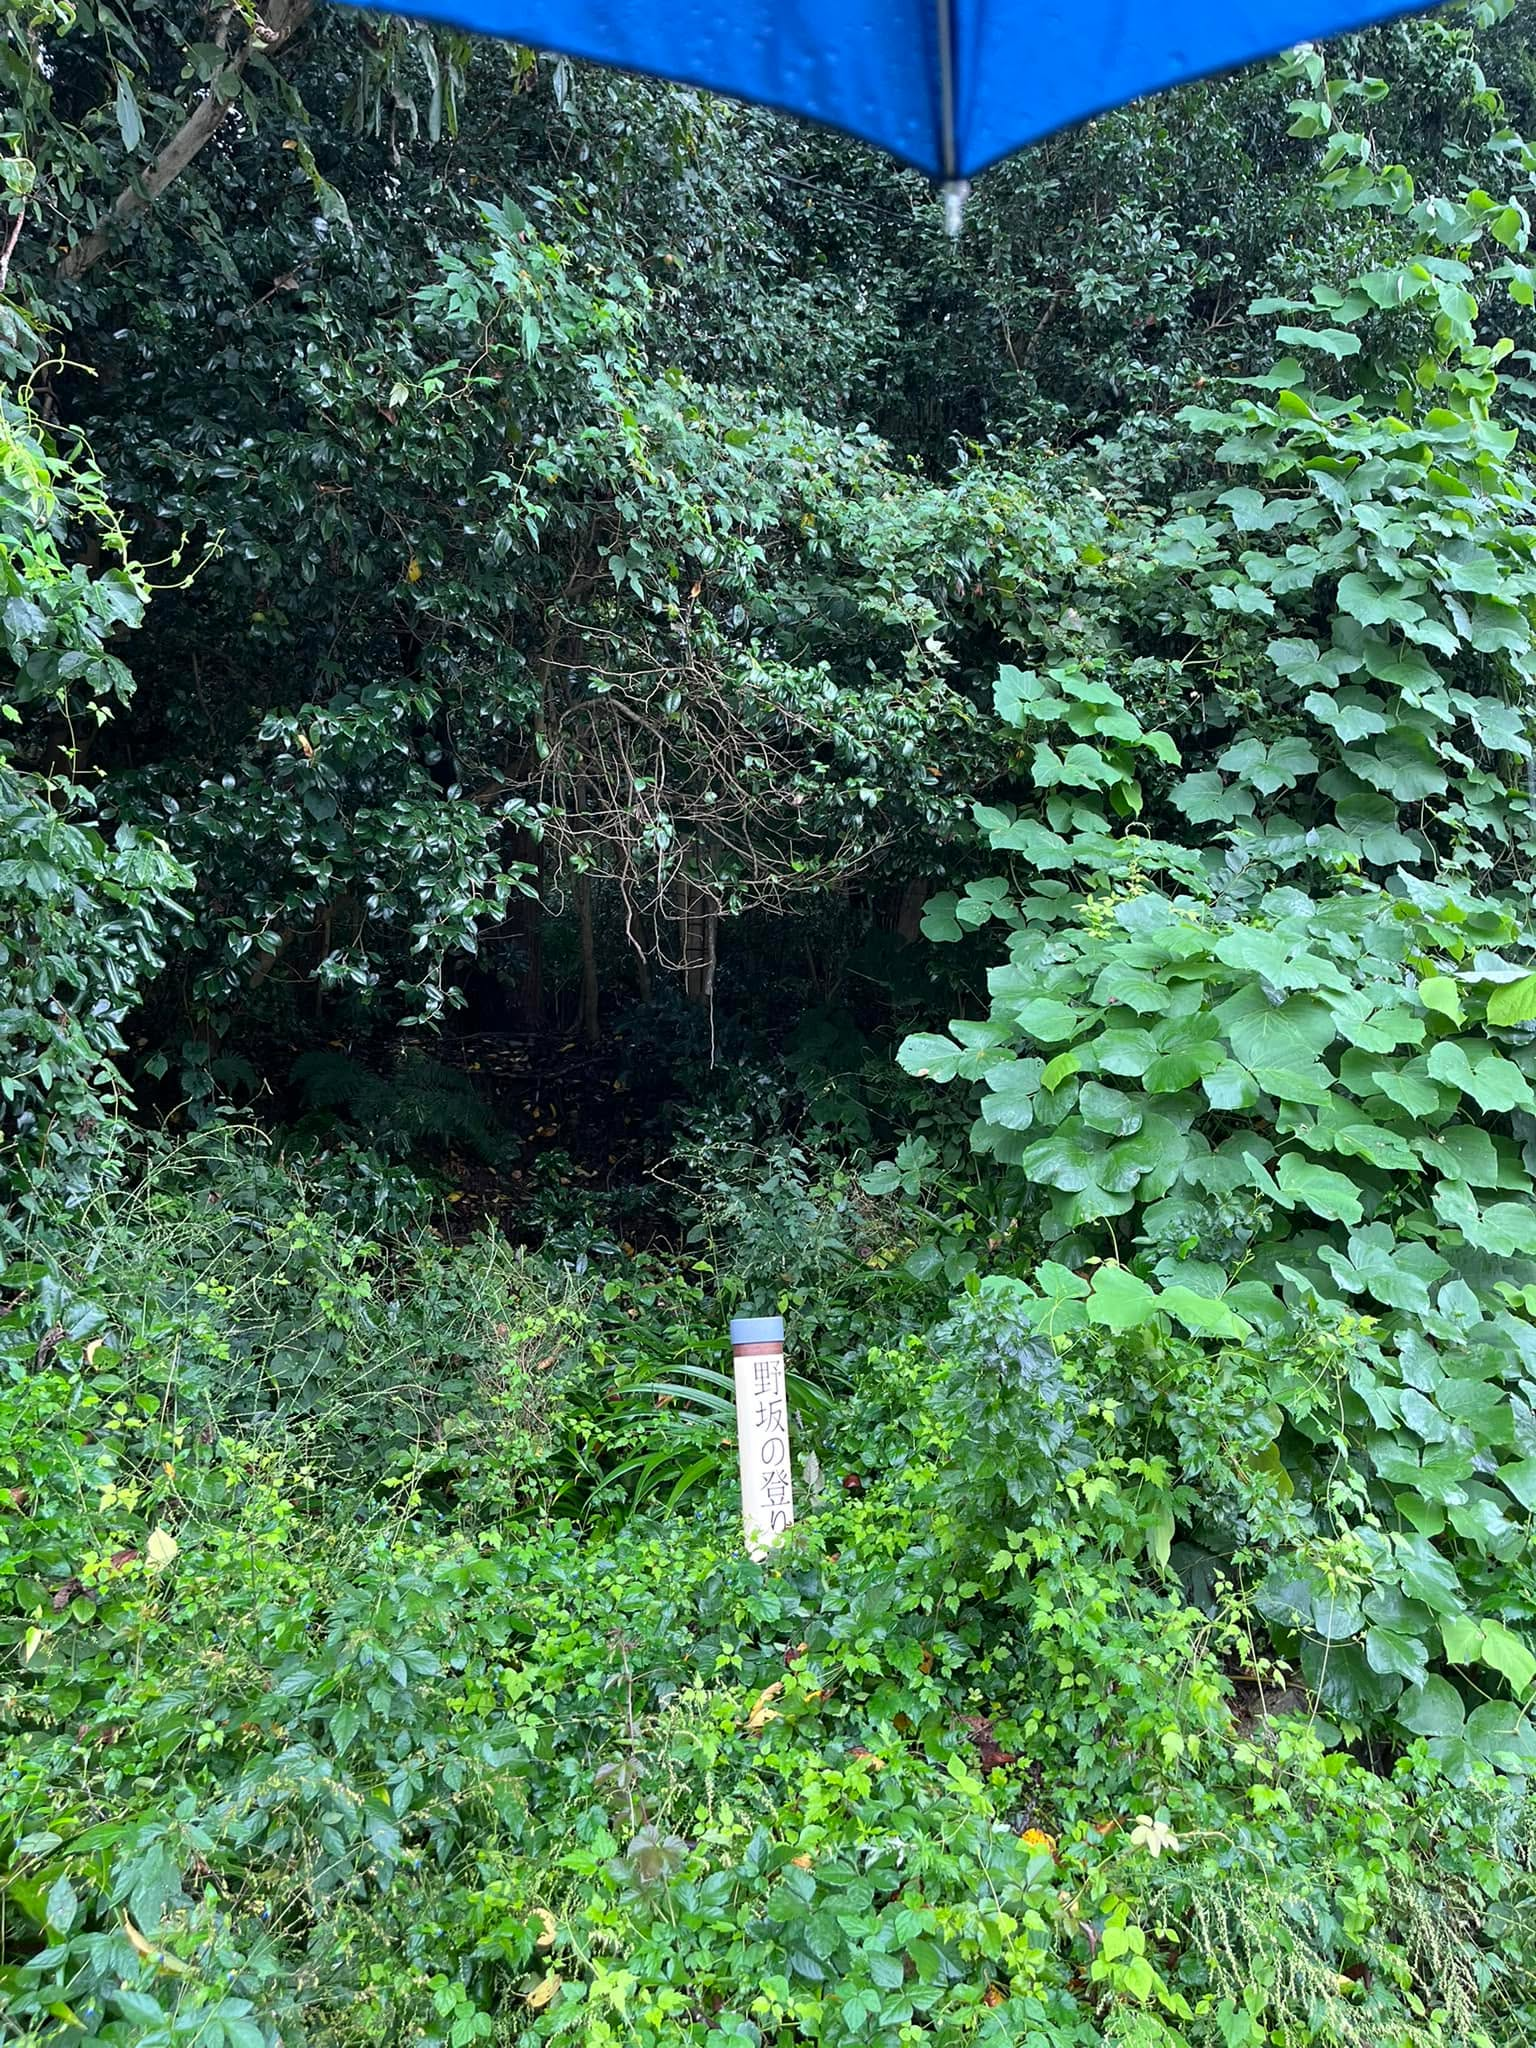
\includegraphics[width=\linewidth]{pictures/2024/09/20240922_194920_002.jpg}
\end{minipage}
\end{center}

\begin{center}
\begin{minipage}{0.48\linewidth}
\centering
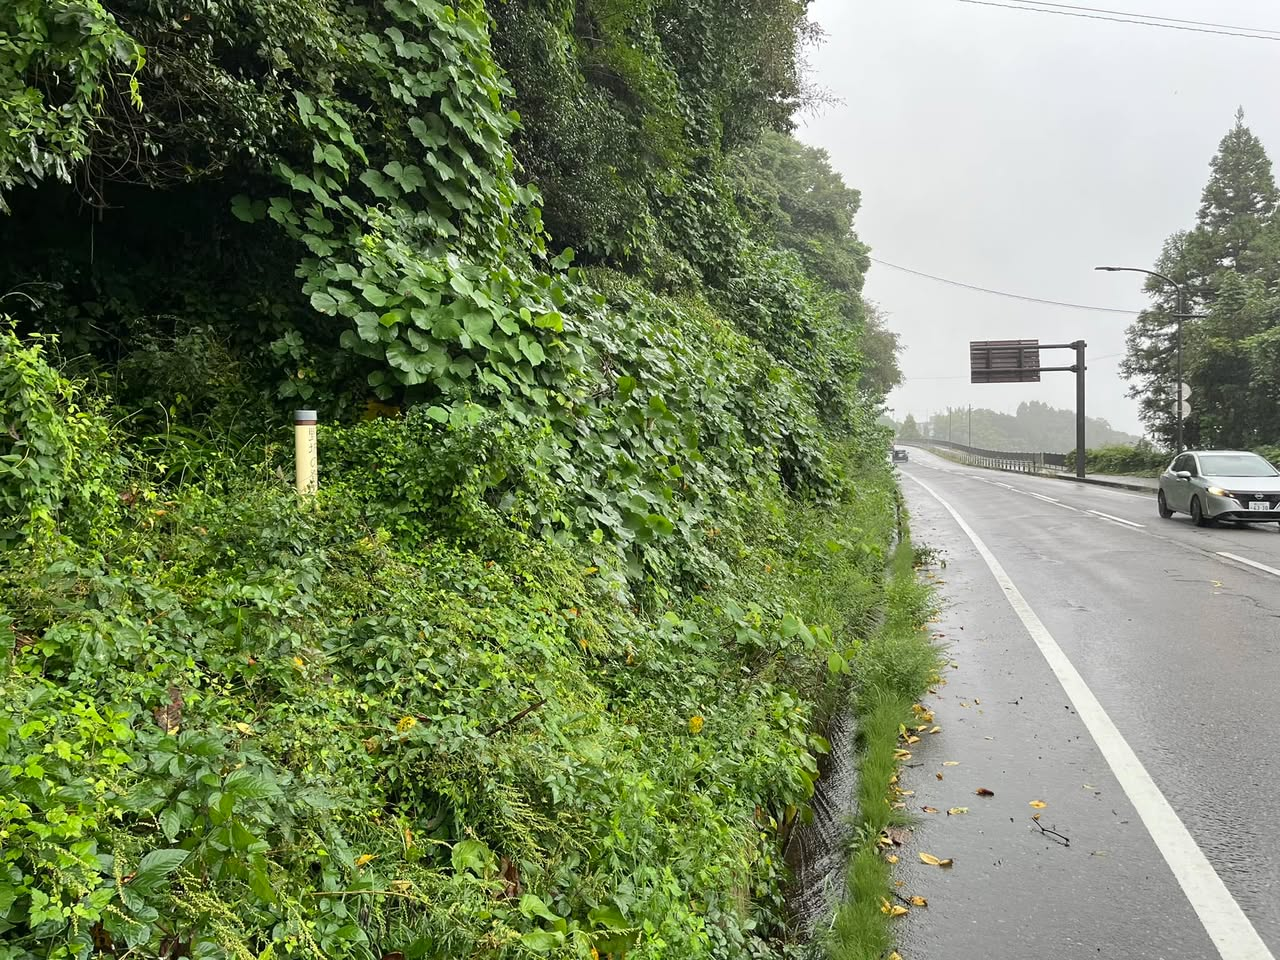
\includegraphics[width=\linewidth]{pictures/2024/09/20240922_194920_003.jpg}
\end{minipage}
\hfill
\begin{minipage}{0.48\linewidth}
\centering
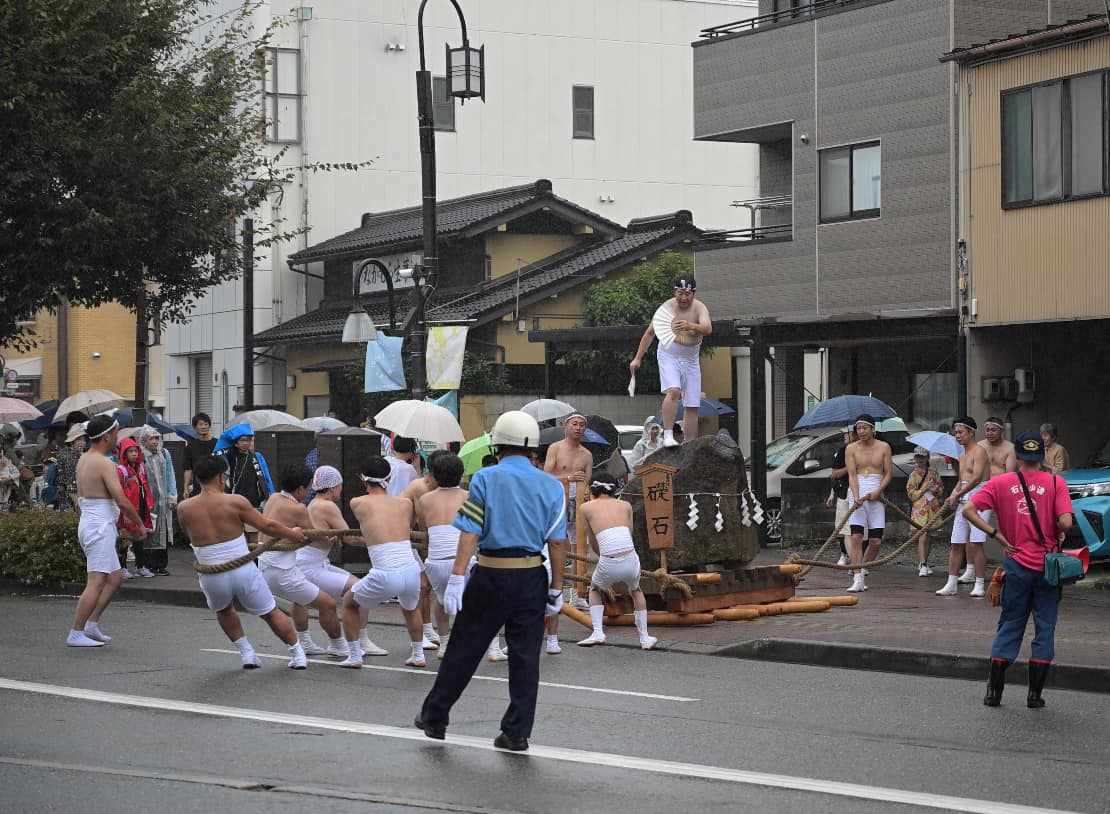
\includegraphics[width=\linewidth]{pictures/2024/09/20240922_194920_004.jpg}
\end{minipage}
\end{center}

\subsection*{2024年09月25日 13:08}
\addcontentsline{toc}{subsection}{2024年09月25日 13:08}

\url{https://fb.watch/uPhBKmYwu5/}




\url{https://fb.watch/wnab-hgKgh/}




コレは良い！

村田製作所の「村田製作くん」みたいで面白いゾ。


(１)加速度センサ+ジャイロで立たせているのでしょう（昔「コマの力学」を理解しようとして途中で挫折したことがある）

(２)サーボモータでハンドル操作をしてますね

(３)お尻のところのモータで後輪を回して前進後退させていますね


こんな自転車を自分でも作ってみたいものです


\url{https://youtube.com/playlist?list=PL8PSM57j7BurNhpa09wzPPpJxuzV7Ysj4}




\url{https://youtu.be/LPguwuZJdAk}

\begin{center}
\href{https://youtu.be/LPguwuZJdAk}{
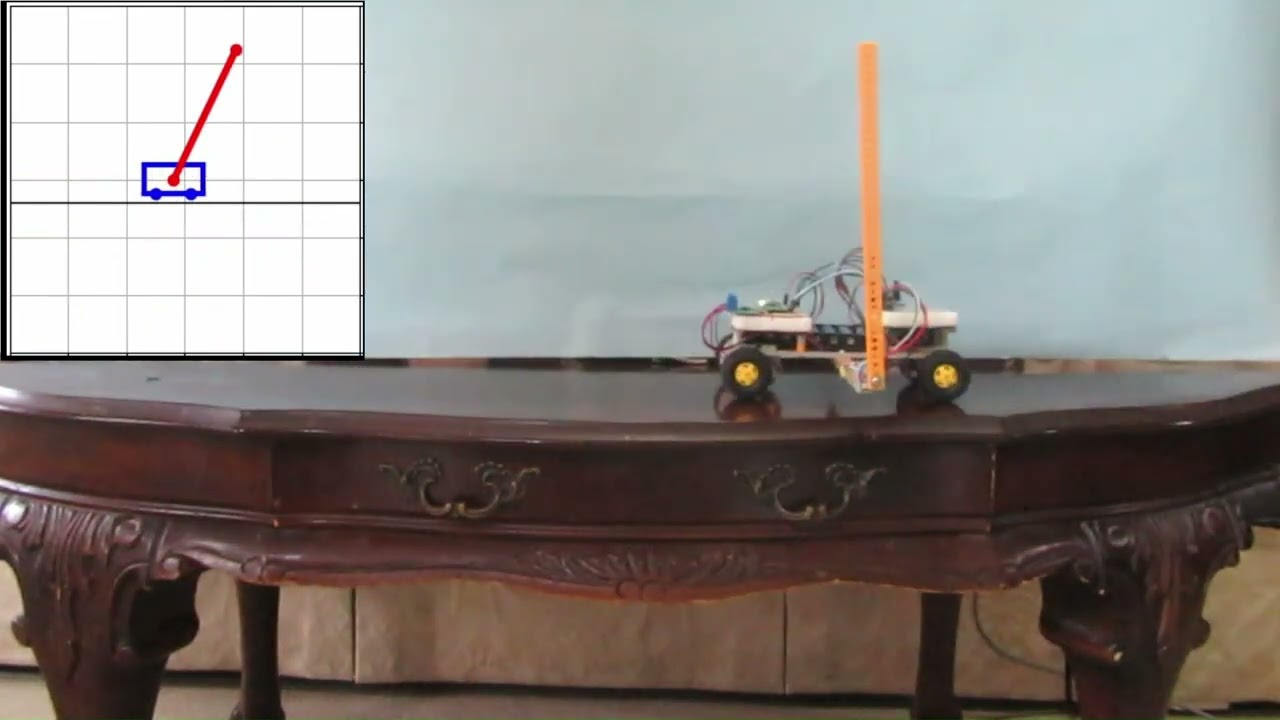
\includegraphics[width=0.48\linewidth]{pictures/youtube/2024/09/20240925_130856_youtube_001_LPguwuZJdAk.jpg}
}
\end{center}




\url{https://youtu.be/UT5q_EeJQ1Q}

\begin{center}
\href{https://youtu.be/UT5q_EeJQ1Q}{
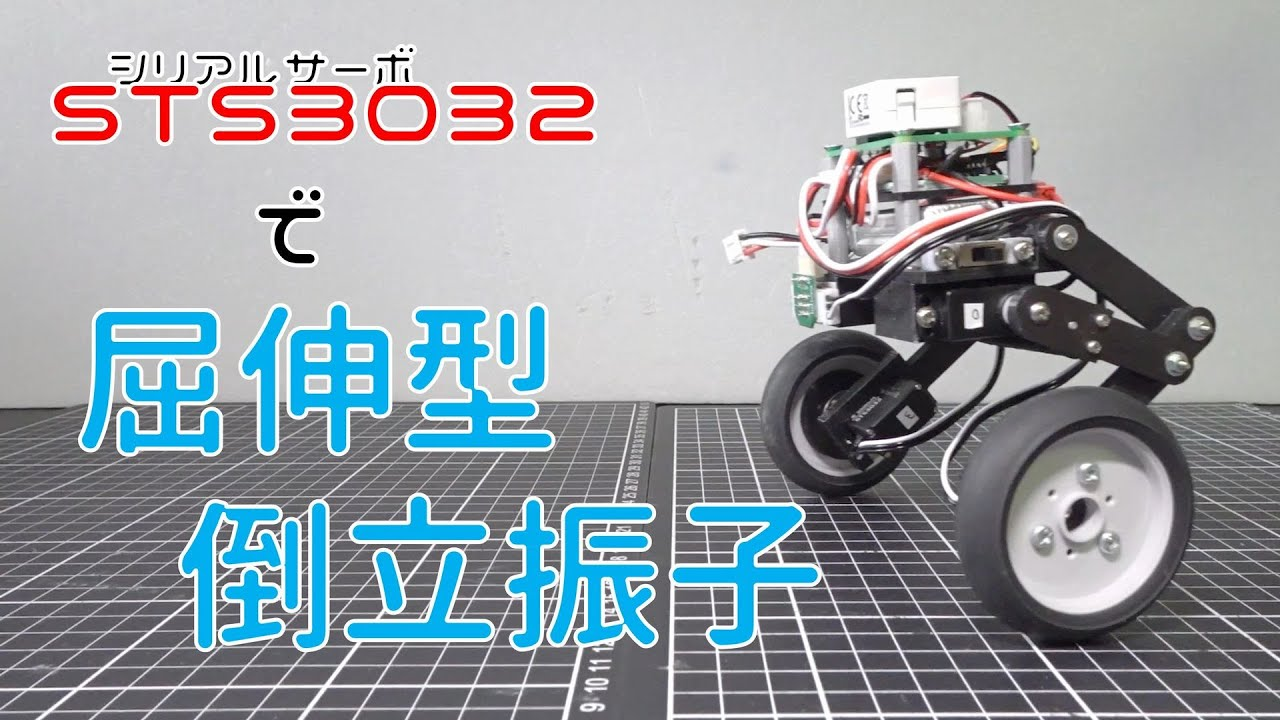
\includegraphics[width=0.48\linewidth]{pictures/youtube/2024/09/20240925_130856_youtube_002_UT5q_EeJQ1Q.jpg}
}
\end{center}




\url{https://youtu.be/Qf6iFE9nyc8}

\begin{center}
\href{https://youtu.be/Qf6iFE9nyc8}{
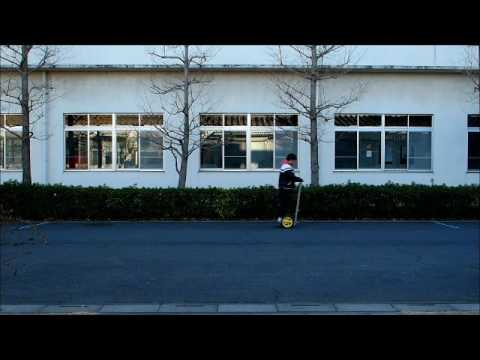
\includegraphics[width=0.48\linewidth]{pictures/youtube/2024/09/20240925_130856_youtube_003_Qf6iFE9nyc8.jpg}
}
\end{center}




\url{https://x.com/carter_control/status/2036060266438566040}




\url{https://youtu.be/9kae-UAME1U}

\begin{center}
\href{https://youtu.be/9kae-UAME1U}{
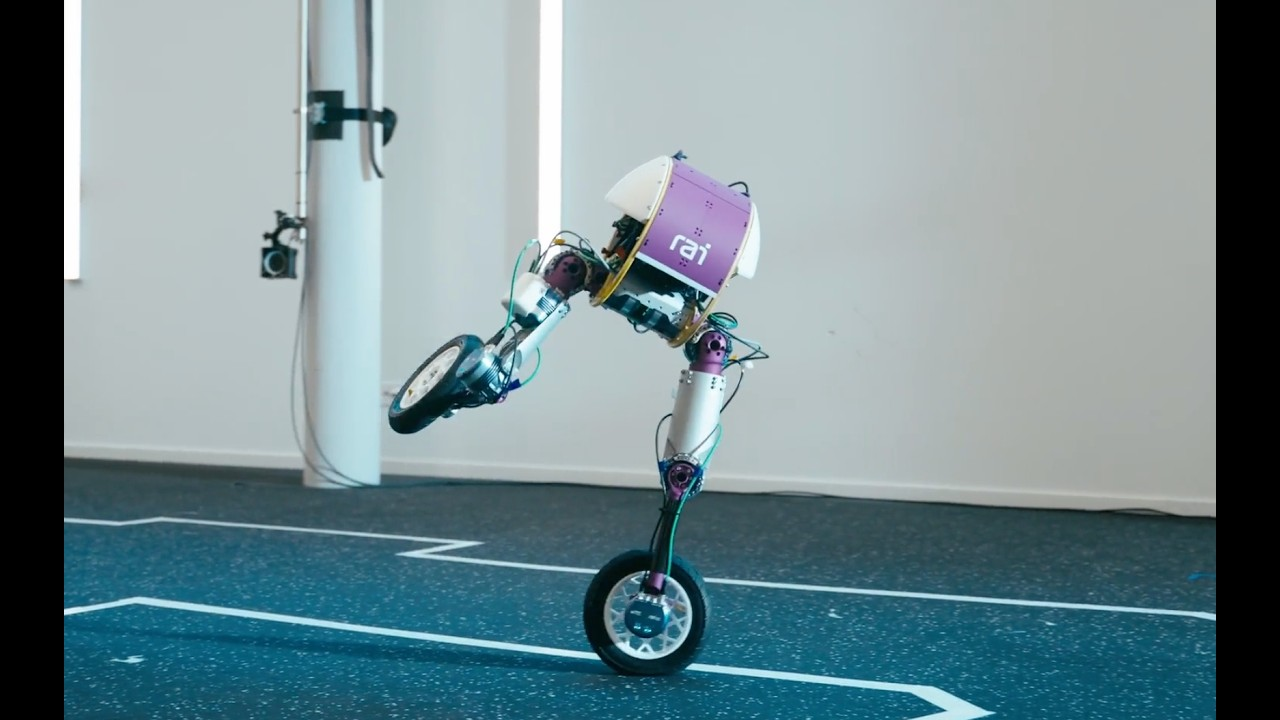
\includegraphics[width=0.48\linewidth]{pictures/youtube/2024/09/20240925_130856_youtube_004_9kae-UAME1U.jpg}
}
\end{center}




\url{https://x.com/wevolverapp/status/2038947251305746850}




\url{https://x.com/maide89699220/status/2039111244532331002}




\url{https://x.com/iliraliu_/status/2043027200853545308}




\url{https://fb.watch/GuOg-oZCds/}




\url{https://fb.watch/GulZVSegSM/}




AIに学習させる？

\url{https://x.com/marurur/status/2042560474349527360}




これは凄いけど私には作れないな

\url{https://youtu.be/wV8ARks0bdA}

\begin{center}
\href{https://youtu.be/wV8ARks0bdA}{
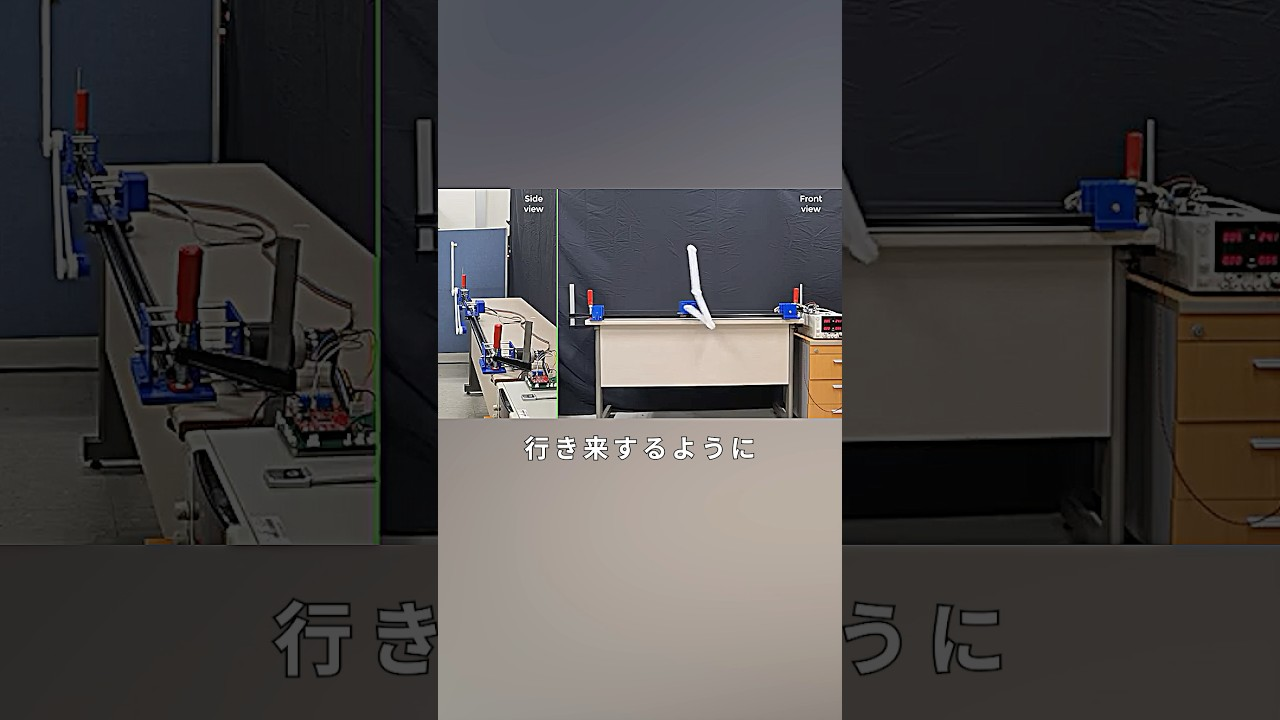
\includegraphics[width=0.48\linewidth]{pictures/youtube/2024/09/20240925_130856_youtube_005_wV8ARks0bdA.jpg}
}
\end{center}



\subsection*{2024年09月26日 09:02}
\addcontentsline{toc}{subsection}{2024年09月26日 09:02}

\#英語検定 のテキストとしてポピュラーな \#旺文社 の「\#文単 （文で覚える単熟語）」を眺めていると、とても有用な表現、感心する様な表現にしばしば出くわします。\#準一級 用の文単を多少なりとも読み進めてきましたが、進めば進むほど、先に読んだページの事を覚えていなくて、右から左へと流れていっているザル状態だと気付かされます。せっかくいいなあと思った箇所があったのに忘れてしまうのはもったいない。かと言って、受験生みたいにノートにえんぴつでゴシゴシ書いて覚えようなど、とてもそんな気にはなれません。


そこで（問題解決になっているかどうかは別にして）、備忘録あるいは学習ノートになる様な、いわゆる \#英語学習アプリ なるものを作ってみることにしました。学習した事を（頭の中にたまっていかないから）データベースにためていこうというわけです。昔Java+ \#mysql 、その後Java+ \#H2DB といった組み合わせで、いろいろ作った経験があるので、\#Java ならデータベースとの接続のイメージを持っていたのですが、今回は \#Python にデータベース「Python+ \#sqlite3 」という、私にとって新しい組み合わせを試してみようと言う気になりました。


できたものは添付画像のとおり。思いのほか小さな規模のプログラムで済みました。Searchボタンの横のコンボボックスから \#検索 項目を選んで検索すると、検索結果のリストが出来上がるので、1stボタン、previousボタン、nextボタン、lastボタンを使って、検索結果をナビして使います。


コレは案外いいんじゃないかと思っているのは、和文蘭、英文欄、ヒント欄のそれぞれに、show/hide のトグルボタンを設けている事です。英文欄とヒント欄をhideにして、show状態の和文を見ながら、自力で英文を考えるとか、必要に応じてヒント欄をshowにするとか、答え合わせで英文欄をshowに戻すとか、便利そうじゃないですか。また、左上のチェックボックスですが、検索結果をランダムに並べ替えて出題するというボタンです。使えそうではありませんか。


添付の画像は、準一級文単の134ページ12行目から始まる英文のお勉強を想定してデータの入力をしてみました。（旺文社の著作権に忖度して）英文欄をhideの状態にしています。もう少しボタンの配置やWindow上の見かけなどを調整したら、そのうちソースプログラムは、いつもの様に \#GitHub にpushしておこうと思います。（入力したデータの方はオープンにできませんね）


今回はPythonでsqlite3という \#DBMS を使える様になったということで、英語の学習そのものは全く進みませんが、プログラミングの学習だけが進みました。やれやれ。

\paragraph{写真}
\begin{center}
\begin{minipage}{0.48\linewidth}
\centering
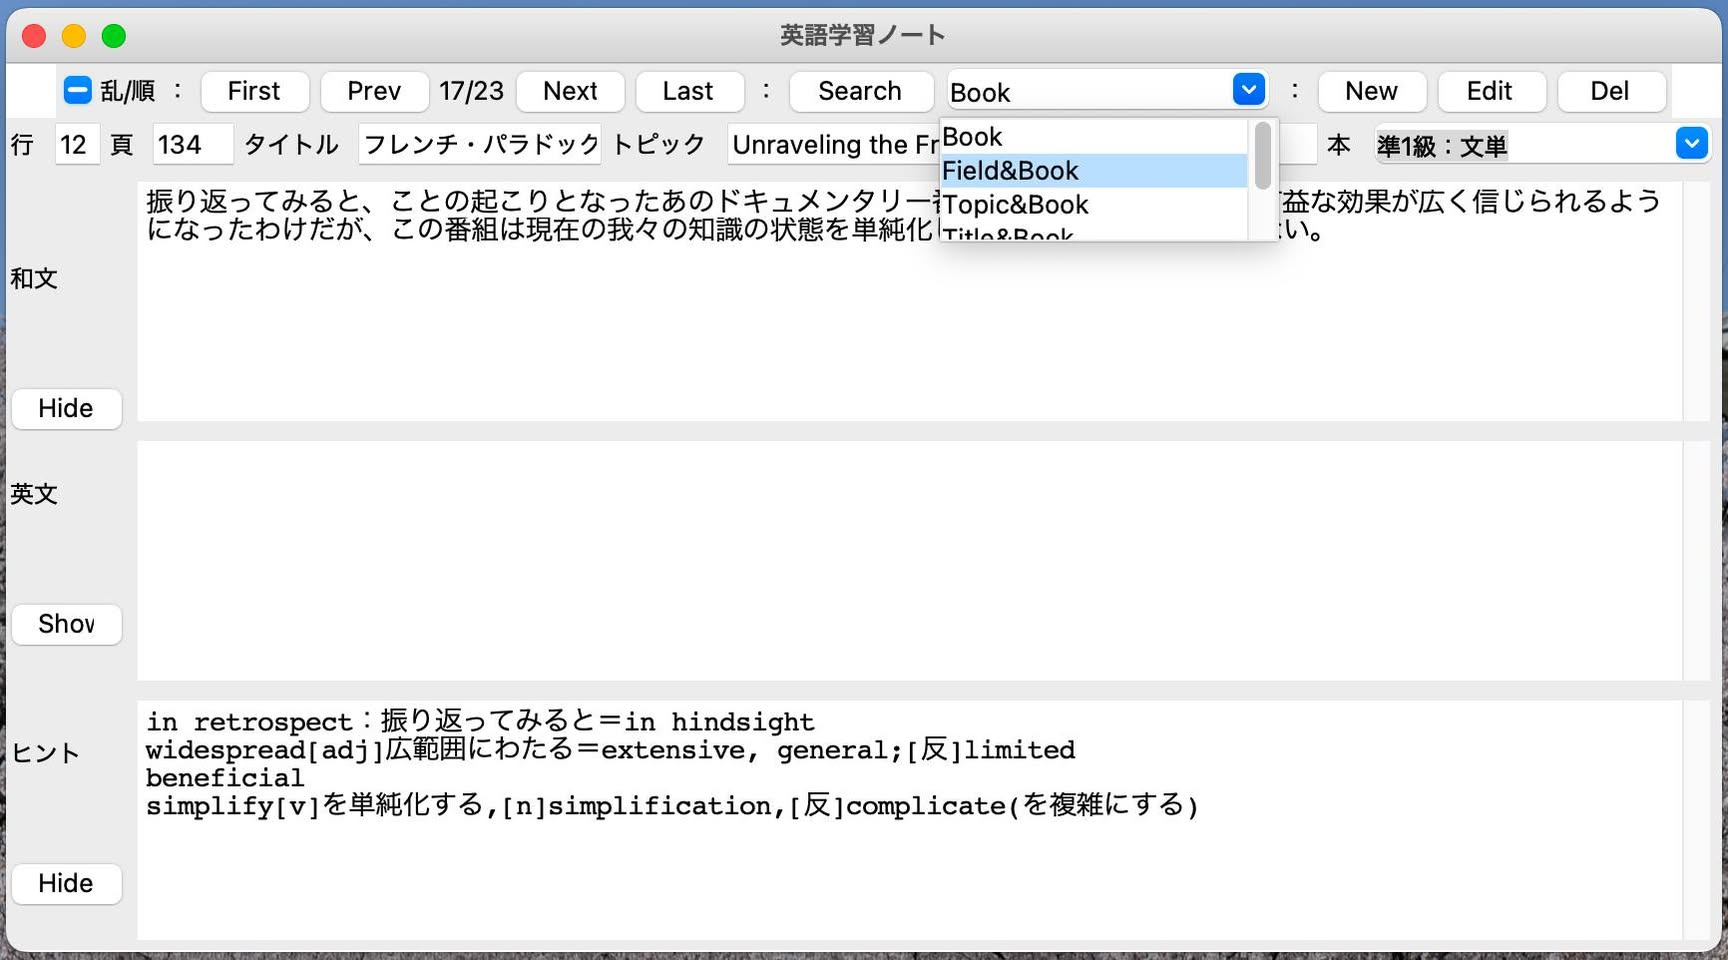
\includegraphics[width=\linewidth]{pictures/2024/09/20240926_090218_001.jpg}
\end{minipage}
\end{center}

\subsection*{2024年09月29日 10:34}
\addcontentsline{toc}{subsection}{2024年09月29日 10:34}

「右」の語釈


「南を向いた時、西にあたる方」（広辞苑）

「この辞書を開いて読む時、偶数ページのある側」（岩波国語辞典）


「舟を編む」（映画、NHKドラマ）を見た時に印象に残りました。（NHKのドラマでは、夕陽を見て涙が流れたのは右の目みたいな事を言ってたけど）


「こんなこと考えて辞書は作られるのか」と思っていた所、ジャパンタイムズ出版の英英英単語という受けん（大学受験や英検受検）用単語帳で同じ場面に遭遇した。例えばたまたま私が持っていた「英英英単語（上級編）」の最初のstageに出てくる単語、例えば、diagnoseとかlegacyとか、普通なら診断とか遺産で済んでしまう所ですが、「問題の原因を見つけること」、とか、「死んだsomeoneから受け取ったsomething」、といった様に、いわゆる語釈に相当することが英文で説明されている。これがとっても面白い。まあ英英辞典を読んでいる感じなのだが、この意味では初級編までも手に入れて、基本的な単語であるほど英語でどんな説明になっているのか読んでみたくなります。


因みに、Oxford英英辞典による「right」の語釈は、「on, towards,or relating to the side of a human body or of a thing which is to the east when the person or thing is facing north」広辞苑と向いている方向が反対（背中合わせ）なんですね。

\paragraph{写真}
\begin{center}
\begin{minipage}{0.48\linewidth}
\centering
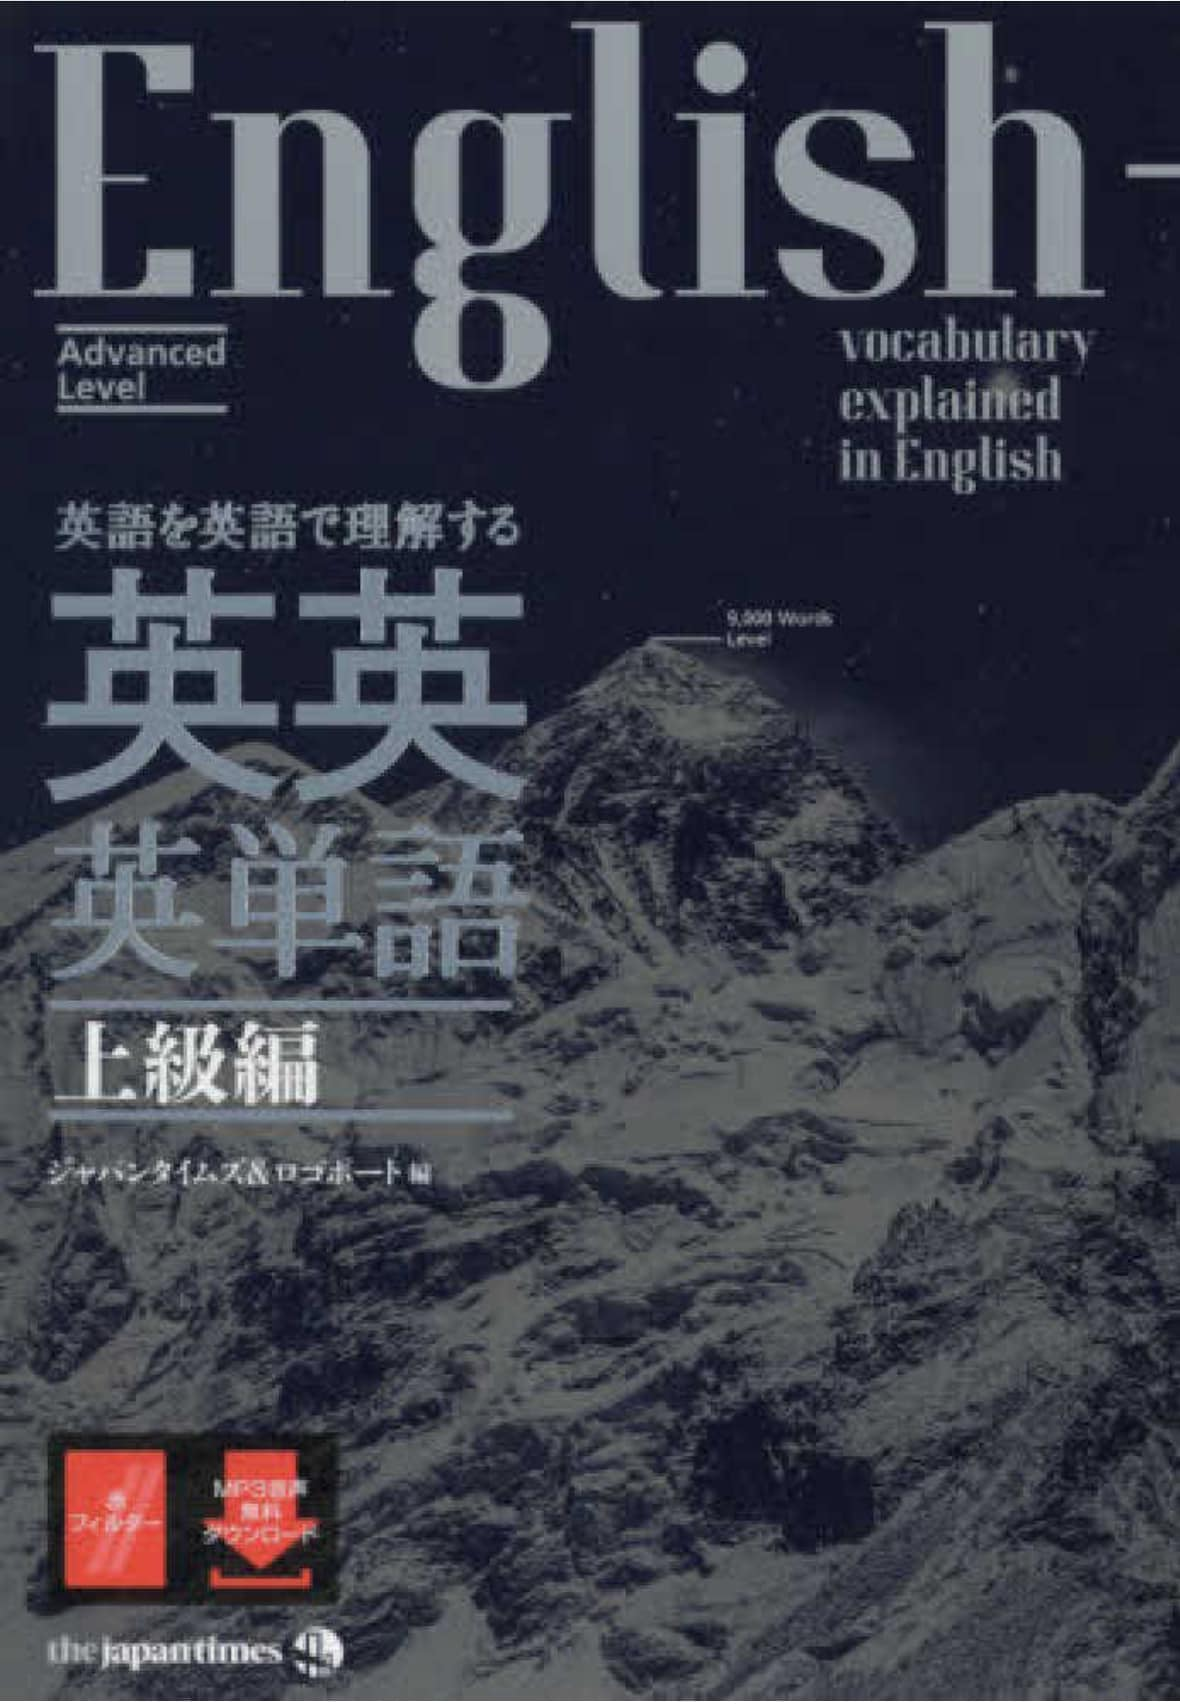
\includegraphics[width=\linewidth]{pictures/2024/09/20240929_103403_001.jpg}
\end{minipage}
\hfill
\begin{minipage}{0.48\linewidth}
\centering
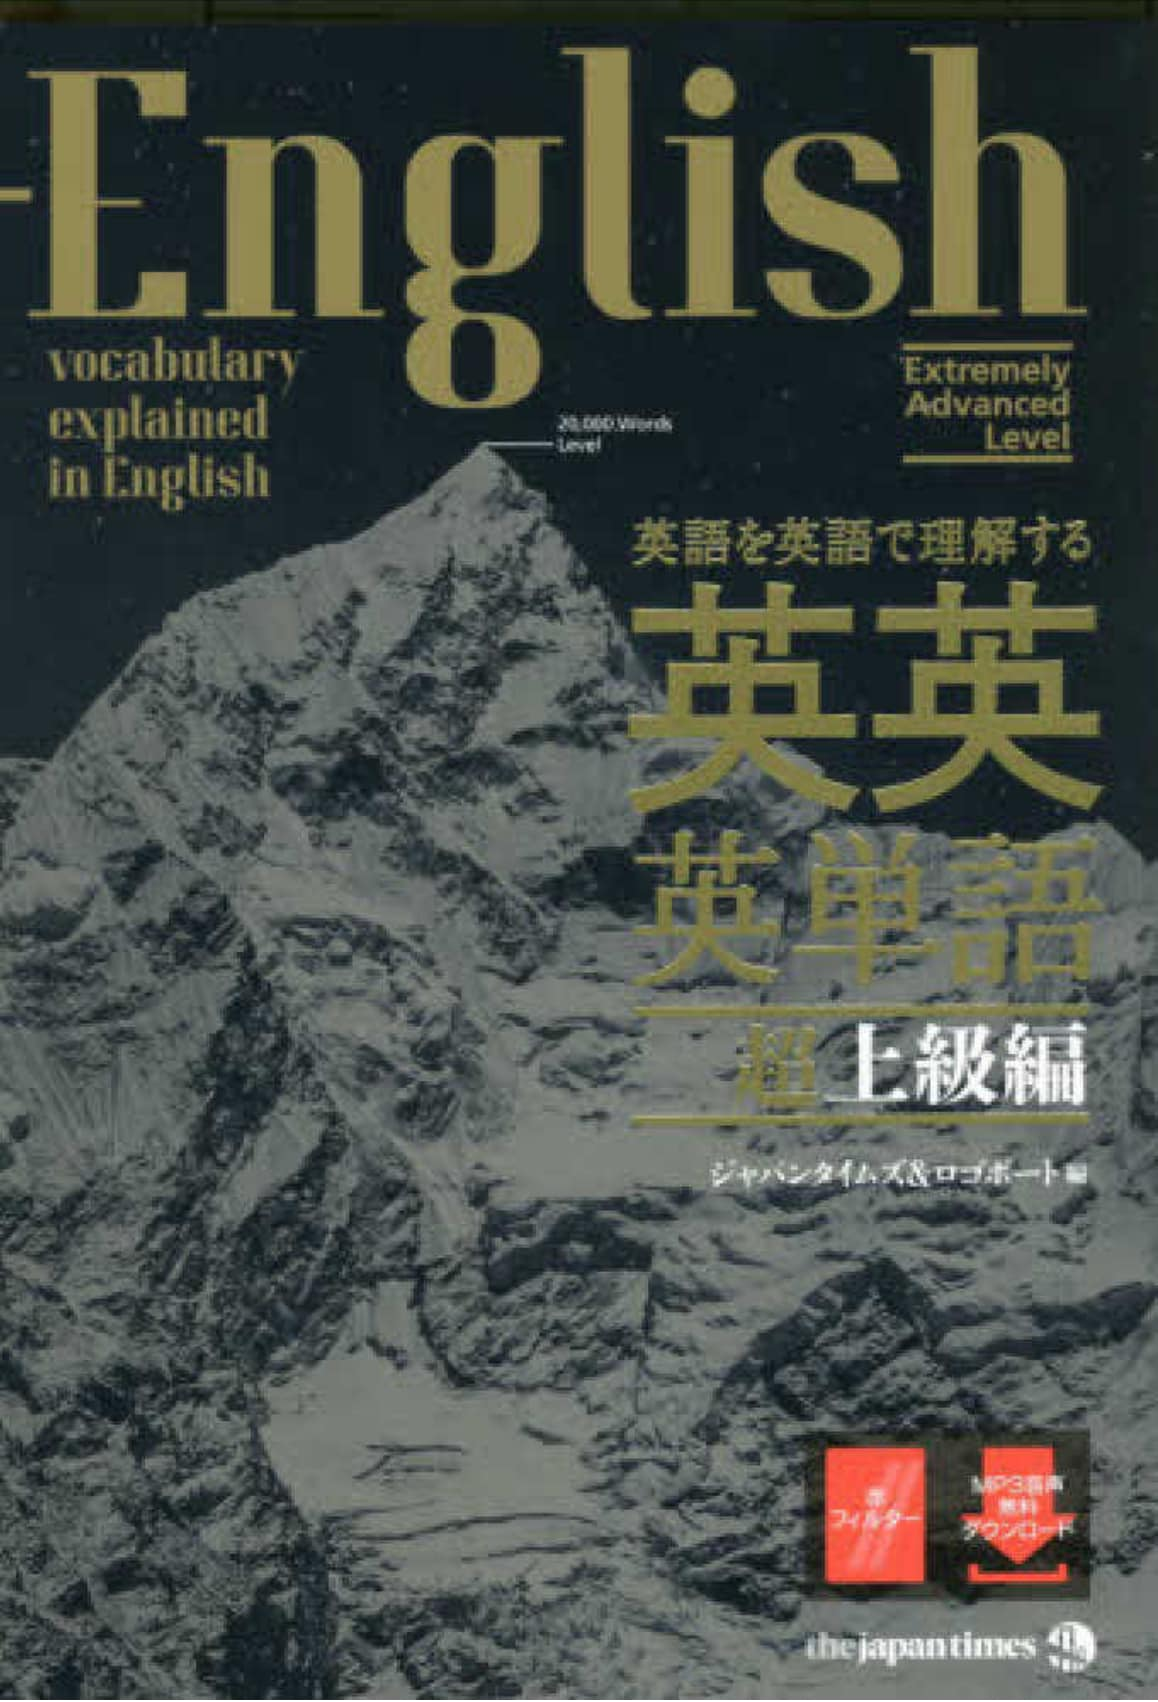
\includegraphics[width=\linewidth]{pictures/2024/09/20240929_103403_002.jpg}
\end{minipage}
\end{center}

\begin{center}
\begin{minipage}{0.48\linewidth}
\centering
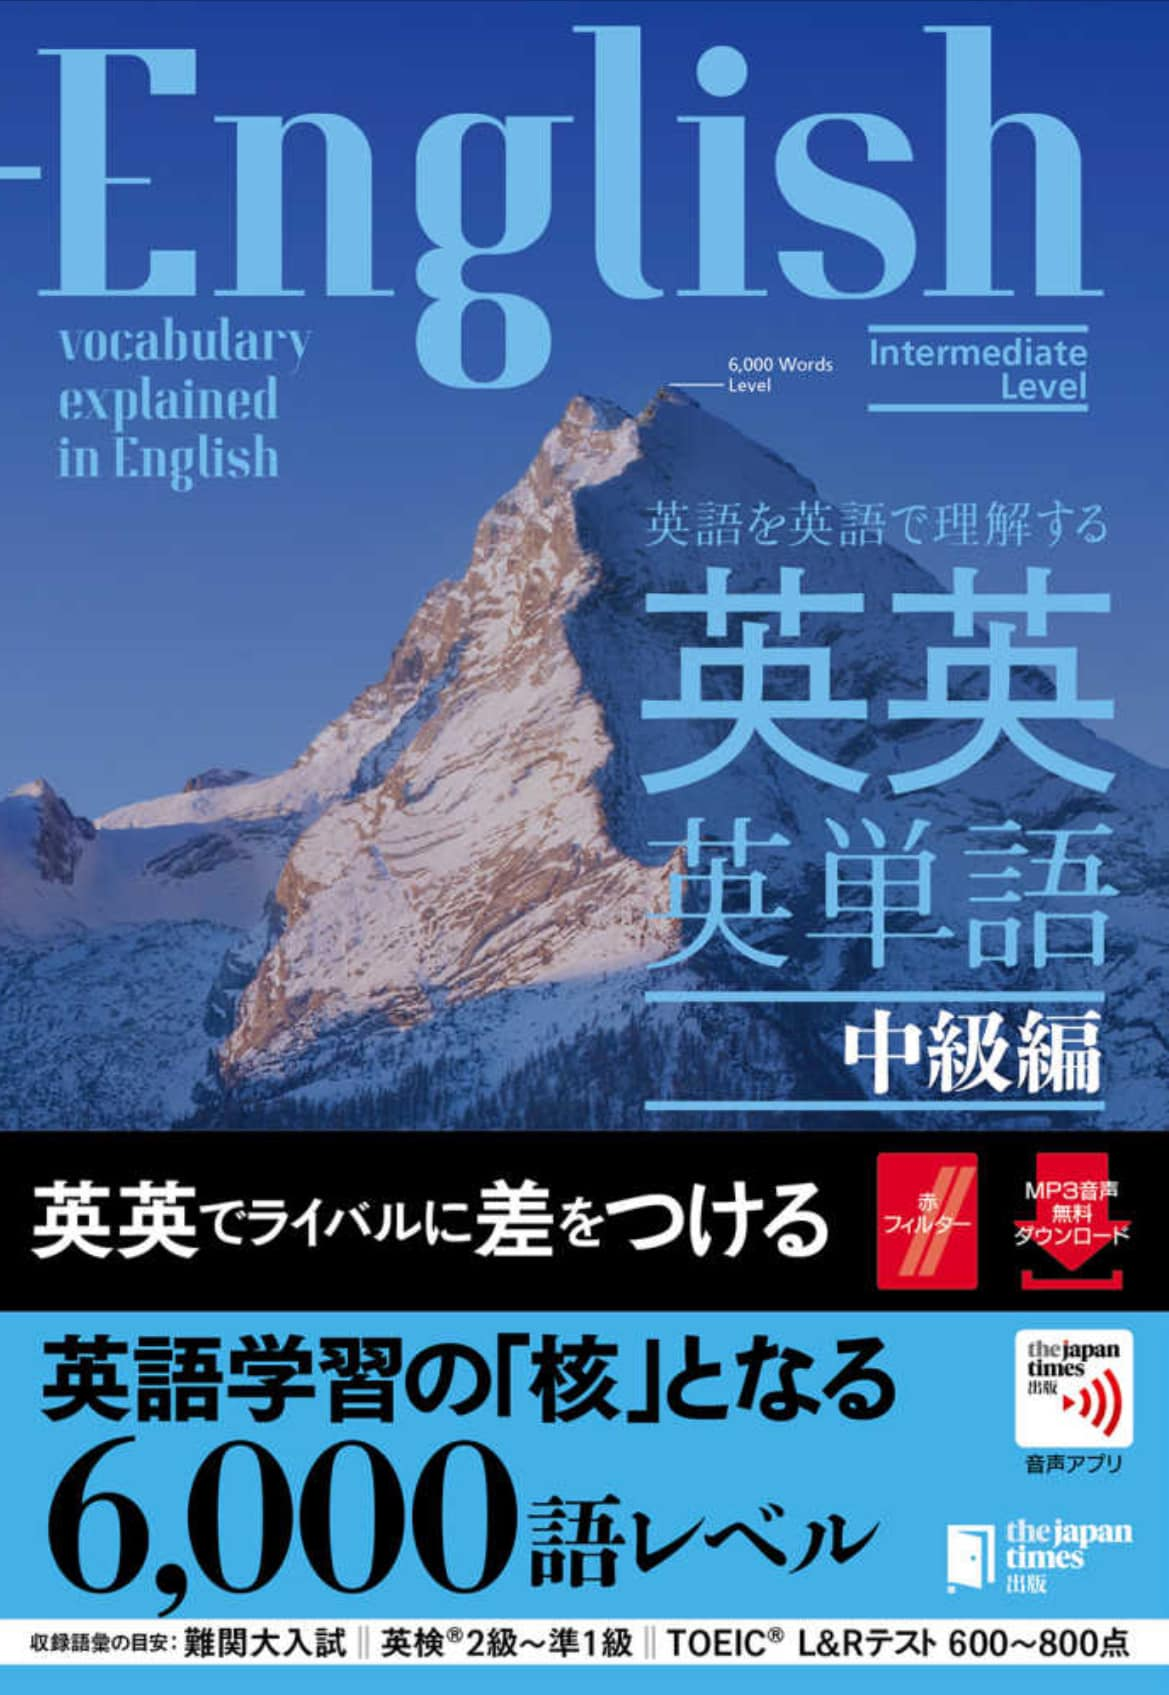
\includegraphics[width=\linewidth]{pictures/2024/09/20240929_103403_003.jpg}
\end{minipage}
\hfill
\begin{minipage}{0.48\linewidth}
\centering
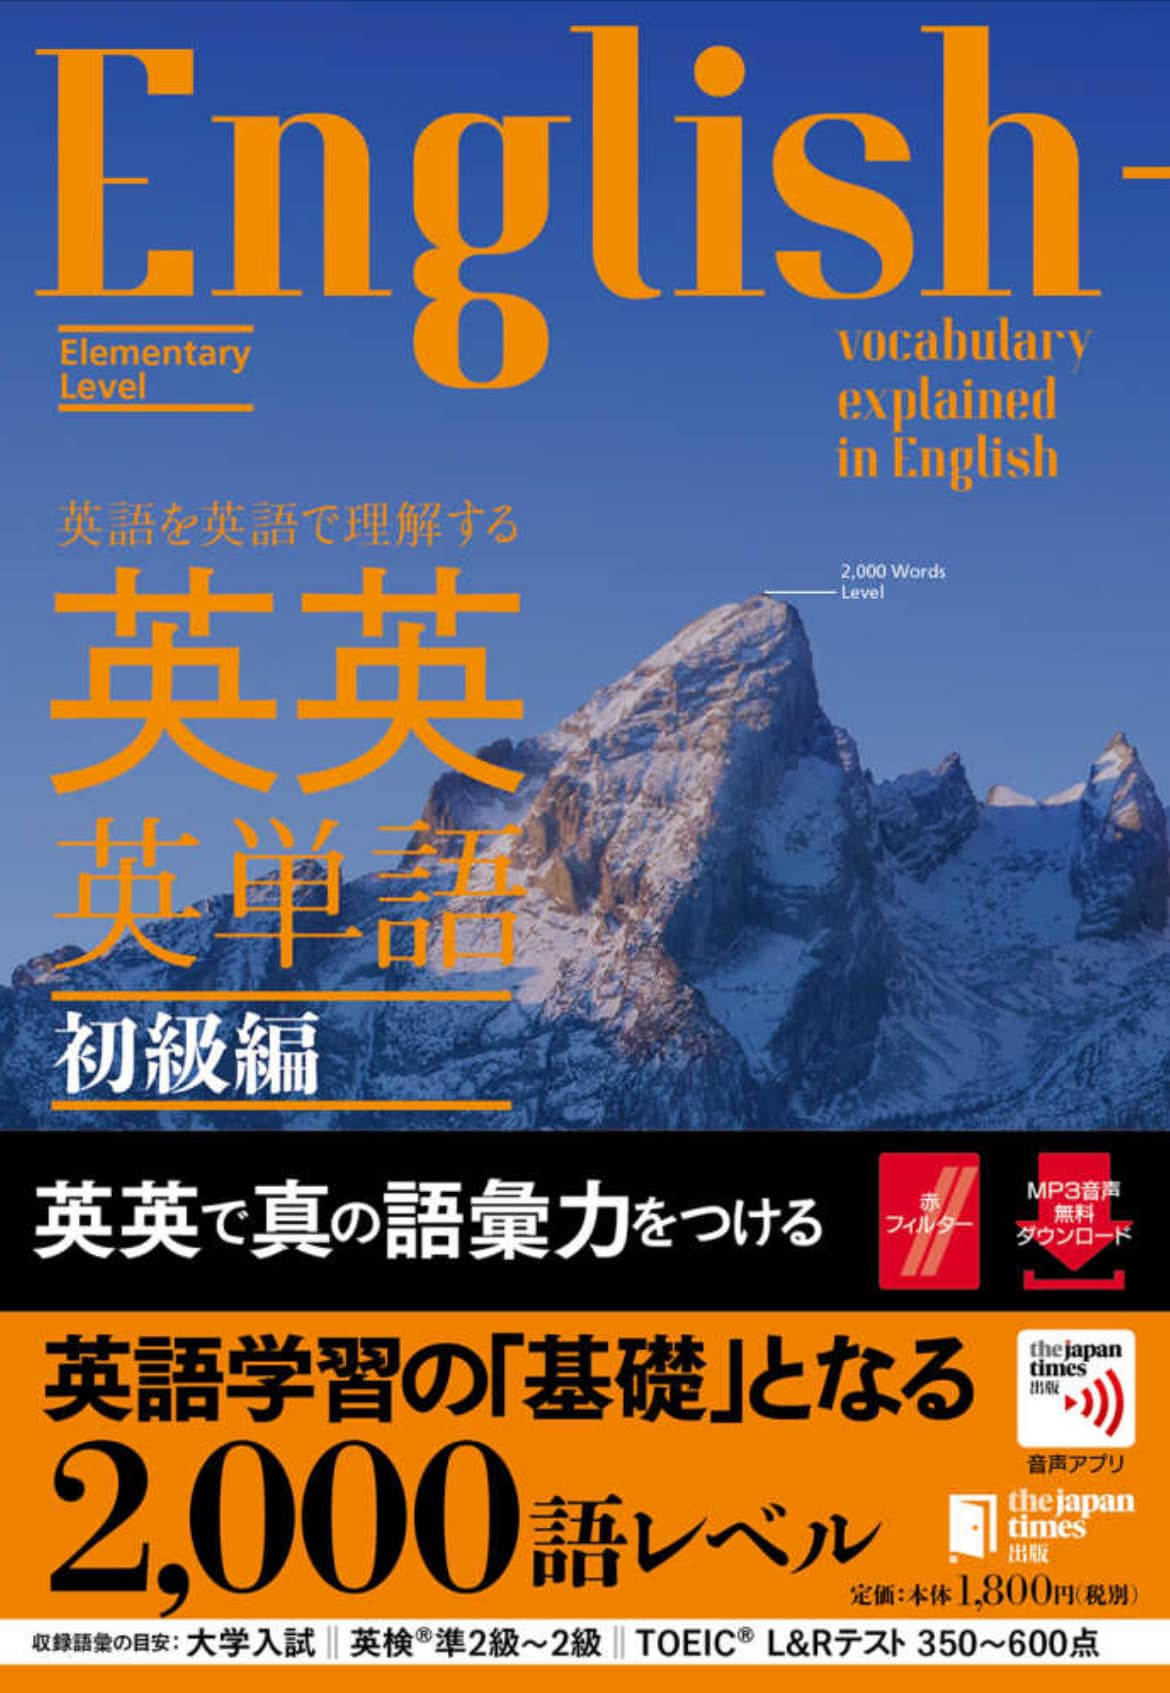
\includegraphics[width=\linewidth]{pictures/2024/09/20240929_103403_004.jpg}
\end{minipage}
\end{center}

\section{10月}

\subsection*{2024年10月02日 06:21}
\addcontentsline{toc}{subsection}{2024年10月02日 06:21}

swift+swiftUI+SQLite3で英単語帳アプリを作ってみているのですが。


以前10年ほど前にプログラムしてみていた時は、swiftUIではなくてUIKitでしたし、SQLite3もFMDB何某をあれこれimportして使っていました。これらは旧来のObjective-Cが持っていたライブラリを流用していたため、比較的複雑なコードになったと記憶しています。


久しぶりにswiftでiOSのアプリに向き合ってみると、新たにswiftUIなるものが登場しており、いろいろ便利になっている様でした。また、嬉しかったのは、import sqlite3の一行でSQLite3を使い始められるという点です。


初めのうちは順調にことは推移してきていたのですが、ほぼ完成かという終盤にきて何と、「TextFieldに日本語の入力ができない！」という事態に遭遇し、このプロジェクトは一旦ストップしています。ネットをググってみると、日本語入力に関してバージョンによっては不具合があるという記事もあったので最新にしてみましたが、日本語入力の問題は最新版においても未解決のままです。ネット上にはUIKitから流用した関数を別途用意して解決しようとしていた方もいらっしゃいましたが、「axis:.vertical」という複数行入力オプションの指定に対応できない様子でしたので利用を断念しました。TextEditを使えばいいのではないかという説もありますが、ここは一旦休止して、TextFieldが対応してくれるのを待とうと思います。（長い間対応できていない様なので、対応するつもりはないのかもしれない＝複数バイト文字って欧米の方からすると面倒でしょうがない代物かと推察します）

\paragraph{写真}
\begin{center}
\begin{minipage}{0.48\linewidth}
\centering
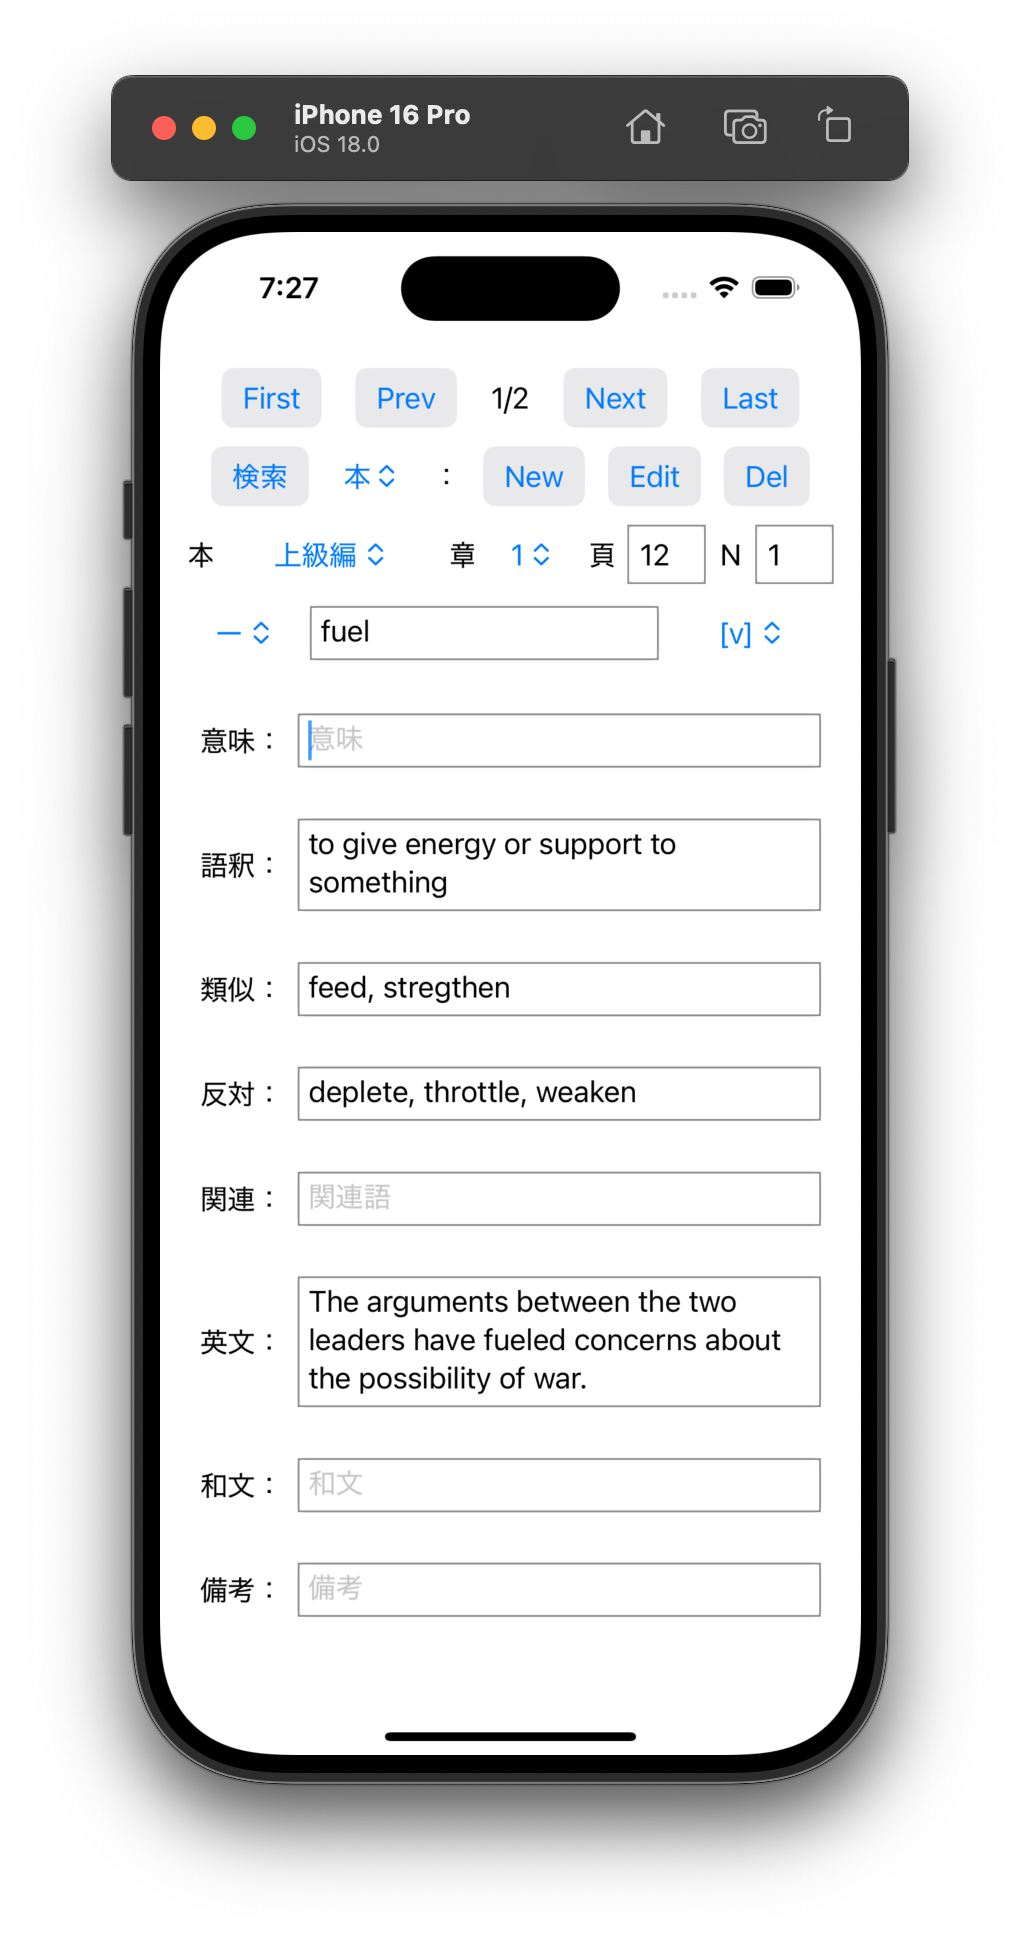
\includegraphics[width=\linewidth]{pictures/2024/10/20241002_062123_001.jpg}
\end{minipage}
\end{center}

\subsection*{2024年10月02日 18:55}
\addcontentsline{toc}{subsection}{2024年10月02日 18:55}

これまでに、次の3種類のデータベースアクセスのアプリを作った経験によれば、最も簡単なのは(２)の場合だ。プログラムが簡単で短くなる理由は、構造体などの定義が不要だからです。


(１)Java + Swing + MySQL（or H2DB）

(２)Python + TKInter + SQLite3

(３)Swift + SwiftUI + SQLite3


もちろん色々な方法がある事にはあるのだろうけど、普通にやるならば、例えば(３)の場合なら、いろんなオブジェクトからなる構造体を定義して、その構造体のインスタンスの配列を作り、そこにSQLのSELECT文によって得られた検索結果を格納して、処理部とやり取りをすることになるでしょう。また、（１)の場合であれば、Collectionフレームワークから例えばListを使ったクラスを定義して、そのインスタンスに検索結果を持たせて、処理部とのやり取りを、そのインスタンスに持たせている関数を使ってする事になる。特にJavaの場合、データベースにアクセスする文をtry-catch-finallyで囲ったりしているから、ますますソースは肥大化する事になる。


ところがPythonの場合はと言えば、構造体の類いを定義する事はない。つまり、何番目のフィールドが整数で何番目のフィールドが文字テキストで、といった事をそれほど気にしなくてもよいのだ。Pythonという「プログラム言語の気持ちになる？」と、暗黙のうちにも「リスト構造が得られるに違いない」と思い込んでいる所があるのだが、実際にSQL（INSERT）で、リスト構造のデータを用意してあげると受け取ってもらえるし、SQL（SELECT）の実行結果を受け取ってみると、期待通りのもの（リスト構造）が返されているので、ちょっと不思議な感じだ。

\subsection*{2024年10月03日 01:10}
\addcontentsline{toc}{subsection}{2024年10月03日 01:10}

\#Swift によるプログラム開発って、かなり敷居が高いという気がする。


そもそも開発環境の \#Xcode だが、メニューなど一部が日本語化されているとは言え、help情報などを見ると画面中至る所英語だらけだ。更に自分で作ったプログラムなのに、自分が購入した iPhone に自由にインストールして使い続けることができない。年会費１万3千いくらを払って開発者のためのアカウントを取得する必要がある。（無料のアカウントでは、プログラムの有効期間は実機にインストールした日から一週間だけ）


自分のプログラムを \#Appストア に公開して、そこからダウンロードして使える様にしようとすると、もっと面倒な事になる（以前にプログラムを公開してみた時の経験です）。必要なことなのかもしれないのだが、 \#Apple 社の審査がある。そもそもそんなアプリを新たに作る必要があるのか？（似た様なアプリなら既に公開されているではないか？）という様な事までもが「英文メールで」問い合わせが来る。当然の様に「英文メールで」理由をつけて言い訳しなければならない（はあ、疲れる）。以前は私にとってはどうでもいい様な機能を付加価値の様に追加して、Appストアへの公開理由を捻出した経験がある。

また、何らかの不都合な動作がある場合、例えば動作する対象のデバイスをiPhoneと \#iPad の両方にしていると、旧いiPadによっては画面上での体裁が悪くなっていたりする事がある。そんな場合にもやはり英文メールで指摘されるので、対象機種を限定してmakeしたり、 \#iOS のバージョンを限定する修正をしたりして英文メールで回答する、といったやり取りを何度か繰り返して、ようやく自分で作ったプログラムを公開できる様になる。そして、公開したらしたで、その後のiOSのアップデートに追随して自分のアプリもメンテし続けていかなければならない。（私が昔公開したアプリは全くメンテしてこなかったので、とうの昔にAppストアから姿を消していますし、そもそも年会費の支払いをやめていたので、開発者アカウントも失効しています）

何にせよ、これらの事はプログラムを身近で使おうと思っている日曜プログラマにとって、本当に敷居の高い事だと思います。（実際は、Appストアに公開しなければ、年会費の負担だけになるという事なのですが）

こうして見るとApple社は本当にキチンとAppストアを運営しているのだという事が分かります。ストアがゴミだめになっていかない様に。


因みに \#Android 端末のアプリ（これは \#Java で開発できる）の場合、自分で作ったプログラムの公開は特に何のやり取りもなくできていました（昔の話です）。今は状況が変わっているかもしれません。


という事で、以前持っていたAppleの開発者用アカウントは既に失効しているのですが、新たに取得し直すのはやめて、シミュレータでプログラムの動作を確認しているだけです。（しかし、何となくSwiftのプログラムを作る事が虚しいことの様に思えてきます。単なる時間潰しですね。何やってるんだか。）

\subsection*{2024年10月05日 09:44}
\addcontentsline{toc}{subsection}{2024年10月05日 09:44}

応援中: Siccas Guitars ―ライジングファンに認定されました！🎉

\paragraph{写真}
\begin{center}
\begin{minipage}{0.48\linewidth}
\centering
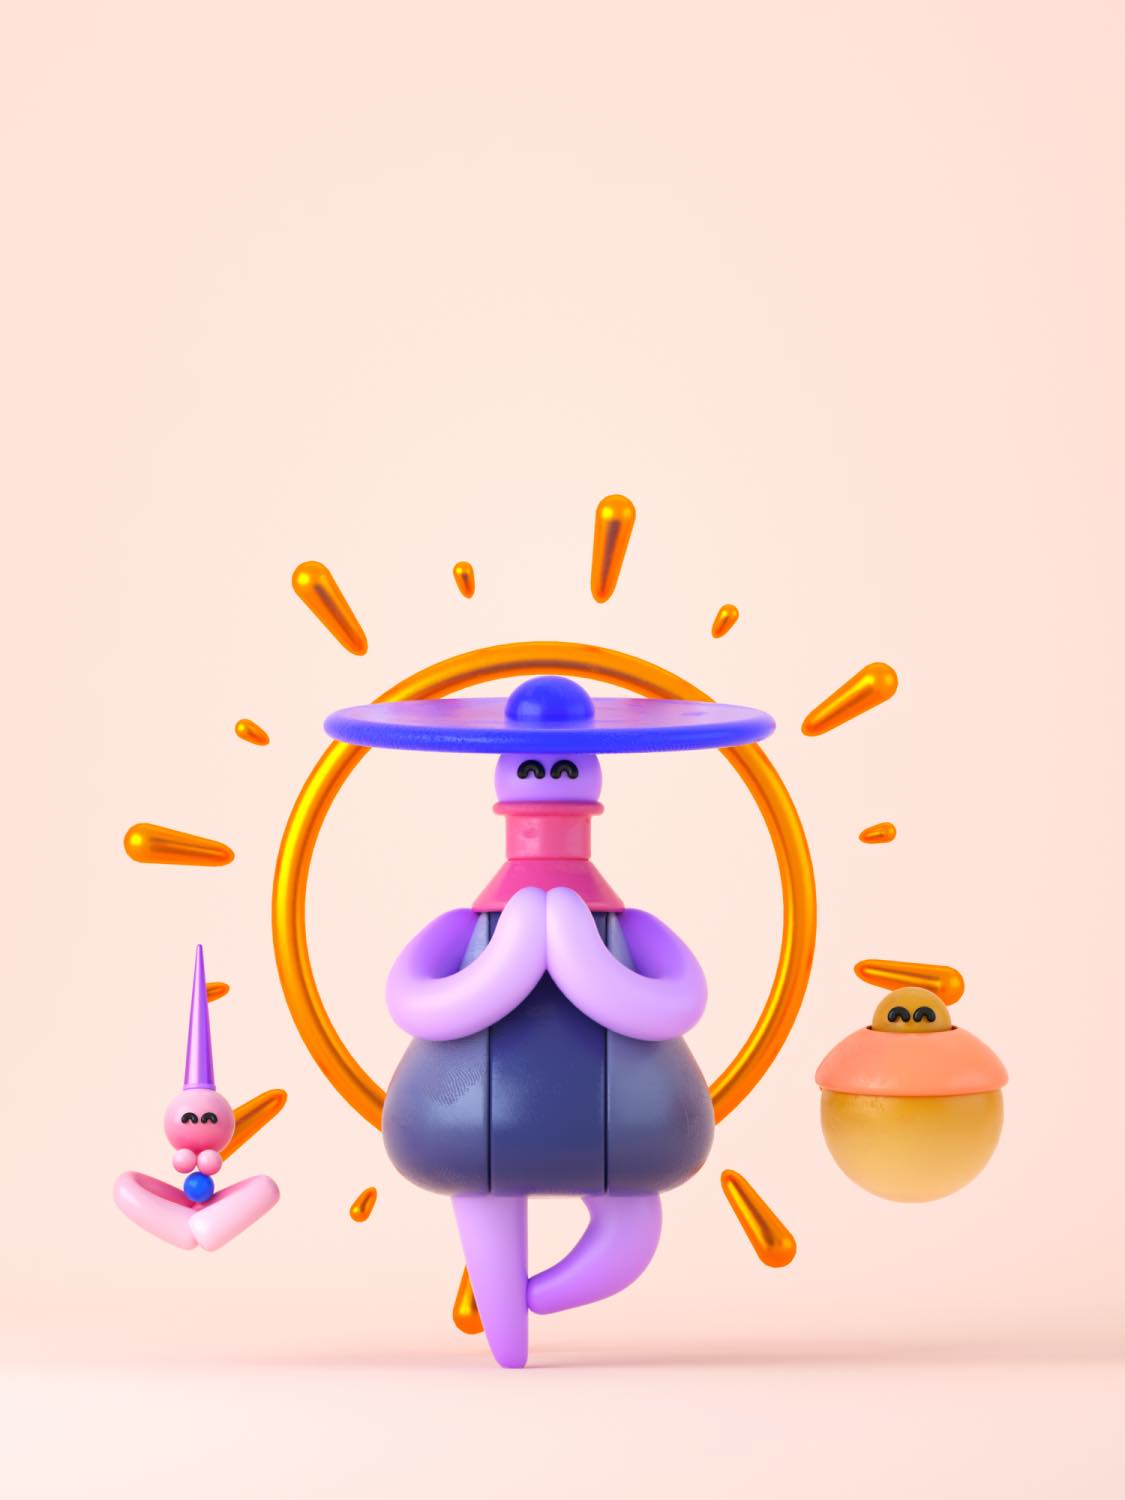
\includegraphics[width=\linewidth]{pictures/2024/10/20241005_094404_001.jpg}
\end{minipage}
\end{center}

\subsection*{2024年10月05日 21:24}
\addcontentsline{toc}{subsection}{2024年10月05日 21:24}

\url{https://youtu.be/lxZqC_J0C74}

\begin{center}
\href{https://youtu.be/lxZqC_J0C74}{
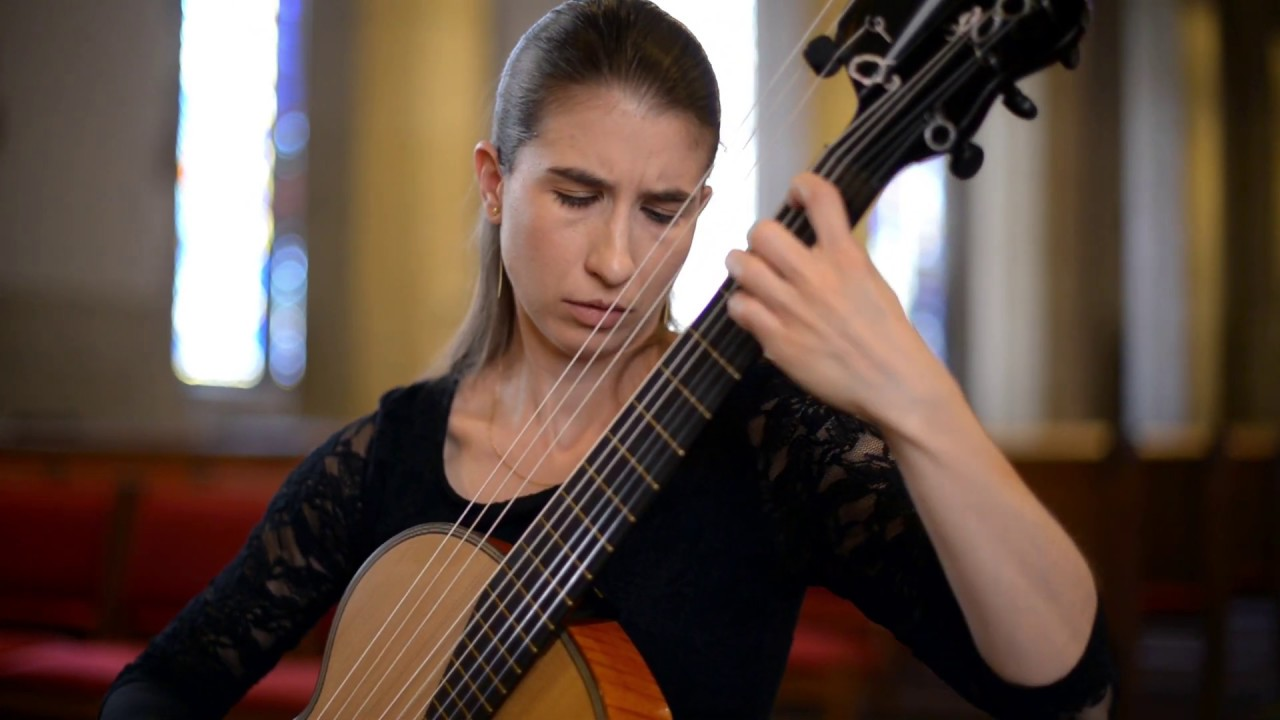
\includegraphics[width=0.48\linewidth]{pictures/youtube/2024/10/20241005_212439_youtube_001_lxZqC_J0C74.jpg}
}
\end{center}




すごくいいですね。何と言っても、この楽器がシャコンヌにピッタリの音してます。速い動きの部分も一つ一つの音がとてもクリアに鳴っています。そして、低音の声部が（乱暴でなく）聞こえているし、内声部の旋律も綺麗に歌っている。後半終わりの方でのアルペジオの（1弦の5フレットのAを鳴らし続ける）あたりなどでは、今まで聞いたギター編には無かった新鮮な演奏でした。すごく気に入りました。今日は何度も何度もこの演奏繰り返して聞いていましたよ。

\subsection*{2024年10月05日 21:25}
\addcontentsline{toc}{subsection}{2024年10月05日 21:25}

\paragraph{リンク}
\url{https://youtu.be/d1_b_Isdelw}

\begin{center}
\href{https://youtu.be/d1_b_Isdelw}{
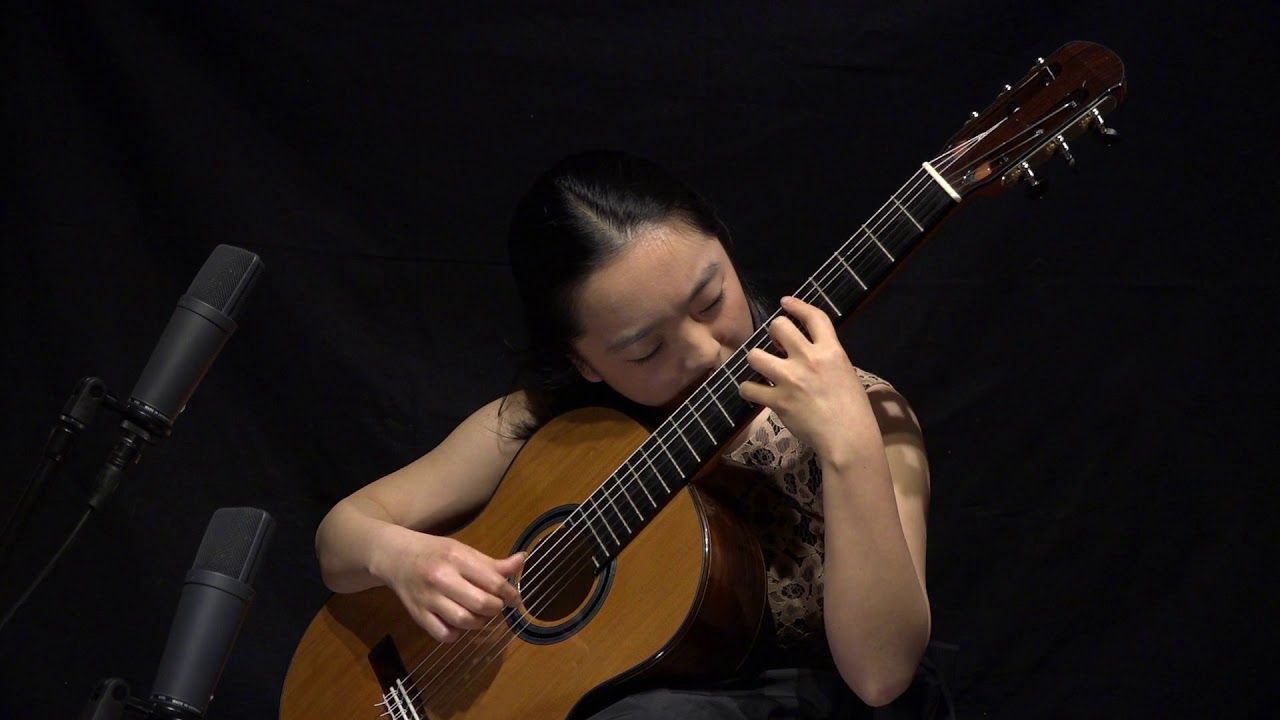
\includegraphics[width=0.48\linewidth]{pictures/youtube/2024/10/20241005_212534_youtube_001_d1_b_Isdelw.jpg}
}
\end{center}

\subsection*{2024年10月11日 11:49}
\addcontentsline{toc}{subsection}{2024年10月11日 11:49}

iPhone のための「英英」英単語学習アプリの開発を（なんとなく思いついた時に）続けている（英語そのものの学習はできていない）。このアプリはジャパンタイムズ出版社の「英語で英語を理解する英英英単語」を使った学習を想定しています（英文による単語の語釈欄を設けているというだけで、他の単語帳のデータでももちろん利用Ok）。基本的に、自分で覚えておきたい単語とその使用例などを登録していく事で学習を進める、自作ノートの様に使いたいと考えています。


(１)

検索結果をナビするボタン（Prev, Next）ですが、画面の1番上に置いていました。でも、寝転んでアプリを眺めていたら、下にあった方が操作しやすいかなと思う様になり、ナビボタンは画面の1番下に配置し直しました。

(２)

これで完成にしようかと思ってカミさんに見せてみた所、何と、指で画面を左右にフリックしようとして「何も動かない」みたいな事を言うので、画面上の左右へのフリック操作でも検索結果のナビができる様にしました。できてみると、これがなかなか操作性が良い様です（ナビボタンは不要かもしれない）。受験生なら電車の中で片手で操作（右手親指で左右フリック）しながら学習する事もできますね。

(３)

また、DBの内容をCSV形式でiCloud上に保存したり、或いはそのCSVファイルを読み込んでDBを再構築したり、データを追加したりできる様に機能を拡張しました。iPadにインストールしたアプリ上でデータ入力したものをCSVにexportし、一方でそれをiPhoneにインストールしたアプリへimportして、コンパクトに持ち歩くこともできる様になりました。もちろんexportしたCSVデータをExcelに読み込ませて再利用する事もできますね（便利便利）。もし仮に受験生が利用するなら、お友達の入力したデータをimportするなどという使い方をしたのでは「お勉強」になりません。自分が問題意識を持った（気になった）単語を登録参照するという作業そのものに意味があるという考え方でのアプリですから。


実はCSVデータの読み込み部分についてはちょっと苦労しています。フィールドデータの中にカンマや改行文字が含まれているものは、実際には区切り文字ではないんだよ、という事を上手にプログラムしてあげる必要がありますから。どこかネット上に、CSV操作のクラスなど落ちていても良さそうな気もするのですが。かなり昔の事ですが、JavaでもCSV読み込みのプログラムを苦労して書いた事がありましたから、今回もゼロから書くことにしたというわけです。（自分の決めたルールで書き出したデータを自分で読み込むということであれば、汎用的なCSVクラスである必要はないのだから。但し少なくともExelには正しく解釈してもらえるレベルである必要はあります。）


※これまでの関連する投稿


(１) iPhoneの英語学習用アプリについて（今回の記事はこれの続きです）

\url{https://m.facebook.com/story.php?story_fbid=8336041646479923&id=100002225117991}




(２) ジャパンタイムズ出版社の本について

\url{https://m.facebook.com/story.php?story_fbid=8310170562400365&id=100002225117991}




(３)Swiftによるプログラム開発について

\url{https://m.facebook.com/story.php?story_fbid=8342998949117526&id=100002225117991}




(４)Pythonによる英語学習用アプリについて

\url{https://m.facebook.com/story.php?story_fbid=8281916311892457&id=100002225117991}



\subsection*{2024年10月12日 06:27}
\addcontentsline{toc}{subsection}{2024年10月12日 06:27}

今回 \#iPhone の \#アプリ を開発するにあたって \#Swift でプログラムを書いていると、気になる事がたくさん出てきた。なぜstructなのか（classではダメなのか）。関数の戻り値は書かなくてもいいのか。ドットから書き始める（ついで書きの様な)書き方はいったい何なのか。一体どこまでがクラス定義で、どこでインスタンスを作っている事になるのか（インスタンス変数とクラス変数はどうしているのか）。どんなタイミングで画面を書きかえているのか。などなど。いろいろ？？な事が多いので、ちょっと本を見てみようと言う気になりました。


添付の本を（Kindleですが）入手して所々眺めていたところ、どうもstructも変数もみんなクラスだと言っている様にみえます。例えば変数への値の代入は変数のセッターが受けとっている様ですし。ただ一方でclassという書き方も存在している様ですし。真正面からSwiftの文法を学ばなくちゃいけないだろうか。まだまだ五里霧中ですけれども、添付の本のキャッチコピー＜現状脱出マニュアル＞「脱出だ！！雲を突き抜けろ！」はとてもキャッチーですね。気に入りました。まさに脱出したい気分です。


だんだん、Swiftというプログラム言語はちょっと面白いのでは、という気にもなってきました。

\paragraph{写真}
\begin{center}
\begin{minipage}{0.48\linewidth}
\centering
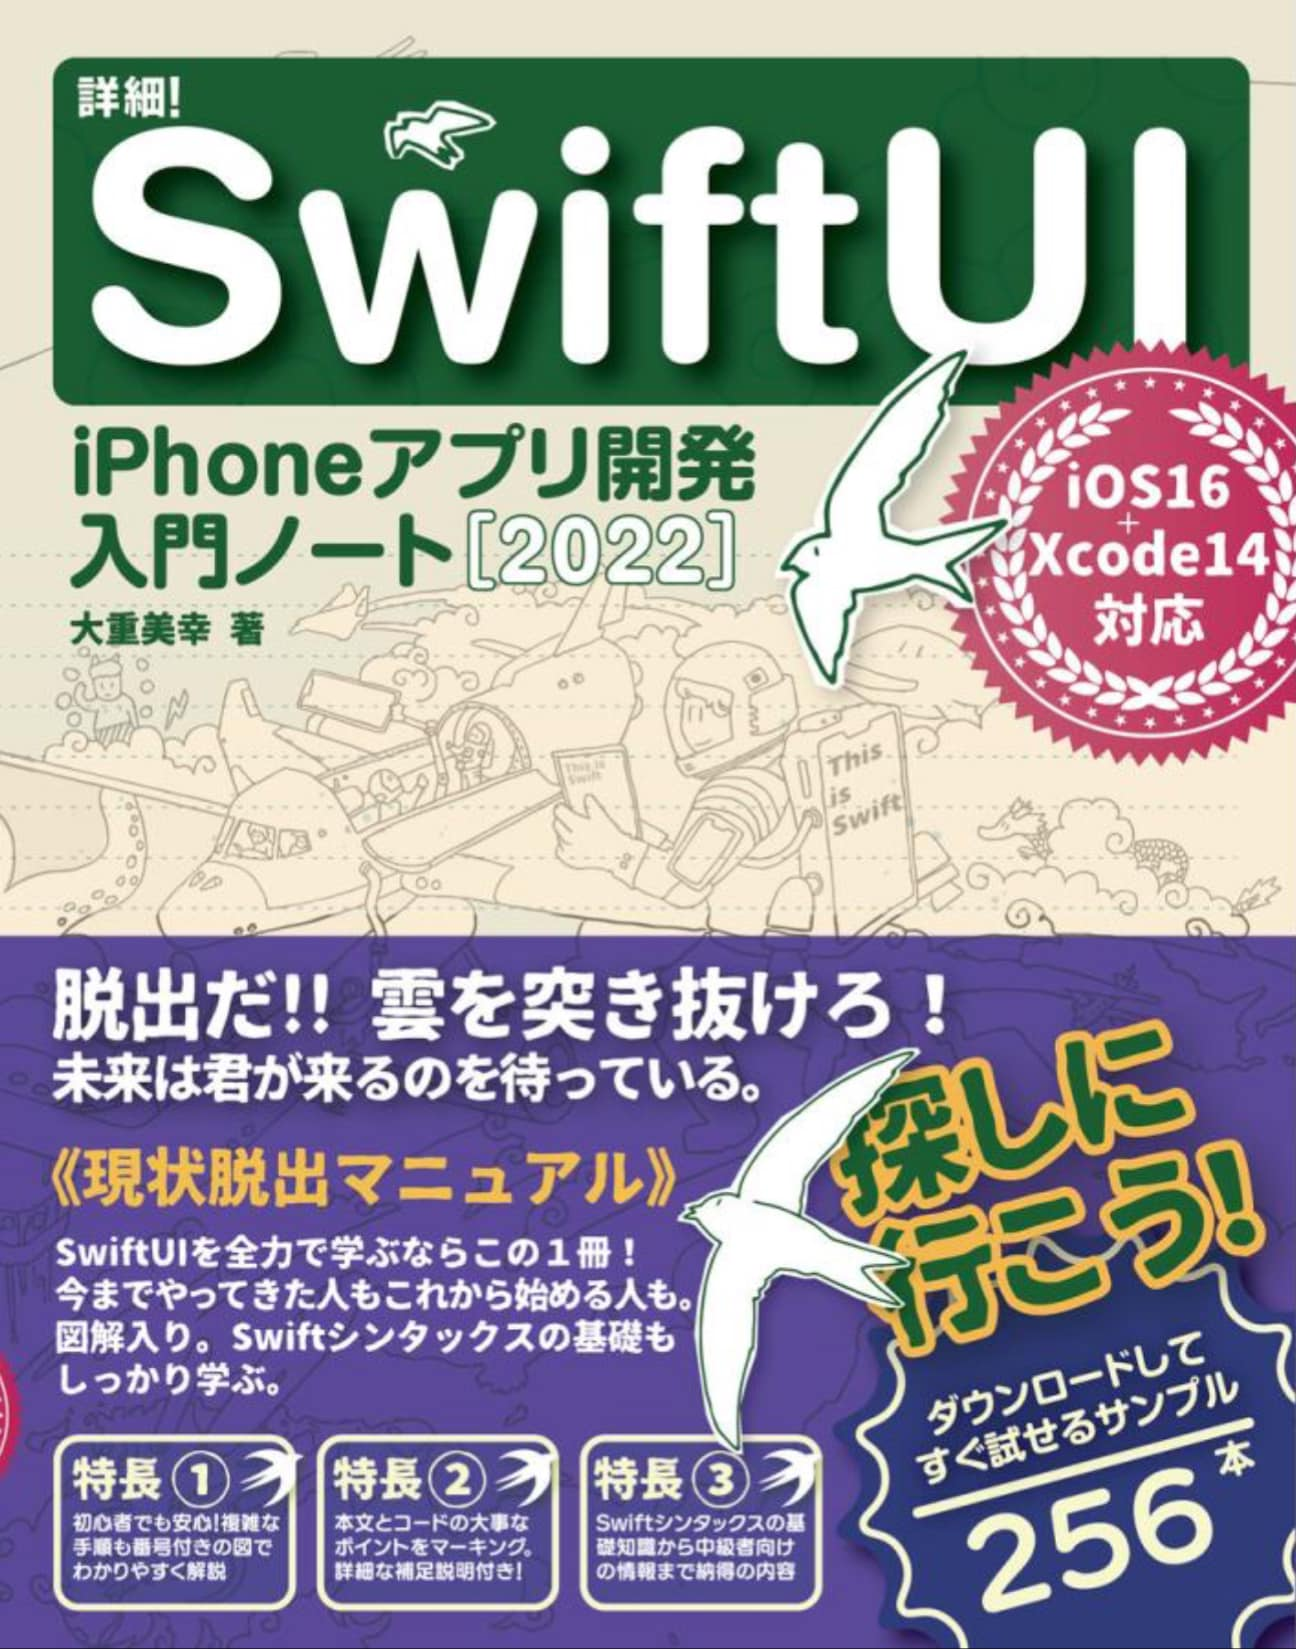
\includegraphics[width=\linewidth]{pictures/2024/10/20241012_062733_001.jpg}
\end{minipage}
\end{center}

\subsection*{2024年10月16日 09:12}
\addcontentsline{toc}{subsection}{2024年10月16日 09:12}

その後の \#iPhone 用. \#英語学習アプリ 製作記です。


英作文学習用と英単語学習用の２つを作ってみました。

画面の \#スワイプ 操作で表示するレコードのナビを実現しているので、ナビのためのボタンPrev,Nextなどは、一番下に置いているとスワイプ操作の邪魔になってしまいます。画面上の一番上に戻しました。

英作文学習用では、各表示欄に「表示と非表示の \#トグル ボタン」を設けています。英文欄を隠して自分で作文してみて、表示ボタンを押して確認するという様な利用状況を想定しています。


添付の図は、英作文学習用ではジャパンタイムズ出版社の「準1級英作文問題完全制覇」を、また英単語学習用ではやはりジャパンタイムズ出版社の「英語で英語を理解する英英英単語上級編」の中のものを表示しているところです。（非表示にしている英作文できますか？答えが気になる様ならジャパンタイムズ出版社の準1級英作文問題完全制覇を手に入れて70ページを参照してくださいね。）


少しずつですが、 \#Swift + \#SwiftUI の使い方が分かってきました。

でも、このプログラム言語はあまり好きになれません。何となく綺麗に書けません。ダラダラと繋がった読みにくいソースになってしまう様な気がします。ダラダラするのはUIを書く時の宿命か、或いはただ単に私のSwiftに関する力量不足が原因なのか？


CSV入出力の処理の問題も上手く解決できないでいます。フィールド内のデータに改行文字を含んだ場合でも、ダブルクゥオートで挟んで出力したらExcelやNumbersでは期待通りに（改行文字もそのままに）読んでくれるのに、その同じデータを自分のプログラムで読もうとするとうまくいかない。改行文字を¥¥nなどの文字で置き換えてしまえばもちろん読み込めるのだが、改行文字そのままで取り込むにはどうしたらいい？よわった事態に陥っている。（改行文字を別の¥¥nなどの文字に置き換えて読見込んでしまって、読み込み終わった後ですぐに¥nに戻せばいいのか？或いは改行文字のままで読み込んで、dbにinsertする前にデータを整形し直すか？）


今回の投稿は、以下の記事の続きです。

\url{https://m.facebook.com/story.php?story_fbid=8420667494684004&id=100002225117991}



\paragraph{写真}
\begin{center}
\begin{minipage}{0.48\linewidth}
\centering
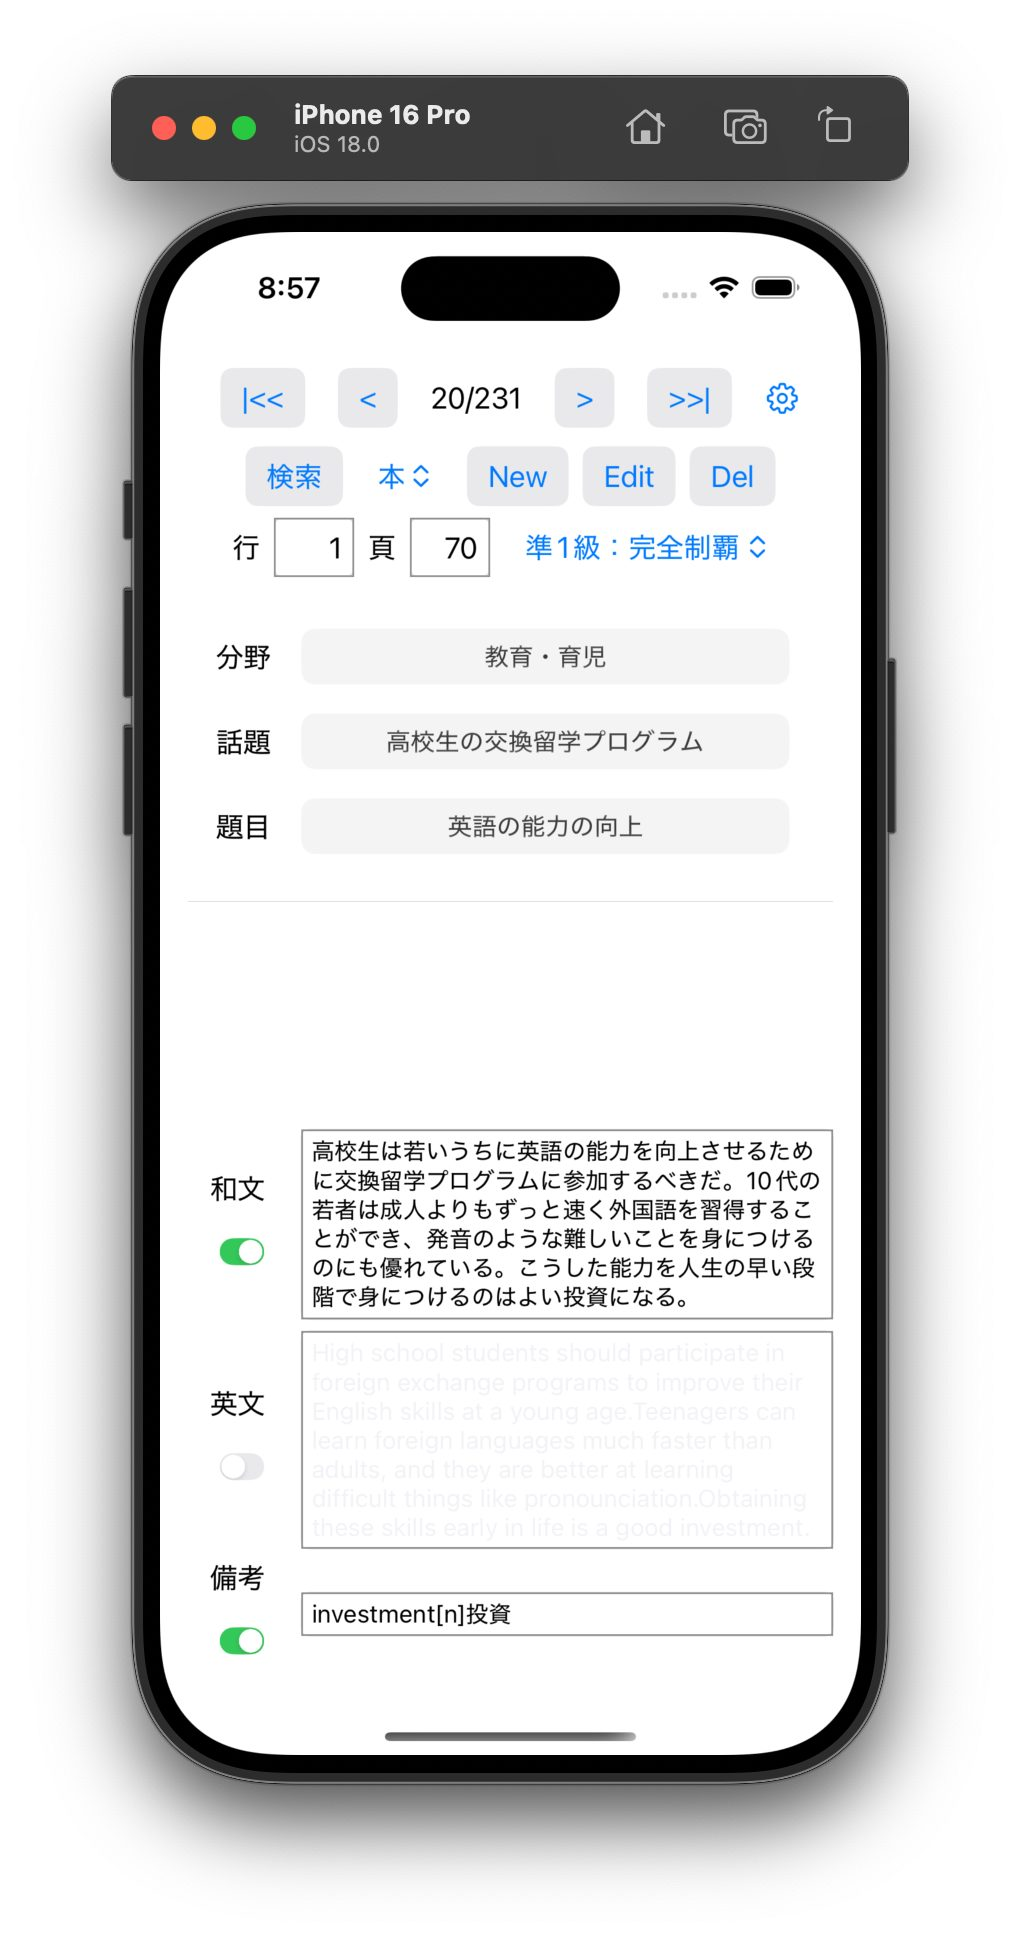
\includegraphics[width=\linewidth]{pictures/2024/10/20241016_091227_001.jpg}
\end{minipage}
\hfill
\begin{minipage}{0.48\linewidth}
\centering
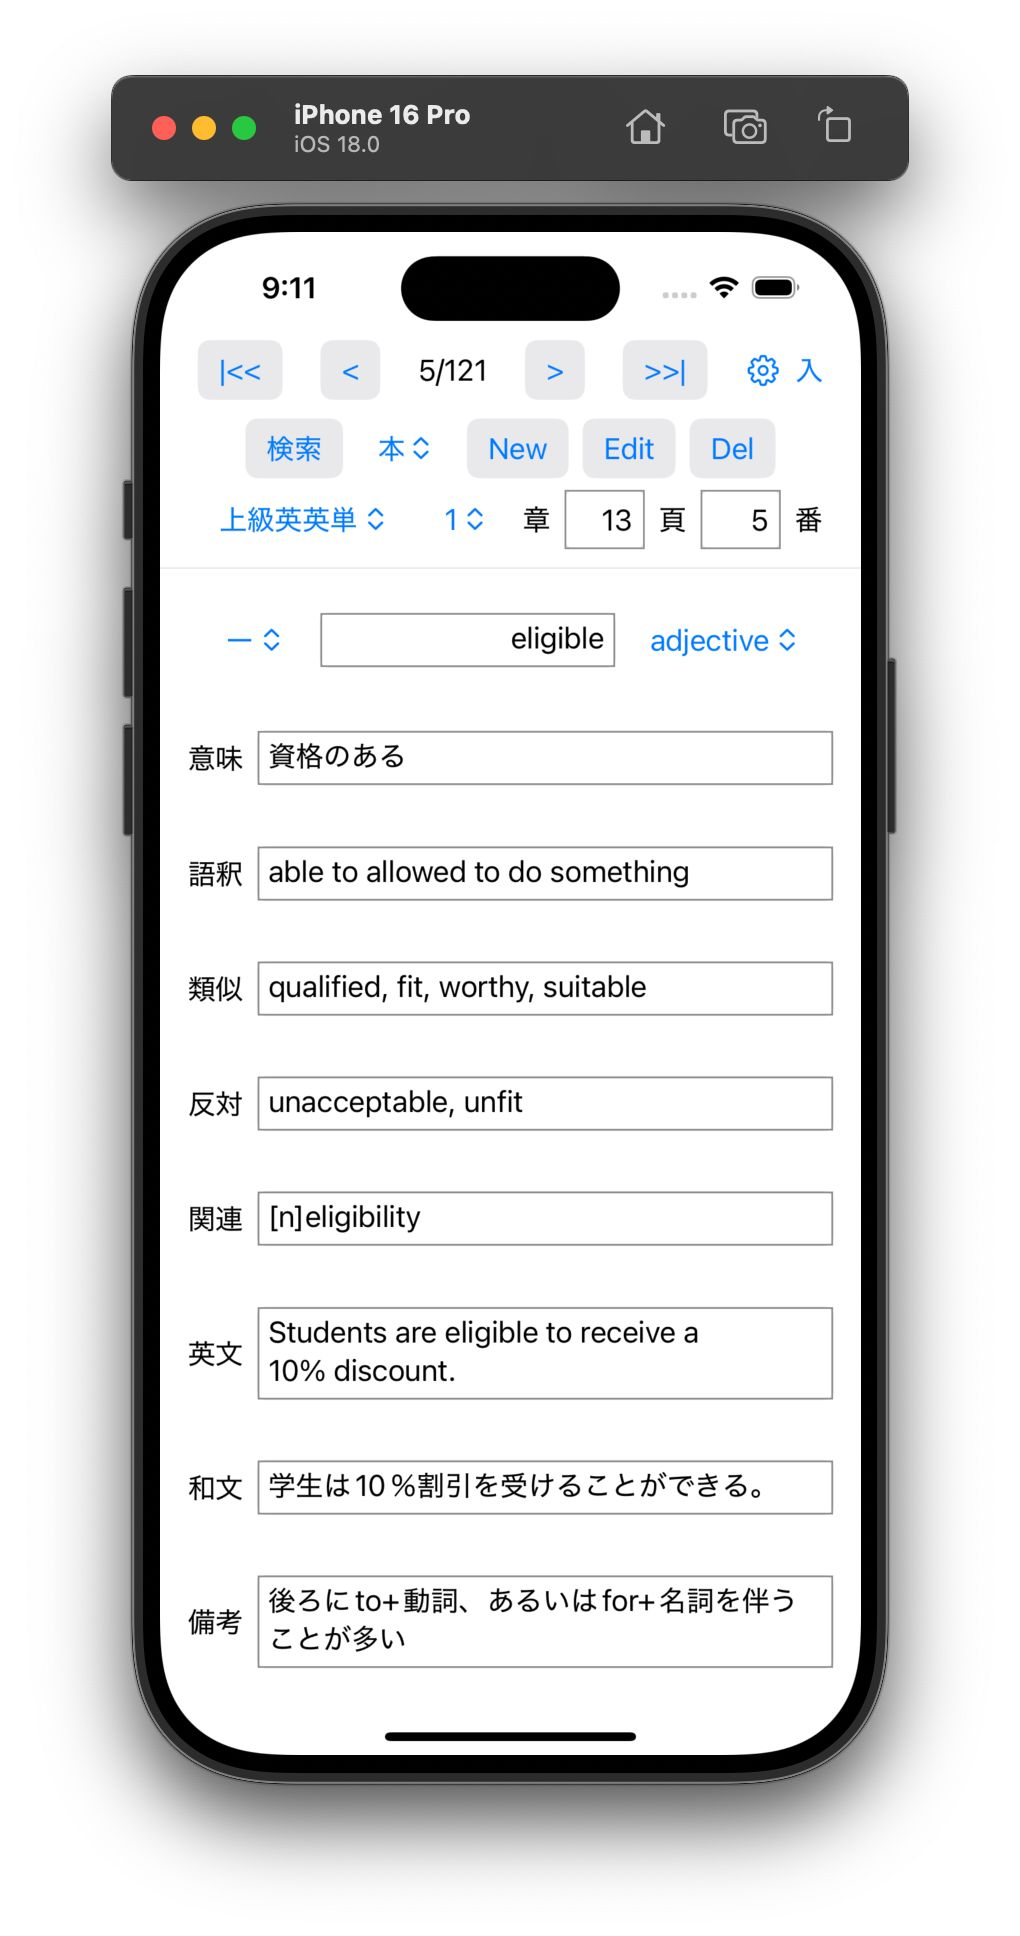
\includegraphics[width=\linewidth]{pictures/2024/10/20241016_091227_002.jpg}
\end{minipage}
\end{center}

\subsection*{2024年10月18日 22:34}
\addcontentsline{toc}{subsection}{2024年10月18日 22:34}

\paragraph{リンク}
\url{https://youtu.be/e71R60Sl9tg}

\begin{center}
\href{https://youtu.be/e71R60Sl9tg}{
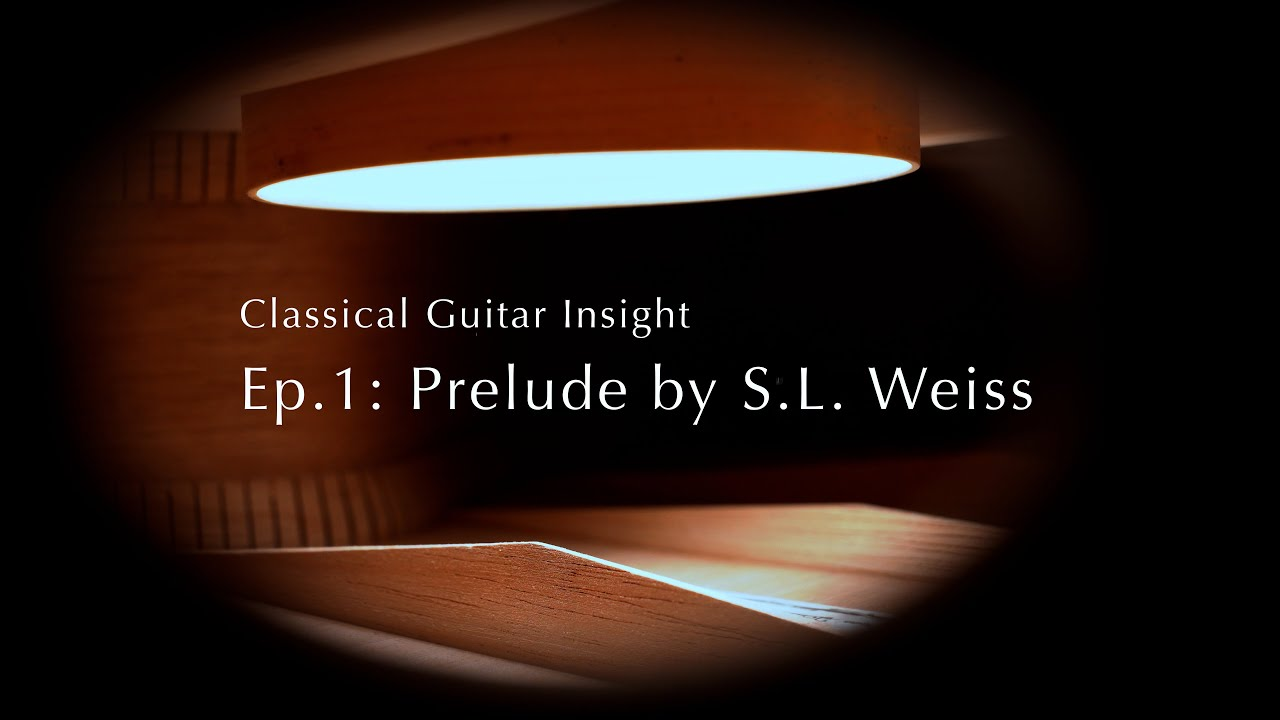
\includegraphics[width=0.48\linewidth]{pictures/youtube/2024/10/20241018_223439_youtube_001_e71R60Sl9tg.jpg}
}
\end{center}

\subsection*{2024年10月19日 14:06}
\addcontentsline{toc}{subsection}{2024年10月19日 14:06}

\url{https://www.facebook.com/share/p/3imC9322BwhibZmg/?mibextid=WC7FNe}




宴会とぶつかってしまい、第4回のライブでの受講はできませんでした。でも、ありがたい事に録画を受講できる様になっています。（いい時代になりました。便利になりました。）


(１) クヴァンツによる言葉の説明を、実際の楽譜の例で、しかも演奏付きで解説されていて、とても分かりやすい。言葉だけだったら読み解けないと思います。

(２) 前田方式による「装飾に使える音」が素晴らしい。そうだったのか、楽典を見直す必要ありますけど。何となく分かります。

(３) 移調によって、同じ曲が異なる曲想を持って鳴るだろうか。昔から疑問に思っていました。そもそも移調と言っても、音符を平行移動するだけの事ですし、或いは言うならば基準音の高さを変えただけですから。それで異なる曲想の表現ができた事になるものでしょうか。特に平均律なら何も変わらないはずなんじゃないか。でも、先生の演奏を聞くと、ずらしたどの調でもそれぞれいい雰囲気だと感じます。少なくとも、それぞれの調でそれぞれの曲想を持ち得る、それぞれの雰囲気になるんだなと感じました。

(４) 装飾の付け方で例示されていた楽譜で、13章の譜例への参照になっていたとは。この本を読み解くのが難しい訳だ。でも、強弱の例も含めて読み解くだけの根気は、私には残念ながらありません。

(５) カデンツの発展の歴史も興味深い内容でしたし、カデンツアの在り方みたいな話も、面白おかしく話されていて楽しく聞けました。


前田りり子先生には、是非とも「クヴァンツのフルート奏法を読み解く」というタイトルの本を著してほしいものです。クヴァンツの言葉だけでなく、譜例を入れて読み解いた、分かりやすいものを期待してしまいます。


＃前田りり子 \#トラヴェルソ \#Quantz \#クヴァンツ \#フルート奏法


⚪︎第一回目の聴講

\url{https://m.facebook.com/story.php?story_fbid=7876849065732519&id=100002225117991}




⚪︎第二回目の聴講

\url{https://m.facebook.com/story.php?story_fbid=1182866802781219&id=100031737316033}




⚪︎第三回目の聴講

\url{https://m.facebook.com/story.php?story_fbid=1182866802781219&id=100031737316033}



\subsection*{2024年10月22日 17:05}
\addcontentsline{toc}{subsection}{2024年10月22日 17:05}

\#iPhone のための \#英語学習アプリ の開発で行き詰まっていた「 \#Swift による \#CSV データの入出力」が、ようやく（何となく）完成した（みたいな）ので、最終的なclassにまとめている所です。本当はもう少し汎用性を持たせたい所が残ってはいるのですが、９割程度は満足できる形になっていると思います。


アプリの中では \#DB （\#SQLite3 ）で保持しているデータですが、DBをCSVの形で \#エクスポート できると共に、同じCSVから \#インポート してDBを再構築できる様になりました。これでようやく安心してデータの入力できますし、 \#iPad 上のアプリとiPhone上のアプリで、それぞれが入力したデータをCSVを介してやり取りする事で共有できるようになりました。


CSVデータの各レコードは改行で区切られており、それぞれのレコードはカンマでフィールドに分けられていて、特に文字列のフィールドはダブルクゥオートで挟んでいます。その様なCSVデータのフィールドの中に、(１)カンマがあっても、(２)ダブルクゥオートがあっても、(３)改行があっても、そのフィールドそのままに入出力できる様になった（みたいな）のです。（とても嬉しい）


当初はローカルルールを作って、フィールド内にダブルクゥオートやカンマや改行文字があったら、秘密の文字列に置き換えて出力しておいて、それを読み込む時に元に戻そうとしていました。しかし考えてみると、そんな事をしなくても通常通り出力したCSVデータは、 \#Excel や \#Numbers で正しく読めていました。という事は、そのままのデータを期待通りに解釈できる様なCSVデータ読み込みのコードは（力づくであったとしても）書ける「はず」だという気になりました。という訳で、あんなデータが来たらこうして、こんなデータが来たらああしてと、力任せのドロくさい（できれば見直したくない）コードですが、かなりのスッタモンダ試行錯誤の末に、ようやく出来上がった（様だ）という事なのです。


ついでながら、「 \#TextField では日本語入力に難あり」という問題についても、データを表示する時はTextFieldを使い、データを編集したり入力したりする時は、漢字入力Okの \#TextEdit の画面が現れる様にする事で解決しました。（めでたし、めでたし）


残りは、最後に学習していた場所を覚えておいて、次回立ち上げた時にその場所に戻る、そんな機能を持たせようかとも考えています。実はCSV入出力にとても満足していて、これで完成した様な気持ちになっています。


この投稿は、以下の記事の続きです

\url{https://m.facebook.com/story.php?story_fbid=8449971148420305&id=100002225117991}



\section{11月}

\subsection*{2024年11月01日 20:17}
\addcontentsline{toc}{subsection}{2024年11月01日 20:17}

\#Swift による \#英語学習アプリ の開発を「まだ」続けています。

今回は、 \#Apple watchと \#iPhone の連携に挑戦することにしました。

使い方は次の通り。\#Watch 上の \#単語カード のイメージです。


(１) 先ず、iPhone で学習する単語帳（本）を選択します。選んだ単語帳の中の全ての単語を選択状態にすることもできますが、その中の単語を章やページで絞り込む事もできます。

(２) 次に、iPhoneの右下の青いアイコンをタップして、Watchでの学習をスタートします（学習対象となる単語は、検索の結果絞り込んで得られた単語の一式です）

(３) すると、Watchに最初の単語が表示されますが、Watchの画面上を左にスワイプすると次の新しい単語が現れます。また右にスワイプすると一つ前の単語に表示が戻ります。


学習しようとする単語帳の１ページずつ（或いは１章ごと）に、iPhoneで学習対象の単語を絞り込んでは、Watchで（隙間時間に）学習するのがいいかもしれません。（受ケン生に使ってほしい所です）


添付は、ジャパンタイムズ社の「英語を英語で理解する英英英単語」の上級編からStage1の12ページの学習をしている所です。（ボタンの形や大きさ、色などを変えて色々遊んでみている）


※ WatchとiPhoneの通信のプログラムは、かなりデリケートな感じでとてもとても難しかったですよ。Watchは単語の1個ごとにiPhone と通信して、要求した単語データを受け取っては表示しています。また単語データの全体は、既に作成済みのiPhone上の英単語学習アプリで入力していたものを、 \#CSV を介して受け取り、ここでもやはり \#SQLite3 のDBに納めて使っています。なお、単語の日本語の意味の部分は、通常は見えていない様にしておいて、英単語をタップすると日本語が表示される様にしています（文字の透明度をトグルで変えてる）。ようやく完成してホッとしています。


今回の投稿は、以下の記事の続きです。

\url{https://m.facebook.com/story.php?story_fbid=8487420338008719&id=100002225117991}



\paragraph{写真}
\begin{center}
\begin{minipage}{0.48\linewidth}
\centering
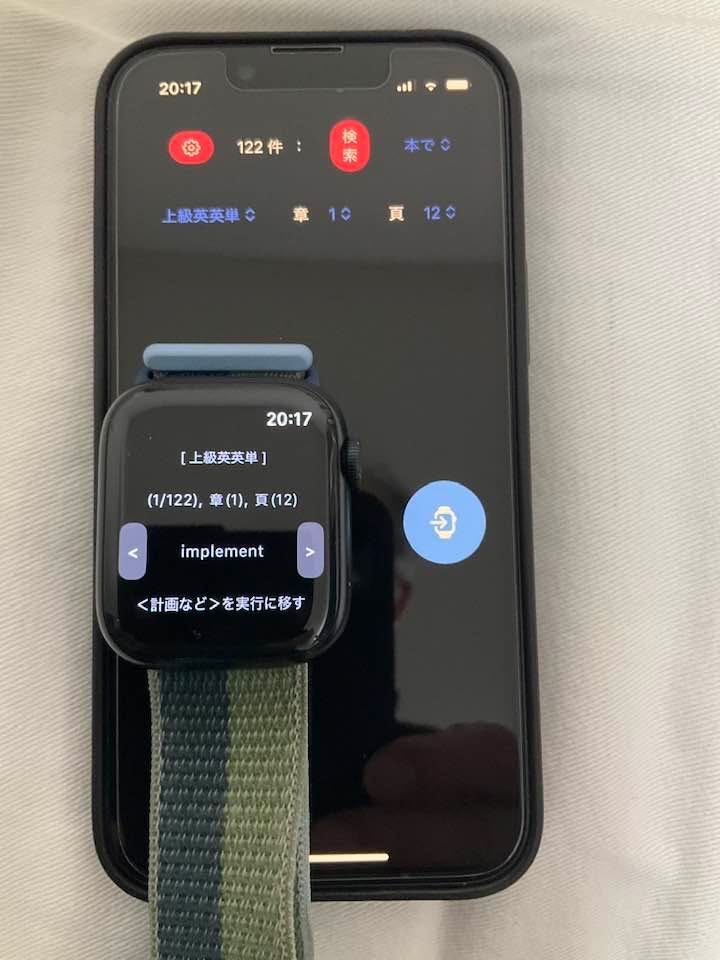
\includegraphics[width=\linewidth]{pictures/2024/11/20241101_201759_001.jpg}
\end{minipage}
\end{center}

\subsection*{2024年11月01日 22:00}
\addcontentsline{toc}{subsection}{2024年11月01日 22:00}

\url{https://m.facebook.com/story.php?story_fbid=1241669140234318&id=100031737316033}




＃前田りり子 \#トラヴェルソ \#Quantz \#クヴァンツ \#フルート奏法

\subsection*{2024年11月04日 17:34}
\addcontentsline{toc}{subsection}{2024年11月04日 17:34}

今日はよく歩いたよ。（9.5km=2時間43分）


\#犀川 縁を、（14:06） \#上菊橋 からスタートして、\#下菊橋 、 \#桜橋 、\#犀川大橋 、\#新橋 、\#御影橋 まで降りて行きました。御影橋はもう金沢駅前の道路に通じている橋だったのですね。帰りは \#長土塀 から、 \#尾山神社 の中を通って、 \#宮守坂 を登り、 \#金沢城 内を横切って \#石川門 に顔を出し、更に \#兼六園 の横の道を回り込んで、 \#石引 通りを歩いて戻りました（16:48）。有酸素運動しましたよ。（心拍数が高くなっているのは、おそらく宮守坂を登っている時だろうと思います。）

\paragraph{写真}
\begin{center}
\begin{minipage}{0.48\linewidth}
\centering
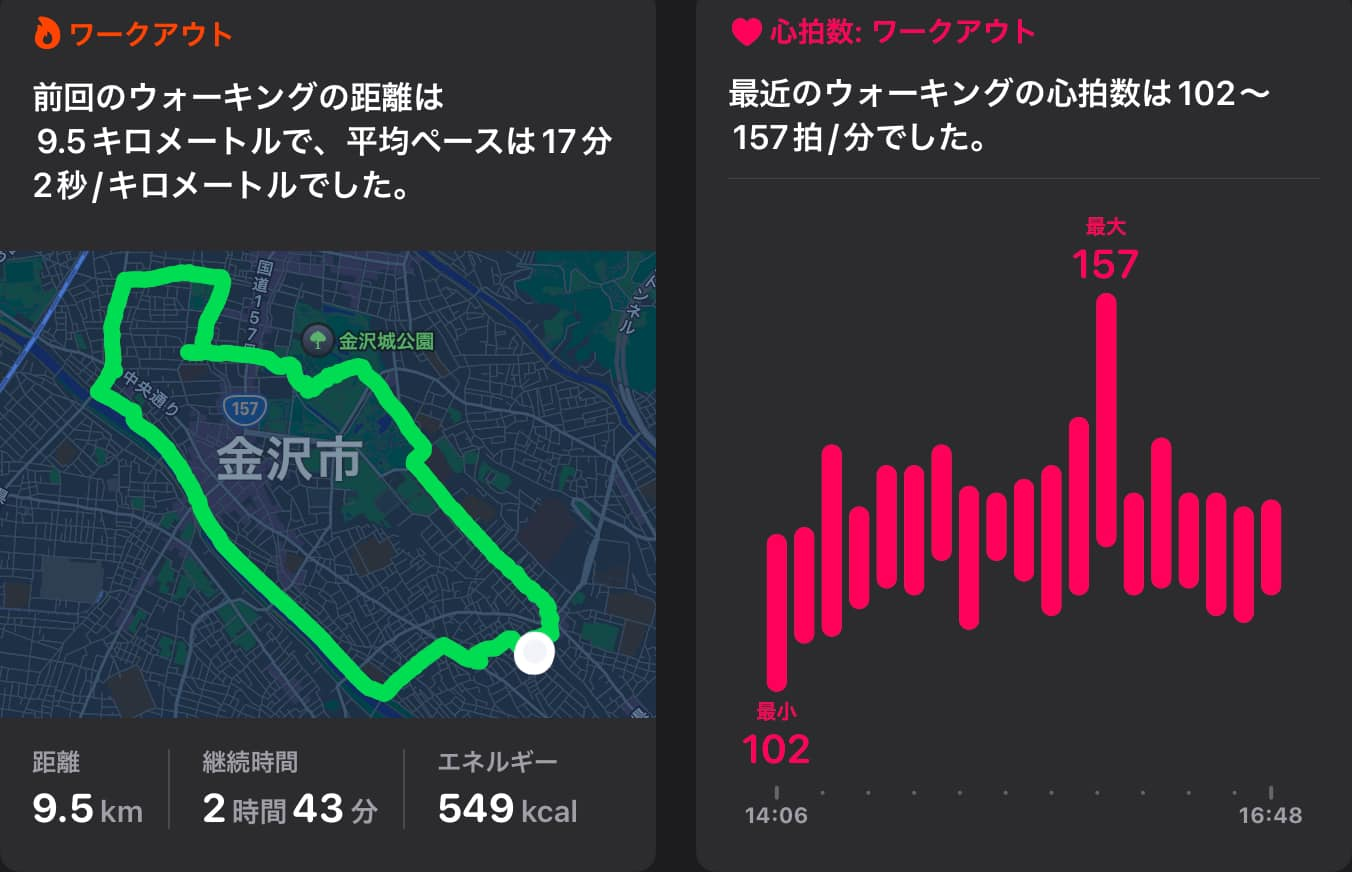
\includegraphics[width=\linewidth]{pictures/2024/11/20241104_173424_001.jpg}
\end{minipage}
\end{center}

\subsection*{2024年11月11日 18:22}
\addcontentsline{toc}{subsection}{2024年11月11日 18:22}

えー〜、嘘でしょう。眉唾でしょう、これは（表題しか読んでないけど）。（時間の進む方向も否定できる? ）最近は、量子もつれと言い、この事と言い、もう何でもありだな。（量子もつれはまだ量子の世界の話でしょうから、さもありなんと言う気もするが、熱力はマクロな世界に現れる現象でしょう。さて、どうなんだろう？早合点だったりしないか？）

\paragraph{リンク}
\url{https://www.itmedia.co.jp/news/articles/2411/11/news027.html}

\subsection*{2024年11月12日 00:12}
\addcontentsline{toc}{subsection}{2024年11月12日 00:12}

\url{https://m.facebook.com/story.php?story_fbid=1248609666206932&id=100031737316033}




豪華なメンバーだ。

演奏会には出かけられていないけど、 \#有田正広 先生のお元気そうな姿を見られて嬉しいよ。むかし、\#菅きよみ 先生に一度だけ指導を受けた事がある。その時、姿勢を良くする様に指摘を頂いた。「 \#バルト 先生は背筋がピンとしてた」と仰っていたけど、本当にそうなのがよく分かります。

\subsection*{2024年11月15日 09:04}
\addcontentsline{toc}{subsection}{2024年11月15日 09:04}

\#Adobe 、\#Microsoft 、\#Autodesk 各社のサブスクについて。


これまで、自作のテキストや資料、試験問題、或いは個人的な学習ノートなど、全んどのものを \#TeX + \#illustrator で書くようにしてきた。そこでは作図のために（個人的趣味に過ぎないのかもしれないが ）illustratorが便利だった。高価なんだけど個人的には使い慣れたillustrator以外は考えられず、Adobeのサブスクを購入してきた。でも \#TikZ （添付の翻訳本が出た）が登場したので、これでようやくillustratorのサブスクをやめられるか（どうか？）と期待して試している。


\url{https://www.overleaf.com/learn/latex/TikZ_package}




一方、\#Mac 付属の無料 \#Office アプリのおかげで、MicrosoftOfficeがサブスクを要求してきた頃には、MicrosoftOfficeは早々にアンインストールしてしまって、それ以来使っていません。（もうリタイアしているしね）


あと一つ心に引っかかっているのは、Autodesk社の \#AutoCAD  です。これも使えたらいいのですが。このサブスクが（Adobeと同様に）とても個人で購入しようと思える金額ではなく諦め状態です。以前描いたdrawingのデータがディスク内にあるのですが、現在はアプリが無くて開けません。そもそもAutoCadで2D図を描き、それを \#Fusion 360 に読み込んで3D化し、その3DモデルからNCデータを生成出力して、 \#NC 旋盤を動かすことをしていた。もうAutoCadが使えないと既存モデルの修正もできないよ。また3Dプリンタを使うこともあるので、Fusion 360で直接描いたデータもあれこれある。


AutoCadの（安価な）売り切りLite版（2次元機械製図特化でよい）for Mac があると嬉しいのですが（せめてFusion 360は何とか無料のまま使い続けられる事を願っています）。

\paragraph{写真}
\begin{center}
\begin{minipage}{0.48\linewidth}
\centering
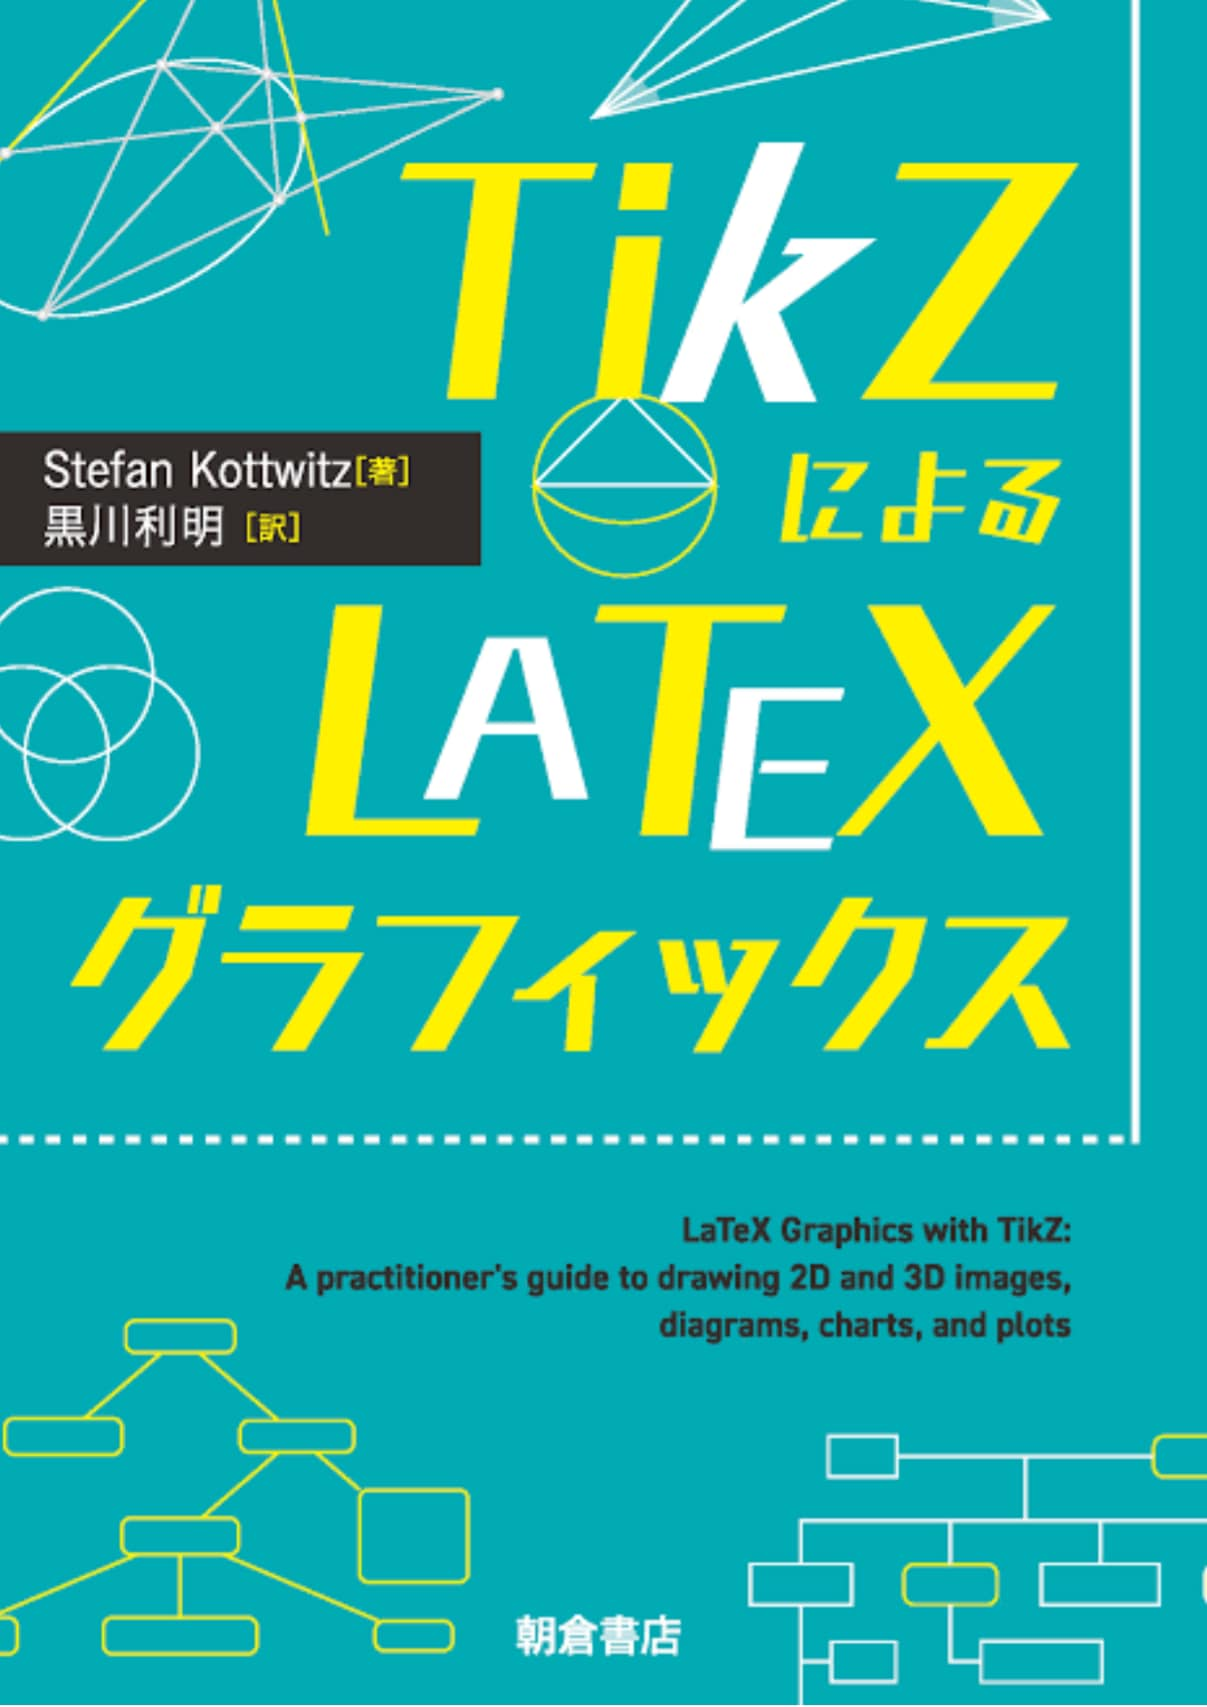
\includegraphics[width=\linewidth]{pictures/2024/11/20241115_090407_001.jpg}
\end{minipage}
\end{center}

\subsection*{2024年11月21日 00:33}
\addcontentsline{toc}{subsection}{2024年11月21日 00:33}

\paragraph{リンク}
\url{https://www.nhk.jp/p/ts/883N4WZPGQ/episode/te/8L7NWW599G/}

\subsection*{2024年11月23日 02:18}
\addcontentsline{toc}{subsection}{2024年11月23日 02:18}

「e： \#自然対数の底（＝船人は庭いっぱいに梯子置く）」だと思っていたが、いつの間にか「\#ネイピア数」という名前で呼ばれている。（Euler数って何だった？）

\subsection*{2024年11月26日 08:18}
\addcontentsline{toc}{subsection}{2024年11月26日 08:18}

2024年1月1日の \#地震 で崩壊した \#金沢城 の \#石垣 の修復工事の場面に遭遇した。城内数カ所で城壁の崩落が起きており、立ち入り禁止になっている。それぞれ修復が進められている様です。


この添付写真の場所は、陸軍の司令部が金沢城跡を利用していた際、弾薬庫？を本丸跡の手前あたりに置いていて、おそらくそことの物資搬入搬出の効率を考えて、元々あった城壁に穴を開けたということらしい。城内を歩きまわって注意深く城壁を見ていると、宮守坂の降り口など、何となく石が飛び出していて崩れるんじゃないかと心配になる様な場所もあります。（その様な周りは立ち入り禁止の柵が置かれています。）実は宮守坂も確か陸軍が作った坂だったんじゃなかったかな。（お城にあんな坂があったら、そこから攻めてきてくださいと言わんばかりだから、お城にはあり得ない出入り口になる坂ですから。）いずれの場所も陸軍の突貫工事だったのかもしれません。


添付の写真について、私の想像ですが、奥の方では、城壁を下から登って順に、そこの石が健全かどうか（浮いていないか、崩れ落ちそうではないか）といった調査が行われている様に見えました。また手前の方では、写真などの資料と見比べて、落ち着き場所の分かった石を見つけては、一つ一つ手前の方に並べていっていらっしゃる様に見えました。


金沢城では色んな年代の石垣の積み方を見る事ができますが、古い時代の石垣よりも、新しい時代の石垣の方が崩れているという話を耳にした事があります。

\paragraph{写真}
\begin{center}
\begin{minipage}{0.48\linewidth}
\centering
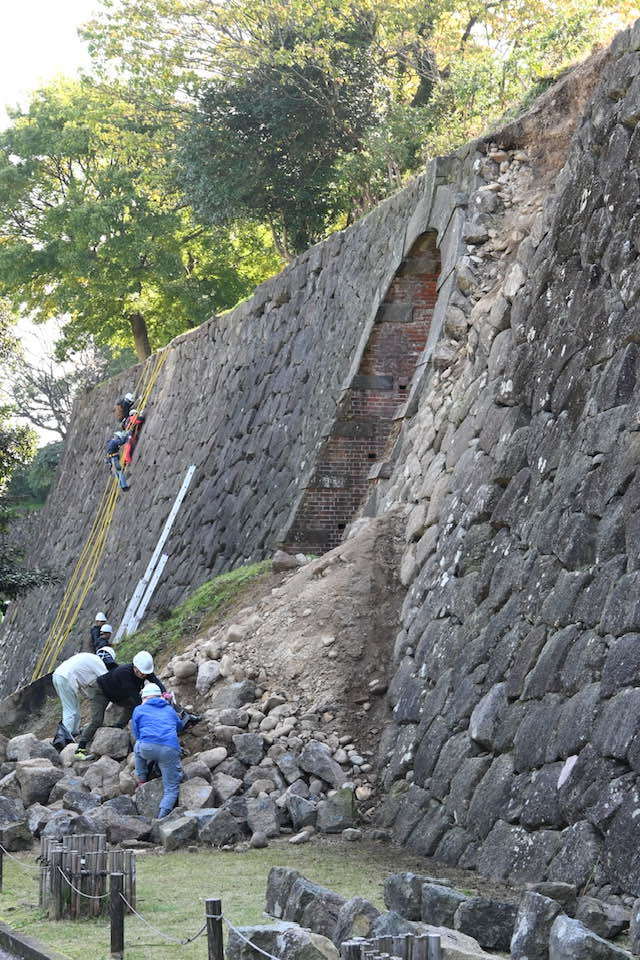
\includegraphics[width=\linewidth]{pictures/2024/11/20241126_081801_001.jpg}
\end{minipage}
\end{center}

\subsection*{2024年11月29日 19:34}
\addcontentsline{toc}{subsection}{2024年11月29日 19:34}

\paragraph{リンク}
\url{https://youtu.be/JGlFSHu3ieA}

\begin{center}
\href{https://youtu.be/JGlFSHu3ieA}{
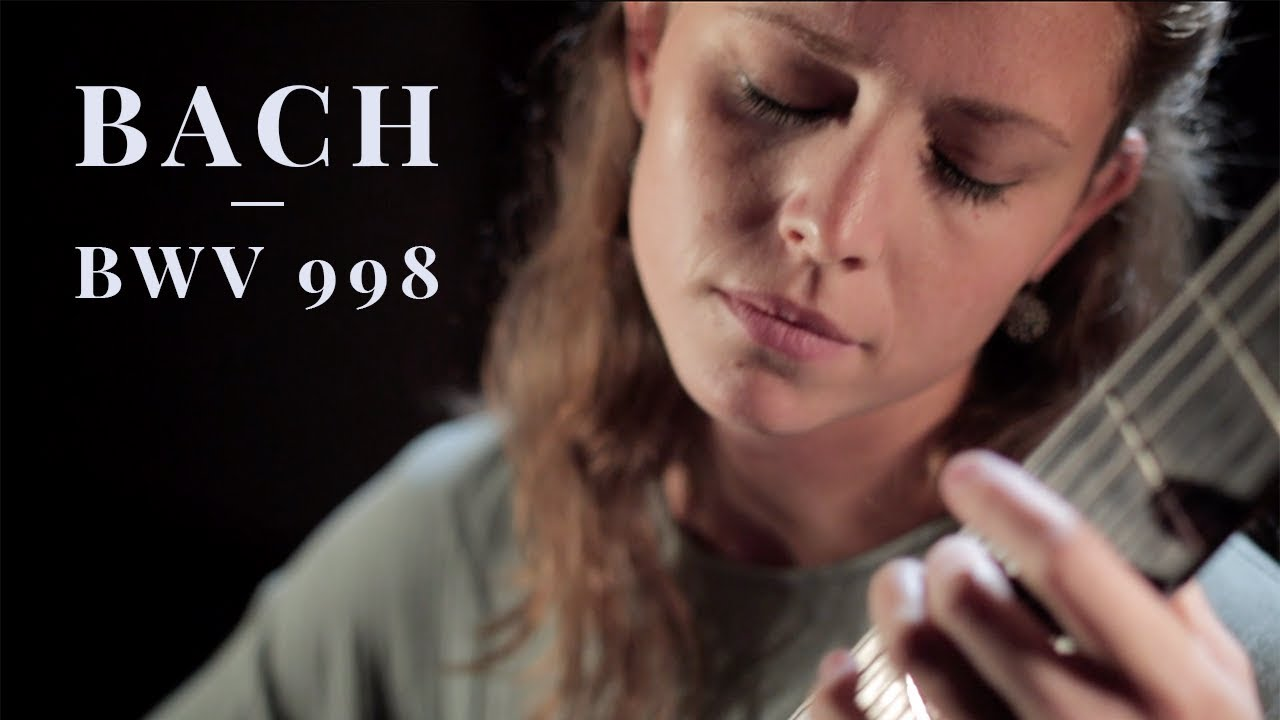
\includegraphics[width=0.48\linewidth]{pictures/youtube/2024/11/20241129_193435_youtube_001_JGlFSHu3ieA.jpg}
}
\end{center}

\section{12月}

\subsection*{2024年12月02日 06:25}
\addcontentsline{toc}{subsection}{2024年12月02日 06:25}

YouTube が「2024年のハイライト」と言うものを知らせてくれました。

\#BWV998 の \#Prelude ですが、この方（ \#山下愛陽 氏）の演奏を476分≒8時間聞いていたという事らしい。一回の再生が3分11秒ということなので、150回ほど聞いたことになるのかな。


実はこの曲、自分で演奏できる様になりたいと思って、最近練習をはじめました。最初は運指についてかなり悩みました。 \#セゴビア 編の楽譜ですが、色々納得のいかない部分（小指を伸ばさなくても開放弦ではダメなの？など）もありました。基本的に三度五度の和音を響かせる事を心がけて(弦をなるべく別にして）運指を決めていっています。しかし、二度の音程でも弦を別にして両方一緒に響かせた方が「たいそう趣がある≒唸りがあるとなお面白い」という気がしてきて、運指に迷ってしまいます（指も届かないし）。少しずつですが、自分なりの運指が固まってきつつあります。指板を見ながら演奏していて、「次何だっけ」と思って楽譜に目をやると、一体今楽譜のどこを演奏していたんだったか分からなくなっていて、途中中断してしまうこともしばしばです。最近になってようやく一通り通して（最後まで止まらずに）演奏？できる（≒音が出せる）様にはなってきましたが、ディナーミクやフレーズ、ボイスなど考える余裕はありません。ゆっくりのテンポ、落ち着いた雰囲気で曲を奏でられたら、と思っています。今は、毎日一回は通して弾いていこうと決めています。（ブランクを置くと、せっかく考えた運指を忘れてしまいそうですから。）tranquilloという指示も付いています。いつか気持ちよく弾き通せる日が来る事を信じて（願って）います。（が、、、どうでしょうか？）


\url{https://m.facebook.com/story.php?story_fbid=7819575471459879&id=100002225117991}



\paragraph{写真}
\begin{center}
\begin{minipage}{0.48\linewidth}
\centering
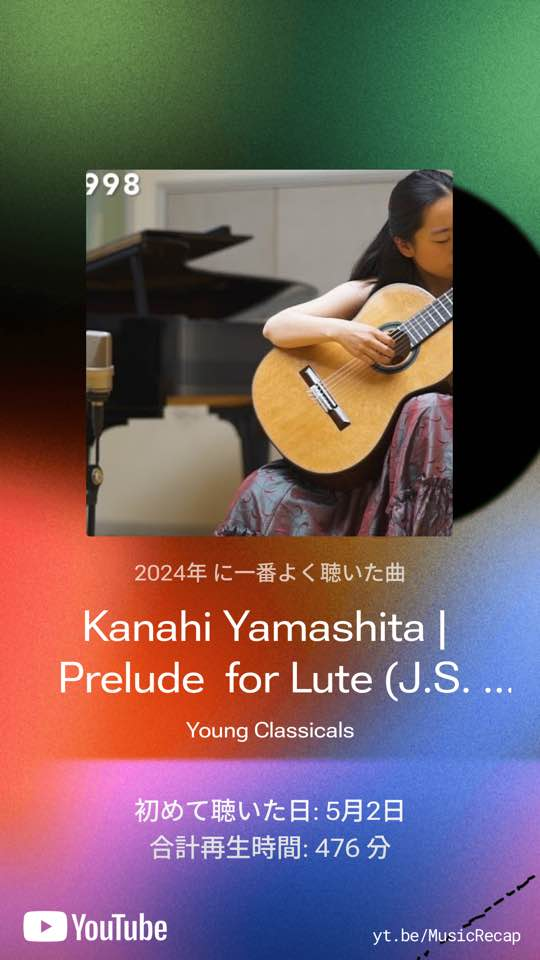
\includegraphics[width=\linewidth]{pictures/2024/12/20241202_062522_001.jpg}
\end{minipage}
\end{center}

\subsection*{2024年12月10日 17:56}
\addcontentsline{toc}{subsection}{2024年12月10日 17:56}

\url{https://corp.oup.com/news/brain-rot-named-oxford-word-of-the-year-2024/}




2024年の新語（oxford word of the year 2024）‘Brain rot’[noun]


‘Brain rot’ is defined as “the supposed deterioration of a person’s mental or intellectual state, especially viewed as the result of overconsumption of material (now particularly online content) considered to be trivial or unchallenging. Also: something characterized as likely to lead to such deterioration”.


「とりわけ、オンライン.コンテンツ」の過剰消費の結果として、、(\textasciicircum{}\textasciicircum{};💦

\paragraph{写真}
\begin{center}
\begin{minipage}{0.48\linewidth}
\centering
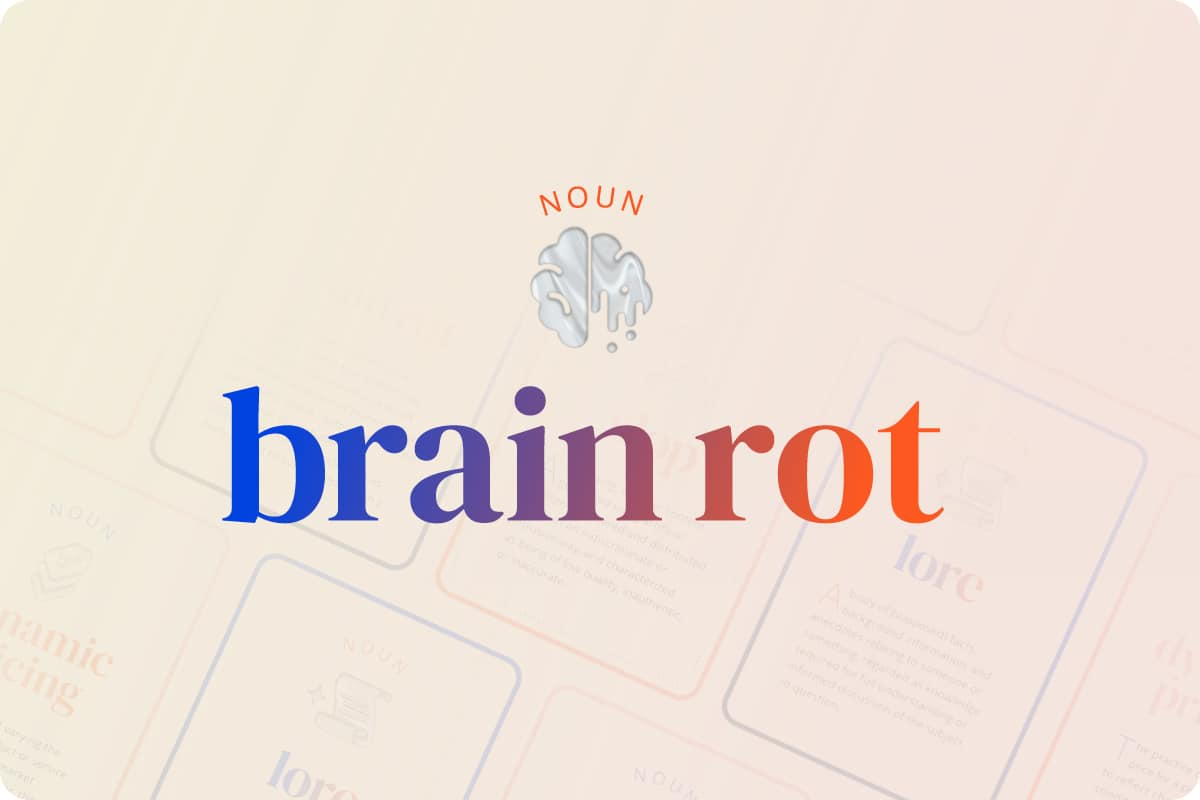
\includegraphics[width=\linewidth]{pictures/2024/12/20241210_175650_001.jpg}
\end{minipage}
\end{center}

\subsection*{2024年12月11日 09:26}
\addcontentsline{toc}{subsection}{2024年12月11日 09:26}

\url{https://x.com/gustavodudamel/status/1866550031202852928}




G.FaureのRequiemからPie Jesu。

天使の歌声（復興なったノートルダム大聖堂）

\paragraph{写真}
\begin{center}
\begin{minipage}{0.48\linewidth}
\centering
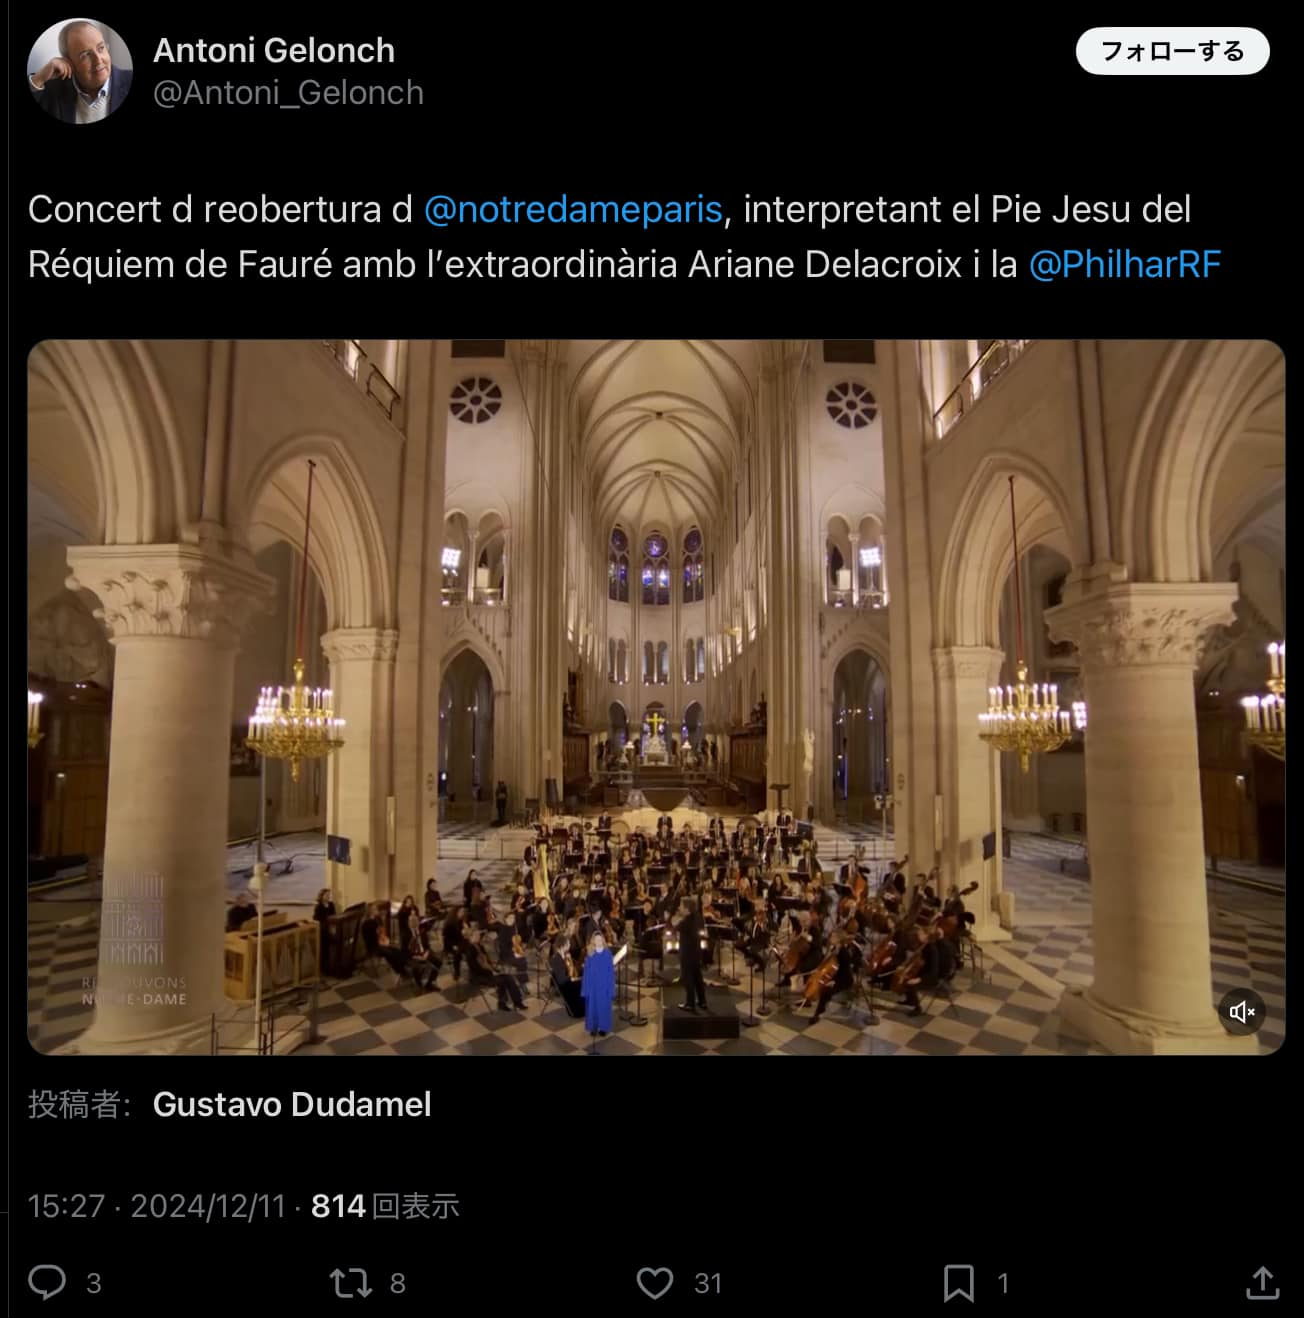
\includegraphics[width=\linewidth]{pictures/2024/12/20241211_092621_001.jpg}
\end{minipage}
\end{center}

\subsection*{2024年12月12日 12:46}
\addcontentsline{toc}{subsection}{2024年12月12日 12:46}

\paragraph{リンク}
\url{https://x.com/jump_213_ei/status/1866878210060980366?s=12&t=5VtsOkpki6juEjPXsBq8hg}

\subsection*{2024年12月13日 10:01}
\addcontentsline{toc}{subsection}{2024年12月13日 10:01}

\paragraph{リンク}
\url{https://journals.aps.org/prxquantum/abstract/10.1103/PRXQuantum.5.030355}

\subsection*{2024年12月13日 11:56}
\addcontentsline{toc}{subsection}{2024年12月13日 11:56}

\paragraph{リンク}
\url{https://journals.aps.org/prl/abstract/10.1103/PhysRevLett.133.137101}

\subsection*{2024年12月13日 22:30}
\addcontentsline{toc}{subsection}{2024年12月13日 22:30}

\paragraph{リンク}
\url{https://youtu.be/zaF0vu_AMSo}

\begin{center}
\href{https://youtu.be/zaF0vu_AMSo}{
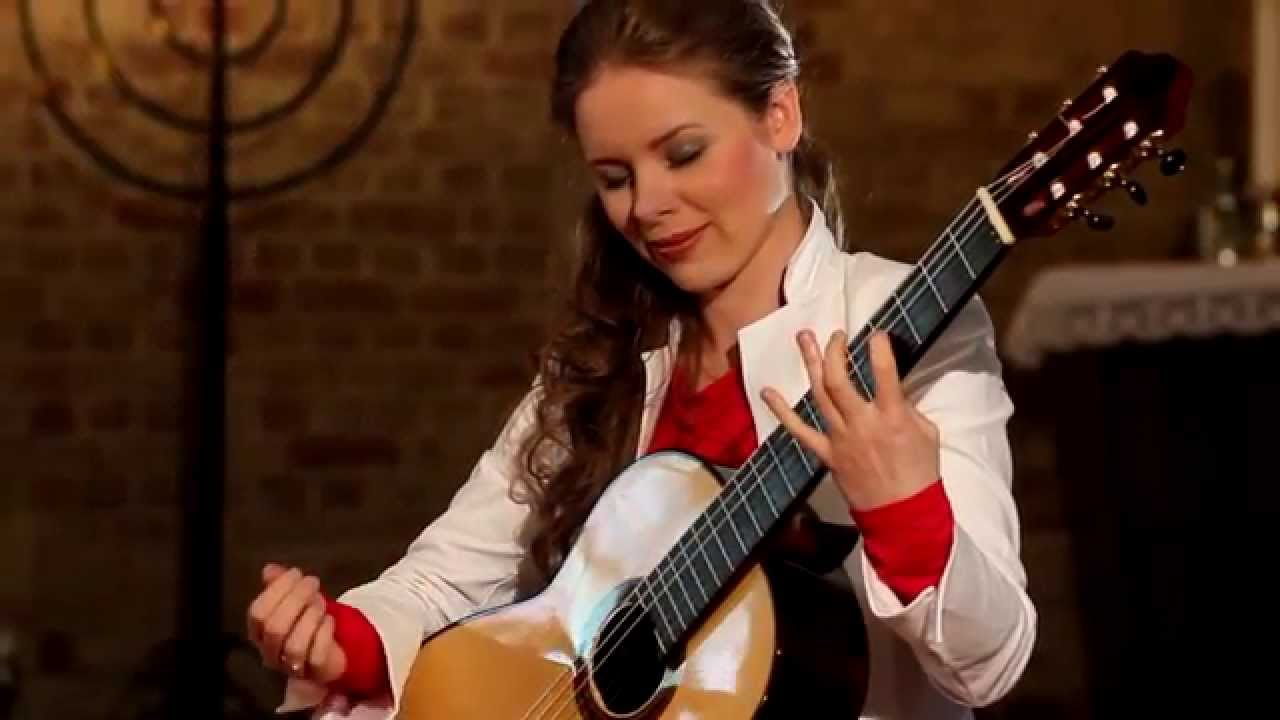
\includegraphics[width=0.48\linewidth]{pictures/youtube/2024/12/20241213_223035_youtube_001_zaF0vu_AMSo.jpg}
}
\end{center}

\subsection*{2024年12月13日 23:47}
\addcontentsline{toc}{subsection}{2024年12月13日 23:47}

\url{https://m.facebook.com/story.php?story_fbid=1270390147362217&id=100031737316033}



\subsection*{2024年12月14日 13:01}
\addcontentsline{toc}{subsection}{2024年12月14日 13:01}

\paragraph{リンク}
\url{https://youtu.be/YhFJLyfQpn4}

\begin{center}
\href{https://youtu.be/YhFJLyfQpn4}{
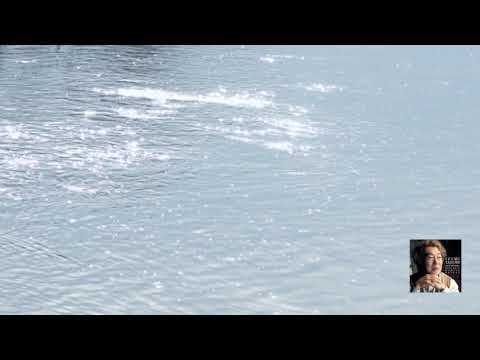
\includegraphics[width=0.48\linewidth]{pictures/youtube/2024/12/20241214_130123_youtube_001_YhFJLyfQpn4.jpg}
}
\end{center}

\subsection*{2024年12月14日 14:04}
\addcontentsline{toc}{subsection}{2024年12月14日 14:04}

\url{https://youtu.be/TH9lvz178UA}

\begin{center}
\href{https://youtu.be/TH9lvz178UA}{

\includegraphics[width=0.48\linewidth]{pictures/youtube/2024/12/20241214_140416_youtube_001_TH9lvz178UA.jpg}
}
\end{center}



\subsection*{2024年12月17日 18:21}
\addcontentsline{toc}{subsection}{2024年12月17日 18:21}

\url{https://youtu.be/axow9KtAvsk}

\begin{center}
\href{https://youtu.be/axow9KtAvsk}{
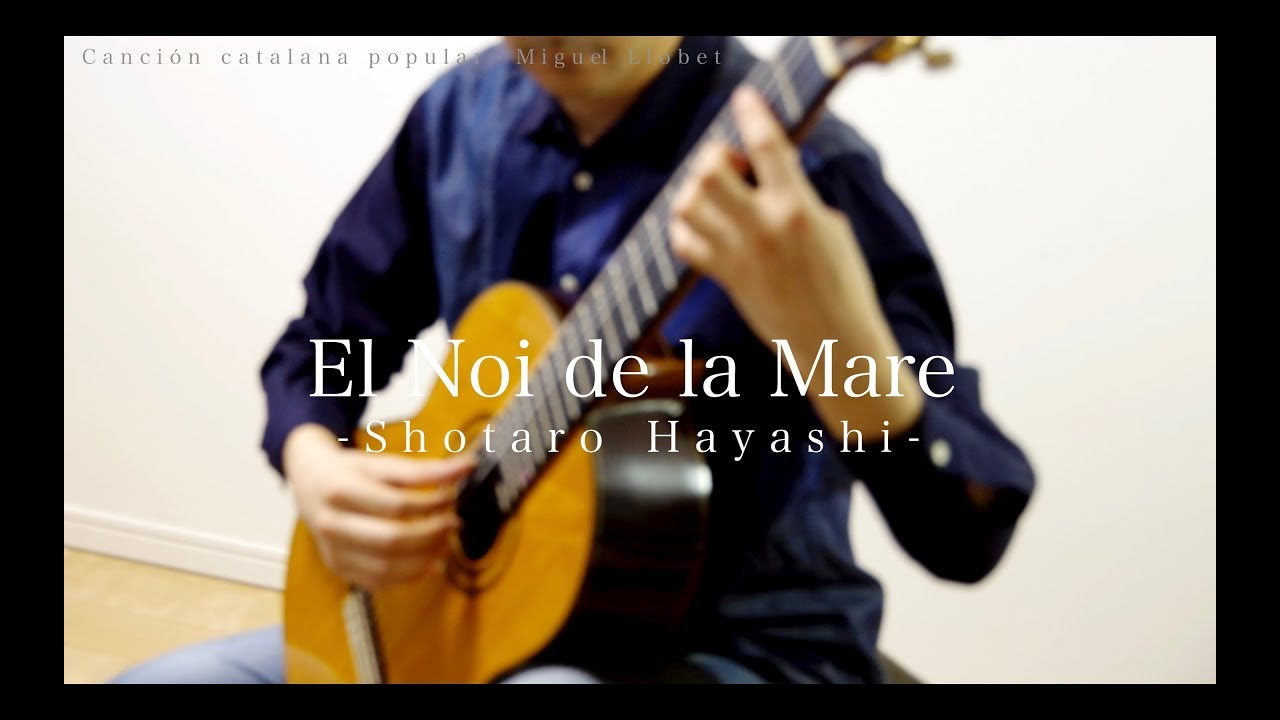
\includegraphics[width=0.48\linewidth]{pictures/youtube/2024/12/20241217_182154_youtube_001_axow9KtAvsk.jpg}
}
\end{center}




\#カタロニア民謡 の「 \#聖母の御子 」はいろいろな楽器で演奏されている様です。ギター編でも複数の編曲版（\#セゴビア編、フェレール編、カーノ編、\#ポンセ編 など）があるみたいなのですが、個人的には \#リョベート編 を攻略したいと考えています。添付は \#林祥太郎 氏のリョベート編による演奏です。美しい和音の響きが流れますし、非和声音の部分なのか（知らんけど）経過音の所なんかの独特の音が良いですね。そしてクリスマス🎄の雰囲気を醸してくれるハーモニクスによる演奏箇所もあって魅力的です。


この方（

\url{https://youtu.be/KkS7MYUS3Wk}

\begin{center}
\href{https://youtu.be/KkS7MYUS3Wk}{
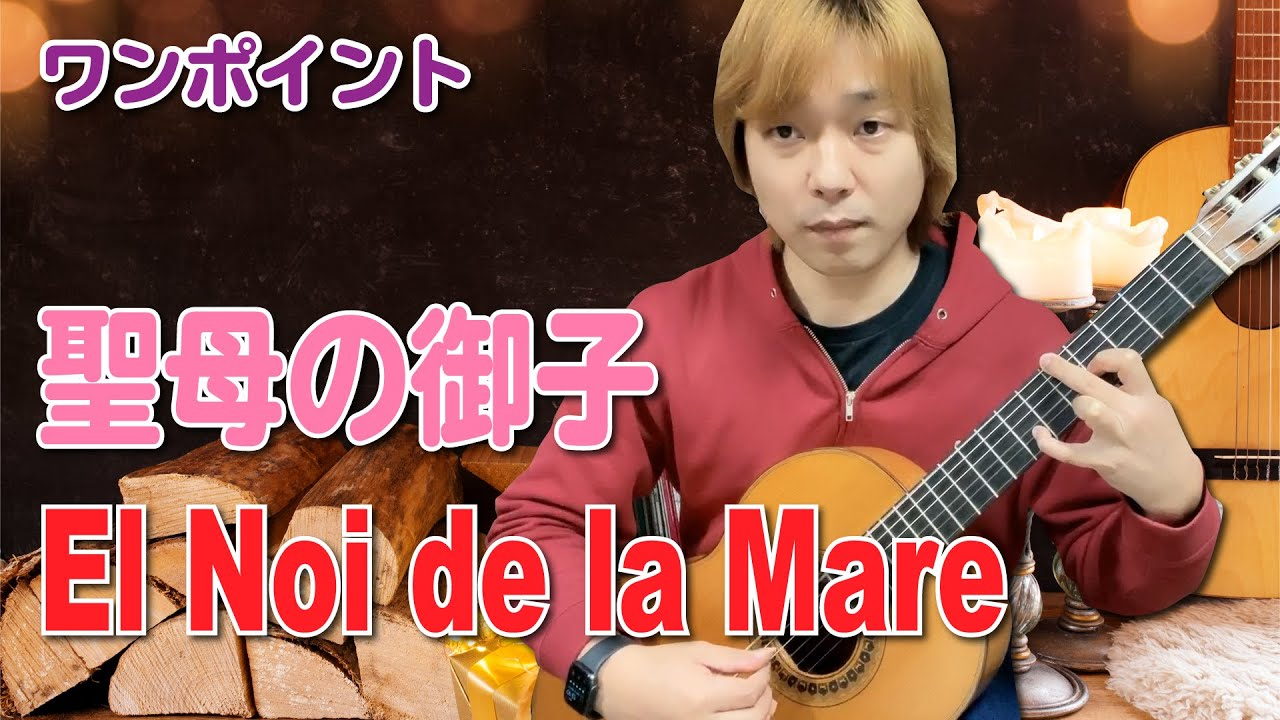
\includegraphics[width=0.48\linewidth]{pictures/youtube/2024/12/20241217_182154_youtube_002_KkS7MYUS3Wk.jpg}
}
\end{center}

）もおっしゃっている通り、指のストレッチが必要になる所が複数ヶ所ある。その内の特に一ヶ所は「無理かも」と思うくらい厳しい指の形なので、パッと押さえられない。また、音を残して繋ぎたい所がそこかしこにあるのですが、これもまた指をストレッチして、更に素早く次にくる和音を押さえないと残せない。テンポはゆっくりですし、そもそも曲自体も短い事ですから、何とかならないものかと奮闘してみています。（それにしても途切れ途切れになってしまう\textasciicircum{}\textasciicircum{};）


（その後の追伸）最も困難な運指の所ですが、３弦のBの音（４フレット目にある）は諦めて、５フレットのセーハ（６弦のG＋１弦のA）＋７フレット２弦のFis でよしとする事にしてみたのだけど。


（さらにその後）諦めていた３弦のBも含めて、少し無理すれば何とか押さえられる様になってきた。

\subsection*{2024年12月17日 18:22}
\addcontentsline{toc}{subsection}{2024年12月17日 18:22}

\paragraph{リンク}
\url{https://youtu.be/axow9KtAvsk}

\begin{center}
\href{https://youtu.be/axow9KtAvsk}{
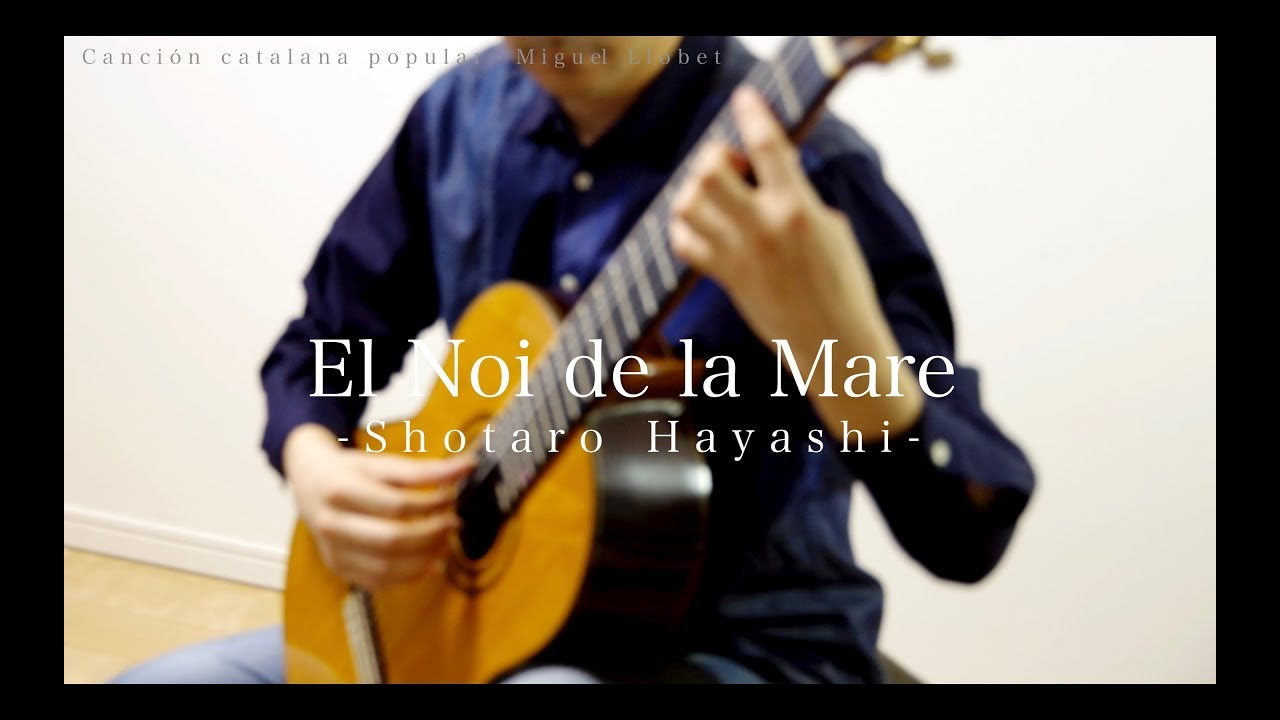
\includegraphics[width=0.48\linewidth]{pictures/youtube/2024/12/20241217_182251_youtube_001_axow9KtAvsk.jpg}
}
\end{center}

\subsection*{2024年12月17日 20:16}
\addcontentsline{toc}{subsection}{2024年12月17日 20:16}

\paragraph{リンク}
\url{https://x.com/yukasekiguchi57/status/1867804994986270883}

\subsection*{2024年12月18日 08:47}
\addcontentsline{toc}{subsection}{2024年12月18日 08:47}

\paragraph{リンク}
\url{https://youtu.be/Pb1MNUoJg6c}

\begin{center}
\href{https://youtu.be/Pb1MNUoJg6c}{
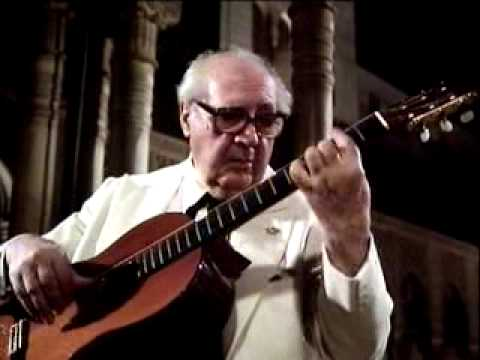
\includegraphics[width=0.48\linewidth]{pictures/youtube/2024/12/20241218_084703_youtube_001_Pb1MNUoJg6c.jpg}
}
\end{center}

\subsection*{2024年12月19日 01:00}
\addcontentsline{toc}{subsection}{2024年12月19日 01:00}

\paragraph{リンク}
\url{https://youtu.be/Eonr9sOswi8}

\begin{center}
\href{https://youtu.be/Eonr9sOswi8}{
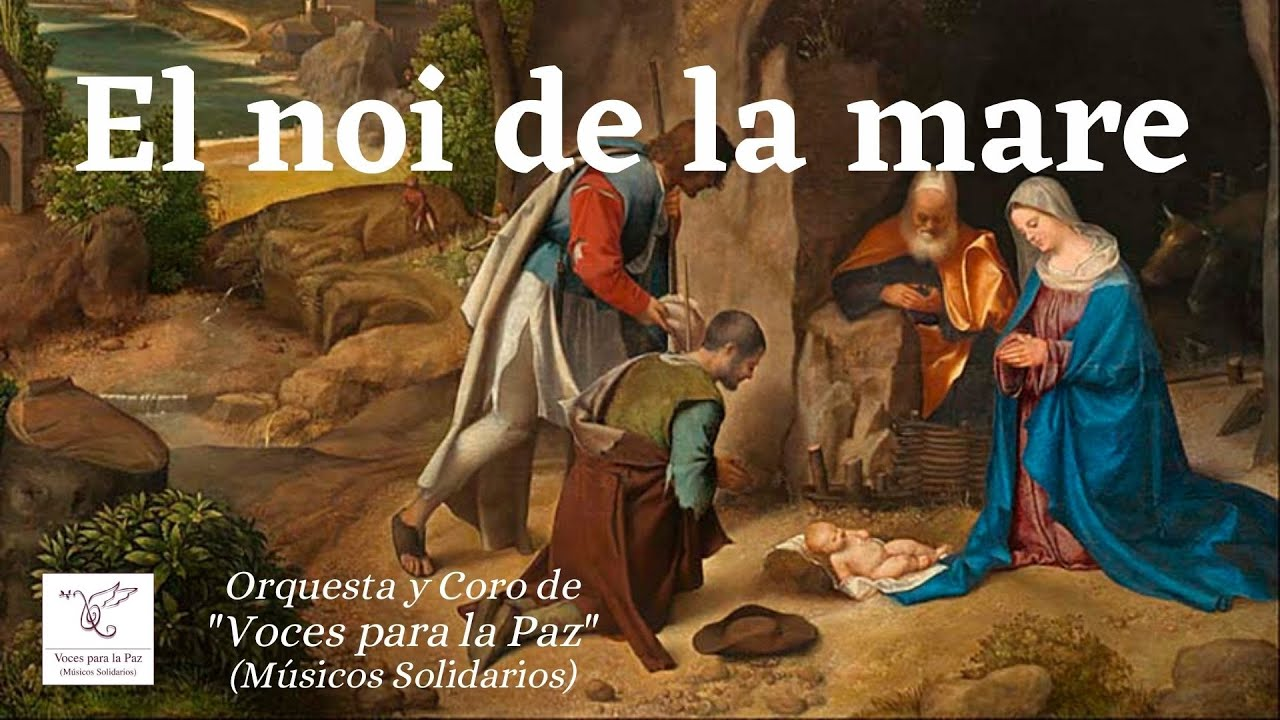
\includegraphics[width=0.48\linewidth]{pictures/youtube/2024/12/20241219_010051_youtube_001_Eonr9sOswi8.jpg}
}
\end{center}

\subsection*{2024年12月19日 19:53}
\addcontentsline{toc}{subsection}{2024年12月19日 19:53}

\paragraph{リンク}
\url{https://youtu.be/dUzD6UrscWw}

\begin{center}
\href{https://youtu.be/dUzD6UrscWw}{
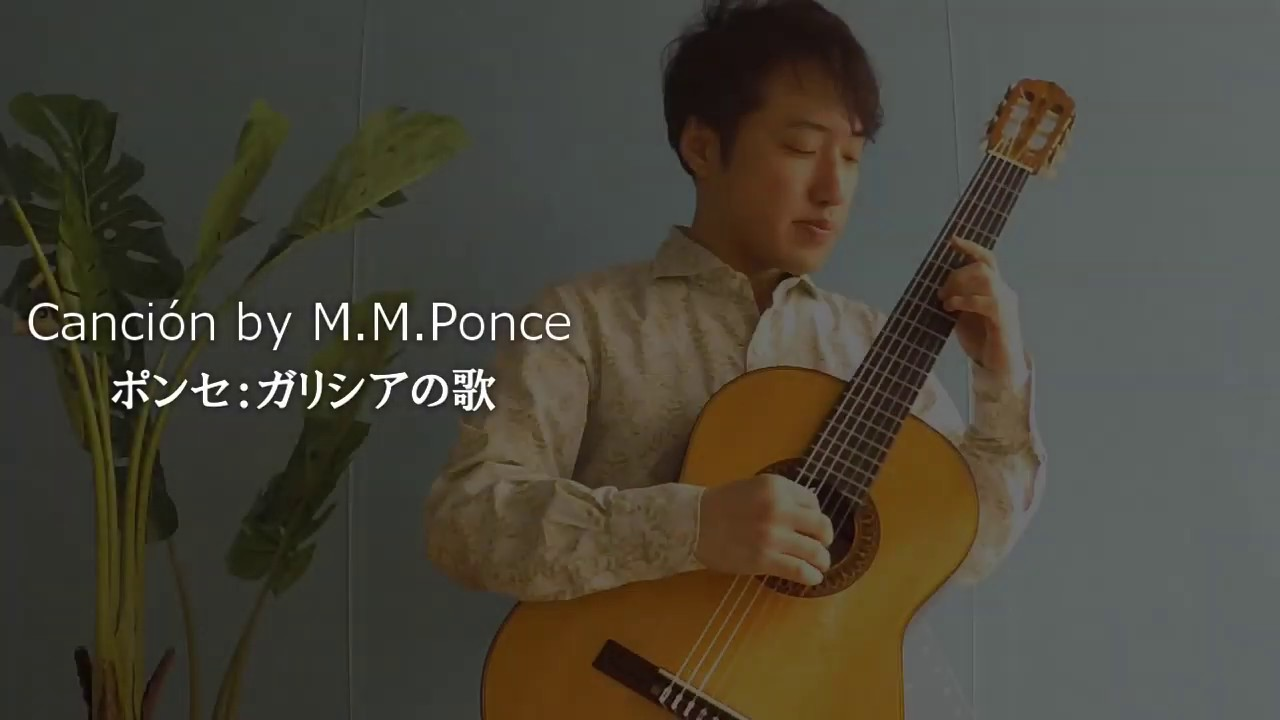
\includegraphics[width=0.48\linewidth]{pictures/youtube/2024/12/20241219_195327_youtube_001_dUzD6UrscWw.jpg}
}
\end{center}

\subsection*{2024年12月21日 19:48}
\addcontentsline{toc}{subsection}{2024年12月21日 19:48}

\paragraph{リンク}
\url{https://doi.org/10.1103/PhysRevA.109.052212?_gl=1\%2A18uxv70\%2A_gcl_au\%2AMTQ1MjgyNDczMS4xNzMyNjY0MTEx\%2A_ga\%2ANDc0MDg5NTkwLjE3MjAzOTI3NTM.\%2A_ga_ZS5V2B2DR1\%2AMTczNDc2MzAwMS40OS4wLjE3MzQ3NjMwMDEuNjAuMC4xMzczODYwMjk2}

\subsection*{2024年12月22日 05:34}
\addcontentsline{toc}{subsection}{2024年12月22日 05:34}

気になっている。12月28日22:00から \#NHK総合 で放送される「\#NHKスペシャル『\#量子もつれ \#アインシュタイン 最後の謎』」


NHKは凄い。どんな視聴者を想定しているんだろうか。

私の様に「光の速さ（有限）を超える情報伝達手段はない」と思って来た凡人にとって、「量子もつれ」はにわかには信じられない事です。（きっと私の様な常人を対象に想定しているのだと思います。）この番組によって、手軽に「なるほど」と思えたら、それにこしたことはないのですけど。（Electricityという曲も聞いた事ないし、楽しみです😊）


\url{https://www.nhk.jp/p/special/ts/2NY2QQLPM3/episode/te/BX6PWY3N59/}



\paragraph{リンク}
\url{https://natalie.mu/music/news/604418}

\subsection*{2024年12月23日 01:36}
\addcontentsline{toc}{subsection}{2024年12月23日 01:36}

\url{https://youtu.be/2MOTNxNYwdM}

\begin{center}
\href{https://youtu.be/2MOTNxNYwdM}{
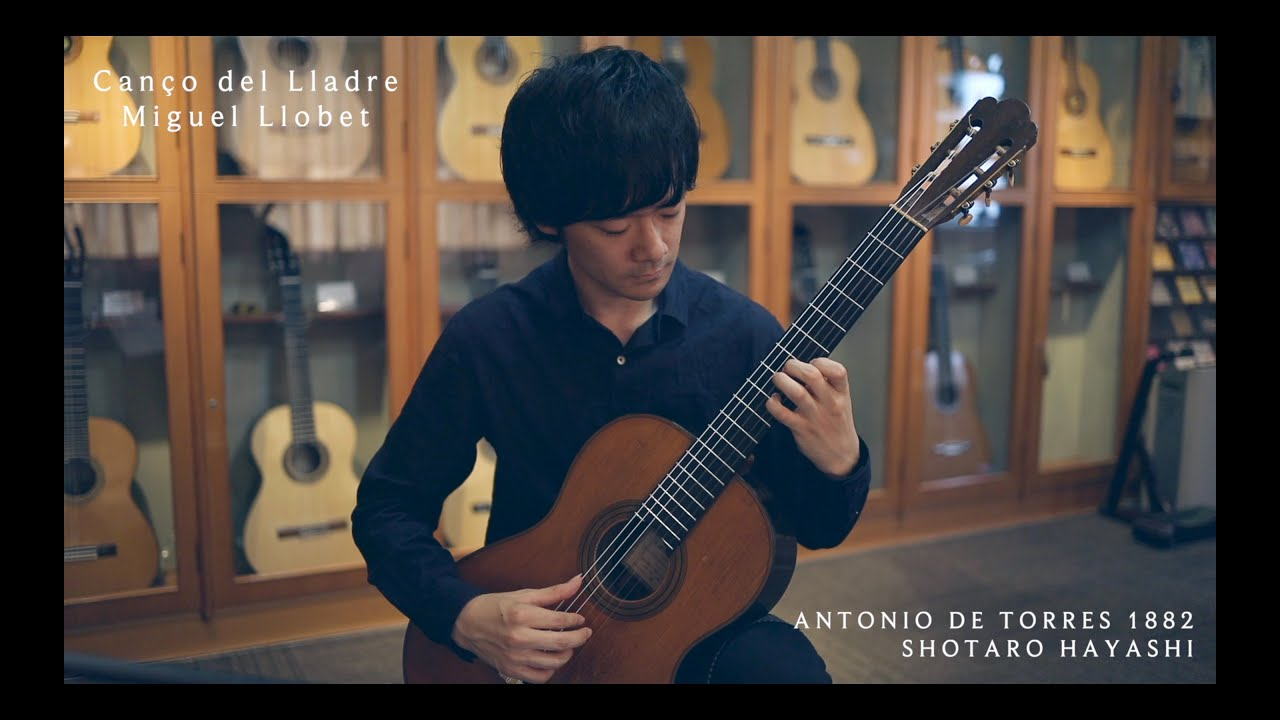
\includegraphics[width=0.48\linewidth]{pictures/youtube/2024/12/20241223_013624_youtube_001_2MOTNxNYwdM.jpg}
}
\end{center}




聖母の御子に続く \#カタロニア民謡 シリーズ、\#盗賊の歌 です。添付は \#林祥太郎 氏による \#リョベート編 の演奏です。


クラシックギターのレパートリーとしてポピュラーなこの曲は、先ずはテンポ・ルバート、そしてリョベート編らしいハーモニクスやグリッサンド（ポルタメント）という辺りが魅力的に聞こえる曲だと思います。これらはギターの独奏であればこその表現ではあるのですが、過度のルバートや大げさなポルタメントの多用は、（とりわけ現代においては）悪趣味と言わざるを得ません。古賀政男サウンドになってしまうと、それはまた違う世界の話ですし。演奏にあたってはメタな視点に立った、ある程度のストイックさが求められるのかもしれません。その点、林祥太郎氏の演奏はさすがです。趣味の良さ、冷静さを感じます。その一方で、楽器の音色にも起因しているのか、ロマチックな雰囲気も表現されています。


演奏に使われている楽器の作者は、アントニオ・デ・トーレス。スペイン・アルメリア出身のギター製作家。現在製作されているクラシック・ギターの原型となるギターを製作した方らしい。（フルートの世界では、ドイツのテオバルト・ベームが似た様な役割を果たしている。ベームは、従来のフルートの楽器としての性能を向上させた「ベーム式フルート」を完成させている。また、トーレスとベームは同じ時代を生きていた様だ。）


聖母の御子を攻略したら、そのうち盗賊の歌にも挑戦してみたいのですが、ハーモニクスとハイポジションの運指が難しそうだ。

\subsection*{2024年12月26日 01:31}
\addcontentsline{toc}{subsection}{2024年12月26日 01:31}

\url{https://nazology.kusuguru.co.jp/archives/167844}



\subsection*{2024年12月26日 01:37}
\addcontentsline{toc}{subsection}{2024年12月26日 01:37}

\paragraph{リンク}
\url{https://journals.aps.org/pra/abstract/10.1103/PhysRevA.109.052212}

\subsection*{2024年12月26日 15:21}
\addcontentsline{toc}{subsection}{2024年12月26日 15:21}

\url{https://www.nhk.jp/p/ts/883N4WZPGQ/episode/te/8L7NWW599G/?fbclid=IwZXh0bgNhZW0CMTEAAR3jS7fN4cS538egz6mOEExAuOCtxw_GvjgbrYr5tXclD2TwbsxiCRXGLk8_aem_b_CRiMmoNZpbHrCd4QNKAA}




(１)心理学、(２)物理学、(３)哲学、のそれぞれの専門家から「時間」について概説がなされていた。物理学での「時間」の話は「熱力学の第二法則」の事だろうと予想していたので想定内。心理学での「時間」についても、そういう事もあるかもしれないと思いながら聞きました。一番気になったのは哲学での「時間」の話。


アンリ.\#ベルクソン 著「\#思考と動き」\#平凡社 が元ネタらしい。


「この世界の物事（実在）は、なぜいまだ展開されてしまっていないのか＝なぜ今も展開されつつあるのか＝いまだに新しい事が進行形で起きているのはなぜなのか」既に物理学などで多くの事が明確になってしまっているはずの現代においてさえ、なお未だ多くの事柄が完成し尽くされていない＝展開しつつある、のは何故なのか？


時間の「量」はよく知られている概念（1分とか1時間とか）だが、ここでは時間の「質」に着目している。番組では「\#時間クオリア」と呼んでいた。（qualityの事だと思うんだけど、何語か知らんけど）人はそれぞれ色々な時間クオリアを生きている。（ゆったり過ごしたり、苦しい気持ちでいたり、楽しい時を過ごしたり）時制（過去、現在、未来）とは違った、もう一つの「時間」に対する切り口（見方）になっている。


あらゆる人にとって、多くの事柄が \#未完了相 にいる＝進行形が継続しているんだと思います。やり切った事って、自分のことを考えてみると、何一つ無いのではないか。全ていつも進行形＝展開しつつある＝中途半端なまま、になっている。でもそれは私が凡人だからっていうことだけではない様です。例えば、専門家として大成している人だって、人間国宝と言われる熟練された方だって、やり切ったという気持ちにはなっていないのだと思います。（もし、やり切っていたなら、きっとその事はその段階でやめてしまわれているのではないかと思います）自分が取り組んでいる事について、自分で納得できるまで（その時は来ない可能性は大ですが）可能性を追求し続けていらっしゃるのだと推察します。（自分の取り組みがみんな中途半端なままなのは、追求し続けていたからなのか、、、と（言い訳して）安心するのってどうなの？）　(\textasciicircum{}\textasciicircum{};;

\paragraph{リンク}
\url{https://www.nhk.jp/p/ts/883N4WZPGQ/episode/te/8L7NWW599G/}

\subsection*{2024年12月26日 15:59}
\addcontentsline{toc}{subsection}{2024年12月26日 15:59}

\paragraph{リンク}
\url{https://news.line.me/detail/oa-ntvnews24/ppssjydje5ls}

\subsection*{2024年12月28日 01:22}
\addcontentsline{toc}{subsection}{2024年12月28日 01:22}

\url{https://youtu.be/QM66vhlGPfA}

\begin{center}
\href{https://youtu.be/QM66vhlGPfA}{
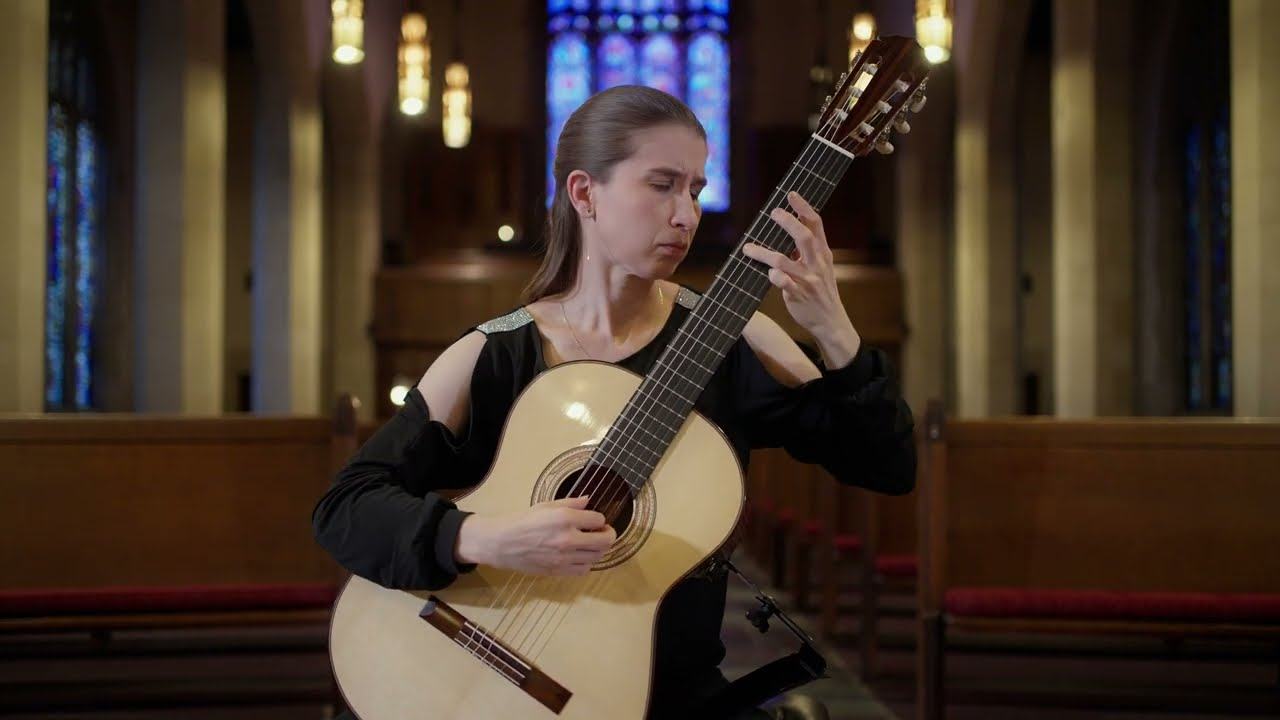
\includegraphics[width=0.48\linewidth]{pictures/youtube/2024/12/20241228_012223_youtube_001_QM66vhlGPfA.jpg}
}
\end{center}




聖母の御子、盗賊の歌に続いて、一連の \#カタロニア民謡 から攻略したい曲の３曲目は、\#アメリアの遺言 です。添付は \#リョベート編 だろうと思います。


この方（添付）の演奏には、以前シャコンヌの演奏でも感心して聞いたけれども、演奏の正確さに起因するものなのか、毅然とした厳しさみたいな雰囲気を感じます（←プロの演奏家は皆さんそういうものなのかな）。また映像の途中、右手に接近して上から撮影されている所があって、\#人工ハーモニクス を演奏する際の指の格好などは参考になります。


短い曲だけど、人工ハーモニクスがいっぱいで、その部分はとても難しいです（私には）。先ずはハーモニクス無しで、左手だけを攻略してしまう必要がありそうです。

\subsection*{2024年12月28日 01:23}
\addcontentsline{toc}{subsection}{2024年12月28日 01:23}

\paragraph{リンク}
\url{https://youtu.be/ReNitcL2PIs}

\begin{center}
\href{https://youtu.be/ReNitcL2PIs}{
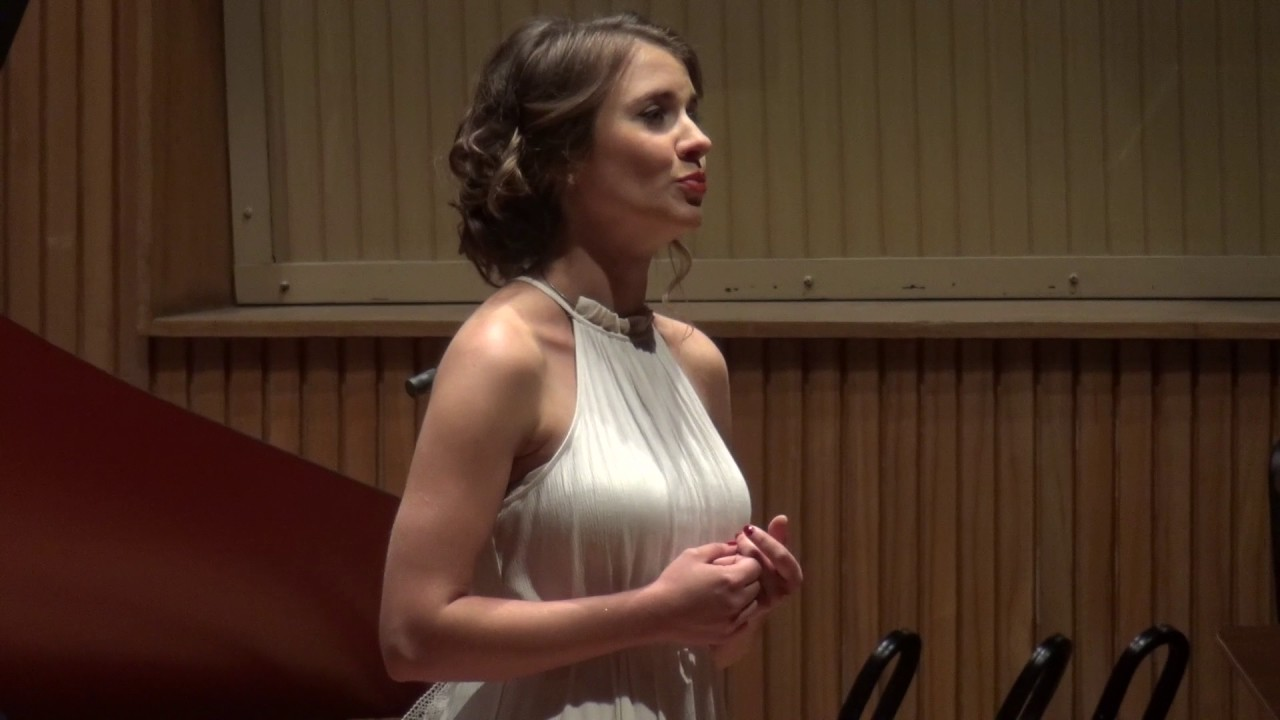
\includegraphics[width=0.48\linewidth]{pictures/youtube/2024/12/20241228_012317_youtube_001_ReNitcL2PIs.jpg}
}
\end{center}

\subsection*{2024年12月28日 01:24}
\addcontentsline{toc}{subsection}{2024年12月28日 01:24}

\paragraph{リンク}
\url{https://youtu.be/dADKgXLcdvo}

\begin{center}
\href{https://youtu.be/dADKgXLcdvo}{
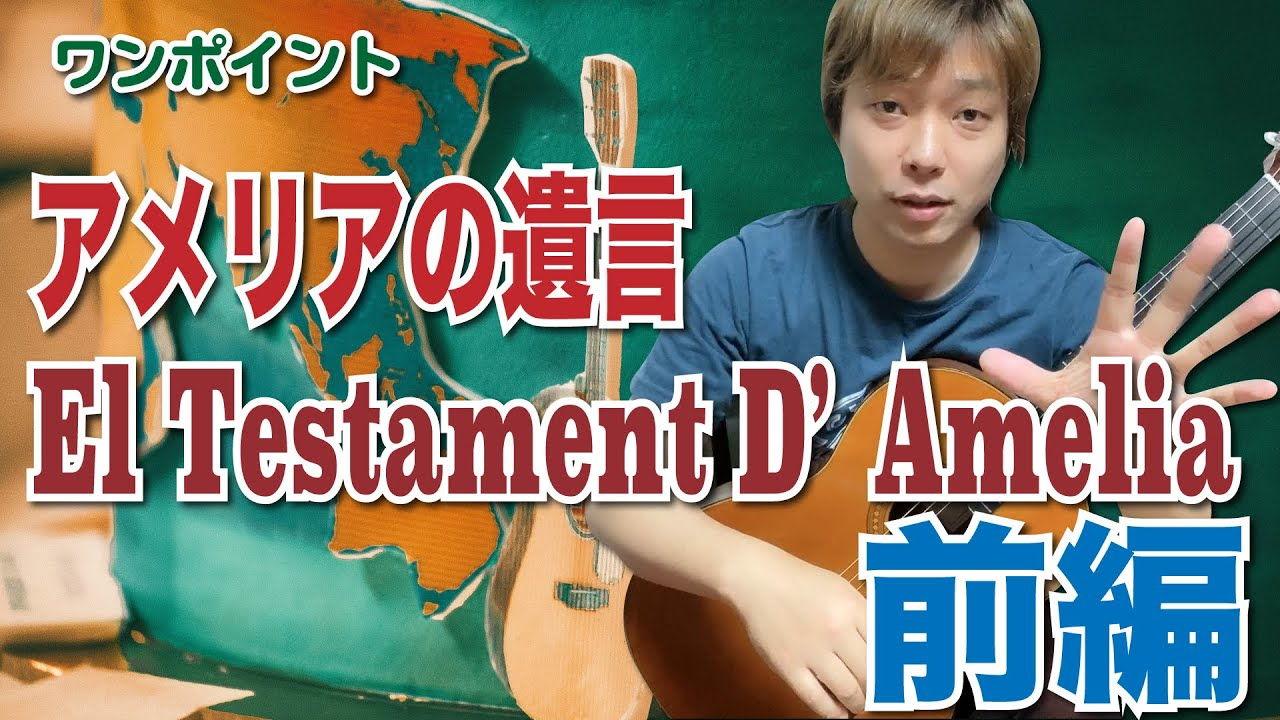
\includegraphics[width=0.48\linewidth]{pictures/youtube/2024/12/20241228_012405_youtube_001_dADKgXLcdvo.jpg}
}
\end{center}

\subsection*{2024年12月28日 10:14}
\addcontentsline{toc}{subsection}{2024年12月28日 10:14}

\paragraph{リンク}
\url{https://www3.nhk.or.jp/news/special/nobelprize/2022/physics/article_12.html}

\subsection*{2024年12月28日 15:09}
\addcontentsline{toc}{subsection}{2024年12月28日 15:09}

\paragraph{リンク}
\url{https://youtu.be/QVVxeHj-ENE}

\begin{center}
\href{https://youtu.be/QVVxeHj-ENE}{
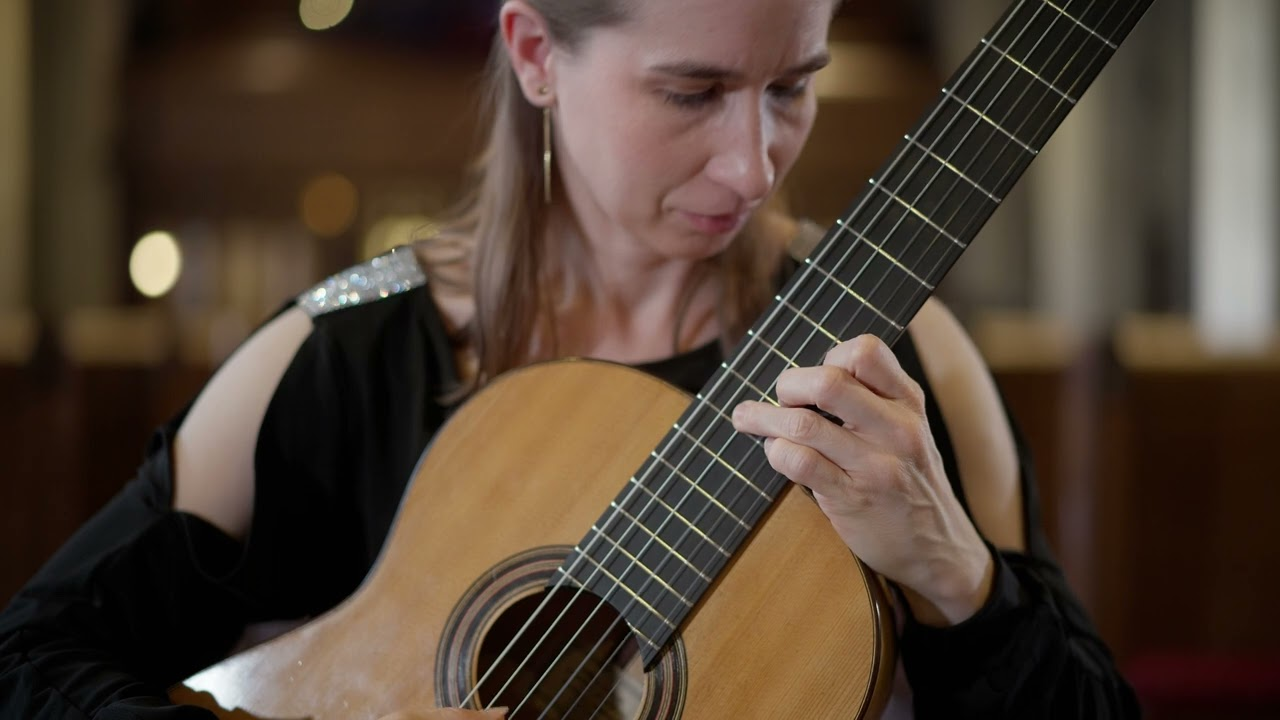
\includegraphics[width=0.48\linewidth]{pictures/youtube/2024/12/20241228_150902_youtube_001_QVVxeHj-ENE.jpg}
}
\end{center}

\subsection*{2024年12月28日 20:00}
\addcontentsline{toc}{subsection}{2024年12月28日 20:00}

\paragraph{リンク}
\url{https://nazology.kusuguru.co.jp/archives/167844}

\subsection*{2024年12月29日 22:59}
\addcontentsline{toc}{subsection}{2024年12月29日 22:59}

\paragraph{リンク}
\url{https://youtu.be/7zabfWdddBc}

\begin{center}
\href{https://youtu.be/7zabfWdddBc}{
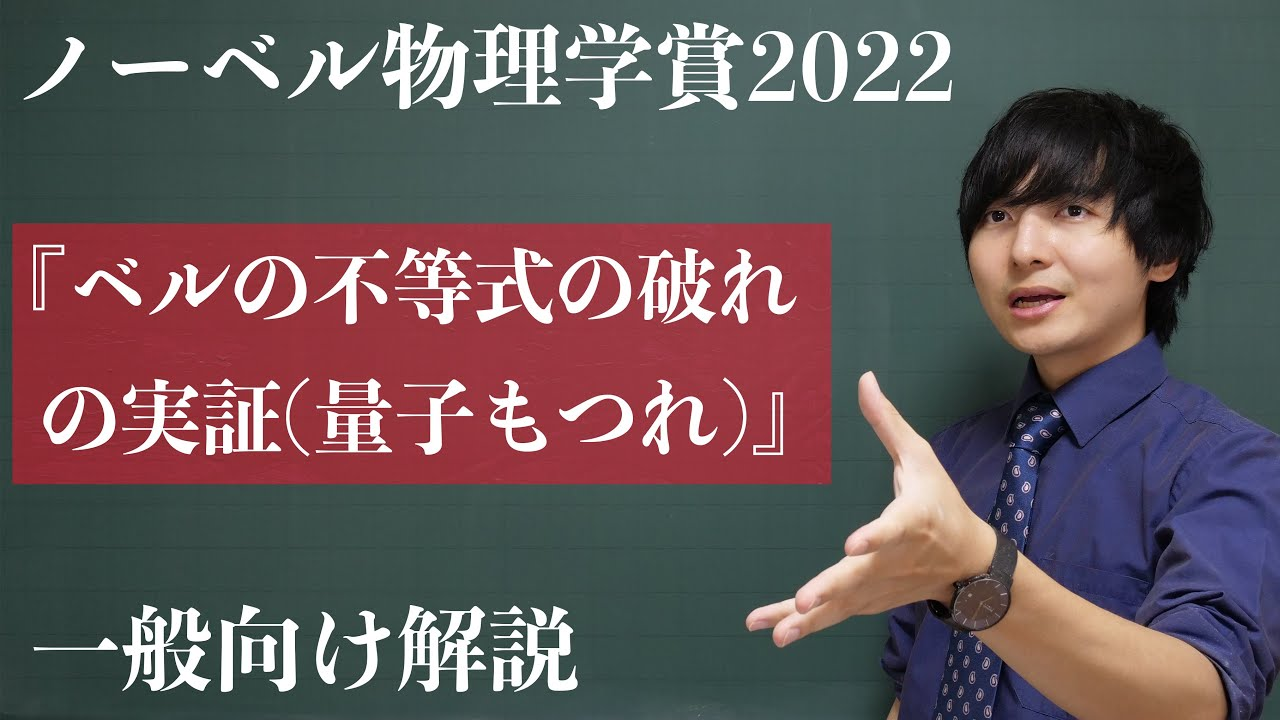
\includegraphics[width=0.48\linewidth]{pictures/youtube/2024/12/20241229_225903_youtube_001_7zabfWdddBc.jpg}
}
\end{center}

\subsection*{2024年12月29日 23:04}
\addcontentsline{toc}{subsection}{2024年12月29日 23:04}

\paragraph{リンク}
\url{https://youtu.be/O99Zy-6YwoU}

\begin{center}
\href{https://youtu.be/O99Zy-6YwoU}{
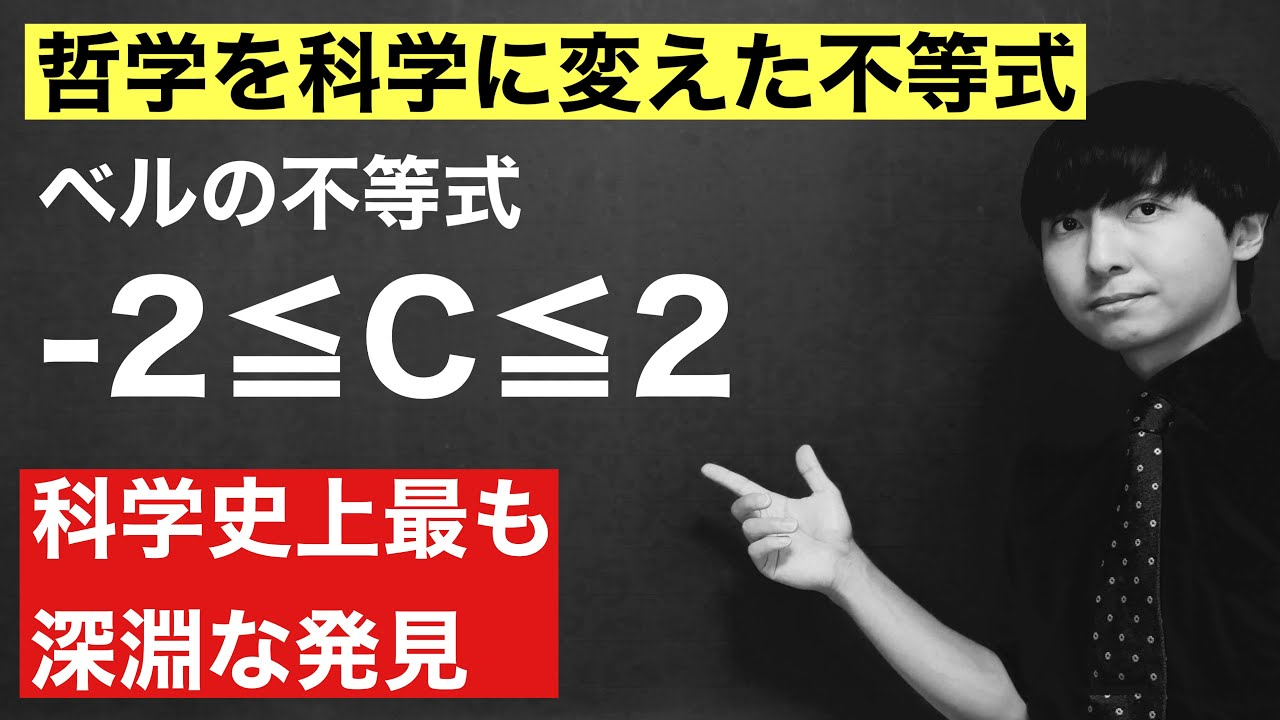
\includegraphics[width=0.48\linewidth]{pictures/youtube/2024/12/20241229_230421_youtube_001_O99Zy-6YwoU.jpg}
}
\end{center}

\subsection*{2024年12月30日 08:56}
\addcontentsline{toc}{subsection}{2024年12月30日 08:56}

\paragraph{リンク}
\url{https://youtu.be/2MOTNxNYwdM}

\begin{center}
\href{https://youtu.be/2MOTNxNYwdM}{
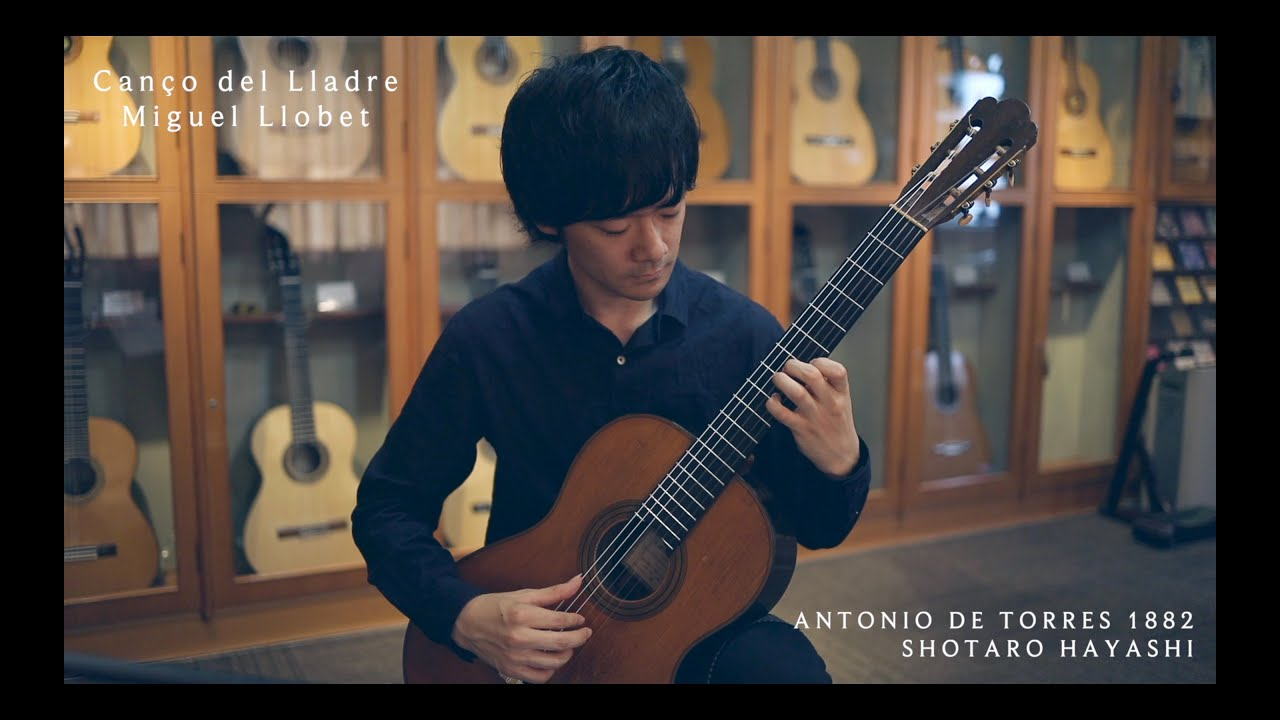
\includegraphics[width=0.48\linewidth]{pictures/youtube/2024/12/20241230_085649_youtube_001_2MOTNxNYwdM.jpg}
}
\end{center}

\subsection*{2024年12月30日 20:06}
\addcontentsline{toc}{subsection}{2024年12月30日 20:06}

\paragraph{リンク}
\url{https://youtu.be/sLY7KTalpis}

\begin{center}
\href{https://youtu.be/sLY7KTalpis}{
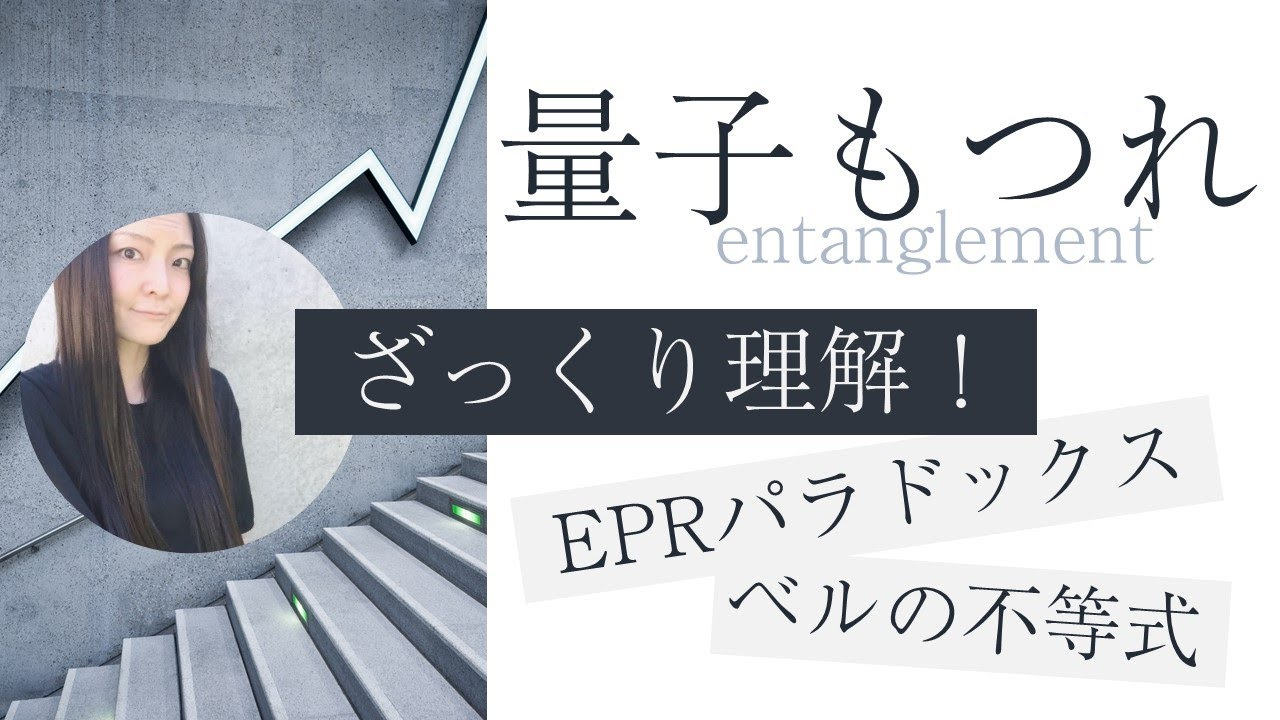
\includegraphics[width=0.48\linewidth]{pictures/youtube/2024/12/20241230_200608_youtube_001_sLY7KTalpis.jpg}
}
\end{center}

\subsection*{2024年12月30日 20:07}
\addcontentsline{toc}{subsection}{2024年12月30日 20:07}

\paragraph{リンク}
\url{https://youtu.be/lD8LYAK0tqs}

\begin{center}
\href{https://youtu.be/lD8LYAK0tqs}{
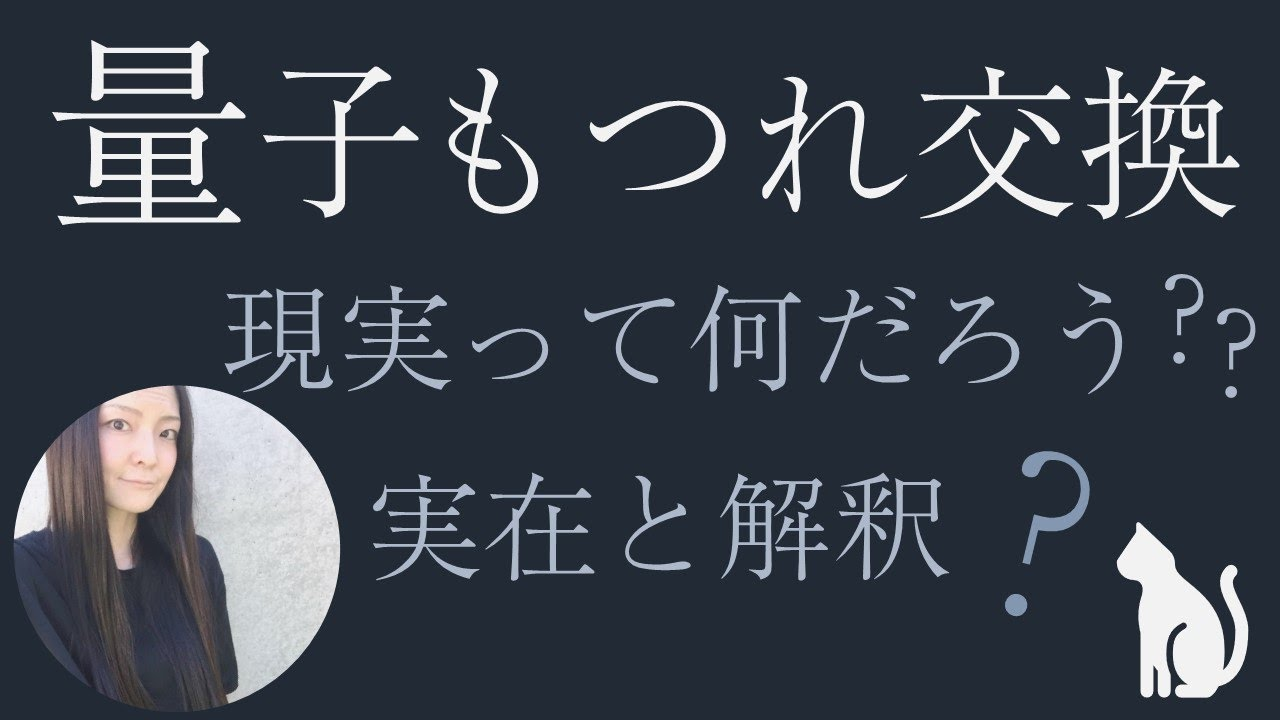
\includegraphics[width=0.48\linewidth]{pictures/youtube/2024/12/20241230_200725_youtube_001_lD8LYAK0tqs.jpg}
}
\end{center}


\end{document}
